%%%%%%%%%%%%%%%%%%%%%%%%%%%%%%%%%%%%%%%%%%%%%%%%%%%%
%%%     Language Science Press Master File       %%%
%%%         follow the instructions below        %%%
%%%%%%%%%%%%%%%%%%%%%%%%%%%%%%%%%%%%%%%%%%%%%%%%%%%%

% Everything following a % is ignored
% Some lines start with %. Remove the % to include them
% You can skip to line 41

\documentclass[output=book,
  colorlinks,citecolor=brown
%  ,draft
% ,draftmode,
%  booklanguage=german,
		  ]{langscibook}
%%%%%%%%%%%%%%%%%%%%%%%%%%%%%%%%%%%%%%%%%%%%%%%%%%%%
%%%          additional packages                 %%%
%%%%%%%%%%%%%%%%%%%%%%%%%%%%%%%%%%%%%%%%%%%%%%%%%%%%
\author{Dominic Schmitz} 
\title{Production, perception, and comprehension of subphonemic detail}
\subtitle{Word-final /s/ in English}
% \ISBNdigital{}
% \ISBNhardcover{}
% \BookDOI{}
% \typesetter{}
% \proofreader{}
% \lsCoverTitleSizes{51.5pt}{17pt}
\renewcommand{\lsSeries}{} 
\newcommand{\lsSeriesTitle}{} 
\newcommand{\lsSeriesColor}{purple} 
\renewcommand{\lsSeriesNumber}{} 

\usepackage{langsci-optional}
\usepackage{langsci-gb4e}
\usepackage{langsci-lgr}

\usepackage{listings}
\lstset{basicstyle=\ttfamily,tabsize=2,breaklines=true}

% my packages
\usepackage{svg} 
\usepackage{qtree}
\usepackage{multicol}
\usepackage{linguex}
\usepackage{tikz-qtree}
\usepackage{tikz-qtree-compat}
\usepackage{multirow}
\usepackage{rotating}
\usepackage{blkarray}
\usepackage{langsci-branding}

\input{localhyphenation.tex}
\addbibresource{localbibliography.bib}
%%%%%%%%%%%%%%%%%%%%%%%%%%%%%%%%%%%%%%%%%%%%%%%%%%%%
%%%             Frontmatter                      %%%
%%%%%%%%%%%%%%%%%%%%%%%%%%%%%%%%%%%%%%%%%%%%%%%%%%%%
\include{localhyphenation}
\begin{document}
\newcommand*{\orcid}{}


\maketitle
\frontmatter
\currentpdfbookmark{Contents}{name} % adds a PDF bookmark
{\sloppy\tableofcontents}
%% remove the % in the following lines if your book has these elements
%  \include{chapters/preface}
\addchap{\lsAcknowledgementTitle} 

Thank you to Ingo Plag and Dinah Baer-Henney. Without your ideas my dissertation, of which this book is a slightly altered version, would not have been possible. Thank you for your invaluable expertise and enthusiasm, for listening to my ideas and questions, and for providing a constant flow of new input. Thank you for guiding me through my PhD and for pushing me to sharpen my thinking.

Thank you to Arne Lohmann, who always had an open door and open ear for my questions.

Thank you to everyone in the DFG research unit Spoken Morphology for listening to talks on word-final /s/ over and over again, and for giving me insightful feedback. 

Thank you to the Deutsche Forschungsgemeinschaft for funding the research unit, giving me the opportunity to fully concentrate on my research.

Thank you to James White and Andrew Nevins for giving me the opportunity to run my production experiment at Chandler House, University College London, and to Andrew Clark for his technical support.

Thank you to Yu-Ying Chuang for providing help, support, and valuable input on my linear discriminative learning implementation. Without your input my LDL study would not have been possible.

Thank you to Jennifer Hay for making it possible to conduct my perception and comprehension experiments at the University of Canterbury, Christchurch, and to Wakayo Mattingley and Gia Hurring who run them on site. Thank you to Jessie Nixon for providing recordings for the experiments. I am very grateful for your help in times of global turmoil.

Thank you to everyone in the English linguistics department at the Heinrich-Heine-Universität Düsseldorf. A great team of colleagues makes working on your PhD much easier. A special thanks to Viktoria, Simon, and Marie who listened to my complaints, and provided feedback and food for thought wherever and whenever necessary.

Thank you to Julika, Sally, Jennifer, Lisa-Marie, Ann-Sophie, Nina, and Lukas for the countless hours you spent in front of Praat, for pilot-testing my perception and comprehension experiments, and for proofreading my work.

Thank you to my best friend, Janina, who provided invaluable mathematical insight and stimulating discussions as well as happy distractions to rest my mind outside my research.

Thank you to my family for having faith in me, for your sympathetic ear, and for reminding me that there is more than word-final /s/ in the world.

Thank you to my partner, Dennis, for your love, patience, and support, and most of all, for always believing in me.



%  \include{chapters/abbreviations}
\mainmatter

%%%%%%%%%%%%%%%%%%%%%%%%%%%%%%%%%%%%%%%%%%%%%%%%%%%%
%%%             Chapters                         %%%
%%%%%%%%%%%%%%%%%%%%%%%%%%%%%%%%%%%%%%%%%%%%%%%%%%%%

%\chapter{Introduction}\label{chapter01}

The complexities of speech production, perception, and comprehension are enormous. This circumstance has led to the development of numerous models and theories of language production, perception, and comprehension since the dawn of the modern study of language structures in the early twentieth century. Especially since the rise of psycholinguistics in the 1960s, psycholinguistic methods and findings contributed to the development of pertinent theoretical approaches to language structure. As has been shown repeatedly in recent linguistic research, however, it remains a challenge for most if not all established approaches to account for findings on more and more intricate features of language such as differences in subphonemic detail.

In research on speech production, it was shown that homophonous lexemes differ in their acoustic duration due to differences in frequency (e.g. \cite{Jurafsky2002, Lavoie2002, Gahl2008, Drager2011, Lohmann2018}). Such findings indicate that phonologically identical lemmas may differ in their phonetic realisation. Similarly, fine phonetic differences were also found, for example, for bound versus free bases (e.g. \cite{Kemps2005a, Kemps2005b}), for final segments of a mono-morphemic stem versus the final segments of the same stem if followed by a suffix (e.g. \cite{Sugahara2004, Sugahara2009}), and for prefixes in prefixed versus so-called pseudo-prefixed words (e.g. \cite{Smith2012}). A popular case for the research of such fine-grained phonetic detail below the word level is word-final /s/ and /z/ in English. Previous corpus studies (\cite{Zimmermann2016, Plag2017, Tomaschek2019}) showed that the acoustic duration of word-final /s/ depends on its morphological make-up, with non-morphemic /s/ being longest and auxiliary clitic /s/ being shortest in duration. However, previous experimental studies (\cite{Walsh1983, Hsieh1999, Seyfarth2017}) found effects in the opposite direction. It is thus the first general aim of this book to investigate by means of a production task whether such durational differences between different types of word-final /s/ really exist, and to find a potential explanation for the contradictory nature of previous results. I will introduce relevant theoretical approaches of speech production such as feed-forward formal theories of morphology-phonology interaction (e.g. \cite{Chomsky1968, Kiparsky1982}), the framework of Prosodic Phonology (e.g. \cite{Booij1983, Nespor2007}), psycholinguistic theories of speech production (e.g. \cite{Levelt1999, Roelofs2019}), exemplar-based models (e.g. \cite{Goldinger1998, Pierrehumbert2001, Gahl2006}), and discriminative learning (e.g. \cite{Rescorla1988, Ramscar2007, Ramscar2010}) to discuss their respective explanatory limits. As the approach of discriminative learning can only be meaningfully discussed in light of an implementation of such an approach, a linear discriminative learning network (e.g. \cite{Baayen2019}) is implemented. This implementation not only allows for a discussion of the general approach itself, but potentially offers insight into the nature of the durational differences in word-final /s/.

Research on the perception of fine phonetic detail found that listeners make use of segment durations as a cue for word boundaries (\cite{Shatzman2006}) and to assist in differentiating phonologically similar lemmas (\cite{Warner2004}). Findings on bare versus suffixed stems indicate that listeners make use of acoustic duration as a cue for distinguishing such stems (\cite{Kemps2005a, Kemps2005b, Blazej2015}). Yet, there is barely any research on the question of how small such subphonemic durational differences may be to remain perceptible. This question is answered for individual segments by a rather dated study by \citet{Klatt1975}. That is, to be perceptible, a durational difference in fricatives should be of 25 ms or more. However, these authors found that perceptibility is worse in fricatives and word-final position. Hence, the second general aim of this book is to explore how small a durational difference in word-final /s/ is perceptible in a same-different perception task. I will discuss the findings taking into account abstractionist approaches (e.g. \cite{Klatt1979, McClelland1986, Norris1994, Norris2008}), approaches relying on fine phonetic detail (e.g. \cite{Goldinger1996}), approaches combining abstract representations and fine phonetic detail (e.g. \cite{Hawkins2001, Pierrehumbert2002}), and computational models of speech perception (e.g. \cite{tenBosch2015, Baayen2019}).

\largerpage
For an account of the influence of subphonemic detail on comprehension, one can consider the same results which have been brought forward to describe the perception of such fine phonetic detail. As subphonemic durational differences are used as a cue for word boundaries (\cite{Shatzman2006}), they are not only perceptible but also used in the comprehension of words. Differentiating between unsuffixed and suffixed stems by means of acoustic durations (\cite{Kemps2005a, Kemps2005b, Blazej2015}) does not only indicate that such differences are perceived, but also that such differences are made use of in comprehension. In general, however, there is little research available which directly asks the question of whether subphonemic durational differences significantly influence comprehension (e.g. \cite{Blazej2015}). Thus, it is the third general aim of this book to investigate this question. This is done by means of two number-decision tasks in a mouse-tracking paradigm. Taking into account the findings from these experiments, I will discuss the same set of theoretical approaches as are taken into account for the results of the perception study: abstractionist approaches, approaches relying on fine phonetic detail, approaches combining abstract representations and fine phonetic detail, and computational models of speech perception. 

\largerpage
The overarching goal of this book, then, is to draw a more detailed, intricate, and exhaustive picture of the production, perception, and comprehension of subphonemic detail. To achieve this goal, two important methodological decisions were taken. First, where applicable, pseudowords as well as real words are used as target items to account for potentially confounding effects of lexical properties (e.g. effects of frequency, e.g. \cite{Gahl2008, Lohmann2018}; effects of storage, e.g. \cite{Caselli2016}). Second, sound statistical analyses are performed, relying on novel statistical techniques where appropriate. Overall, the findings presented in this book are the results of a thorough methodological approach to item design and statistical analysis, offering a reliable account of the nature of subphonemic detail and a strong foundation for future research.

This book is structured as follows. In Chapter \ref{chapter02}, I will give a detailed overview of previous findings on the production, perception, and comprehension of subphonemic durational differences and introduce pertinent theoretical approaches. Taking these approaches as a starting point, hypotheses to be investigated in the subsequent chapters are derived. Chapter \ref{chapter03} will introduce the general method used in this book. It will discuss pseudowords as a type of item (Section \ref{section03_1_1}) and present the pseudoword and real word items used across all studies of this book (Section \ref{section03_1_2}). Statistical methods and procedures are described in Section \ref{section03_2}. Then, the approach of linear discriminative learning is introduced (Section \ref{section03_3}). Chapter \ref{chapter04} presents the production study investigating the production of subphonemic durational differences in word-final /s/, while Chapter \ref{chapter05}, relying on the introduction to linear discriminative learning in Section \ref{section03_3}, presents the implementation of such a linear discriminative learning network to account for the nature of the reported subphonemic durational differences. In Chapter \ref{chapter06}, I will present the perception study, which consists of a same-different task to investigate the perceptibility of durational differences in word-final /s/. Chapters \ref{chapter07} and \ref{chapter08} introduce and discuss the two number-decision tasks used to examine the influence of subphonemic durational differences on comprehension. In Chapter \ref{chapter09}, I will bring together the results of the individual studies presented in Chapters \ref{chapter04} to \ref{chapter08} and discuss them in light of the general aims set in the present and the hypotheses given the following chapter. Chapter \ref{chapter10} concludes this book.

\chapter{Subphonemic differences in phonologically identical elements}\label{chapter02}

Research of the last decades has repeatedly shown that subphonemic differences are found in the production of phonologically identical elements (\cite{Walsh1983, Hsieh1999, Cho2001, Jurafsky2002, Lavoie2002, Sugahara2004, Sugahara2009, Kemps2005a, Kemps2005b, Gahl2008, Drager2011, Smith2012, Zimmermann2016, BenHedia2017, Plag2017, Seyfarth2017, Lohmann2018, BenHedia2019, Tomaschek2019, Plag2020}) and that such differences can be perceived as well as be used in comprehension (e.g. \cite{Klatt1975, Warner2004, Kemps2005a, Kemps2005b, Shatzman2006}). It is on these findings that the research presented in this book is grounded. Instead of following a specific theory that is to be confirmed, the studies this book reports on are of an explorative nature. The research questions addressed in the individual studies are met with all relevant theories at hand to provide elaborate discussions of the respective findings. The exploratory nature of this research is typical of research spanning multiple areas of a discipline. In the present case, findings, concepts, and approaches of morphology, phonology, phonetics, computational linguistics, and psycholinguistics are combined. While this at times may prove difficult, it also enriches the knowledge gain of the field by combining theoretical accounts spanning different subdisciplines. The overall aim of the approach in this book follows its overarching aim of establishing substantiated knowledge on subphonemic detail and its role in production, perception, and comprehension. 

Previous findings as well as the main theoretical accounts concerning the production, perception, and comprehension of subphonemic detail are introduced in the following sections, Section \ref{section02_1} and Section \ref{section02_2}, respectively. In both sections, I will first review relevant previous empirical findings before I then introduce pertinent theoretical approaches and models. Taking the theoretical accounts as motivation, I will derive the hypotheses to be explored in the studies of this book. Finally, I will sum up the hypotheses for a concise overview in Section \ref{section02_3}.

\section{Production}\label{section02_1}

The evidence for the presence of morphological information at the subphonemic level emerges mainly from the study of homophonous lexemes, stems, and affixes.\protect\footnote{An earlier version of this section has been published in \protect\citet{Schmitz2021a}.} For homophonous lexemes, \citet{Gahl2008} and \citet{Lohmann2018} investigated acoustic realisations of seemingly homophonous word pairs such as \textit{time} and \textit{thyme} and found the more frequent member of each pair to be of shorter acoustic duration. Further evidence for differing acoustic realisations of supposedly homophonous lexemes was found by \citet{Drager2011}. Drager compared realisations of \textit{like} as adverb, verb, discourse particle, and as part of the quotative \textit{be like}. Differences surfaced in several phonetic parameters. Similar effects were found for function words such as \textit{four} and \textit{for} and different uses of words such as \textit{to}, which were investigated by \citet{Lavoie2002} and \citet{Jurafsky2002}. Such fine realisational differences indicate that at the phonetic level, two or more phonologically homophonous lemmas may differ in their realisation.

Similarly, evidence shows that seemingly homophonous elements below the word level have different phonetic realisations. \citet{Kemps2005a} and \citet{Kemps2005b} found that in Dutch and English segmentally identical free and bound variants of a base (e.g. \textit{help} without a suffix versus \textit{help} in \textit{helper}) differ acoustically. \citet{Sugahara2004,Sugahara2009} found phonetic differences between the final segments of a mono-morphemic stem as compared to the final segments of the same stem if followed by a suffix, e.g. in \textit{mist rain} versus \textit{missed rain}. The stem had slightly longer rhymes if followed by certain suffixes. \citet{Seyfarth2017} found that for words ending in fricatives, the durations of a word’s morphological relatives influence the realisation of that word. In their study, stems of multi-morphemic words showed longer durations than similar strings of segments in homophonous mono-morphemic words (e.g. \textit{free} in \textit{frees} versus \textit{freeze}). They concluded that the durational targets of the multi-morphemic word’s relatives influence the word’s duration to such an extent that a durational difference between the respective multi-morphemic word and its homophonous mono-morphemic counterpart arise. A similar effect of morphological relations influencing duration was found for plurals and their bare stems in a corpus-based study by \citet{Engemann2021}.

For prefixes, \citet{Smith2012} found systematic realisational differences for \textit{dis}- and \textit{mis}- between prefixed and so-called pseudo-prefixed words (e.g. \textit{discolour} versus \textit{discover}). Prefixed words showed longer durations and longer voice onset times, among other things. \citet{BenHedia2017} and \citet{BenHedia2019} showed that the more segmentable a prefix, the longer the duration of its nasal.

On the articulatory level, \citet{Cho2001} found evidence for the variability of intergestural timing between identical strings in mono- versus multi-morphemic contexts. In their electropalatographic study, Cho showed that the timing of the gestures for [ti] and [ni] in Korean show more variation when the sequence is mono-morphemic (/mati/ ‘knot’ and /pani/ ‘name’) as compared to the timing of the same gestures in multi-morphemic sequences (/mat-i/ ‘the oldest’ and /pan-i/ ‘class-\textsc{nom}’), thus indicating that morphological structure is reflected in articulatory gestures, which in turn may lead to correlates in the acoustic signal. Hence, morphology is reflected in the phonetic realisation of otherwise identical strings of segments.

In sum, it seems that there is vast evidence for seemingly homophonous elements, that is, lexemes, bases, and affixes, to differ on the level of speech production. Differences on the level of segments have been reported as well. Previous corpus studies on word-final /s/ in English found realisational differences between non-morphemic, suffix, and clitic variants. \citet{Zimmermann2016} on New Zealand English (data from QuakeBox corpus; \cite{Walsh2013}) and \citet{Plag2017} as well as \citet{Tomaschek2019} on North American English (data from Buckeye Corpus of Conversational Speech; \cite{Pitt2007}) found that non-morphemic /s/ showed longer durations than suffix and clitic /s/. In turn, suffix /s/ also showed longer durations than clitic /s/. While these results draw a clear picture of /s/ duration across morphological categories (including the non-morphemic /s/), they are subject to unbalanced data sets due to the nature of corpora. That is, corpus data may contain a huge number of confounding and moderator variables that experimental data can control for (e.g. \cite{Gries2015}).

Previous experimental studies, however, have reported less consistent results and show some problematic methods and analyses. \citet{Walsh1983} carried out a production experiment with three homophonous word pairs (e.g. \textit{Rex} and \textit{wrecks}). They measured the duration of the word-final /s/ in both the mono- and the multi-morphemic word of each pair in three different conditions. Each word was produced by eight to ten participants. Condition I consisted of an unambiguous context; condition II consisted of a semantically neutral context; condition III consisted of a semantically anomalous context.  While in two of these conditions there was a small difference of 9 ms in the means of the different types of /s/, there was none in the third condition. Still, the authors concluded that ``speakers of English systematically lengthen morphemic /s/" (\cite[204]{Walsh1983}). However, their analysed data set was small (110 observations), included a mixture of common and proper nouns, and no phonetic covariates were integrated in their analysis. Further, instead of applying appropriate inferential statistical methods (e.g. t-tests or more advanced methods), the mean durations of the types of /s/ under investigation were compared impressionistically. Therefore, there are several reasons to be sceptical of their results.

In another study, \citet{Hsieh1999} measured /s/ duration in child-directed speech in data originally elicited for another study (on vowel durations in function words, see \cite{Swanson1994}). The authors found plural /s/ to be longer than third-person singular /s/. However, as the data originally was not designed for this endeavour, half of all plural items occurred sentence-finally, while almost all third-person singular items occurred sentence-medially. The durational difference found between the suffixes may hence have been due to effects of phrase-final lengthening (e.g. \cite{Klatt1976,Wightman1992}) rather than to inherent phonetic differences due to morphological categories. 

In a more recent study, \citet{Seyfarth2017} conducted a production experiment to collect data on non-morphemic, plural, and third-person singular /s/ and /z/ durations. They found the non-morphemic variant to be shorter than the morphemic instances. However, they did not find differences between the voiced and the voiceless allomorphs during their analysis. This may be a worrisome result, especially considering the small number of items with voiceless allomorphs (n = 6) as compared to the high number of items with voiced allomorphs (n = 20) in their data. 

Recently, \citet{Plag2020} found plural and genitive plural /s/ to be of different durations. In their study, the genitive plural suffix showed significantly longer durations as compared to the plural suffix. An overview of the durational differences found in the aforementioned experimental studies is given in \ref{tab:2.1}.

\begin{table}\fontsize{10}{11}
\caption{Overview of durational differences of word-final /s/ found in previous studies.}
\label{tab:2.1}
\begin{tabular}{ll}
\lsptoprule
Study                                & Findings                                         \\
\midrule
\cite{Zimmermann2016, Plag2017}, & \multirow{2}{*}{non-morphemic $>$
plural $>$ clitics}  \\
\cite{Tomaschek2019}               &                                                  \\
\cite{Walsh1983}                  & plural $>$ non-morphemic                            \\
\cite{Hsieh1999}                   & plural $>$ third-person singular                    \\
\cite{Seyfarth2017}                & plural $>$ non-morphemic                            \\
\cite{Plag2020}                    & genitive plural $>$ plural                 \\
\lspbottomrule
\end{tabular}
\end{table}

In sum, there is evidence that there may be durational differences between different types of /s/. However, while results of corpus studies are in line with each other, they might be flawed due to imbalanced data sets. Previous experimental studies, on the other hand, have often relied on small data sets and lacked phonetic covariates, appropriate statistical methods, or a proper distinction of voiced and voiceless segments. Another crucial difference between corpus and experimental studies is the use of homophones. While all previous experimental studies restricted their data to homophone pairs, corpus studies take into consideration all words. The limitation to homophones and the resulting competition between their representations might be a problem in itself, as it appears to be unclear how members of homophone pairs are stored and connected to their respective frequencies. In all cases, previous results were subject to potentially confounding effects of the lexical properties (e.g. effects of frequency, e.g. \cite{Gahl2008,Lohmann2018}; effects of storage, e.g. \cite{Caselli2016}) and contextual effects (e.g. phrase final lengthening, e.g. \cite{Klatt1976,Wightman1992}) of the items under investigation. Also, so far, no experimental study included clitics in their analysis, whereas corpus studies have suggested that clitics show different durations than suffixes.

A study is therefore called for that investigates the durational nature of different types of word-final /s/ in English, preferably an experimental study with carefully controlled data avoiding potentially confounding effects. This book presents such a study investigating word-final /s/ in English by means of a pseudoword production task. In this task, three types of word-final /s/ were elicited: mono-morphemic, plural, and clitic /s/ (with the auxiliaries \textit{is} and \textit{has}). It will address some of the issues of previous studies. More precisely, the use of pseudowords prevents potential lexical effects to confound findings (see Section \ref{section03_1_1}), while the highly controlled task evades the influence of contextual effects. Even though the data will also contain homophone pairs to a certain extent, the individual members do not have lexical representations. That is, one can rule out effects of competition between homophonous lexical entries due to their similar representations. In addition, the use of pseudowords eliminates potential differences in duration due to differences in frequency between the homophones.

Let us now turn to the question of how morpho-phonetic effects can be explained at the theoretical level. Existing theories make different predictions concerning the possible presence of durational differences between different types of /s/. I will discuss four approaches here: feed-forward models of phonology-morphology interaction, Prosodic Phonology, exemplar theory, and discriminative learning. 

In standard feed-forward formal theories of morphology-phonology interaction, all types of /s/, be they morphemic or non-morphemic, are treated in a similar way (e.g. \cite{Chomsky1968,Kiparsky1982}). In the case of morphological word-final /s/, a process called \textit{bracket erasure} is said to remove all morphological information from a pertinent word form once retrieved from the lexicon during the stage of \textit{lexical phonology} and leaves speech production without an insight into the morphological makeup at the stage of \textit{post-lexical phonology}. After retrieval, there is no informational difference between word-final morphemic and non-morphemic types of /s/. Thus, there is nothing in such a system that could account for realisational differences, e.g. different durations, between phonologically identical suffixes and non-morphemic segments. The realisation of clitics is a post-lexical process to begin with and thus outside the scope of any prediction by this theory.

In the framework of Prosodic Phonology, there is a complex mapping of morphological structure onto prosodic structure (\cite{Booij1983,Nespor2007}). Since prosodic boundaries may correlate with particular phonetic properties, segments at such boundaries may show systematic differences in phonetic implementation (see, for example, \cite{Keating2006}). Phonetic differences between two phonologically homophonous affixes could therefore result from a difference in the prosodic structure that goes with the two affixes. In particular, different types of word-final /s/ can be analysed as having different positions in the hierarchical prosodic configuration. These configurations co-determine the degree of integration of an /s/ to the word it belongs to. These different degrees of integration might then emerge as durational differences between types of /s/ in speech production. 

Applying the approach of \citet{Selkirk1996}, non-morphemic /s/, uncontroversially, is an integral part of the prosodic word, as shown in Panel A of Figure \ref{fig:2.1}. \citet{Goad1998} analyses plural /s/ as an \textit{internal clitic}, which is adjoined to the highest prosodic constituent below the prosodic word, as shown in Panel B. In \citet{Goad2002}, however, plural /s/ is analysed as an \textit{affixal clitic}, like third-person singular /s/ in \citet{Goad2003} and \citet{Goad2019}, as shown in Panel C. The prosodic status of the cliticized auxiliary /s/ is not entirely clear, but presumably, it is best analysed as \textit{free clitic}, as in Panel D.

\begin{figure}
    \caption{Prosodic structure of non-morphemic (A), plural (B, C), and clitic /s/ (D) as given in literature on Prosodic Phonology.}
    \label{fig:2.1}
    \centering
\begin{tabular}{llll}
A               & B                 & C                & D              \\
non-morphemic /s/ & plural /s/          & plural /s/         & clitic /s/       \\
                & internal clitic & affixal clitic & free clitic  \\
                ~ & ~ & ~ & ~ \\
\Tree[.PhPhrase [.Pword [.Syllable \textit{bus} ]]]                & 
\Tree[.PhPhrase [.Pword [.Syllable \textit{cat} ] [.\textit{s} ]]]                &
\Tree[.PhPhrase [.Pword [.Pword [.Syllable \textit{cat} ]] [.\textit{s} ]]]  &                
\Tree[.PhPhrase [.Pword [.Syllable \textit{cat} ] ] [.\textit{s} ] ]
\end{tabular}
\end{figure}

The Prosodic Phonology approach thus posits a structural prosodic difference between non-morphemic /s/, plural /s/, and clitic /s/. This prosodic difference might be mirrored in durational differences. It is, however, not so clear what particular phonetic effects this approach would predict and by which processing mechanism the structural prosodic differences would be translated into different articulations. The most plausible prediction would be that closer integration into the prosodic word would correlate with shorter durations: Non-morphemic /s/ should be shortest, clitic /s/ longest, and plural /s/ in between. From the perspective of phrase-final lengthening (e.g. \cite{Klatt1976, Wightman1992}), one should also expect that clitic /s/ is longest, as it immediately precedes a phrase boundary.

The distinction of lexical and post-lexical processing as introduced by the aforementioned standard feed-forward theories of morphology-phonology interaction is also an integral part of established theories in psycholinguistics. According to models of speech production such as the one proposed by Levelt et al. (\cite{Levelt1999}; see \cite{Roelofs2019} for an update), morphemic /s/ would not differ in its realisation from corresponding non-morphemic realisations of /s/. In such models, meanings are stored in the mental lexicon with their forms being represented phonologically. A module called \textit{articulator} uses these phonological forms for speech production, hence, has no information on the lexical origin of particular segments. As a consequence, in this architecture, no systematic differences between different types of /s/ should emerge.

In contrast, exemplar-based models (e.g. \cite{Goldinger1998, Bybee2001, Pierrehumbert2001, Pierrehumbert2002, Gahl2006}) have an architecture that would in principle allow for morpho-phonetic effects. In such models, lexemes are linked to a frequency distribution over their phonetic outcomes as experienced by the individual speaker. These distributions are updated with each new experience: Experienced subtle subphonemic differences then may result in representations mirroring these properties. While such an account may allow for durational differences between different types of word-final /s/ to emerge from stored phonetic representations, it leaves open the question of how such systematic differences between clouds of exemplars would come about in the first place. The downside of this is that it is also unclear in which direction differences between different types of /s/ should play out.

Finally, there is the discriminative learning approach, which is based on simple but powerful principles of discriminative learning theory (\cite{Rescorla1988, Ramscar2007, Ramscar2010}; see, for example, \cite{Baayen2011, Baayen2019} for its application to linguistic problems). According to this theory, learning results from exposure to informative relations among events in the individual’s environment. Individuals use the associations between these events to create cognitive representations of their environment. Most importantly, associations and their resulting representations are updated constantly on the basis of new experiences. Associations are built between features (\textit{cues}, e.g. biphones) and classes or categories (\textit{outcomes}, e.g. different types of /s/) that co-occur in events in which the learner is predicting the outcomes from the cues (\cite{Tomaschek2019}). The relation between cues and outcomes is modelled mathematically by the so-called Rescorla-Wagner equations (\cite{Rescorla1972, Wagner1972, Rescorla1988}). Following these equations, an association strength or \textit{weight} increases every time a cue and an outcome co-occur, while it decreases if a cue occurs without the outcome in a learning event. This results in a continuous recalibration of association strengths, which is a crucial part of discriminative learning. 

In recent discriminative learning implementations, the association weights between semantic representations and phonetic representations have been shown to be predictive of phonetic durations (e.g. \cite{Stein2021}). With regard to final /s/, \citet{Tomaschek2019} show that the different durations of final /s/ can be understood as following from the extent to which words’ phonological and collocational properties can discriminate between the inflectional functions expressed by the /s/. The input features (cues) for their discriminative network were the words (\textit{lexomes} as pointers to the meaning of the forms) in a five-word window centred on the /s/-bearing word and the biphones in the phonological forms of these words. These cues are associated with the inflectional functions of the /s/. Two main measurements emerged as significant predictors of /s/ duration. The so-called \textit{activation} (named \textit{prior} in \cite{Tomaschek2019}) is a measure of an outcome’s baseline activation, i.e. of how well an outcome is entrenched in the lexicon. The other measure is \textit{activation diversity}, which quantifies the extent to which the cues in the given context also support other targets. The general pattern now is the following: When the uncertainty about the targeted outcome increases, the acoustic duration of /s/ decreases. In other words, stronger support (both from long-term entrenchment and short-term from the context) for a morphological function leads to a longer, i.e. enhanced, acoustic signal. 
In sum, the discriminative approach predicts that differences between different types of /s/ may emerge from the associations of form and meaning that speakers develop as a result of their experience with the pertinent words. But what about pseudowords?  It has recently been shown by \citet{Chuang2021} that these associations also play a role for pseudowords. Pseudowords have no representation in the lexicon, but, as these authors show, pseudowords nevertheless resonate with the lexicon due to their formal similarity with existing words. This resonance even influences subtle phonetic details such as duration. It is, however, yet unclear what kinds of durational differences can be expected between different types of /s/ in pseudowords.

Effects of informativity or predictability (which are also inherently present in discriminative learning approaches) are also to mention, as they may play a role as well (\cite{Seyfarth2014, Priva2015, Zee2021}). Greater predictability of the word in its context has been found to lead to phonetic reduction, for example, to shortening in duration. On the other hand, higher paradigmatic predictability has been shown to correlate with longer duration (\textit{paradigmatic enhancement}, e.g. \cite{Kuperman2007, Bell2021}). As these informativity effects are necessarily bound to existing words, an experiment that uses pseudowords cannot straightforwardly test these approaches. 

Based on the different theories laid out above, different hypotheses about durational differences between different types of /s/ in pseudowords can be set up. \textsc{H prod\textsubscript{1}}, the \textit{Feed-Forward Hypothesis}, arises from feed-forward approaches and is in accordance with the prediction that no systematic phonetic differences should be observed between different types of /s/. \textsc{H prod\textsubscript{2}}, the \textit{Prosodic Hypothesis}, is derived from prosodic approaches. According to these approaches, a higher degree of prosodic integration should correlate with shorter durations. Hence, non-morphemic /s/ should be shorter than plural /s/, and plural /s/ should be shorter than clitic /s/. Finally, exemplar-based approaches and discriminative learning approaches both predict the presence of morpho-phonetic effects, but it is unclear how these differences would play out for the three types of /s/ in the present production study. This is encapsulated in \textsc{H prod\textsubscript{3}}, the \textit{Emergence Hypothesis}. 

In summary, the production study presented in Chapter \ref{chapter04} of this book intends to establish whether there are durational differences also with pseudowords, and if so, how these differences play out.

\begin{description}
\item\textsc{H prod\textsubscript{1}}: \textit{Feed-Forward Hypothesis} \newline
There is no durational difference between word-final non-morphemic /s/, plural /s/, and auxiliary clitic /s/.

\item\textsc{H prod\textsubscript{2}}: \textit{Prosodic Hypothesis} \newline
There are durational differences between different types of word-final /s/: 
non-morphemic /s/ is shorter than plural /s/, plural /s/ is shorter than auxiliary clitic /s/.

\item\textsc{H prod\textsubscript{3}}: \textit{Emergence Hypothesis} \newline
There are durational differences between different types of word-final /s/ (non-morphemic, plural, and auxiliary clitic).
\end{description}

\section{Perception and comprehension}\label{section02_2}

Findings on subphonemic durational differences give rise to two further questions. First, are listeners able to perceive such subphonemic durational differences between different types of word-final /s/? That is, are listeners not only sensitive to differences between different phonemes (e.g. \cite{Goldstone2010}) but can they pick up on differences between phonologically similar but phonetically different realisations? Second, if subphonemic durational differences are perceptible, are they used in comprehension? That is, does the perception of (un-)expected subphonemic features influence the comprehension process?

On the level of word perception and comprehension, \citet{Shatzman2006} showed that listeners make use of segment durations as a cue for word boundaries. In their study, native speakers of Dutch listened to ambiguous sentences in which plosive-initial words, e.g. \textit{pot} ‘jar’, were preceded by \textit{eens} ‘once’. Additionally, the sentences could also refer to cluster-initial words instead, e.g. \textit{een spot} ‘a spotlight’. The two readings were, among other acoustic features, different in regard to their /s/ durations: Word-initial /s/ was overall longer in duration than word-final /s/ (Δ = 51 ms). The authors found that listeners make use of such different durations for their lexical decision. That is, the durational difference between word-initial and word-final /s/ was perceptible and used for an informed lexical decision, i.e. in word comprehension.

\citet{Warner2004} investigated whether listeners perceive subphonemic differences in Dutch words of identical phonetic but different underlying phonological form, e.g. /met/ ‘measures (sg.)’ and /med/ ‘avoided (sg.)’, where both words phonetically are transcribed as [meit]. Productions of such word pairs showed differences in the subphonemic features between the members of a pair. One of these features was vowel duration, which listeners showed sensitivity to: Listeners were able to perceive subphonemic detail and to use this information in comprehension, even though differences were rather small, e.g. Δ = 3.5 ms for vowel duration. 

\citet{Kemps2005a} and \citet{Kemps2005b} found that listeners in Dutch and English are sensitive to the durational differences between stems in isolation and stems as parts of affixed word forms, e.g. \textit{help} without a suffix versus \textit{help} in \textit{helper}. This finding is confirmed by similar results in \citet{Lee2020} and in \citet{Blazej2015}. In their study,  Blazej and Cohen-Goldberg showed that listeners make use of duration as a cue for distinguishing unsuffixed stems from suffixed stems, e.g. \textit{clue} without a suffix versus \textit{clue} in \textit{clueless}. The authors found the influence of duration as a cue to be persistent in isolated and continuous speech, with full, reduced, and removed effects of articulation, and in implicit and explicit tasks. 

Taking into account the aforementioned findings, the question arises what the just-noticeable difference to be perceived is. \citet{Klatt1975} found this difference for a change in duration to a single segment to be 25 ms. That is, below the durational difference of 51 ms found in \citet{Shatzman2006} but well above the durational difference of 3.5 ms given in \citet{Warner2004}. Further, according to Klatt and Cooper’s findings, this just-noticeable difference threshold is influenced by several factors. Most importantly, differences in word-final position and differences in fricatives are less well perceptible. 

In sum, evidence for the perception of subphonemic differences in phonologically similar segments and its effect on comprehension exists. However, such evidence is rather sparse and mainly concerned with lexical decisions or differentiation of unsuffixed and suffixed forms. To date, there is no study which looks into the perception and comprehension of phonologically identical but phonetically and morphologically different segments. Thus, two types of studies are called for. First, a study is needed that investigates whether durational differences found between such segments are perceptible. This is the aim of the same-different task I present in Chapter \ref{chapter06} of this book. Using real words as well as pseudowords, potential lexical effects are taken into account. Second, it needs to be investigated whether subphonemic detail is not only perceptible but also used in comprehension. This is the purpose of the two number-decision mouse-tracking tasks I present in Chapters \ref{chapter07} and \ref{chapter08}. Using isolated real words with non-morphemic and plural /s/ in one of the tasks, and pseudowords with plural and clitic /s/ embedded in real word contexts in the other, a detailed image of whether comprehension is affected by subphonemic durational differences is drawn. That is, evidence for real words as well as for pseudowords and for several types of word-final /s/ will be illustrated.

Let us now turn to the question of how the perception and comprehension of subphonemic detail can be explained at the theoretical level. Existing theories of speech perception and comprehension make different predictions concerning the perception of subphonemic detail and its use in comprehension. I will discuss several groups of approaches here: Theories that make use of abstract representations, theories that rely on sets of features, theories that combine abstract representations and sets of features, and computational models of speech perception and comprehension.

In abstractionist models of speech perception, the phonetics of the incoming speech signal are translated into phonemic representations before the stage of lexical access. That is, the result of perception is of phonological nature and without information on phonetic detail. Well known examples of abstractionist approaches are the TRACE model (e.g. \cite{McClelland1986}), Shortlist (e.g. \cite{Norris1994}) and Shortlist B (\cite{Norris2008}) as well as the speech perception and lexical access model introduced by \citet{Klatt1979}. All of these models have in common that perception of subphonemic detail is either considered to be a peripheral process at the margins of speech perception or that it is not considered at all. Additionally, some abstractionist models (e.g. \cite{Klatt1979}) perform time normalisation. Timing (and with that duration) is only conceived as important if it serves a discriminative role, e.g. in stress placement. As this group of abstractionist models does not integrate subphonemic detail in the process of perception, it cannot account for the perception of subphonemic detail and, consequently, its use in comprehension. If subphonemic detail is not considered for the outcome of the perception process, there is no need to perceive it in the first place. Thus, comprehension has no access to any subphonemic, pre-phonological-representation information.

Approaches that make use of features instead of abstract phonemic representations form another group of speech perception models. One such model is the Fuzzy Logical Model of Speech Perception (\cite{Massaro1987}). It assumes that multiple sources of information influence speech perception, that listeners have continuous information about each source, and that the multiple sources are used together in the most meaningful manner. Sources contribute features of sounds as information, which are then used to build so-called summary descriptions. These, in turn, are the result of the perception process. That is, comprehension does not make use of abstract phonological representations as in abstractionist models but of sets of distinct features. Another model based on features was introduced by \citet{Lahiri1991}. Their approach assumes that there is a single underlying phonological representation per lexical item, which is compatible with all phonologically permissible variants of it in a given context. Entailed in such representations is only marked information, i.e. phonetic features. Concerning the perception of subphonemic durational differences, then, one may regard the two aforementioned models as inconclusive. If subphonemic segmental durational differences are accounted for as a meaningful feature, i.e. if it is assumed to be marked information, perception of durational differences in word-final /s/ can be accounted for. Then, such differences can be used in comprehension. If, however, duration is only considered a feature where it distinguishes between phonemes, then perception of subphonemic durational differences is uncalled for. As a consequence, subphonemic durational differences cannot be used in comprehension.

Exemplar-based models of speech perception (e.g. \cite{Goldinger1996}) also rely on features. They assume that individuals draw on a multitude of exemplars per word form, which are all stored in their mental lexicon. Exemplars contain detailed phonetic information, which gives space to information on subphonemic detail. In this regard, exemplar based models account for the perceptibility of subphonemic durational differences, as such differences are stored in exemplars and made use of in perception and comprehension. 

However, previous research has shown that effects attributed to exemplars are not consistently found (e.g. \cite{Hanique2013Aalders}). Such findings are the motivation for hybrid models. One such hybrid model introduced by \citet{Pierrehumbert2002} assumes abstract generalisations as well as exemplars associated with phonological units, that is phonemes, phoneme sequences, and words. While speech production makes use of both abstract representations and exemplars, comprehension mainly relies on the exemplars. Another hybrid model, Polysp (Polysystemic Speech Perception), has been introduced by \citet{Hawkins2001}. Their model assumes that the analysis of acoustic input does not necessarily rely on its transformation into its linguistic units. Rather, it is situation-dependent whether the abstract phonological form of a word or one of its phonetic variants is accessed for comprehension. As phonetic detail is stored in hybrid models, such models can account for the perception of subphonemic differences and the usage of such differences in comprehension.

The final group of approaches to speech perception and comprehension consists of computational models. One such approach is DIANA, an end-to-end computational model of human word comprehension (\cite{tenBosch2015, tenBosch2021}). The implementation of DIANA supports not only the use of abstract units but also takes exemplars, i.e. phonetically rich information, as input for the modelling of comprehension. Thus, it avoids the assumption of a segmental prelexical layer between acoustic signal and the lexical layer, i.e. perception and comprehension. Similarly, linear discriminative learning (\cite{Baayen2019}; see also Sections \ref{section02_1} and \ref{section03_3}) does not assume a segmental representation layer for acoustic input. Instead, it makes use of Frequency Band Summary Features (FBSFs; \cite{Arnold2017}) as representations. FBSFs consist of detailed information of small time intervals of the signal, containing, for example, information on minimum, maximum, median, initial, and final intensity values. The FBSFs of the complete set of acoustic input then are the result of perception, which is a detailed representation of the perceived phonetic signal. This representation is used in comprehension modelling. In sum, both computational approaches, DIANA and linear discriminative learning, assume detailed phonetic information to be the result of perception, and this information is then used for comprehension. Thus, such models can account for the perception of subphonemic differences and their usage in comprehension. 

Based on the approaches laid out above, two hypotheses about the perception of subphonemic durational differences were formulated. \textsc{H perc\textsubscript{1}}, the \textit{Abstractionist Hypothesis}, arises from models of speech perception that have an abstract phonological representation as output of perception. If all fine-grained phonetic detail is lost in perception, one needs not perceive it to begin with. \textsc{H perc\textsubscript{2}}, the \textit{Phonetic Detail Hypothesis}, takes exemplar and hybrid models as well as the aforementioned computational models as a starting point to account for the perception of subphonemic detail. Based on the assumption of storage and usage of detailed phonetic information, subphonemic durational differences can be stored and should thus be perceptible. A hypothesis based on models which make use of features alone is not considered in this book, as predictions on the perceptibility of subphonemic durational differences by such approaches are inconclusive and thus not testable in the current setup.

\begin{description}
\item\textsc{H perc\textsubscript{1}}: \textit{Abstractionist Hypothesis} \newline
Listeners are not sensitive to subphonemic durational differences between different types of word-final /s/.

\item\textsc{H perc\textsubscript{2}}: \textit{Phonetic Detail Hypothesis} \newline
Listeners are sensitive to subphonemic durational differences between different types of word-final /s/.
\end{description}

Finally, \textsc{H comp}, the \textit{Mismatch Hypothesis}, emerges as a consequence of the prior two hypotheses. That is, if fine-grained phonetic detail is perceptible, listeners may make use of it in comprehension. Thus, comprehension should be affected if subphonemic detail does not match its intended meaning or context. This influence may be visible in behavioural data, such as reaction times and mouse trajectories. This hypothesis is supported by the exemplar-based, hybrid, and computational approaches.

\begin{description}

\item\textsc{H comp}: \textit{Mismatch Hypothesis} \newline
If listeners make use of subphonemic durational differences in the comprehension of different types of word-final /s/, then a mismatch of subphonemic detail and intended meaning leads to\newline
a) slowed down comprehension processes.\newline
b) deviated mouse trajectories.

\end{description}

The perception study presented in Chapter \ref{chapter06} aims to establish whether durational differences in word-final /s/ are perceptible. The two comprehension studies of Chapters \ref{chapter07} and \ref{chapter08}, then, investigate whether subphonemic detail is made use of in comprehension.

\section{Summary}\label{section02_3}

To summarise, this book aims at investigating three main areas potentially affected by subphonemic detail: production, perception, and comprehension. Previous findings and relevant theoretical accounts were illustrated in the present chapter. 

The five subsequent chapters will each discuss one study. In Chapter \ref{chapter04}, I will report on the production study that investigates whether durational differences between different types of word-final /s/ are also found in pseudowords. For this study, the following hypotheses are relevant:

\begin{description}
\item\textsc{H prod\textsubscript{1}}: \textit{Feed-Forward Hypothesis} \newline
There is no durational difference between word-final non-morphemic /s/, plural /s/, and auxiliary clitic /s/.

\item\textsc{H prod\textsubscript{2}}: \textit{Prosodic Hypothesis} \newline
There are durational differences between different types of word-final /s/: 
non-morphemic /s/ is shorter than plural /s/, plural /s/ is shorter than auxiliary clitic /s/.

\item\textsc{H prod\textsubscript{3}}: \textit{Emergence Hypothesis} \newline
There are durational differences between different types of word-final /s/ (non-morphemic, plural, and auxiliary clitic).
\end{description}

Chapter \ref{chapter05} will present the implementation of a linear discriminative learning network that was used to analyse the data on non-morphemic and plural /s/ elicited in the aforementioned production study. This study comes without specific hypotheses. Rather, it was used to further investigate H PROD3, that is to explore how the discriminative learning approach might account for durational differences of different types of word-final /s/.

The third study, which constitutes Chapter \ref{chapter06}, investigated the perception of durational differences in word-final /s/. The hypotheses derived for this study are the following:

\begin{description}
\item\textsc{H perc\textsubscript{1}}: \textit{Abstractionist Hypothesis} \newline
Listeners are not sensitive to subphonemic durational differences between different types of word-final /s/.

\item\textsc{H perc\textsubscript{2}}: \textit{Phonetic Detail Hypothesis} \newline
Listeners are sensitive to subphonemic durational differences between different types of word-final /s/.
\end{description}

Finally, I will report on the two comprehension studies in Chapters \ref{chapter07} and \ref{chapter08}. The first comprehension study used real words with non-morphemic and plural /s/ in isolation as stimuli, while the second comprehension study used pseudowords with plural and clitic /s/ embedded into real word contexts as stimuli. For both studies, this is the relevant hypothesis:

\begin{description}

\item\textsc{H comp}: \textit{Mismatch Hypothesis} \newline
If listeners make use of subphonemic durational differences in the comprehension of different types of word-final /s/, then a mismatch of subphonemic detail and intended meaning leads to\newline
a) slowed down comprehension processes.\newline
b) deviated mouse trajectories.

\end{description}

While each study comes with its individual methodological details, they also share some general methodology. In the next chapter, I will outline this general method applied across all studies, including the sets of stimuli and the foundations of the statistical analyses.


%\chapter{General method}\label{chapter03}

The studies of this book share parts of their methodology: That is, the production study (Chapter \ref{chapter04}), the linear discriminative learning implementation (Chapter \ref{chapter05}), the perception study (Chapter \ref{chapter06}), and the comprehension study on plural and clitic /s/ (Chapter \ref{chapter08}) all make use of the same set of pseudowords. Pseudowords as a type of item are described in Section \ref{section03_1_1}, before Section \ref{section03_1_2} explains how the pertinent pseudowords were created. The perception study (Chapter \ref{chapter06}) and the comprehension study on non-morphemic and plural /s/ (Chapter \ref{chapter07}) use sets of real words as stimuli. These sets are also presented in Section \ref{section03_1_2}.

While each type of study comes with its own specific needs concerning its statistical analysis, a general introduction of statistical methods used in this book is given in Section \ref{section03_2}. I will explain which types of regression analysis were used, and for what reason different types of regression analysis were applied across the studies of this book.
Finally, Section \ref{section03_3} introduces the general rationale and mathematics of linear discriminative learning. This foundation is then used and further specified in Chapter \ref{chapter05}, the linear discriminative learning implementation itself.

\section{Stimuli}\label{section03_1}

\subsection{Pseudowords as items}\label{section03_1_1}

Ever since \citet{Berko1958} created the \textit{Wug Test} to investigate if children already have productive knowledge of morphological rules, pseudowords have been the stimuli of choice in a multitude of studies in a wide variety of linguistic areas: morphology and morpho-phonology (e.g. \cite{Albright2002, Albright2003, Pierrehumbert2006, Dabrowska2008, Kraemer2009, Kawahara2012, Gouskova2013}), the mental lexicon (e.g. \cite{Rubenstein1970, Anshen1988, Prasada1993, Vitevitch1998, Eddington2000, Shatzman2006pseudo, Meunier2007}), language acquisition (e.g. \cite{Dollaghan1985, Singson2000, Friedrich2005, Vijver2014}), phonetics and phonology (e.g. \cite{Turcsan2015, Schmitz2018}), written word recognition (e.g. \cite{Burani1999, McKay2008}), spoken word recognition (e.g. \cite{Marslen1984}), semantics (e.g. \cite{Ozubko2011}), and memory performance (e.g. \cite{Hulme1995}), among many others.

Pseudowords are commonly assumed to have the advantage of removing storage effects (e.g. \cite{Caselli2016}) and frequency effects (e.g. \cite{Gahl2008, Lohmann2018}), as well as effects of lexical relatedness (e.g. \cite{Schriefers1998}) from the equation (e.g. \cite{Turcsan2015}). Using pseudowords as stimuli can make a researcher’s life easier in that one has to consider fewer interfering factors. Along the same lines, pseudowords are commonly assumed to be semantically \textit{empty shells} (e.g. \cite{Guenther1983, Frisch2000, Turcsan2015}). Thus, pseudowords assumably reflect the language-related capacity of speakers, e.g. in terms of morphological productivity as in the seminal study by \citet{Berko1958}, without any interferences caused by confounding factors, e.g. effects of storage, frequency, or lexical relatedness. For the studies presented in this book, this assumption provides a major advantage. Without intervening effects of storage, frequency, and lexical relatedness, pseudowords make the perfect type of item for highly controlled experimental setups. Thus, confounds of the aforementioned effects on acoustic duration can be ruled out in a production experiment, and an interaction of such effects with perception and comprehension can be avoided in perception and comprehension experiments.

Yet, there is a growing body of research from different areas that challenges the assumption of semantically empty, autonomous pseudowords. On the sub-word level, research on phonaesthemes demonstrates that certain sound combinations are paired with meanings (\cite{Bergen2004, Kwon2015}). For example, the /tw/ onset in words like \textit{twist}, \textit{twirl}, \textit{tweak}, \textit{twill}, \textit{tweed}, \textit{tweezer}, \textit{twiddle}, \textit{twine}, and \textit{twinge} is associated with the semantics of twisting (\cite{Bolinger1950}). Research investigating sound symbolism repeatedly showed that certain sounds are associated with certain shapes. Most prominently, research on the \textit{bouba}/\textit{kiki} phenomenon showed that rounded vowels are matched with rounder shapes, and that unrounded vowels are matched with pointed shapes. This effect holds across different ages, i.e. can also be found in pre-school children (\cite{Maurer2006}), as well as across cultures and writing systems (\cite{Cwiek2022}). Another recent example is the /r/ sound, which across a multitude of languages has been claimed to be associated with roughness (\cite{Winter2022}).

On the word level, research on onomatopoeia shows that certain combinations of sounds can be used to imitate sound (\cite{Pratha2016}). Studies on sound symbolic patterns in Pokémon names show that the number of voiced obstruents correlates with size, weight, evolution levels, and general strength parameters and that vowel height correlates with size and weight (\cite{Kawahara2018}). Independent of the individual names being proper nouns, their phonological composition is connected to the object they name. A similar connection is found in nicknames. For example, taller major league baseball players have longer nicknames (\cite{Shih2020}). Apart from proper nouns, size adjectives in English apparently show comparable observations. \citet{Winter2021} found that sound structure is highly predictive of semantic size, most strongly for the phonemes /ɪ, i, ɑ/, and /t/. Finally, the names of villains in fiction literature commonly sound harsher, as they contain more voiceless segments (\cite{Elsen2008}). It thus seems unlikely that pseudowords, when being used as stimuli in experiments, somehow circumvent all these potential sub-word and word level factors which may contribute to some sort of meaning.

Indeed, evidence for semantic content of pseudowords has recently been reported by \citet{Chuang2021}. In their study, it was shown that the assumption that pseudowords are bare of meaning is most probably wrong. Due to their formal similarity with existing words, pseudowords resonate with the lexicon. As a result, they may in fact carry some sort of meaning. \citet{Chuang2021} implemented a linear discriminative learning network (\cite{Baayen2019}; see Section \ref{section03_3}) to demonstrate that quantitative measures gauging the semantic neighbourhood of pseudowords predict reaction times in lexical decision and the pseudowords’ acoustic durations. Hence, pseudowords are not entities independent of real words, but interact with the lexicon.

This, finally, raises one important question for the present book: Can pseudowords be employed as stimuli without taking their semantics into consideration? Recall the major advantage assumed for pseudowords as stimuli given earlier in this section. First, pseudowords are held to be free of storage and frequency effects. This is still true, even with semantically non-empty pseudowords. In very general terms, a pseudoword is a non-lexical word, and thus is neither stored in the lexicon nor does it have a frequency. Second, pseudowords are not affected by lexical relatedness effects. Such effects describe that a word is more easily recognised when it is preceded by a semantically or associatively related word than when it is preceded by an unrelated word (\cite{Schriefers1998}). This, again, still holds for pseudowords. As pseudowords are unknown to the individual, no preceding context can make a pseudoword more recognisable. However, while on the one hand these advantages may still hold, the findings of \citet{Chuang2021} on the other hand show that pseudoword semantics influence reaction times and acoustic durations.

In sum, pseudowords can be employed as stimuli, even though they apparently are not semantically \textit{empty shells}. But even as semantically \textit{non-empty shells} they show some advantages over real words as items, as they have no previous entry in the lexicon, have no frequency, and cannot be predicted from their context. Yet, depending on the experiment, one is well advised to take their semantics into consideration. In this book, the results of the production study in which pseudowords were used as items (Chapter \ref{chapter04}) are first analysed independently of any pseudoword semantics. In a subsequent implementation of linear discriminative learning (Chapter \ref{chapter05}), pseudoword semantics are then considered in an analysis of a subset of the production study data. Further, pseudowords are used in the perception experiment (Chapter \ref{chapter06}) and in the second comprehension experiment (Chapter \ref{chapter08}). While pseudoword items are not free of meaning, they nonetheless are free of storage effects at the word level which potentially influence perception and production. Thus, pseudowords make good stimuli for such tasks.

\subsection{Real word and pseudoword stimuli}\label{section03_1_2}

The individual experiments of this book share parts of their item sets consisting of real words and pseudowords.\footnote{An earlier version of this section has been published as part of \citet{Schmitz2021a}.} That is, the production study (Chapter \ref{chapter04}), the perception study (Chapter \ref{chapter06}), and the comprehension study on plural and clitic /s/ (Chapter \ref{chapter08}) use the same set of pseudowords, while the perception study (Chapter \ref{chapter06}) and the comprehension study on non-morphemic and plural /s/ (Chapter \ref{chapter07}) share parts of a set of real word items.

For the use of pseudowords as items, a set of forty-eight pseudowords was created, following the phonotactic constraints of English (\cite{Gontijo2003}).\footnote{It only later came to attention that English phonotactics do not allow for /aʊ/ nuclei to be followed by non-coronal coda consonants such as /p, k, f/. However, as variation in pronunciation was expected and accounted for where necessary, this did not influence the results of the experiments which made use of these pseudowords.} The pseudowords can be grouped into six groups depending on their onset cluster and nucleus: Each group is defined by its particular stop plus approximant onset (/pl, bl, kl, gl, pr/) and its vowel. The vowel was either a short vowel (/ɪ, ʌ/), a long vowel (/i:, u:/), or a diphthong (/aʊ, eɪ/). In each group, eight different pseudowords were created by adding either a single consonant coda, i.e. /p, t, k, f/, or a consonant cluster coda, i.e. /ps, ts, ks, fs/. The set of coda consonants preceding the /s/ was chosen in such a way that the voiceless realisation of the /s/ allomorphs was elicited. Pseudowords with a simple coda were created for morphemic /s/ elicitation, while pseudowords with a complex coda were created for non-morphemic /s/ elicitation.

One issue when constructing pseudowords is their spelling. For vowels, orthographic representations were chosen following the highest phonotactically legal grapheme-phoneme probabilities (\cite{Gontijo2003}; see the supplementary material given in Chapter \ref{Supplementary Material} for the top competitors for nucleus grapheme representations for each pseudoword group). The aforementioned coda consonants, however, showed a variety of possible orthographic representations to choose from. That is, /p/ may be represented by <p> or <pp>, /t/ may be represented by <t> or <tt>, /k/ may be represented by <k>, <c>, or <ck>, and /f/ may be represented by <f>, <ph>, or, exceptionally, by <gh>. When combined with a coda-internal /s/, some additional options can be observed: /ks/ may not only be represented as <ks>, <cs> or <cks> but also as <x>, /ps/ may be represented as <ps>, <pps>, and <pse>, and /ts/ may be represented as <ts>, <tts>, and <tz>. The choice of orthographic representation is important for two reasons. First, when comparing two kinds of words, variable representations add another source of variation of unclear consequences and should be avoided. Second, studies on the influence of number of letters on spoken language production have found that increasing the number of letters to represent a single sound may go together with longer durations in speech (e.g. \cite{Brewer2008}). Based on these considerations, the following orthographic representations were chosen for all word-final clusters: /ks/ is represented uniformly as <ks>, /ps/ is represented uniformly as <ps>, /ts/ is represented uniformly as <ts>, and /fs/ is represented uniformly as <fs>. Table \ref{tab:3.1} shows the final set of pseudowords and their orthographic and phonological representations.

\begin{table}\fontsize{10}{11}
\caption{Orthographic (\textit{orth.}) and phonological (\textit{phon.}) representations of all pseudowords.}
\label{tab:3.1}
\centering
\begin{tabular}{cccccccc}
\lsptoprule                                                                                                     & Group          & /glɪ/          & /prʌ/          & /pli:/          & /clu:/          & /blaʊ/          & /gleɪ/           \\
\midrule
\multirow{8}{*}{\rotatebox{90}{pseudowords for }\rotatebox{90}{morphemic /s/}}    & \textit{orth.} & \textit{glip}  & \textit{prup}  & \textit{pleep}  & \textit{cloop}  & \textit{bloup}  & \textit{glaip}   \\
                                                                                                      & \textit{phon.} & /glɪp/         & /prʌp/         & /pli:p/         & /klu:p/         & /blaʊp/         & /gleɪp/          \\
                                                                                                      & \textit{orth.} & \textit{glit}  & \textit{prut}  & \textit{pleet}  & \textit{cloot}  & \textit{blout}  & \textit{glait}   \\
                                                                                                      & \textit{phon.} & /glɪt/         & /prʌt/         & /pli:t/         & /klu:t/         & /blaʊt/         & /gleɪt/          \\
                                                                                                      & \textit{orth.} & \textit{glik}  & \textit{pruk}  & \textit{pleek}  & \textit{clook}  & \textit{blouk}  & \textit{glaik}   \\
                                                                                                      & \textit{phon.} & /glɪk/         & /prʌk/         & /pli:k/         & /klu:k/         & /blaʊk/         & /gleɪk/          \\
                                                                                                      & \textit{orth.} & \textit{glif}  & \textit{pruf}  & \textit{pleef}  & \textit{cloof}  & \textit{blouf}  & \textit{glaif}   \\
                                                                                                      & \textit{phon.} & /glɪf/         & /prʌf/         & /pli:f/         & /klu:f/         & /blaʊf/         & /gleɪf/          \\
\midrule
\multirow{8}{*}{\rotatebox{90}{pseudowords for }\rotatebox{90}{non-morphemic /s/}} & \textit{orth.} & \textit{glips} & \textit{prups} & \textit{pleeps} & \textit{cloops} & \textit{bloups} & \textit{glaips}  \\
                                                                                                      & \textit{phon.} & /glɪps/        & /prʌps/        & /pli:ps/        & /klu:ps/        & /blaʊps/        & /gleɪps/         \\
                                                                                                      & \textit{orth.} & \textit{glits} & \textit{pruts} & \textit{pleets} & \textit{cloots} & \textit{blouts} & \textit{glaits}  \\
                                                                                                      & \textit{phon.} & /glɪts/        & /prʌts/        & /pli:ts/        & /klu:ts/        & /blaʊts/        & /gleɪts/         \\
                                                                                                      & \textit{orth.} & \textit{gliks} & \textit{pruks} & \textit{pleeks} & \textit{clooks} & \textit{blouks} & \textit{glaiks}  \\
                                                                                                      & \textit{phon.} & /glɪks/        & /prʌks/        & /pli:ks/        & /klu:ks/        & /blaʊks/        & /gleɪks/         \\
                                                                                                      & \textit{orth.} & \textit{glifs} & \textit{prufs} & \textit{pleefs} & \textit{cloofs} & \textit{bloufs} & \textit{glaifs}  \\
                                                                                                      & \textit{phon.} & /glɪfs/        & /prʌfs/        & /pli:fs/        & /klu:fs/        & /blaʊfs/        & /gleɪfs/        
\\\lspbottomrule
\end{tabular}
\end{table}

Sets of real word items were created for the perception task (Chapter \ref{chapter06}) and the comprehension task on non-morphemic and plural /s/ (Chapter \ref{chapter07}). All real word items consist of one syllable to exclude a potential influence of stress placement. Items start with a simple onset and end in either non-morphemic or plural word-final /s/ preceded by a voiceless stop, i.e. /p, t, k/. As for the nuclei, an equal distribution of short monophthongs, long monophthongs, and diphthongs was desired to avoid an unwanted potential effect of vowel quality. For this, words were extracted from the British National Corpus (BNC; \cite{Davies2004}). Table \ref{tab:3.2} displays all selected real words with non-morphemic word-final /s/; Table \ref{tab:3.3} displays all selected real words with plural word-final /s/.

As can be seen in Table \ref{tab:3.2}, it was not possible to find monomorphemic words with an even distribution of short monophthongs, long monophthongs, and diphthongs. More precisely, only one word with a long monophthong and a word-final non-morphemic /s/ preceded by a voiceless stop could be identified using the BNC, i.e. \textit{corpse} /kɔ:ps/. Another monomorphemic word with a short monophthong was used instead.

\begin{table}\fontsize{10}{11}
\caption{Real word items with non-morphemic word-final /s/. Frequency measures are taken from the BNC (\cite{Davies2004}).}
\label{tab:3.2}
\centering
\begin{tabular}{lllrcl} 
\lsptoprule
~                                                               & ~                                                    & Word            & Frequency & Vowel & Vowel quality  \\ 
\midrule
\multirow{12}{*}{\rotatebox{90}{words used in the }\rotatebox{90}{first comprehension task}} &  
\multirow{6}{*}{\rotatebox{90}{words used }\rotatebox{90}{in the }\rotatebox{90}{perception task}}
& \textit{mix}    & 1669      & ɪ     & short          \\
                                                                &                                                      & \textit{box}    & 8254      & ɒ     & short          \\
                                                                &                                                      & \textit{tax}    & 15627     & æ     & short          \\
                                                                &                                                      & \textit{coax}   & 12        & əʊ    & diphthong      \\
                                                                &                                                      & \textit{hoax}   & 148       & əʊ    & diphthong      \\
                                                                &                                                      & \textit{corpse} & 754       & ɔ     & long           \\ 
\cline{2-6}
                                                                & ~                                                    & \textit{lynx}   & 98        & ɪ     & short          \\
                                                                & ~                                                    & \textit{flux}   & 494       & ʌ     & short          \\
                                                                & ~                                                    & \textit{wax}    & 644       & æ     & short          \\
                                                                & ~                                                    & \textit{fax}    & 997       & æ     & short          \\
                                                                & ~                                                    & \textit{lapse}  & 251       & æ     & short          \\
                                                                & ~                                                    & \textit{fox}    & 1418      & ɒ     & short          \\
\lspbottomrule
\end{tabular}
\end{table}



\begin{table}\fontsize{10}{11}
\caption{Real word items with plural word-final /s/. Frequency measures are taken from the BNC (\cite{Davies2004}).}
\label{tab:3.3}
\centering
\begin{tabular}{lllrcl} 
\lsptoprule
~                                                               & ~                                                    & Word            & Frequency & Vowel & Vowel quality  \\ 
\midrule
\multirow{12}{*}{\rotatebox{90}{words used in the }\rotatebox{90}{first comprehension task}} &  
\multirow{6}{*}{\rotatebox{90}{words used }\rotatebox{90}{in the }\rotatebox{90}{perception task}}
& \textit{books}    & 1669      & ʊ     & short          \\
                                                                &                                                      & \textit{steps}    & 8254      & ɛ     & short          \\
                                                                &                                                      & \textit{rights}    & 15627     & aɪ     & diphthong          \\
                                                                &                                                      & \textit{points}   & 12        & ɔɪ    & diphthong      \\
                                                                &                                                      & \textit{groups}   & 148       & u    & long      \\
                                                                &                                                      & \textit{parts} & 754       & ɑ     & long           \\ 
\cline{2-6}
                                                                & ~                                                    & \textit{costs}   & 98        & ɔ     & short          \\
                                                                & ~                                                    & \textit{crusts}   & 494       & ʌ     & short          \\
                                                                & ~                                                    & \textit{rates}    & 644       & eɪ     & diphthong          \\
                                                                & ~                                                    & \textit{notes}    & 997       & əʊ     & diphthong          \\
                                                                & ~                                                    & \textit{sports}  & 251       & ɔ     & long          \\
                                                                & ~                                                    & \textit{cheats}    & 1418      & i     & long          \\
\lspbottomrule
\end{tabular}
\end{table}

\section{Statistical analysis}\label{section03_2}

The statistical analyses for all studies were conducted using the software environment R (\cite{RCore2020}) in the integrated development environment RStudio (\cite{RStudio2020}). The main analyses of all studies consisted of different forms of regression modelling. In the following sections, I will give a general introduction to the types of regression models fitted. Additionally, I will discuss issues pertinent to the individual types of regression models and how they were dealt with. The details of the individual models as well as the issues encountered while developing them will be discussed in the respective chapters.

\subsection{Linear mixed-effects regression}\label{section03_2_1}

The analyses of the production study data and of the linear discriminative learning implementation data (see Sections \ref{section04_2} and \ref{section05_2}) make use of linear mixed-effects regression models (henceforth LMER models). LMER models as such are an extension of multiple linear regression models. Multiple linear regression has long been an established method to analyse linguistic data (e.g. \cite{Baayen2008, Winter2019}). As the name suggests, multiple linear regression can model a dependent variable in the presence of multiple independent variables at once. One can, for example, investigate whether the morphological makeup of a word-final /s/ significantly influences its duration, while also taking into account the effects other variables might show. While this in itself is a promising statistical tool, multiple linear regression falls short in one important aspect. It does not differentiate between highly regular and predictable variables such as \textit{speaking rate} on the one hand, and highly irregular and virtually unpredictable variables such as \textit{experimental participant} on the other hand. 

Such irregular and unpredictable variables, and the \textit{experimental participant} variable in particular, are the prototypical case of so-called random effects in linear mixed-effects regression. In general, random effects are factors with levels randomly sampled from a larger population (\cite{Baayen2008}). That is, a random effect is not repeatable, as the set of possible levels for a repeatable factor is fixed, with each level being repeatable itself. Taking the example of the \textit{experimental participant} variable, it makes a lot of sense to classify this variable as a random effect: Participants of a study are a random sample of a larger population; if one was to repeat a study, one would recruit other randomly sampled participants; subjects may behave differently, i.e. unpredictably, on a day to day, and maybe even hour to hour basis. This notion of random effects follows the definition introduced by \citet{Green1960}, and while there are other competing definitions (see e.g. \cite{Kreft1998, Searle2009, Snijders2011, McElreath2015}), this is the definition I will adhere to. The counterpart of random effects are fixed effects. These show repeatable levels and, in most cases, make up the variable(s) of interest in a mixed-effects regression model (\cite{Baayen2008}).

LMER models were fitted as implemented by the packages \texttt{lme4} (\cite{Bates2015}), \texttt{lmerTest} (\cite{Kuznetsova2017}), and \texttt{LMERConvenienceFunctions} (\cite{Tremblay2020}). Following the standard backward stepwise selection process (e.g. \cite{Baayen2008}), the first model for each analysis contained the whole set of pertinent independent variables as fixed and random effects, adhering to the aforementioned concept of effect structures. The whole set of variables here refers to the set of variables after taking measures to avoid issues of collinearity (see Section \ref{section03_2_3}). By starting with a full set of theoretically justified random variables, I followed the \textit{keep it maximal} policy of \citet{Barr2013} for results that are most generalisable. Interactions of fixed effects were included where motivated by theory.

Such a full model was then continuously reduced through step-wise exclusion of non-significant factors using the step function for linear mixed-effects regression models introduced by the \texttt{lmerTest} package (\cite{Kuznetsova2017}). This function starts with the backward elimination of random-effect terms, followed by the backward elimination of fixed-effect terms. The result of this step-wise exclusion is a model which contains only variables with significant effects on the dependent variable.

At the last stage of the model fitting process, the resulting model’s residuals were trimmed (e.g. \cite{Baayen2010}). Data points with residuals larger than 2.5 standard deviations were removed, ensuring a satisfactory distribution of residuals.

The final model was then analysed in terms of its R\textsuperscript{2} values which were computed with the \texttt{MuMIn} package (\cite{Barton2020}; for marginal and conditional R\textsuperscript{2} value computation see \cite{Nakagawa2017}). The marginal R\textsuperscript{2} value of a model indicates the percentage of variation in the data explained by the fixed effects of that model. The variance explained by the entire model is given by its conditional R\textsuperscript{2} value.	

Lastly, the predictor strength of individual variables was checked by taking the respective final model as template. For each predictor variable, a model was fitted lacking a particular variable. This resulted in a number of models, each lacking a different predictor. Then, marginal R\textsuperscript{2} values were computed for these models and finally compared. The variable leading to the highest decrease in marginal R\textsuperscript{2} value as compared to the final model is thus the variable showing the highest predictor strength. This procedure was implemented using the \texttt{predictor\_strength} function of the \texttt{SfL} package (\cite{Schmitz2021sfl}).

\subsection{Generalised additive models}\label{section03_2_2}

As one specific type of linear regression model, LMER models assume effects of numeric predictors to be strictly linear. This assumption is no longer met when working with numeric predictors which show non-linear effects. Modelling a non-linear variable as if it were linear results in inaccurate predictions, leading to unreliable coefficients and probability values (\cite{Baayen2020}). 

Thus, linear mixed-effects regression is no longer a suitable statistical tool if such variables are to be involved. Instead, generalised additive models (henceforth GAMs) may be used as an appropriate tool, and indeed have been used in various linguistic research already (see e.g. \cite{Wieling2011, Linke2017, Milin2017, Tomaschek2018b}). GAMs take a number of different arguments; however, I only need to consider four of them for the present purposes. First, categorical variables can be included in GAMs straightforwardly. In GAMs, the effects of categorical variables are most often reported under the term of \textit{parametric effects}; a term I will use in the pertinent sections. Second, numeric variables are included in GAMs as so-called \textit{smooth} or \textit{smoother} terms. A numeric variable’s smooth term expresses the estimated effect of that variable on the dependent variable. Smooth terms, in stark contrast to effects predicted by linear regression, can take the form of wiggly curves. Such wiggly curves are the weighted sum of their basis functions. I will come back to the specifications of basis functions in the description of the modelling process itself. Third, interactions of predictor terms are included as so-called \textit{tensor product interactions}. Fourth, GAMs can incorporate random effects. GAMs containing random effects are called generalised additive mixed models (henceforth GAMMs). Including adequate random effects may help the interpretability of the model output as it protects against overly wiggly curves (\cite{Baayen2020}).

While general Gaussian GAMMs such as described above have not been used in the analyses of data presented in this book, three further specialised types of GAMMs, which rely on the same basic structures, have: GAMMs for beta distributed data (henceforth BGAMMs; \cite{Wood2017}), piece-wise additive mixed models (henceforth PAMMs; \cite{Bender2018a}), and additive quantile regression models (henceforth QGAMs; \cite{Fasiolo2021}). BGAMMs integrate the mathematical assumptions of beta regression in GAMMs. They can be used to adequately model data for which observations are limited to the open interval (0,1) (\cite{Ferrari2004, Smithson2006}). While the first choice for modelling beta distributed data in R commonly is the \texttt{betareg} package (\cite{Cribari2010}), this package cannot integrate random effects into its model calculations. As beta regression was used for the analysis of a subject-specific measure, a random effect for individual subjects seemed worthwhile. I thus used BGAMMs instead of common beta regression models (Chapter \ref{chapter06}). PAMMs have been developed for time-to-event analyses in the GAMM framework. They offer insight into the temporal dynamics of predictor effects. Thus, they are the tool of choice for the analyses of the reaction time data of the comprehension study on non-morphemic and plural /s/ (Chapter \ref{chapter07}). QGAMs, on the other hand, provide an adequate tool to analyse data with a high level of autocorrelation. Timeseries of changing coordinates are characterised by strong correlations between the positions at time $t$ and at $t-1$. Such autocorrelation is an issue if unaddressed, as model predictions become less reliable with higher levels of autocorrelation. QGAMs, however, show a high prediction accuracy even in the presence of high autocorrelation (\cite{Fasiolo2021}). Using QGAMs, individual GAMs or GAMMs are fitted for any given conditional quantile of the response distribution (\cite{Tomaschek2021}). As such, QGAMs are the appropriate tool to analyse the mouse-track coordinate data obtained by the comprehension studies (Chapters \ref{chapter07} and \ref{chapter08}). 

Depending on the specific type of GAMM, suitable packages were used for modelling. BGAMMs were fitted with the \texttt{mgcv} package (\cite{Wood2017}), PAMMs were fitted with the \texttt{pammtools} package (\cite{Bender2018a}), and QGAMs were fitted with the \texttt{qgam} package (\cite{Fasiolo2021}). As a stepwise selection process is uncommon in research literature using GAMMs, only one model was created.

This model was then tested for concurvity issues (see Section \ref{section03_2_3}) using the \texttt{concurvity} function of the \texttt{mcgv} package. In case a variable showed a high concurvity value, this variable was excluded. The model was then re-fit without the excluded variable, and again checked for concurvity issues.

The last step of the model fitting process consisted of a check of basis functions. That is, for smooth terms of the fitted models I checked whether the number of basis functions was sufficient. This is indicated by the so-called \textit{k}-index as reported by the \texttt{gam.check} function of the \texttt{mgcv} package. The further below $1$ this value is, the more likely it is that there is a missed pattern left in the residuals  and the number of basis functions in the model specification is too low (\cite{Wood2017}). In that case, the model was re-fit with a higher number of basis functions. The adjustment of the number of basis functions was done in small increments as to consider two points. First, on a theoretical note, models should not be more complex due to more basis functions than absolutely necessary, following the reasoning of Occam’s razor. Second, on a mathematical note, the number of basis functions should be lower than the number of a variable’s distinct values (\cite{Baayen2020}).

\subsection{Collinearity and concurvity}\label{section03_2_3}

One issue to address when fitting a linear model to a multitude of conceptually similar or potentially interrelated covariates is collinearity (\cite{Tomaschek2018collin}). Collinearity is a threefold issue. First, it may lead to unexpected and uninterpretable model estimates. Second, the model fit to the data may be unstable, i.e. the removal or addition of just few data points may change the model estimates drastically. Third, it may overestimate the effect of predictors, in that on its own a variable shows no significant effect on the dependent variable, while in combination with collinear variables it does. To avoid these issues, before each modelling process, variables were tested for their correlation coefficients.

For highly correlated variables, i.e. with correlation coefficients of $|rho|≥0.5$, one of two strategies was adopted. While there is no ``one correct" way to deal with collinearity (\cite{Tomaschek2018collin}), these are two of the most commonly used strategies. The first strategy consisted of the competitive exclusion of one of two highly correlated variables. That is, for each pair of highly correlated variables, two linear mixed-effects models, each containing only one of two variables, were created and compared with a log-likelihood test. Each of these models contained the same variable as dependent variable, one of the highly correlated variables as fixed effect, and subject as random intercept. This procedure was done manually, and the results were checked with the \texttt{predictor\_competition} function of the \texttt{SfL} package. This procedure allowed me to decide which of the covariates under discussion was a stronger predictor for the dependent variable. This covariate was then kept while the other one was no longer used. 

Depending on the number of highly correlated variables, the first strategy may lead to a significant loss of predictor variables. Thus, in such cases a second strategy was adopted: Principal Component Analysis (PCA; e.g. \cite{Venables2002, Baayen2008, Tomaschek2018collin}). In a PCA, the dimensionality of the data is reduced by transforming the included variables into principal components. These transformations result in linear combinations of the predictors that are orthogonal to each other. Thus, the resulting principal components are not correlated. PCAs for sets of only numeric variables were carried out using the \texttt{prcomp} function of the \texttt{stats} package (\cite{RCore2020}); PCAs for sets of numeric and factor variables were carried out using the \texttt{PCAmix} function of the \texttt{PCAmixdata} package (\cite{Chavent2017}), which allows the simultaneous integration of continuous and discrete variables. A PCA computes as many principal components as variables were specified as input. The next step of the PCA is to determine how many of these principal components are meaningful and thus should be retained for further use. For this decision, several rules of thumb were followed (cf. \cite{ORourke2005, Baayen2008}). First, any component that displays an eigenvalue greater than $1$ accounts for a greater amount of variance than had been contributed by one variable. Such a component is therefore potentially meaningful. Second, one should retain enough components so that the cumulative percentage of variance explained is equal to some minimal value. Following other implementations of principal component analyses, a value of 80\% was aimed at (e.g. \cite{ORourke2005}). Third, only interpretable components are to be retained. That is, each component is made up out of loadings, i.e. parts of the variables included in the PCA’s computation represented by correlation coefficient values. If none of these variables is strongly represented in a component, the interpretability of that component is extremely low, rendering the component of small interest for further analyses. Thus, this strategy to avoid issues of collinearity is only meaningful as long as the resulting new variables are interpretable. If they were indeed not, the aforementioned first strategy was used instead.

Finally, all final models were checked for their variance inflation factors (VIFs). VIF values equal to or greater than $3$ indicate the risk of introducing collinearity (e.g. \cite{Zuur2010}). If a predictor with a high VIF value was identified, the model was re-fit after the exclusion of that predictor. Then, VIFs were computed again to make sure all potentially harmful variance inflation factor values were dealt with. 

While collinearity is an issue in linear models, such as in LMER models, a similar issue is at stake for non-linear models, such as in GAMMs. In the GAMM setting, this issue is referred to as concurvity. Concurvity is the nonparametric analogue of collinearity, and may lead to the same issues in GAMMs as collinearity does in LMERs (e.g. \cite{Ramsay2003}). Thus, GAMMs were checked for issues of concurvity during the fitting process.

\section{Linear discriminative learning}\label{section03_3}

Linear discriminative learning (henceforth LDL; e.g. \cite{Baayen2019}) as a computational model implements a discriminative view of learning.\footnote{An earlier version of this section has been published as part of \citet{Schmitz2021b}.} In contrast to deep learning models that have multiple hidden layers based on non-linear functions, LDL networks are very simple two-layer networks and are linguistically transparent and interpretable. In LDL, the mental lexicon consists of five high-dimensional numeric matrices, each of which represents a different subsystem: the visual matrix, retina; the auditory matrix, cochlea; the speech matrix, speaking; the spelling matrix, typing; and the semantic matrix. For the current implementation, the semantic and the speech matrix are most important. 

With regard to the mappings between vectors, linear mappings are implemented. These mappings are estimated using the linear algebra of multivariate regression. Thus, each mapping is defined by a matrix $A$ that transforms the row vectors in a matrix $X$ into the row vectors of a matrix $Y$, i.e. $Y=XA$. Then, $A=X'Y$, where $X'$ is the generalised inverse of $X$. I will return to the mapping of matrices later in this section, and refer the interested reader to \citet{Baayen2019} for an introduction to the mathematical details, as well as to \citet{Milin2017Feldman} for a detailed discussion on the restrictions and possibilities of linear mappings.

Another important feature of LDL is its notion of lexomes, i.e. basic semantic units corresponding to words or morphological functions. As outlined in \cite{Chuang2021}, lexomes fall into two groups: content lexomes, and inflectional and derivational lexomes. Content lexomes can be morphologically simple or complex forms, i.e. \textit{cat} and \textit{cats}. Inflectional lexomes represent inflectional functions, e.g. number, tense, or aspect. Derivational lexomes represent derivational functions, e.g. morphological categories such as -\textsc{ness}, -\textsc{less}, or \textsc{un}-. Each lexome is paired with a vector of the aforementioned five subsystems. That is, for the semantic matrix, each lexome is paired with a semantic vector, making each lexome a pointer to a semantic vector on the one hand (\cite{Milin2017Feldman}), and a location in a high-dimensional space on the other hand. For monomorphemic words, the semantic vector is identical to the semantic vector of the corresponding lexome. Thus, the semantic vector of the word \textit{cat}, $\overrightarrow{cat}$, is identical to the vector of the lexome \textsc{cat}. For complex words, the semantic vector is the sum of its corresponding lexome vectors. Accordingly, the semantic vector of the word \textit{cats}, $\overrightarrow{cats}$, is the sum of the semantic vectors of the lexomes \textsc{cat} and \textsc{plural}, $\overrightarrow{cat} +\overrightarrow{\textsc{plural}}$. 

In LDL, form can be represented by different units. The study presented in Chapter \ref{chapter05} uses triphones to represent form, as previous studies (\cite{Milin2017Feldman, Baayen2019, Chuang2020}) have shown that triphones capture the variability of neighbouring phonological information well for English. Triphones are sequences of three phones within a word form. They overlap and can be understood as proxies for phonetic transitions. The cue matrix $C$ encodes the forms of words in a binary fashion, giving information on which triphones are part of which word. In each word’s individual form vector $\overrightarrow{c}$, the presence of a triphone is marked with $1$, while the absence is marked with $0$. The cue vectors of all words of a set of words constitute its $C$ matrix and each row in such a $C$ matrix represents a word form, while the columns of the $C$ matrix represent all triphones of its underlying word set.

Meaning is contained within the semantic matrix $S$, which consists of semantic vectors of word forms on basis of their corresponding lexomes. Thus, the semantic vector $\overrightarrow{s}$ in $S$ for a simplex word is identical to its corresponding lexome, while the semantic vector $\overrightarrow{s}$ in $S$ for a complex word is the sum of its corresponding lexomes, e.g. $\overrightarrow{apple}+\overrightarrow{\textsc{plural}}$ for \textit{apples} (\cite{Baayen2019}). Semantic vectors of lexomes can be derived in different ways (e.g. \cite{Landauer1997, Jones2007, Shaoul2010, Mikolov2013}).

Once matrices for form and meaning are established, one can make use of linear mappings to compute comprehension and production. In LDL, comprehension refers to a model that has form vectors as input and semantic vectors as output. I illustrate the $C$ matrix of a set of words with a toy lexicon containing the words \textit{cat}, \textit{bus}, and \textit{eel} in Equation \ref{eq:cmat}. Here, the DISC keyboard phonetic alphabet (the “Distinct Single Character” representation introduced by \cite{Burnage1988}) is used for triphone representation. Word boundaries are marked by the \# symbol.

\begin{equation}
\label{eq:cmat}
  C = 
    \begin{blockarray}{ccccccccc}
        & {\#k\{} & {k\{t} & {\{t\#} & {\#bV} & {bVs} & {Vs\#} & {\#il} & {il\#} \\
      \begin{block}{c(cccccccc)}
        cat & 1 & 1 & 1 & 0 & 0 & 0 & 0 & 0 \\
        bus & 0 & 0 & 0 & 1 & 1 & 1 & 0 & 0 \\
        eel & 0 & 0 & 0 & 0 & 0 & 0 & 1 & 1 \\
      \end{block}
    \end{blockarray}
\end{equation}

For the same toy lexicon, suppose that the semantic vectors for these three words are the row vectors of the following $S$ matrix:


\begin{equation}
\label{eq:smat}
  S = 
    \begin{blockarray}{cccc}
        & cat & bus & eel \\
      \begin{block}{c(ccc)}
        cat & 1.0 & 0.2 & 0.5 \\
        bus & 0.4 & 1.0 & 0.1 \\
        eel & 0.2 & 0.3 & 1.0 \\
      \end{block}
    \end{blockarray}
\end{equation}

To map forms onto meanings one needs a transformation matrix $F$, such that 

\begin{equation}
\label{eq:CFS}
    CF=S
\end{equation}

The transformation matrix $F$ is straightforward to obtain. Let $C'$ denote the Moore-Penrose generalised inverse\footnote{The inverse of a matrix needs not exist, rendering such a matrix a singular one. Most matrices used in LDL implementations are singular matrices. Thus, an approximation of the inverse must be used instead of an inverse itself. One such approximation is the Moore-Penrose generalised inverse (\cite{Moore1920, Penrose1955}).} of $C$, available in R as the \texttt{ginv} function of the \texttt{MASS} package (\cite{Venables2002}). Then,

\begin{equation}
\label{eq:FCS}
    F=C'S
\end{equation}

For the toy lexicon example,

\begin{equation}
\label{eq:Fmat}
  F = 
    \begin{blockarray}{cccc}
        & cat & bus & eel \\
      \begin{block}{c(ccc)}
        {\#k\{} & 0.33 & 0.06 & 0.16 \\
        {k\{t} & 0.33 & 0.06 & 0.16 \\
        {\{t\#} & 0.33 & 0.06 & 0.16 \\
        {\#bV} & 0.13 & 0.33 & 0.03 \\
        {bVs} & 0.13 & 0.33 & 0.03 \\
        {Vs\#} & 0.13 & 0.33 & 0.03 \\
        {\#il} & 0.10 & 0.15 & 0.50 \\
        {il\#} & 0.10 & 0.15 & 0.50 \\
      \end{block}
    \end{blockarray}
\end{equation}

\noindent with $CF$ being exactly equal to $S$ in this simple example. That is, taking form vectors as input for the prediction of semantic vectors as output, i.e. solving 
$\hat{S}=CF$, this toy example correctly predicts 100\% of all (three) words’ semantics, i.e. $\hat{s_i}=s_i$. In more complex cases, semantic vectors are only approximately identical, thus, for a word $i$ and its predicted semantic vector $s_i$, comprehension is successful if $\hat{s_i}$ shows the highest correlation with the targeted semantic vector $s_i$ (\cite{Baayen2019}). Following this method, one can report the percentage of comprehension accuracy.

Production as modelled in LDL takes semantic vectors as input and delivers form vectors as output. Using the same toy lexicon as before, I adapt its $C$ matrix, i.e. I borrow the notation by \citet{Baayen2019} and henceforth call it $T$ as it contains the Targeted triphones. For production, the transformation matrix $G$ is of interest. Similar to $F$ for comprehension, it is straightforward to obtain. Let $S'$ denote the Moore-Penrose generalised inverse of $S$. Then,

\begin{equation}
\label{eq:GST}
    G=S'T
\end{equation}

Given $G$, one can then predict the triphone matrix $\hat{T}$ from the semantic matrix $S$ by solving 

\begin{equation}
\label{eq:TSG}
    \hat{T}=SG
\end{equation}

For the toy lexicon example, the $G$ transformation matrix is 

\begin{equation}
\label{eq:Gmat}
  G = 
    \begin{blockarray}{ccccccccc}
        & {\#k\{} & {k\{t} & {\{t\#} & {\#bV} & {bVs} & {Vs\#} & {\#il} & {il\#} \\
      \begin{block}{c(cccccccc)}
        cat & 1.14 & 1.14 & 1.14 & -0.06 & -0.06 & -0.06 & -0.56 & -0.56 \\
        bus & -0.44 & -0.44 & -0.44 & 1.05 & 1.05 & 1.05 & 0.12 & 0.12 \\
        eel & -0.09 & -0.09 & -0.09 & -0.30 & -0.30 & -0.30 & 1.08 & 1.08 \\
      \end{block}
    \end{blockarray}
\end{equation}

As this is a toy example, $SG$ is identical to $T$. For more complex cases, $\hat{T}$ will not be virtually identical to $T$ “but will be an approximation of it that is optimal in the least squares sense” (\cite[21]{Baayen2019}). Triphones with the strongest support are expected to be the triphones making up a word’s form. As triphones are not ordered, it is also checked whether the sequence of phones can be constructed correctly. Both checking triphone support and sequence are conveniently done by the functions of the \texttt{WpmWithLdl} package (\cite{Baayen2019wpm}). Following this method, one can report the percentage of production accuracy.
	
Figure \ref{fig:3_1} summarises the mapping between form and meaning by the $F$ and $G$ transformation matrices for comprehension and production modelling.

\begin{figure}
    \centering
    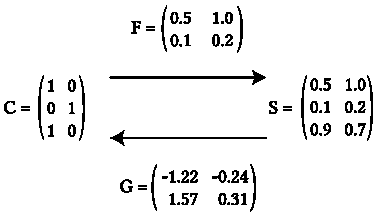
\includegraphics[width=200pt]{figures/fig3.1.pdf}
    \caption{Illustration of mapping between $C$ and $S$ matrix via $F$ (i.e. comprehension), and $S$ and $C$ matrix via $G$ (i.e. production). Note: In production, $C$ is referred to as $T$.}
    \label{fig:3_1}
\end{figure}

%\chapter{Production of word-final /s/}\label{chapter04}

As explained in detail in Section \ref{section02_1}, the present production study investigates the potential durational differences between three types of word-final /s/: non-morphemic /s/, plural /s/, and clitic /s/ (with the auxiliaries \textit{is} and \textit{has}).\footnote{An earlier version of this chapter has been published as part of \citet{Schmitz2021a}.} Pseudowords are used as items to prevent potential lexical effects to confound findings (see Section \ref{section03_1_1}). Three hypotheses derived from theories and models of speech production are examined. \textsc{H prod\textsubscript{1}}, the ``Feed-Forward Hypothesis", assumes that there is no durational difference between different types of word-final /s/. According to \textsc{H prod\textsubscript{2}}, the ``Prosodic Hypothesis", non-morphemic /s/ is shorter than plural /s/, and plural /s/ is shorter than auxiliary clitic /s/. \textsc{H prod\textsubscript{3}}, the ``Emergence Hypothesis", assumes that there are durational differences between different types of word-final /s/, but does not indicate what the nature of these durational differences is.

\section{Methodology}\label{section04_1}

\subsection{Speakers and recordings}\label{section04_1_1}

Forty native speakers of Southern British English took part in the experiment. Their mean age was 28.7 years, ranging from 19 to 58. Eight speakers were bi- or multilingual, and twenty-five speakers were from London while the other fifteen speakers were from other places in South Britain. None of the participants had a background in linguistics.

The recordings took place at Chandler House, University College London. The acoustic data were recorded on a computer with a Røde NT1-A microphone using an RME Fireface UC audio interface and sampled at 44.1 kHz, 16 bit.

\subsection{Materials}\label{section04_1_2}

For the production experiment, the pseudoword paradigm by \citet{Berko1958} was adopted. Following her reasoning, it was assumed that phonetic effects found in pseudoword paradigms mirror linguistic reality. The pseudowords used in the production experiment consist of the full set of pseudowords discussed in detail in Section \ref{section03_1_2}. For reasons of convenience, Table \ref{tab:4.1} lists these pseudowords once more.

\begin{table}\fontsize{10}{11}
\caption{Orthographic representations of all pseudowords.}
\label{tab:4.1}
\centering
\begin{tabular}{cccccc} 
\lsptoprule
gli-           & pru-           & plee-           & cloo-           & blou-           & glai-            \\ 
\midrule
\textit{glip}  & \textit{prup}  & \textit{pleep}  & \textit{cloop}  & \textit{bloup}  & \textit{glaip}   \\
\textit{glit}  & \textit{prut}  & \textit{pleet}  & \textit{cloot}  & \textit{blout}  & \textit{glait}   \\
\textit{glik}  & \textit{pruk}  & \textit{pleek}  & \textit{clook}  & \textit{blouk}  & \textit{glaik}   \\
\textit{glif}  & \textit{pruf}  & \textit{pleef}  & \textit{cloof}  & \textit{blouf}  & \textit{glaif}   \\ 
\midrule
\textit{glips} & \textit{prups} & \textit{pleeps} & \textit{cloops} & \textit{bloups} & \textit{glaips}  \\
\textit{glits} & \textit{pruts} & \textit{pleets} & \textit{cloots} & \textit{blouts} & \textit{glaits}  \\
\textit{gliks} & \textit{pruks} & \textit{pleeks} & \textit{clooks} & \textit{blouks} & \textit{glaiks}  \\
\textit{glifs} & \textit{prufs} & \textit{pleefs} & \textit{cloofs} & \textit{bloufs} & \textit{glaifs}  \\
\lspbottomrule
\end{tabular}
\end{table}

To elicit the pertinent types of /s/ under investigation, i.e. non-morphemic, plural, and \textit{is}- and \textit{has}-clitic /s/, 48 contexts and accompanying questions for /s/ elicitation were created. The verbs directly following the pseudowords in these contexts were chosen in such a way that out of twelve verbs in total, three each started with a voiceless plosive (/pl/, /k/), a vowel (/ɑ/, /i:/, /ʌ/, /eɪ/), a nasal (/m/, /n/), and an approximant (/w/, /l/, /r/). This was done to control for possible coarticulatory effects of these segmental classes with the preceding /s/. Examples are given in \ref{ex:4.1} to \ref{ex:4.4} with pseudowords and verbs in italics (see the supplementary material given in Chapter \ref{Supplementary Material} for all contexts).

\ex.
\label{ex:4.1}
Every day, the \textit{glips} \textit{plays} with the cloops.

\ex.
\label{ex:4.2}
Two days ago, the \textit{glips} \textit{ate} their lunch together.

\ex.
\label{ex:4.3}
Tonight, the \textit{glip's} \textit{meeting} the cloop for a drink.

\ex.
\label{ex:4.4}
The \textit{glip's} \textit{written} a love letter to the cloop.

To keep priming effects to a minimum, pseudowords were split into two groups. Each group consisted of 24 pseudowords, with 12 pseudowords used for morphemic /s/ elicitation and 12 pseudowords used for non-morphemic /s/ elicitation. This way it was ensured that no single participant encountered a phonologically identical pseudoword as both mono- and multi-morphemic, i.e. no participant was to encounter /glɪps/ as both singular and plural or clitic item. Participants were distributed equally across both groups. Each participant was supposed to produce 12 tokens for each of the four types of /s/ (non-morphemic, plural, \textit{is}-clitic, \textit{has}-clitic; 48 tokens overall).

To ensure that each pseudoword was elicited within each context, i.e. with each verb for each type of /s/, twelve pseudorandomised lists were created. The same twelve lists were used for both groups to keep them comparable. Additionally, types of /s/ were alternated in such a way that no type of /s/ was elicited twice in a row. This was done to keep priming effects to a minimum.

\subsection{Procedure}\label{section04_1_3}

First, participants were introduced to the idea of a recently discovered far away planet. They were told that the inhabitants of this planet at first might appear bizarre, but engage in activities known to the participants, and not to worry about the unfamiliar names of the creatures. Second, the trial structure was explained, i.e. for each slide there would be pictures and names of alien creatures, a short explanation of a situation, and a question relevant to the situation which was to be answered aloud. Participants were then told to proceed in a natural pace and to take as much time as necessary to read and understand the aliens’ names as well as the situations. To avoid possible confusion due to the simplicity of the task at hand, participants were made to believe that they were part of a control group of an experiment originally designed for children. Before starting practice trials, participants were reminded to use the aliens’ names instead of pronouns when answering. Then, a practice set of four contexts (see the supplementary material given in Chapter \ref{Supplementary Material}) was used to familiarise the participants with the experimental procedure itself.

\begin{figure}
    \centering
    \includegraphics[width=0.7\textwidth]{figures/fig4.1.png}
    \caption{Item, context, and question display during the production experiment.}
    \label{fig:4_1}
\end{figure}

For each trial, the screen proceeded similarly (see Figure \ref{fig:4_1} as well as examples \ref{ex:4.5} to \ref{ex:4.8}): First, the relevant pseudowords were introduced. In the stimuli testing the plural, one pseudoword (in its plural form) was introduced, while in the other three conditions two different pseudowords were introduced. In either case, two images (\cite{Vijver2014}) representing the pseudowords were used to create familiarity with the items under investigation. In all cases but plural, two images of different creatures were given, while in plural contexts two images of the same creature were used. The pseudowords and images were paired randomly across lists to rule out possible confounding effects of appearance, e.g. due to the \textit{bouba}/\textit{kiki} effect (e.g. \cite{Koehler1929, Fort2015}). Second, a context was introduced. Third, a question was given to elicit an answer with the pertinent type of /s/ while the context slowly faded out. The fading out of the question forced the participants not to rely on the reading-aloud of the given context. This open format was chosen in order to elicit speech that is as natural as possible. By choosing such an open format one obviously runs the risk of eliciting a large proportion of responses that do not contain the desired forms. This drawback of the experimental design was countered by having a large number of trials and participants. This strategy resulted in a sufficient number of observations. The experiment was carried out in a self-paced fashion; participants were instructed to progress in a contextually appropriate manner and at a speaking rate they considered to be normal.

\ex.
\label{ex:4.5}
non-morphemic context\\
\begin{blockarray}{ll}
\begin{block}{ll}
Introduction: & This is a glaits. \# And this is a pleeps.\\
Context: & Every day, the glaits plays with the pleeps.\\
Question: & What happens every day?\\
Answer: & The glaits plays with the pleeps.\\
\end{block}
\end{blockarray}

\ex.
\label{ex:4.6}
plural context\\
\begin{blockarray}{ll}
\begin{block}{ll}
Introduction: & This is a glait. \# And this is another one.\\
Context: & Two days ago, the glaits ate their lunch together.\\
Question: & What happened two days ago?\\
Answer: & The glaits ate their lunch together.\\
\end{block}
\end{blockarray}

\ex.
\label{ex:4.7}
\textit{is}-clitic context\\
\begin{blockarray}{ll}
\begin{block}{ll}
Introduction: & This is a glait. \# And this is a pleep.\\
Context: & Tonight, the glait’s meeting the pleep for a drink.\\
Question: & What’s happening tonight?\\
Answer: & The glait’s meeting the pleep for a drink.\\
\end{block}
\end{blockarray}

\ex.
\label{ex:4.8}
\textit{has}-clitic context\\
\begin{blockarray}{ll}
\begin{block}{ll}
Introduction: & This is a glait. \# And this is a pleep.\\
Context: & The glait’s written a love letter to the pleep.\\
Question: & What’s happened?\\
Answer: & The glait’s written a love letter to the pleep.\\
\end{block}
\end{blockarray}

\subsection{Labels and measurements}\label{section04_1_4}

In a first step, all recordings were manually transcribed on the utterance level. Using the freely available WebMAUS Basic system (\cite{Schiel1999, Kisler2017}), a phonetic transcription and segmentation based on the manual transcription was created. This automated segmentation was then manually checked by six trained annotators using the software Praat (\cite{Boersma2019}). Boundaries marking the beginning of an item or /s/ were moved to the nearest zero crossing where both spectrogram and waveform indicated the initiation of the gesture for the respective segment, following laid out segmentation criteria based on features of specific sounds as described in the phonetic literature (e.g. \cite{Ladefoged2003}). In the case of /s/, the boundaries were set to the zero crossing closest to the onset and offset of the friction visible in the waveform (see Figure \ref{fig:4_2}). If a pause followed the /s/, the boundary was set to the point where the friction of the /s/ dropped to silence. 

\begin{figure}
    \centering
    \includegraphics[width=1\textwidth]{figures/fig4.2.png}
    \caption{Example acoustic analysis of the item \textit{bloup’s}.}
    \label{fig:4_2}
\end{figure}

The reliability of the segmentation criteria was verified by trial segmentations, in which it was ensured that all annotators placed boundaries with only very small variations. Each annotator worked on a disjoint set of items; segmentation criteria were regularly re-verified in meetings of the annotators. After the segmentation process, a Praat script was used to extract the item, its phonetic transcription, and its duration, as well as the /s/ duration itself. If applicable, the duration of the following pause was also extracted. Additionally, the preceding and the following word were extracted as well.

\subsection{Pre-processing}\label{section04_1_5}

A part of the 1920 (40 participants × 48 utterances) recorded data points had to be excluded from analysis for one or more of the following reasons. If an utterance did not include a word-final /s/, this utterance was discarded (n = 599). A high number of failures to produce final /s/ was expected especially with the clitics since participants could use a different tense form, or the full form of the auxiliary. It was also expected that participants would produce wrong pronunciations (including those with the final /s/) of the newly encountered written word-forms, as the participants had to retrieve them from short-term memory after the fading out of the context. Additionally, utterances containing stutter or hesitation (n = 29) or replacement of pseudowords by pronouns (n = 15) were excluded as well. Some utterances were ungrammatical (n = 9), while other utterances contained pseudowords that were not part of the original set of pseudowords (n = 8). Cases where the interpretation of the final /s/ was ambiguous presented another problem (n = 114). An example of such a case is given in \ref{ex:4.9} where a \textit{has}-clitic was expected. Note that two pseudowords without a non-morphemic word-final /s/ were introduced, while either a non-morphemic /s/ or a \textit{has}-clitic /s/ was produced for the item under investigation, and most likely a non-morphemic word-final /s/ for the second pseudoword. As for regular inflected verbs there was no way to decide which type of /s/ had been produced in such cases, such utterances were discarded.

\ex.
\label{ex:4.9}
ambiguous case example\\
\begin{blockarray}{ll}
\begin{block}{ll}
Introduction: & This is a glait. \# And this is a pleep.\\
Context: & The glait’s attended concerts with the pleep \\
~ & many times.\\
Question: & What’s happened many times?\\
Answer: & The glaits attended many concerts with the pleeps \\
~ & many times. \\
\end{block}
\end{blockarray}

After exclusions, 1146 data points (approx. 60\%) remained in the final data set. The final data set as well as the analysis and results discussed in the following sections can be found in the supplementary material given in Chapter \ref{Supplementary Material}.

\section{Analysis}\label{section04_2}

\subsection{Covariates}\label{section04_2_1}

The set of covariates chosen for the present study is similar to that of other studies on phonetic effects of morphological structure (\cite{Pluymaekers2005a, Pluymaekers2005b, Hanique2013Ernestus, Plag2017}). In the following, covariates used as fixed effects are described first. Then, variables used as random effects are introduced.

\textsc{baseDurLog}. Indicating a more local speaking rate (e.g. \cite{Plag2017}), base duration was measured. Base duration in this case is equal to the summed duration of all word-internal segments preceding the /s/ under investigation. That is, the base of multi-morphemic items and the segmental string without the final /s/ of mono-morphemic items is henceforth considered the base. The base duration was log-transformed and centred (\cite{Robinson2009, Afshartous2011, Winter2019}). This variable is called \textsc{baseDurLog}.

\textsc{biphoneProb}. A potential problem with using pseudowords is their phonotactics. Pseudowords created for this book are mostly phonotactically legal (see Section \ref{section03_1_2} and the relevant footnote therein), and their final consonant clusters (with /s/ as the second consonant) are not uncommon in multi-morphemic words. However, in mono-morphemic words these clusters are rarer, or, in the case of /fs/, even unattested (e.g. in CELEX, \cite{Baayen1995}). The different phonotactic probabilities of these clusters could potentially influence the pronunciation of /s/ in the pseudowords, especially when spoken in the contexts where these words receive a mono-morphemic interpretation. To address this concern, the probability of the final biphones /fs/ ($0$), /ks/ ($0.00427$), /ps/ ($0.00058$), and /ts/ ($0.00072$) in mono-morphemic words was included as a covariate. \textsc{biphoneProb} was computed on the basis of the transcriptions of all mono-morphemic words in CELEX.

\textsc{biphoneProbSum} \& \textsc{biphoneProbSumBin}. A potential factor influencing the duration of a word in running speech is its predictability in context. The more predictable, the shorter the duration (\cite{Pluymaekers2005a, Bell2009, Torreira2009}). Such a word bigram frequency, however, is not applicable to pseudowords for obvious reasons. Instead, the summed biphone probability was used analogously as a comparable measure. The summed biphone probability for each pseudoword and its phonological variants was calculated using the Phonotactic Probability Calculator (\cite{Vitevitch2004}). Additionally, a binary covariate based on the summed biphone probability was created. The threshold for low versus high summed biphone probability for \textsc{biphoneProbSumBin} was the mean of the continuous covariate. That is, all values below the mean were considered to be low, while all values above the mean were taken as high.

\textsc{folSeg} \& \textsc{folType}. To account for potential effects of the following word on the duration of /s/ (cf. \cite{Klatt1976, Umeda1977}), these were included in regard to their onset segment adjacent to the word-final /s/. This segment was included in its phonological representation in \textsc{folSeg} (e.g. \texttt{k} for the onset of \textit{cooked}) as well as in its segmental class by \textsc{folType} (i.e. approximant \texttt{APP} for \textit{listen}, fricative \texttt{F} for \textit{find}, nasal \texttt{N} for \textit{know}, plosive \texttt{P} for \textit{cook}, vowel \texttt{V} for \textit{eat}).

\textsc{gender} / \textsc{location} / \textsc{monoMultilingual}. Participants’ \textsc{gender} and whether they had grown up in London or elsewhere in South Britain (\textsc{location}) were included as well as they may influence phonetic realisations. Additionally, participants who were early bilinguals (i.e. the L2 was/the L2s were acquired as a pre-school child) were categorised as multilingual, while all other participants were categorised as monolingual in \textsc{monoMultilingual}.\footnote{Psycholinguistic experiments are standardly done with monolingual speakers (mostly of English, and mostly in the US). In the multicultural context of a large European city like London, experiments with student populations necessarily involve speakers that are multilingual (with varying degrees of competence). To control for this potential confound, the variable \textsc{monoMultilingual} was added. While there are studies of phonetic duration in bilingual speech (e.g. \cite{Mack1982, Lee2012}) the effect of mono-/multilingualism on the duration of word-final /s/ has not been explored yet.}

\textsc{neighbourhoodDensity} \& \textsc{neighbourhoodFrequency}. The densities and frequencies of neighbourhoods were included as covariates as the number of neighbours may influence phonetic reduction (e.g. \cite{Gahl2012}). Both neighbourhood measures were taken from the CLEARPOND database (\cite{Marian2012}). That is, \textsc{neighbourhoodDensity} describes the number of words differing in one segment from the item in question (\cite[3]{Marian2012}), while \textsc{neighbourhoodFrequency} describes the mean frequency (per million) of these neighbouring words.

\textsc{pauseDur} \& \textsc{pauseBin}. In order to account for final-lengthening effects, all stretches of silence between the offset of the word-final /s/ and the onset of the following word were measured. Silence of 50 ms and above was considered as pause (\cite{Lee1999}; see also \cite{Zvonik2003} and \cite{Krivokapic2007} on short pause duration in between short phrases). The closure durations of following plosives were taken into account by subtracting the mean closure duration of the pertinent plosive (mean values for /p, t, k/ adopted from \cite{Yao2007}) from the measured stretch of silence. It was considered a pause only if the resulting duration was above the aforementioned threshold. Pause measurements were included as the continuous variable \textsc{pauseDur} as well as the binary variable \textsc{pauseBin} (with the levels \texttt{pause} and \texttt{no\_pause}).

\textsc{preC}. It has been shown that the consonant preceding word-final /s/ may influence the duration of word-final /s/ (e.g. \cite{Umeda1977}). In particular, \citet[853]{Umeda1977} finds that /s/ becomes shorter after plosives, and longer after the fricative /θ/ (and this presumably also holds for /s/ after the fricative /f/). The consonant preceding the final /s/ was therefore included as a covariate, \textsc{preC}.

\textsc{speakingRate}. As speaking rate is a self-evident variable affecting segment durations, this was controlled for. The speaking rate was computed as the number of syllables in an utterance divided by the duration of the utterance. For the statistical analysis, \textsc{speakingRate} was centred (\cite{Robinson2009, Afshartous2011, Winter2019}). The computation was done automatically in Praat (\cite{deJong2008}). This way of computing speaking rate is similar to that utilised in previous studies (e.g. \cite{Plag2017}).

\textsc{item} \& \textsc{transcription}. Pseudowords were sometimes produced with varying segmental make-up. Therefore, both the orthographic representation of the pseudoword and a phonological transcription of the word as spoken were included as variables. These covariates were labelled \textsc{item} and \textsc{transcription}.

\textsc{list} \& \textsc{slideNumber}. To account for possible durational differences due to priming and similar effects, the list number (1 to 12) and the point of occurrence during the experiment of the individual item were also included.

\textsc{speaker} / \textsc{age}. \textsc{speaker} ID was included to account for inter-speaker differences in production. \textsc{age} was included as well, as it may show an influence on phonetic realisations.

\subsection{Overview of the data}\label{section04_2_2}

An overview of all variables and their distribution is given in Table \ref{tab:4.2} and Table \ref{tab:4.3}.

\begin{table}\fontsize{10}{11}
\caption{Summary of categorical predictors and the explanatory variable of interest in the final data set.}
\label{tab:4.2}
\centering
\begin{tabular}{ll}
\lsptoprule
Categorical predictors                & Levels                                                   \\
\midrule
\textsc{item}                                  & 48                                                       \\
\textsc{transcription}                         & 67                                                       \\
\multirow{2}{*}{\textsc{NeighbourhoodDensity}} & \texttt{0}: 419

~ ~~

\texttt{1}: 238~ ~ ~ \texttt{2}: 165~ ~ ~ \texttt{3}: 107             \\
                                      & \texttt{4}: 14~ ~ ~ \texttt{5}: 114~ ~ ~ \texttt{6}: 32~ ~ ~ \texttt{7}: 30                  \\
\textsc{pauseBin}                              & \texttt{no}: 777~ ~ ~ \texttt{yes}: 342                                    \\
\textsc{biphoneProbSumBin}                     & \texttt{low}: 856~ ~ ~ \texttt{high}: 263                                  \\
\textsc{list}                                  & 24                                                       \\
\textsc{slideNumber}                           & 48                                                       \\
\textsc{preC}                                  & \texttt{f}: 273~ ~ ~ \texttt{k}: 292~ ~ ~ \texttt{p}: 281~ ~ ~ \texttt{t}: 273               \\
\textsc{folSeg}                                & 18                                                       \\
\textsc{folType}                               & \texttt{APP}: 229~ ~ ~ \texttt{F}: 12~ ~ ~ \texttt{N}: 230~ ~ ~ \texttt{P}: 300~ ~ ~ \texttt{V}: 278  \\
\textsc{speaker}                               & 40                                                       \\
\textsc{gender}                                & 2                                                        \\
\textsc{location}                              & \texttt{London}: 636~ ~ ~ \texttt{elsewhere}: 483                          \\
\textsc{monoMultilingual}                      & \texttt{monolingual}: 871~ ~ ~ \texttt{multilingual}: 248                  \\
\midrule
Explanatory variable                  & Levels                                                   \\
\midrule
\textsc{typeOfS}                               & \texttt{nm}: 308~ ~ ~ \texttt{pl}: 373~ ~ ~ \texttt{is}: 284~ ~ ~ \texttt{has}: 154   \\      
\lspbottomrule
\end{tabular}
\end{table}



\begin{table}\fontsize{10}{11}
\caption{Summary of the dependent variable and numerical predictors in the final data set.}
\label{tab:4.3}
\centering
\begin{tabular}{lrrrr} 
\lsptoprule
Dependent variable     & Mean   & St. Dev. & Min        & Max      \\ 
\midrule
\textsc{sDurLog}                & 0.002  & 0.388    & -
  1.201~ & 1.098~   \\ 
\midrule
Numerical predictors   & Mean   & St. Dev. & Min        & Max      \\ 
\midrule
\textsc{speakingRate}           & -0.000 & 0.899    & 2.250      & 3.540    \\
\textsc{baseDurLog}             & 0.072  & 0.194    & 0.000      & 3.559    \\
\textsc{pauseDur}               & 0.072  & 0.193    & 0.000      & 3.559    \\
\textsc{neighbourhoodFrequency} & 27.345 & 84.645   & 0.000      & 412.027  \\
\textsc{biphoneProbSum}         & 0.013  & 0.007    & 0.005      & 0.031    \\
\textsc{biphoneProb}            & 0.001  & 0.002    & 0.000      & 0.004    \\
\textsc{age}                    & 28.740 & 9.743    & 19.000     & 58.000   \\
\lspbottomrule
\end{tabular}
\end{table}


\subsection{Collinearity}\label{section04_2_3}

As described in Section \ref{section03_2_3}, one issue to address when fitting a model to a multitude of similar covariates is collinearity (e.g. \cite{Tomaschek2018collin}). To avoid such issues, covariates were tested for correlation issues. High correlation coefficients, i.e. $|rho|≥0.5$, were found for \textsc{item} and \textsc{transcription} ($rho=0.82,$ $p<0.001$, Spearman), \textsc{pauseDur} and \textsc{pauseBin} ($rho=0.87,p<0.001$, Spearman), \textsc{neighbourhoodDensity} and \textsc{neighbourhoodFrequency} ($rho=0.86,$ $p<0.001$, Spearman), \textsc{biphoneProbSum} and \textsc{biphoneProbSumBin} ($rho=0.87,$ $p<0.001$, Spearman), and for \textsc{folSeg} and \textsc{folType} ($rho=-0.74,p<0.001$, Spearman).    

Given the nature of the highly correlated variable pairs, that is both variables tap into very similar features of the given items or utterances, it was decided to make use of the competitive exclusion strategy outlined in Section \ref{section03_2_3}. This procedure led to the exclusion of \textsc{item} (in favour of \textsc{transcription}), \textsc{pauseDur} (in favour of \textsc{pauseBin}), \textsc{neighbourhoodFrequency} (in favour of \textsc{neighbourhoodDensity}), \textsc{biphoneProbSum} (in favour of \textsc{biphoneProbSumBin}), \textsc{folSeg} (in favour of \textsc{folType}), and \textsc{biphoneProb} (in favour of \textsc{preC}).

\subsection{Statistical analysis}\label{section04_2_4}

Differences in consonant duration may play out as differences in absolute duration or as differences in relative duration (e.g. with gemination: \cite{Oh2012, Ridouane2017, BenHedia2019}). Some previous analyses of the duration of /s/ (\cite{Plag2017}) have therefore looked at both absolute and relative duration, and the present study will also present these two types of analyses. In the first analysis (Section \ref{section04_3_1}) absolute duration of /s/ was used as the dependent variable, whereas in the second analysis (Section \ref{section04_3_2}) the duration of /s/ relative to the duration of the whole word was used as the dependent variable. Relative duration (i.e. the variable \textsc{proportionOfS}) was calculated by dividing the absolute duration of the /s/ by the duration of the whole word. 

The dependent variable, duration of /s/, was log-transformed and centred following standard procedures to reduce the potentially harmful effect of skewed distributions in linear regression models (e.g. \cite{Winter2019}). The name of this variable is \textsc{sDurLog}. \textsc{proportionOfS} did not have a skewed distribution and no transformation was necessary. Following the modelling procedure for LMER models outlined in Section \ref{section03_2_1}, models for \textsc{sDurLog} and \textsc{proportionOfS} as dependent variables were fitted, tested for collinearity issues by using variance inflation factors, and finally trimmed. This resulted in a loss of 9 data points (0.8\%) for \textsc{sDurLog} and in a loss of 12 data points (1.0\%) for \textsc{proportionOfS}, and in both cases led to a satisfactory distribution of the residuals.

\section{Results}\label{section04_3}

\subsection{Absolute duration}\label{section04_3_1}

Figure \ref{fig:4_3} shows the distribution of the observed durations of non-morphemic, plural, \textit{is}-, and \textit{has}-clitic /s/. On average, non-morphemic /s/ duration is 134 ms, which is about 13 ms longer than plural /s/ with a mean duration of 121 ms. The mean duration of the \textit{is}-clitic is 103 ms and the mean duration of the \textit{has}-clitic is 94 ms. 

\begin{figure}
    \centering
    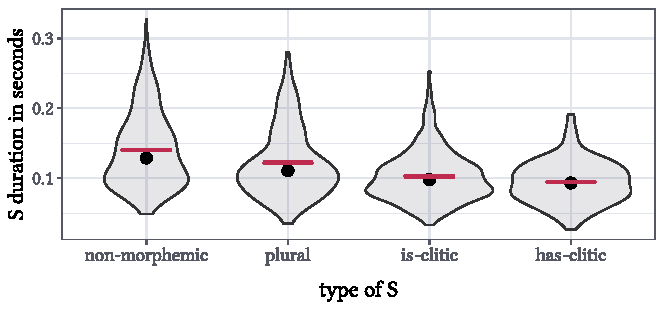
\includegraphics[]{figures/fig4.3.pdf}
    \caption{Observed durations of non-morphemic, plural, \textit{is}- and \textit{has}-clitic /s/. The dot represents the median, the horizontal line indicates the mean. The violin shapes represent rotated density plots describing the distribution of the data.}
    \label{fig:4_3}
\end{figure}

Multivariate analyses as described in the previous section were then conducted to control for the many potentially intervening influences of the described covariates listed in Section \ref{section04_2_1}. In the final model, fitted according to the procedure described above, main effects of type of /s/ (\textsc{typeOfS}), speaking rate (\textsc{speakingRate}), base duration (\textsc{baseDurLog}), pause (\textsc{pauseBin}), preceding consonant (\textsc{preC}), biphone probability sum (\textsc{biphoneProbSumBin}), following segmental type (\textsc{fol-Type}), and mono-/multilingualism (\textsc{monoMultilingual}) were found.

Regarding the random effects, only \textsc{speaker}-specific random intercepts turned out to significantly improve the model fit. The \textit{p}-values for the analysis of variance of the final model are given in Table \ref{tab:4.4}.

\begin{table}\fontsize{10}{11}
\caption{\textit{p}-values of fixed effects in the final model, fitted to the log-transformed durations of /s/.}
\label{tab:4.4}
\centering
\begin{tabular}{lrrrrrr} 
\lsptoprule
~                 & Sum Sq & Mean Sq & NumDF & DenDF   & F.value & Pr ( F)  \\ 
\midrule
\textsc{typeOfS}           & 5.312  & 1.771   & 3     & 1089.66 & 33.338  & 0.000    \\
\textsc{speakingRate}      & 0.230  & 0.230   & 1     & 1117.09 & 4.324   & 0.038    \\
\textsc{baseDurLog}        & 9.466  & 9.466   & 1     & 1079.58 & 178.220 & 0.000    \\
\textsc{pauseBin}          & 6.970  & 6.970   & 1     & 1110.28 & 131.235 & 0.000    \\
\textsc{biphoneProbSumBin} & 0.398  & 0.398   & 1     & 1082.26 & 7.492   & 0.006    \\
\textsc{preC}              & 0.623  & 0.208   & 3     & 1080.29 & 3.910   & 0.009    \\
\textsc{folType}           & 2.677  & 0.669   & 4     & 1081.55 & 12.598  & 0.000    \\
\textsc{monoMultilingual}  & 0.345  & 0.345   & 1     & 37.37   & 6.498   & 0.015    \\
\lspbottomrule
\end{tabular}
\end{table}

The final model was then analysed in terms of its R\textsuperscript{2} values which were computed with the \texttt{MuMIn} package (\cite{Barton2020}; for marginal and conditional R\textsuperscript{2} value computation, see \cite{Nakagawa2017}). The marginal R\textsuperscript{2} value of a model indicates the percentage of variation in the data explained by the fixed effects of that model. The variance explained by the entire model is given by its conditional R\textsuperscript{2} value. The marginal R\textsuperscript{2} value of the model is $0.46$, that is, fixed effects explain 46\% of the variation in the data. The variance explained by the entire model is 61\% as obtained by the conditional R\textsuperscript{2} value of $0.61$.

The estimates of the final model and their \textit{p}-values are given in Table \ref{tab:4.5}. The reference levels for the categorical predictors are: for \textsc{typeOfS} it is \texttt{non-morphemic} /s/, for \textsc{pauseBin} it is \texttt{no-pause}, for \textsc{biphoneProbSumBin} it is \texttt{low}, for \textsc{preC} it is \texttt{t}, for \textsc{folType} it is \texttt{approximant}, and for \textsc{monoMultilingual} it is \texttt{monolingual}. All coefficients can be interpreted as changes relative to these reference levels.

\begin{table}\fontsize{10}{11}
\caption{Fixed-effect coefficients and \textit{p}-values as computed by the final model (mixed-effects model fitted to the log-transformed and centred durations of /s/).}
\label{tab:4.5}
\centering
\begin{tabular}{lrrrrr} 
\lsptoprule
~                            & Estimate & SE    & df      & \textit{t}-value & Pr(\textbar{}t\textbar{})  \\ 
\midrule
(Intercept)                  & -1.321   & 0.068 & 550.378 & -19.498          & 0.000                      \\
\textsc{typeOfS}\texttt{pl}                    & -0.114   & 0.019 & 1094.00 & -6.062           & 0.000                      \\
\textsc{typeOfS}\texttt{is}                    & -0.178   & 0.020 & 1096.00 & -8.839           & 0.000                      \\
\textsc{typeOfS}\texttt{has}                   & -0.196   & 0.024 & 1091.00 & -8.140           & 0.000                      \\
\textsc{speakingRate}                 & -0.021   & 0.010 & 1117.00 & -2.079           & 0.038                      \\
\textsc{baseDurLog}                   & 0.586    & 0.044 & 1080.00 & 13.35            & 0.000                      \\
\textsc{pauseBin}\texttt{pause}                & 0.206    & 0.018 & 1110.00 & 11.456           & 0.000                      \\
\textsc{biphoneProbSumBin}\texttt{high}        & 0.047    & 0.017 & 1082.00 & 2.737            & 0.006                      \\
\textsc{preC}\texttt{f}                        & 0.061    & 0.020 & 1081.00 & -3.044           & 0.003                      \\
\textsc{preC}\texttt{k}                        & 0.055    & 0.020 & 1082.00 & -0.303           & 0.006                      \\
\textsc{preC}\texttt{p}                        & 0.050    & 0.020 & 1079.00 & 2.522            & 0.012                      \\
\textsc{folType}\texttt{F}                     & 0.012    & 0.070 & 1084.00 & 0.171            & 0.864                      \\
\textsc{folType}\texttt{N}                     & -0.036   & 0.021 & 1079.00 & -1.764           & 0.078                      \\
\textsc{folType}\texttt{P}                     & -0.045   & 0.019 & 1080.00 & -2.384           & 0.017                      \\
\textsc{folType}\texttt{V}                     & -0.136   & 0.020 & 1082.00 & -6.85            & 0.000                      \\
\textsc{monoMultilingual}\texttt{multilingual} & -0.152   & 0.059 & 37.37   & -2.549           & 0.015                      \\
\lspbottomrule
\end{tabular}
\end{table}

The predictor strength of individual predictors was checked following the method outlined in Section \ref{section03_2_1}, that is by fitting models that lacked a particular predictor and comparing their marginal R\textsuperscript{2} values to those of the final model. The results are reflected in the hierarchy given in \ref{ex:4.10}. The decrease in R\textsuperscript{2} is greatest when removing \textsc{baseDurLog}, followed by \textsc{pauseBin}, and so forth. Overall, the morphological status of an /s/ appears to be a strong predictor of its acoustic duration.

\ex.
\label{ex:4.10}
\textsc{baseDurLog >> pauseBin >> typeOfS >> monoMultilingual >> folType >> speakingRate >> biphoneProbSumBin >> PreC}

Figure \ref{fig:4_4} shows the effect of the numerical variables included in the final model on /s/ duration. The estimated values of the dependent variable and the base duration are back-transformed into seconds. Speaking rate and base duration show effects in the expected direction. With faster speech, /s/ becomes shorter (Panel A), while longer base durations also come with longer /s/ durations (Panel B). 

\begin{figure}
    \centering
    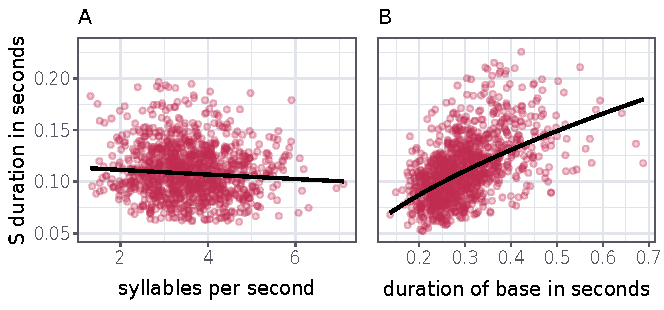
\includegraphics[width=1\textwidth]{figures/fig4.4.pdf}
    \caption{Partial effects of the numerical variables \textsc{speakingRate} (Panel A) and \textsc{baseDurLog} (back-transformed, Panel B) included in the final model, fitted to the log-transformed values of duration of /s/.}
    \label{fig:4_4}
\end{figure}


The partial effects of the categorical variables included in the final model are illustrated in Figure \ref{fig:4_5}. /s/ duration is longer if the /s/ is followed by a pause (Panel A), which can be interpreted as a clear case of phrase-final lengthening (e.g. \cite{Cooper1981}). Higher biphone probability sum leads to longer /s/ durations (Panel B). There is also an effect of the preceding consonant: The plosive /t/ is followed by significantly shorter /s/ durations than are /k/ and /f/ (Panel C). /s/ duration is significantly shorter when followed by a vowel, while all other differences between following consonants are minor in nature (Panel D). Lastly, monolingual speakers produce longer /s/ durations than multilingual speakers (Panel E).

\begin{figure}
    \centering
    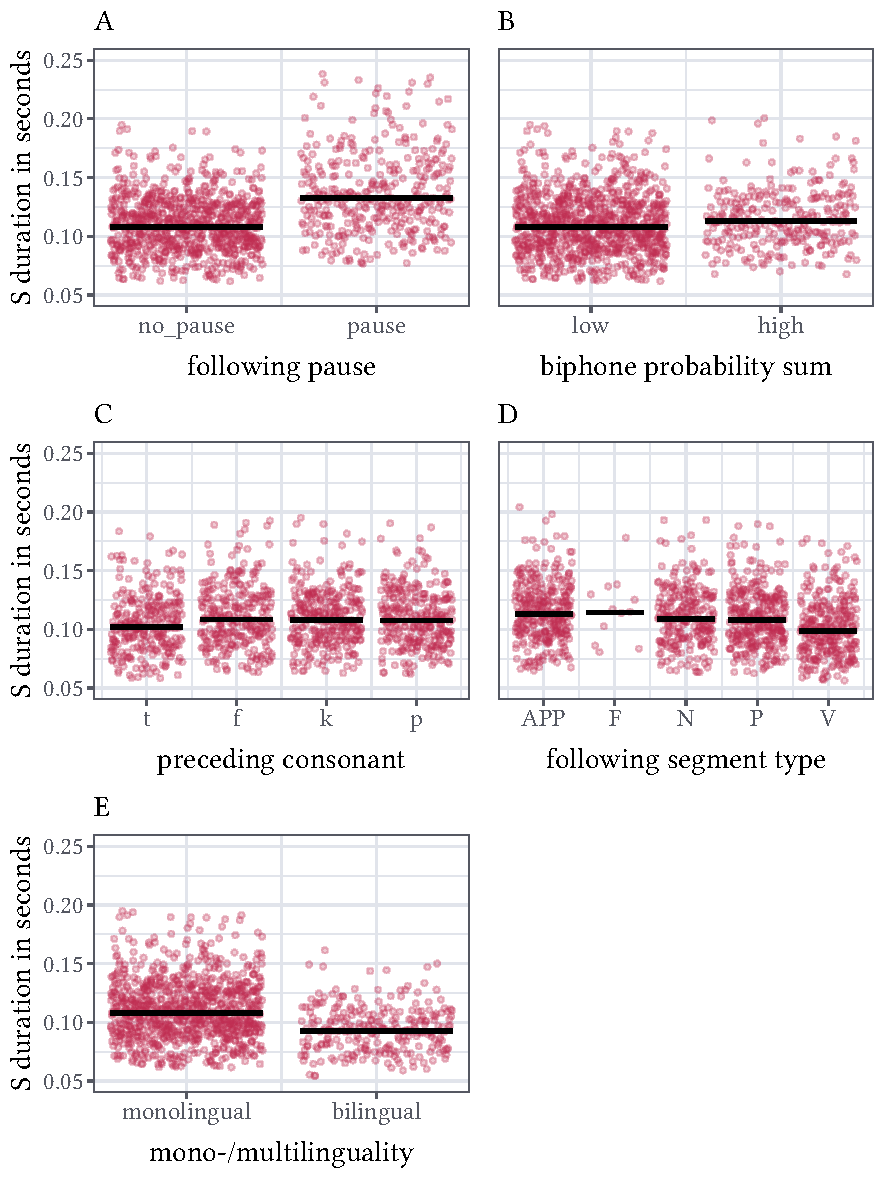
\includegraphics[]{figures/fig4.5.pdf}
    \caption{Partial effects of the categorical variables \textsc{pauseBin} (Panel A), \textsc{biphoneProbSumBin} (Panel B), \textsc{preC} (Panel C), \textsc{folType} (Panel D), and \textsc{monoMultilingual} (Panel E) included in the final model, fitted to the log-transformed values of duration of /s/.}
    \label{fig:4_5}
\end{figure}

The effect of the variable of interest, i.e. \textsc{typeOfS}, is plotted in Figure \ref{fig:4_6}. As above, the values of the dependent variable are back-transformed into seconds.

\begin{figure}
    \centering
    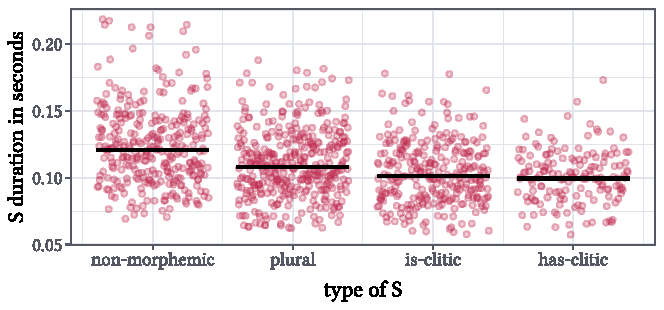
\includegraphics[width=1\textwidth]{figures/fig4.6.pdf}
    \caption{Partial effect of \textsc{typeofS} in the final model, fitted to the log-transformed values of duration of /s/.}
    \label{fig:4_6}
\end{figure}

One can see that there are durational differences between the different types of /s/. The results of pair-wise comparisons of the predicted means using Tukey contrasts (as implemented by the \texttt{SfL} package, \cite{Schmitz2021sfl}) are summarised in Table \ref{tab:4.6}.

\begin{table}\fontsize{10}{11}
\caption{Multiple comparisons of means of duration of /s/ (Tukey contrasts). Significance codes: `***' $p < 0.001$, `**' $p < 0.01$, `*' $p < 0.05$.}
\label{tab:4.6}
\centering
\begin{tabular}{llllrrrr} 
\lsptoprule
~                   & ~ & ~                  & Estimate & SE    & \textit{z}-value & Pr(\textbar{}z\textbar{}) & ~    \\ 
\midrule
plural              & - & non-morphemic      & -0.114   & 0.019 & -6.062           & 
  0.001                  & ***  \\
\textit{is}-clitic  & - & non-morphemic      & -0.188   & 0.020 & -8.839           &  0.001                    & ***  \\
\textit{has}-clitic & - & non-morphemic      & -0.196   & 0.024 & -8.140           & 
  0.001                  & ***  \\
\textit{is}-clitic  & - & plural             & -0.064   & 0.019 & -3.294           & 0.005                     & **   \\
\textit{has}-clitic & - & plural             & -0.082   & 0.023 & -3.503           & 0.003                     & **   \\
\textit{has}-clitic & - & \textit{is}-clitic & -0.018   & 0.023 & -0.766           & 0.868                     & ~    \\
\lspbottomrule
\end{tabular}
\end{table}

Based on the Tukey tests, the comparison of the different types of /s/ yields the significant contrasts shown in Table \ref{tab:4.7}. Considering the different durations given in Table \ref{tab:4.8}, the following hierarchy emerges: non-morphemic /s/ > plural /s/ > \textit{is}-/\textit{has}-clitic /s/.

\begin{table}\fontsize{10}{11}
\caption{Significant contrasts in duration between different types of /s/. Significance codes: `***' $p < 0.001$, `**' $p < 0.01$, `*' $p < 0.05$.}
\label{tab:4.7}
\centering
\begin{tabular}{lrrrr} 
\lsptoprule
~                   & nm   & pl   & \textit{is} & \textit{has}  \\ 
\midrule
non-morphemic       & n.a. & ***  & ***         & ***           \\
plural              & ~    & n.a. & **          & **            \\
\textit{is}-clitic  & ~    & ~    & n.a.        & ~             \\
\textit{has}-clitic & ~    & ~    & ~           & n.a.          \\
\lspbottomrule
\end{tabular}
\end{table}



\begin{table}\fontsize{10}{11}
\caption{/s/ durations as estimated by the final model using non-centred data. All values are back-transformed to seconds. Values given are estimated for items without following pause, high biphone sum probability, monolingual speakers, and across all preceding and following segment types.}
\label{tab:4.8}
\begin{tabular}{lr} 
\lsptoprule
\textsc{typeOfS}                      & Mean   \\ 
\midrule
non-morphemic                & 0.224  \\
plural                       & 0.200  \\
\textit{is}-clitic           & 0.187  \\
\textit{has}-clitic          & 0.184  \\
\lspbottomrule
\end{tabular}
\end{table}

To summarise, the durational differences between non-morphemic and other types of /s/, as well as the durational difference between plural and the clitics are significant, while there is no significant durational difference between the two clitics. Non-morphemic /s/ is longest in duration, followed by plural /s/, which in turn is followed by clitic /s/.

\subsection{Relative duration}\label{section04_3_2}

The results for relative duration are very similar to those of absolute duration. The \textit{p}-values for the analysis of variance of the final model are given in Table \ref{tab:4.9}. Table \ref{tab:4.10} shows the coefficients for the final model. All effects go in the same direction as in the analysis of absolute duration. The only predictors that have lost significance when compared to the model for absolute duration are \textsc{preC} and \textsc{speakingRate}. The differences in the means show the same pattern as in the analysis of absolute duration, as can be seen in Table \ref{tab:4.11}.

\begin{table}\fontsize{10}{11}
\caption{\textit{p}-values of fixed effects in the final model, fitted to the relative durations of /s/.}
\label{tab:4.9}
\centering
\begin{tabular}{lrrrrrr} 
\lsptoprule
~                 & Sum Sq & Mean Sq & NumDF & DenDF   & F.value & Pr(F)  \\ 
\midrule
\textsc{typeOfS}           & 0.161  & 0.054   & 3     & 1070.68 & 25.510  & 0.000  \\
\textsc{pauseBin}          & 0.186  & 0.186   & 1     & 1101.26 & 88.518  & 0.000  \\
\textsc{biphoneProbSumBin} & 0.015  & 0.015   & 1     & 36.32   & 6.917   & 0.012  \\
\textsc{folType}           & 0.071  & 0.018   & 4     & 1063.31 & 8.389   & 0.000  \\
\textsc{monoMultilingual}  & 0.010  & 0.010   & 1     & 37.81   & 4.561   & 0.039  \\
\lspbottomrule
\end{tabular}
\end{table}




\begin{table}\fontsize{10}{11}
\caption{Fixed-effect coefficients and \textit{p}-values as computed by the final model (mixed-effects model fitted to the relative durations of /s/).}
\label{tab:4.10}
\centering
\begin{tabular}{lrrrrr} 
\lsptoprule
~                            & Estimate & SE    & df      & \textit{t}-value & Pr(\textbar{}t\textbar{})  \\ 
\midrule
(Intercept)                  & 0.299    & 0.007 & 89.73   & 45.827           & 0.000                      \\
\textsc{typeOfS}\texttt{pl}                    & -0.019   & 0.004 & 1085.00 & -5.157           & 0.000                      \\
\textsc{typeOfS}\texttt{is}                    & -0.031   & 0.004 & 1070.00 & -7.651           & 0.000                      \\
\textsc{typeOfS}\texttt{has}                   & -0.035   & 0.005 & 1067.00 & -7.260           & 0.000                      \\
\textsc{pauseBin}\texttt{pause}                & 0.033    & 0.004 & 1101.00 & 9.408            & 0.000                      \\
\textsc{biphoneProbSumBin}\texttt{high}        & 0.013    & 0.005 & 36.32   & 2.630            & 0.012                      \\
\textsc{folType}\texttt{F}                     & 0.001    & 0.014 & 1068.00 & 0.086            & 0.931                      \\
\textsc{folType}\texttt{N}                     & -0.006   & 0.004 & 1061.00 & -1.409           & 0.159                      \\
\textsc{folType}\texttt{P}                     & -0.007   & 0.004 & 1056.00 & -1.708           & 0.088                      \\
\textsc{folType}\texttt{V}                     & -0.022   & 0.004 & 1063.00 & -5.568           & 0.000                      \\
\textsc{monoMultilingual}\texttt{multilingual} & -0.024   & 0.011 & 37.81   & -2.136           & 0.039                      \\
\lspbottomrule
\end{tabular}
\end{table}




\begin{table}\fontsize{10}{11}
\caption{Multiple comparisons of means of duration of /s/ (Tukey contrasts). Significance codes: `***' $p < 0.001$, `**' $p < 0.01$, `*' $p < 0.05$.}
\label{tab:4.11}
\centering
\begin{tabular}{lllrrrrr} 
\lsptoprule
~                   & ~ & ~                  & Estimate & SE    & \textit{z}-value & Pr(\textbar{}z\textbar{}) & ~    \\ 
\midrule
plural              & - & non-morphemic      & -0.019   & 0.004 & -5.157           & 
  0.001                  & ***  \\
\textit{is}-clitic  & - & non-morphemic      & -0.031   & 0.004 & -7.651           &  0.001                    & ***  \\
\textit{has}-clitic & - & non-morphemic      & -0.035   & 0.005 & -7.260           & 
  0.001                  & ***  \\
\textit{is}-clitic  & - & plural             & -0.011   & 0.004 & -2.936           & 0.017                     & *    \\
\textit{has}-clitic & - & plural             & -0.015   & 0.005 & -3.300           & 0.005                     & **   \\
\textit{has}-clitic & - & \textit{is}-clitic & -0.004   & 0.005 & -0.854           & 0.827                     & ~    \\
\lspbottomrule
\end{tabular}
\end{table}



\section{Discussion}\label{section04_4}

Following in the footsteps of previous studies on durational differences between different types of /s/, this study tested whether the morphological category of word-final /s/ has an influence on its acoustic duration in speech production. In order to avoid imbalanced data as in the case of corpus studies, speech material elicited by the means of highly controlled contexts of a production task was used. For the first time in this context, pseudowords instead of real words were used to minimise potentially confounding lexical effects. It was found that there are significant durational differences between non-morphemic and morphemic types of word-final /s/, with morphemic types of /s/ being significantly shorter in duration than non-morphemic /s/. Also, there are significant durational differences between the plural suffix and the \textit{is}- and \textit{has}-clitic /s/, with plural /s/ being significantly longer than clitic /s/ and with no significant difference between the two clitics. Hence, the type of /s/ emerged as a strong, significant predictor of segmental duration.

The differences between different types of /s/ in the present study are completely in line with previous studies that were based on speech corpora and on different varieties of English (\cite{Plag2017} and \cite{Tomaschek2019} on North American English; \cite{Zimmermann2016} on New Zealand English). In those studies the same pattern of differences was found. Turning to previous experimental studies, differing results are found. The results of both prior experimental studies (\cite{Walsh1983, Seyfarth2017}) are subject to potentially confounding effects of the lexical and contextual properties of the items under investigation. Their finding of non-morphemic /s/ being shorter than morphemic /s/ may well be an artefact of such properties. The items used in the present study, however, are much less prone to be subject to such effects as they are pseudowords with no established representations in the speakers’ mental lexicons. The results on the duration of clitic /s/ cannot be compared to previously reported ones by other experimental studies, as none of the previously conducted experimental studies investigated clitic /s/ production.

No previous studies have used pseudowords either, so before turning to the theoretical interpretation of the results of the present study, a few words are in order on whether using pseudowords might have had an undesired impact on the results. While the use of pseudowords in phonetic experiments comes with a number of benefits (see Section \ref{section03_1_1}), it also raises some questions. First, there is the issue of phonotactic probability raised in Section \ref{section04_2_1}. Two measures concerned with phonotactics (one describing the phonotactic probability of the whole word, the other taking into consideration the consonant preceding the word-final /s/) were included in the statistical analysis to address this issue. It turned out that phonotactic probability influences the production of pseudowords, as it does for real words. Crucially, there was no interaction between the type of /s/ and the consonant preceding it in mono-morphemic words. This means that speakers produced these clusters in the same way, no matter whether the cluster occurred in the mono-morphemic words or whether the cluster straddled the morphemic boundary between the base and the /s/. The main effects of the phonotactic variables turned out to be rather weak and, crucially, were properly controlled for in the regression analysis. In sum, the phonotactics of the final cluster does not seem to have unduly influenced the results.

Second, there might have been a problem with another aspect of the phonological structure of the pseudowords in the experiment, i.e. long-distance agreement of phonological features (\cite{Coetzee2009}). Such effects of the Obligatory Contour Principle (OCP; \cite{Coetzee2005}) might have arisen with pseudowords such as \textit{pleep} (in which initial /p/ and final /p/ share all features) or \textit{glik} (in which the initial and final sounds /g/ and /k/ share the dorsal feature). Following the findings by \citet{Coetzee2009}, a new variable was coded to test this effect post-hoc as an additional covariate and as an interacting term of \textsc{typeOfS} with the following levels: \texttt{not well-formed} for pseudowords in which the initial and final consonant share all features (n = 836), \texttt{moderately well-formed} for pseudowords in which the initial and final consonant share the dorsal feature (n = 147), and \texttt{well-formed} for all remaining pseudowords (n = 145). There was no significant main effect of this variable on the duration of /s/, nor a significant interaction with \textsc{typeOfS}. OCP effects thus cannot explain the present results.

Third, after having carried out the experiments, it came to attention that some of the pseudowords have real word relatives that are spelled differently but are phonologically identical:  \textit{pleet(s)} corresponds to \textit{pleat(s)}, \textit{glits} corresponds to \textit{glitz} (and no word corresponding to \textit{glit}), and \textit{glik} corresponds to the surname \textit{Glick} (and no surname corresponding to \textit{gliks}), whereas \textit{glif(s)} corresponds to \textit{glyph(s)}, which has a very low frequency and thus may constitute a pseudoword for most of the participants. These words might have unduly influenced the results and should perhaps not have been included into the statistical analysis. To check whether these items had any influence on the results, a data set was created containing all data but the four potentially offending items. Fitting the final model (as done in Section \ref{section04_2_4}) to this new dataset resulted in basically the same findings, i.e. \textsc{typeOfS} was still a significant predictor for /s/ duration showing the same significant differences between non-morphemic, plural, and clitic items as presented in Table \ref{tab:4.7}.

It has recently been shown that the notion of pseudoword is problematic in a more general way (also see Section \ref{section03_1_1}). The notion of pseudoword itself is usually based on the idea of the lexicon as a community construct. When talking about the mental lexicon, however, it is clear that what is an existing word and what is an unknown pseudoword is a matter of the individual speaker’s mental lexicon. All participants of the present experiment denied knowing any of the pseudowords used in this experiment when asked afterwards. At the community level, Google frequencies of pseudowords have been shown to be a robust predictor of reaction times in lexical decision tasks (e.g. \cite{Hendrix2020}). To test whether Google frequency had an effect on the present results, the covariate \textsc{googleFreq} was created containing the number of Google search hits for each pseudoword. The addition of this covariate as either fixed effect or interacting term to \textsc{typeOfS} resulted in its exclusion during the model simplification procedure.

Finally, let us turn to the theoretical implications of the present results. What do these results mean for the three hypotheses that were tested? \textsc{H prod\textsubscript{1}}, the ``Feed-Forward Hypothesis", states that there is no durational difference between word-final non-morphemic /s/, plural /s/, and auxiliary clitic /s/. This hypothesis is rejected as carefully controlled evidence was provided that shows that the duration of /s/ varies by morphological category. This is an effect that present feed-forward models cannot accommodate, unless they would be refined in such a way that post-lexical processes can arise from certain kinds of lexical information. At present, no such refinement is available. 

\textsc{H prod\textsubscript{2}}, the ``Prosodic Hypothesis", states that there are durational differences between different types of word-final /s/, with non-morphemic /s/ being shorter than plural /s/, and plural /s/ being shorter than the auxiliary clitic. While it is true that there are durational differences between the categories, the observed differences pattern in the opposite direction. The more integrated the /s/ is with the stem, the longer its duration. The ``Prosodic Hypothesis" is correct in positing that the two auxiliary clitics should show no difference in duration. Overall, however, the ``Prosodic Hypothesis" must be rejected, as the prosodic structure does not explain the most important patterning of the data.

Finally, \textsc{H prod\textsubscript{3}}, the ``Emergence Hypothesis", states that there are durational differences between the different types of word-final /s/ under investigation. The fact that such differences were found means that these differences might emerge through the mechanisms posited by the theories underlying this hypothesis. 

As mentioned in Section \ref{section02_1}, \citet{Tomaschek2019} found that stronger support for a morphological function leads to a longer duration, that is as for our findings, non-morphemic /s/ showed the longest duration, auxiliary clitic /s/ showed the shortest durations, and plural suffix /s/ duration was in between. This effect seems to run counter to the predictions of information-theoretic accounts and probabilistic theories, according to which words and segments are realised shorter when they are less informative (\cite{Aylett2004,Jaeger2010,Priva2015}). However, the enhancement effects are in line with studies showing that duration increases with increasing paradigmatic certainty (\cite{Kuperman2007, Cohen2014, Bell2021, Tucker2019Sims}). For instance, \citet{Kuperman2007} found that the duration of a given interfix in Dutch compounds increases with increasing probability of this interfix (as against its competitors) in the left constituent family of the compound. 

Overall, it seems that simplistic approaches can neither explain the existence, nor the patterning of the durational differences one finds attested. The ``Feed-Forward Hypothesis" is rejected because durational differences were in fact observed. The ``Prosodic Hypothesis" is rejected because the observed durational differences pattern in a direction that is opposite to the one predicted. The ``Emergence Hypothesis" is supported by the present findings as it proposes that durational differences of some nature should emerge between different types of /s/.

The results of the present study may bring up further questions. First, how can the aforementioned effects of morphological support, informativity, and paradigmatic probability be reconciled? This question is addressed further in Chapter \ref{chapter05}, making use of linear discriminative learning (\cite{Baayen2019, Chuang2021}). Second, assuming the durational differences found here and in previous studies are indeed systematic, one would also like to know whether language users are able to perceive them. This automatically leads to the question of whether all differences are perceptible or only some of them, given our knowledge on the perception of differences in fricative durations, i.e. that the threshold for perceptible durational differences appears to be at 25 ms (\cite{Klatt1975}). This question is further investigated in Chapter \ref{chapter06}. Third, if the durational differences are perceptible, another question naturally suggests itself: Do users of a language not only perceive but also make use of such differences in comprehension? This question is addressed in Chapters \ref{chapter07} and \ref{chapter08}.

%\chapter{Modelling word-final /s/ with linear discriminative learning}\label{chapter05}

The aim of the linear discriminative learning implementation presented in this chapter is to further investigate \textsc{H prod\textsubscript{3}}, the ``Emergence Hypothesis".\footnote{An earlier version of this chapter has been published as part of \cite{Schmitz2021b}.} For the production study of Chapter \ref{chapter04}, this hypothesis delivered a rather weak prediction: There are durational differences between different types of word-final /s/. Using an LDL implementation, the nature of these differences is further examined. That is, this study investigates whether measures derived from such an implementation are capable of explaining durational differences between different types of word-final /s/. If so, such measures will potentially provide insight into the underlying effects which lead to such durational differences.

\section{Methodology}\label{section05_1}

The methodology of the present investigation consists of two main stages. First, the implementation of the LDL network itself, including the selection of data to train the network (Sections \ref{section05_1_1} and \ref{section05_1_2}) and the implementation of required matrices (Sections \ref{section05_1_3} to \ref{section05_1_5}). Second, the extraction of several measures derived from the LDL implementation (Section \ref{section05_1_6}), which are then used in the statistical analysis (Section \ref{section05_2}).

\subsection{The semantics of pseudowords}\label{section05_1_1}

The present study follows the implementational basics outlined in Section \ref{section03_3}. However, as /s/ durations in pseudowords (and not in real words) are to be modelled, there are a number of complications. The most important complication arises from the widely shared belief that pseudowords do not have meaning (see Section \ref{section03_1_1} for a more detailed discussion). So how can one map form and meaning with forms that have no, or at least no a priori specified, meaning? In a recent study (\cite{Chuang2021}) it was shown that the assumption that pseudowords are void of meaning is most probably wrong. Due to their formal similarity with existing words, pseudowords resonate with the lexicon. As a result, they may in fact carry meaning. \citet{Chuang2021} demonstrated that quantitative measures gauging the semantic neighbourhoods of pseudowords predict reaction times of lexical decision and acoustic durations. The present study is inspired by these results and implements a similar architecture. To model resonance of pseudowords with the lexicon, both real words and pseudowords must be included in the network. The following sections will detail the combined LDL implementation of real words and pseudowords.

\subsection{Sets of pseudowords and real words}\label{section05_1_2}

The pseudowords and their phonetic realisations that this study is based on are taken from the study of word-final /s/ production presented in Chapter \ref{chapter04}. As linear discriminative learning (e.g. \cite{Baayen2019}) in its current implementation does not offer the option to integrate clitics, the pseudoword set for the present study was limited to two types of /s/: non-morphemic and plural /s/. Recall that some pseudowords showed a number of different realisations by the participants in the production experiment, e.g. \textit{prups} was sometimes produced as /pɹʌps/ and sometimes as /pɹups/. Thus, not 48 (i.e. the number of pseudowords in their orthographic representation) but 78 different phonological forms were included in the pseudoword data set. Table \ref{tab:5.1} gives an overview of all pseudowords and their phonological forms.

\begin{table}\fontsize{9}{10}
\caption{Overview of all pseudowords and their phonological forms used in the LDL implementation. Transcriptions are given in the DISC keyboard phonetic alphabet (\cite{Burnage1988}).}
\label{tab:5.1}
\centering
\begin{tabular}{llllll} 
\lsptoprule
\multicolumn{2}{l}{Pseudoword}                                                          & Phonological form                                                                                     & \multicolumn{2}{l}{Pseudoword}                                                        & Phonological form                                                                                     \\ 
\midrule%\cline{1-2}\cline{3-3}\cline{4-6}
\multirow{4}{*}{blou-} & fs                                                             & blufs                                                                                                 & \multirow{4}{*}{glai-} & fs                                                           & gl1fs                                                                                                 \\
                       & ks                                                             & bl\{ks;
  bluks; blVks                                                                                &                        & ks                                                           & gl1ks;
  gl\{ks                                                                                       \\
                       & ps                                                             & blups                                                                                                 &                        & ps                                                           & gl1ps;
  gl\{ps                                                                                       \\
                       & ts                                                             & bl6ts;
  bluts                                                                                        &                        & ts                                                           & gl1ts;
  gl\{ts; gl2ts                                                                                \\ 
\midrule%\cline{1-2}\cline{3-3}\cline{4-6}
\multicolumn{2}{l}{\begin{tabular}[c]{@{}l@{}}cloo-fs; -ks; \\ -ps; -ts\end{tabular}}   & \begin{tabular}[c]{@{}l@{}}klufs; kluks; \\ klups; kluts\end{tabular}                                 & \multicolumn{2}{l}{\begin{tabular}[c]{@{}l@{}}plee-fs; -ks; \\ -ps; -ts\end{tabular}} & \begin{tabular}[c]{@{}l@{}}plifs; pliks; \\ plips; plits\end{tabular}                                 \\ 
\midrule%\cline{1-2}\cline{3-3}\cline{4-6}
\multicolumn{2}{l}{gli-fs;
  -ks; -ps; -ts}                                             & \begin{tabular}[c]{@{}l@{}}glIfs; glIks; \\ glIps; glIts \\glifs; gliks; \\ glips; glits\end{tabular} & \multicolumn{2}{l}{pru-fs;
  -ks; -ps; -ts}                                           & \begin{tabular}[c]{@{}l@{}}prVfs; prVks; \\ prVps; prVts; \\prufs; pruks; \\ prups; pruts;\end{tabular}  \\
\lspbottomrule%\cline{1-2}\cline{3-3}\cline{4-6}
\end{tabular}
\end{table}

The second set of words contained real words and their phonetic realisations. Following \citet{Chuang2021}, these words were extracted from the MALD corpus (\cite{Tucker2019Brenner}). While the MALD corpus contains 26,793 real words, only a subset of 8,285 words was used for a number of reasons. First, some 7,577 words in the corpus contain multiple affixes. As it was unclear how to handle such words, these were excluded. Second, only words for which there were semantic vectors could be used, leading to the exclusion of 6,828 further words. Third, only words with transcriptions available in the CELEX corpus (Baayen et al., 1995) were retained, i.e. there was no transcription available for 818 words. Fourth, 3,285 words showed ambiguities regarding their morphology, e.g. walks as a third-person singular verb versus the plural of a noun. As huge numbers of words lead to extensive computation times, it was decided to exclude such cases as well. The final set of real words contained 6,165 simple and 2,120 complex word forms.

\subsection{Cue matrices}\label{section05_1_3}

As introduced in Section \ref{section03_3}, cue matrices are coded in binary form, giving information on which triphones are part of which word. For the current implementation, two such cue matrices were created using the \texttt{WpmWithLdl} package’s (\cite{Baayen2019wpm}) \texttt{make\_cue\_matrix} function. First, $C_{rw}$, the real word cue matrix, was created for the set of real words. Then, a second cue matrix, $C_{pw}$, was created for the set of pseudowords. $C_{pw}$ is a lot smaller than $C_{rw}$ as there were only 78 phonological forms for pseudowords, but more than 8,000 for real words. $C_{rw}$ was of dimension 8,285 × 7,610, while $C_{pw}$ was of dimension 78 × 78. 

\subsection{Semantic matrices}\label{section05_1_4}

To introduce semantics, i.e. semantic vectors, for the present set of real words, a pre-built semantic matrix $A$ from \citet{Baayen2019} was used. These authors derived semantic vectors based on the TASA corpus (\cite{Ivens1991}). For this, words were parsed into their lexomes, i.e. inflected words were represented by their base and sense-disambiguated labels for their respective inflectional functions. Ambiguous forms, e.g. walks, were disambiguated using part of speech tagging (\cite{Schmid1999}). Derived words were assigned a lexome for their base and a lexome for derivational function. Then, following \citet{Baayen2016} and \citet{Milin2017Feldman}, naive discriminative learning (henceforth NDL; \cite{Baayen2011, Sering2018}) was used to build semantic vectors. The Rescorla-Wagner update rule (\cite{Rescorla1972, Wagner1972, Rescorla1988}) was applied incrementally to the sentences of the TASA corpus. That is, for each sentence the algorithm was given the task to predict the lexomes in that sentence from all lexomes of that sentence. This resulted in a 23,562 × 23,562 weight matrix $A$. This matrix lists all lexomes as rows and columns. Thus, each row $i$ represents the association strengths of its corresponding lexome with all other lexomes as are represented by the columns of the matrix. In this state of the $A$ matrix, lexomes predict themselves. Thus, the diagonal of the $A$ matrix is set to zero (see \cite{Baayen2019} for a discussion on this procedure). Lastly, columns which mostly contained zeros, i.e. no information, and showed small variances ($σ<3.4*10^{-8}$) were removed. The resulting $A$ matrix is of dimension 23,562 × 5,030. Following the method outlined in Section \ref{section03_3}, a semantic matrix for real words $S_{rw}$ can be constructed based on $A$. That is, the semantic vector $\overrightarrow{s}$ in $S_{rw}$ for a simplex word is identical to its corresponding lexome, while the semantic vector $\overrightarrow{s}$ in $S_{rw}$ for a complex word is the sum of its corresponding lexomes. That is, the semantic vector of \textit{apple} is $\overrightarrow{apple}$, while the semantic vector of \textit{apples} is the sum of the vectors of the lexomes \textsc{apple} and \textsc{plural}, i.e. $\overrightarrow{apples}=\overrightarrow{apple}+\overrightarrow{plural}$. As a set of real words was used, $S_{rw}$ contained only semantic vectors for this set of real words (instead of, e.g., all word forms of the TASA corpus). The final real word semantic matrix $S_{rw}$ was of dimension 8,285 × 5,487.

While this procedure is rather straightforward, the creation of a pseudoword semantic matrix $S_{pw}$ is not. Due to the nature of pseudowords, their lexomes are not contained within any corpus or the $A$ matrix, for that matter. Instead, one can estimate a pseudoword’s semantic content by utilising the semantic and phonological information on real words, i.e. their $C$ and $S$ matrix (\cite{Chuang2021}). That is, the same transformation matrix $F$ that is used for mapping real word cues onto predicted real word meanings (see Section \ref{section03_3}) can be used to map pseudoword cues onto their estimated semantics. That is, one must first solve

\begin{equation}
\label{eq:FCSpw}
    F=C'_{rw}S_{rw}
\end{equation}

\noindent to obtain $F$. Then, one can make use of the pseudoword cue matrix $C_{pw}$ and estimate pseudoword semantics, as

\begin{equation}
\label{eq:SCFpw}
    S_{pw}=C_{pw}F
\end{equation}

\noindent with $S_{pw}$ denoting the originally estimated semantic matrix for pseudowords. In this semantic matrix, pseudowords of identical segmental makeup show identical semantics, as semantics are calculated only based on triphone occurrence, i.e. the semantics of \textit{pleeps\textsubscript{singular}} is identical to the semantics of \textit{pleeps\textsubscript{plural}}. To differentiate between singular and plural pseudowords, the semantic vector of the \textsc{plural} lexome is added to all plural pseudowords in the $S$ matrix. Similarly, the semantic vectors of \textsc{alien} and \textsc{creature} are added to all pseudoword semantic vectors as participants in the original production experiment were told that pseudowords describe alien creatures. As explained in Section \ref{section04_1}, the pairing of the pictures with pseudowords representing the alien creatures was randomised during the experiment. A particular pseudoword thus only contained the semantics of ``alien creature" as a constant part of its own semantics, while other factors such as appearance, e.g. colour, shape, or number of eyes, differed across participants. One may assume that in the course of the experiment, participants gradually came to realise that the looks of these alien creatures, i.e. colour, shape, etc., are not relevant to their label names. Thus, participants were just aware of the fact that these are all alien creatures, without paying much attention to their individual features. Please see the supplementary material given in Chapter \ref{Supplementary Material} for a detailed implementation.

\subsection{Comprehension and production}\label{section05_1_5}

Pseudoword comprehension and production were not computed and evaluated in isolation, but in combination with real words, simulating a real person’s lexicon in a pseudoword comprehension and production situation, respectively. For this, a cue matrix $C_{comb}$ was created based on a combined set of words, containing all aforementioned real words and pseudowords. In total, 8,440 word forms were part of this set of words. A combined semantic matrix $S_{comb}$ was created by attaching $S_{pw}$ to $S_{rw}$, and reordering its rows to reflect the same order of words as found in $C_{comb}$ using the \texttt{LDLConvFunctions} package (\cite{Schmitz2021ldlconv}).

Then, using the \texttt{WpmWithLdl} package (\cite{Baayen2019wpm}), a comprehension model was trained and checked for accuracy. That is, taking form vectors as input for the prediction of semantic vectors of output, $\hat{S}_{comb}=C_{comb}F$ is solved. Comprehension is successfully modelled for a word $i$ if its predicted semantic vector $\hat{s_i}$ is most highly correlated with its targeted semantic vector $s_i$. This is true for 74.41\% of cases (i.e. 6,165 word forms) in the comprehension model. In total, 25.59\% of cases (i.e. 2,120 word forms) were incorrectly predicted, with 1,912 simple and 208 complex word forms. None of the incorrectly predicted word forms was a pseudoword.

Similarly, a production model was trained and checked for accuracy using functions of the aforementioned R package. Thus, semantic vectors were provided as input to predict form vectors as output, i.e. to solve $\hat{T}_{comb}=S_{comb}G$. Production was successfully modelled for a word $i$ if its predicted triphones are those triphones present in its targeted cue vector in the correct sequence (possible sequences of triphones will be referred to below as ``paths"). This was true for 97.3\% of cases (i.e. 8,061 word forms) in the production model. In total, 2.7\% of cases (i.e. 224 word forms) were incorrectly predicted, with 98 simple and 126 complex word forms. None of the incorrectly predicted word forms was a pseudoword.

\subsection{Measures}\label{section05_1_6}

In order to explore the potential of different measures emerging from the network to predict phonetic duration, a whole range of measures, based on the measures introduced by the \texttt{WpmWithLdl} package (\cite{Baayen2019wpm}) and by \citet{Chuang2021}, were extracted. The measures introduced by \citet{Chuang2021} were extracted using the \texttt{LDLConvFunctions} package (\cite{Schmitz2021ldlconv}). Please see the supplementary material given in Chapter \ref{Supplementary Material} for exploratory analyses of individual measures.

In the following, the semantic measures are described first. Then, the phonetic measures are introduced.

\textsc{l1norm} and \textsc{l2norm}. The \textsc{l1norm} is the sum of the absolute values of vector elements of a given word’s predicted semantic vector $\hat{s}$, i.e. its city-block distance. The \textsc{l2norm} is the square root of the sum of the squared values of a given word’s predicted vector $\hat{s}$, i.e. its Euclidean distance. For both variables, higher values imply more strong links to many other lexomes. Thus, both measures may be interpreted as semantic activation diversity.

\textsc{density}. For \textsc{density}, the correlation values of a word’s predicted semantic vector $\hat{s}$ and its eight nearest neighbours’ semantic vectors $s_{n1}...s_{n8}$ are taken into consideration. The mean of these eight correlation values describes \textsc{density}, with higher values indicating a denser semantic neighbourhood.

\textsc{ALC}. The Average Lexical Correlation is the mean value of all correlation values of a pseudoword’s estimated semantic vector as contained in $S_{pw}$ with each of the real word semantic vectors as contained in $S_{rw}$. Higher \textsc{ALC} values indicate that a pseudoword’s semantics are part of a denser semantic neighbourhood. Thus, \textsc{ALC} may be interpreted as a measure of semantic activation diversity for pseudowords.

\textsc{EDNN}. This variable describes the Euclidean Distance of a pseudoword’s estimated semantic vector $s$ and its Nearest semantic real word or pseudoword Neighbour. Thus, higher values indicate a larger distance to the nearest semantic neighbour. \textsc{EDNN} may be regarded as a measure of semantic neighbourhood density.

\textsc{NNC}. The Nearest Neighbour Correlation is computed by taking a pseudoword’s estimated semantic vector as given in $S_{pw}$ and checking it for the highest correlation value against all real word semantic vectors as given in $S_{rw}$. This highest correlation value is taken as \textsc{NNC} value. Thus, higher values indicate that a pseudoword is semantically close to a real word. Additionally, one can tell which real word a pseudoword’s semantics are closest to. This measure may be interpreted as a measure of similarity between pseudo- and real words, indicating the co-activation of a real word when confronted with a pseudoword. 

\textsc{support}. This measure describes the amount of support the word-final triphone (i.e. fs\#, ks\#, ps\#, ts\#) obtains for each pseudoword. The value of \textsc{support} is extracted from $\hat{T}$. Higher values of this variable indicate a higher semantic support for the word-final triphone which includes the segment of interest, i.e. word-final /s/.

\textsc{path\_counts}. \textsc{path\_counts} describes the number of paths, i.e. possible sequences of triphones, detected for the production of a word by the production model. \textsc{path\_counts} may be interpreted as a measure of phonological activation diversity, as higher values indicate the existence of multiple candidates (and thus paths) in production. 

\textsc{path\_sum}. \textsc{path\_sum} describes the summed support of paths for a predicted form. \textsc{path\_sum} may be interpreted as a measure of phonological certainty, with higher values indicating a higher certainty in the candidate form.

\textsc{path\_entropies}. \textsc{path\_entropies} contains the Shannon entropy values that are calculated over the path supports of the predicted form in $\hat{T}$. Thus, \textsc{path\_entropies} may be interpreted as a measure of phonological uncertainty, with higher values indicating a higher level of disorder, i.e. uncertainty.

\textsc{ALDC}. The Average Levenshtein Distance of all Candidate productions is the mean of all Levenshtein distances of a word and its candidate forms. That is, for a word with only one candidate form, the Levenshtein distance between that word and its candidate form is its \textsc{ALDC}. For words with multiple candidates, the mean of the individual Levenshtein distances between candidates and targeted form constitutes the \textsc{ALDC}. Thus, higher values indicate that a word’s candidate forms are very different from the intended pronunciation. \textsc{ALDC} may be interpreted as a measure of phonological neighbourhood density as it takes into account real word neighbourhoods for pseudowords, i.e. large values indicate sparse real word neighbourhoods.

\section{Analysis}\label{section05_2}

Recall that the data set of the production study (Chapter \ref{chapter04}) contains non-morphe-mic, plural, and clitic word-final /s/ as final segment of a pseudoword. As mentioned in Section \ref{section05_1_2}, the present LDL implementation does not include information on clitics. Thus, only durational data on non-morphemic and plural /s/ for the present study are considered. A subset of 666 data points remains, with 303 observations with non-morphemic /s/ and 363 observations with plural /s/. Due to some variable pronunciations requiring triphones not included in the present LDL implementation, 13 data points had to be excluded, resulting in a final data set with non-morphemic and plural /s/ durations of 653 data points, i.e. 300 entries on non-morphemic /s/ and 353 entries on plural /s/. The data set and the following analysis can be found in the supplementary material given in Chapter \ref{Supplementary Material}.

\subsection{Covariates}\label{section05_2_1}

Besides the aforementioned variables extracted and computed from the LDL implementation itself (see Section \ref{section05_1_6}), the following covariates adopted from the production experiment (see Section \ref{section04_2_1}) were included in the analysis. The main reason for this is to allow for the comparison of the performance of these predictors with the performance of LDL predictors. LDL measures often correlate with traditional measures (such as lexical frequencies, transitional probabilities, or neighbourhood densities), but the traditional measures have no clear correlating mechanisms in learning or processing.

There are, however, also covariates that do not tap into lexical properties, but that control for other influences, such as speech rate, the speaker, gender, the order of stimuli in an experiment, etc. These will be referred to as "non-lexical covariates" and they will also be included in regression models. 

For reasons of convenience, I will repeat the covariates adopted from the production experiment and their definitions in a shortened version in the following. See Section \ref{section04_2_1} for a detailed account.

\textsc{typeOfS}. This is the explanatory variable of the production study. As the present data set contains only two types of word-final /s/, this binary variable codes whether the pertinent pseudoword is a singular or plural form. It takes the value \texttt{nm} for pseudowords with a non-morphemic word-final /s/ and \texttt{pl} for pseudowords with a plural word-final /s/.

\textsc{speakingRate}. The speaking rate was computed as the number of syllables in an utterance divided by the duration of the utterance.

\textsc{baseDurLog}. Indicating a more local speaking rate, base duration was measured. The base duration in this case is equal to the summed duration of all word-internal segments preceding the /s/ under investigation. The base duration was log-transformed and centred. This variable is called \textsc{baseDurLog}.

\textsc{pauseBin}. In order to account for final-lengthening effects, all stretches of silence between the offset of the word-final /s/ and the onset of the following word were measured. Silence of 50 ms and above was considered as pause. The closure durations of following plosives were taken into account. Following the results of the production study, pause information was included as binary variable with the values \texttt{pause} versus \texttt{no\_pause}.

\textsc{transcription}. As some pseudowords were produced with multiple pronunciations, their transcription was incorporated as a categorical variable.

\textsc{biphoneProbSumBin}. A binary covariate based on the summed biphone probability was used as a measure of contextual predictability.

\textsc{list} \& \textsc{slideNumber}. To account for possible durational differences due to priming and similar effects, the list number (1 to 12) and the point of occurrence during the experiment of the individual item were also included.

\textsc{preC}. It has been shown that the consonant preceding word-final /s/ may influence the duration of word-final /s/. The consonant preceding the final /s/ was therefore included as a covariate, \textsc{preC}.

\textsc{biphonePron}. The probability of the final biphones /fs/, /ks/, /ps/ and /ts/ in monomorphemic words is included as covariate to account for potential effects of phonotactics.

\textsc{folType}. To account for potential effects of the following word on the duration of /s/, the following word was included in regard to its onset segment adjacent to the word-final /s/. This information was included in form of its segmental class in \textsc{folType}.

\textsc{speaker} / \textsc{age}. \textsc{speaker} ID was included to account for inter-speaker differences in production. \textsc{age} was included as well as it may show an influence on phonetic realisations.

\textsc{gender} / \textsc{location} / \textsc{monoMultilingual}. Participants’ \textsc{gender} and whether they had grown up in London or elsewhere in South Britain (\textsc{location}) were included as well as they may influence phonetic realisations. Additionally, participants who were early bilinguals (i.e. the L2 was/the L2s were acquired as a pre-school child) were categorised as multilingual, while all other participants were categorised as monolingual in \textsc{monoMultilingual}.

Finally, one additional covariate was introduced, following the discussion of the production experiment.

\textsc{real}. Some of the pseudowords used here and in the production experiment have an orthographically different, but phonologically identical real word counterpart (see Section \ref{section04_4}). The variable \textsc{real} was introduced to control for this potential confound. This variable is \texttt{TRUE} for pseudowords with such a real word counterpart, and \texttt{FALSE} for those without. The following pseudowords were considered to show such counterparts: \textit{pleet(s)} corresponds to \textit{pleat(s)}, \textit{glits} corresponds to \textit{glitz}, and \textit{gliks} corresponds to the plural of the surname \textit{Glick} (as in \textit{the Glicks live next door}), whereas \textit{glif(s)} corresponds to \textit{glyph(s)}, which has a very low frequency and thus may constitute a pseudoword for most of the participants.\footnote{Note that in \citet{Schmitz2021b} a slightly different set of pseudowords was considered to have real word counterparts, i.e. \textit{pleets}, \textit{glits}, \textit{glaiks} (instead of \textit{glik}), and \textit{glifs}. The analysis presented here uses the set of pseudowords given in the main text. Results reported here and in \citet{Schmitz2021b} do not differ significantly; all effects show into the same directions.}  

All of the following analyses make use of the following non-lexical covariates: \textsc{baseDurLog}, \textsc{speakingRate}, \textsc{slideNumber}, and \textsc{pauseBin} as variables concerning speech rate and continuity, \textsc{preC} and \textsc{folType} accounting for coarticulatory effects, \textsc{list} taking into consideration potential priming effects, \textsc{monoMultilingual}, \textsc{gender}, \textsc{location}, \textsc{age}, and \textsc{speaker} to account for speaker-individual differences, and \textsc{real} to include effects of real word counterparts.

\subsection{Overview of the data}\label{section05_2_2}

An overview of all variables is given in Table \ref{tab:5.2} and Table \ref{tab:5.3}.

\begin{table}\fontsize{10}{11}
\caption{Summary of the dependent variable and the numerical variables used in the modelling processes.}
\label{tab:5.2}
\centering
\begin{tabular}{lrrrr} 
\lsptoprule
Dependent variable  & Mean   & St. Dev. & Min     & Max     \\ 
\midrule
\textsc{sDurLog}             & -2.116 & 0.388    & -3.361  & -1.221  \\ 
\midrule
Numerical variables & Mean   & St. Dev. & Min     & Max     \\ 
\midrule
\textsc{speakingRate}        & 3.566  & 0.927    & 1.310   & 7.100   \\
\textsc{baseDurLog}          & -1.203 & 0.232    & -1.987  & -0.375  \\
\textsc{biphoneProb}         & 0.001  & 0.002    & 0.000   & 0.004   \\
\textsc{age}                 & 28.470 & 9.323    & 19.000  & 58.000  \\
\textsc{Component1}          & 0.000  & 1.975    & -17.748 & 2.509   \\
\textsc{Component2}          & 0.000  & 1.959    & -2.832  & 11.989  \\
\textsc{Component3}          & 0.000  & 1.488    & -4.312  & 2.983   \\
\textsc{Component.woA.1}     & 0.000  & 1.973    & -18.860 & 2.178   \\
\textsc{Component.woA.2}     & 0.000  & 1.957    & -10.011 & 2.894   \\
\textsc{Component.woA.3}     & 0.000  & 1.487    & -4.175  & 2.928   \\
\textsc{Component.woA.4}     & 0.000  & 1.269    & -3.608  & 3.076   \\
\lspbottomrule
\end{tabular}
\end{table}


\begin{table}\fontsize{10}{11}
\caption{Summary of categorical predictors and the explanatory variable of interest in the final data set.}
\label{tab:5.3}
\centering
\begin{tabular}{ll}
\lsptoprule
Categorical variables & Levels                                                   \\
\midrule
\textsc{typeOfS}               & \texttt{nm}: 300~ ~ ~ \texttt{pl}: 353                                     \\
\textsc{pauseBin}              & \texttt{no}: 412~ ~ ~ \texttt{yes}: 241                                    \\
\textsc{transcription}         & 38                                                       \\
\textsc{biphoneProbSumBin}     & \texttt{high}: 161~ ~ ~ \texttt{low}: 492                                  \\
\textsc{list}                  & 12                                                       \\
\textsc{slideNumber}           & 48                                                       \\
\textsc{preC}                  & \texttt{f}: 156~ ~ ~ \texttt{k}: 169~ ~ ~ \texttt{p}: 164~ ~ ~ \texttt{t}: 164               \\
\textsc{folType}               & \texttt{APP}: 190~ ~ ~ \texttt{F}: 11~ ~ ~ \texttt{N}: 106~ ~ ~ \texttt{P}: 165~ ~ ~ \texttt{V}: 181  \\
\textsc{speaker}               & 40                                                       \\
\textsc{gender}                & 2                                                        \\
\textsc{location}              & \texttt{London}: 392~ ~ ~ \texttt{elsewhere}: 261                          \\
\textsc{monoMultilingual}      & \texttt{monolingual}: 532~ ~ ~ \texttt{multilingual}: 121                  \\
\textsc{real}                  & \texttt{FALSE}: 542~ ~ ~ \texttt{TRUE}: 111                               \\
\lspbottomrule
\end{tabular}
\end{table}

\subsection{Modelling strategy}\label{section05_2_3}

Three kinds of models were devised. First, a baseline model with the traditional predictor variables (plus the non-lexical covariates). Second, a model with LDL predictors that also includes \textsc{typeOfS} as a covariate (plus the non-lexical covariates). Third, a model that contains only the LDL predictors (plus the non-lexical covariates).

The three kinds of models will allow answering the given research question. Recall that the ultimate goal is to understand how systematic durational differences emerge between words of different, but homophonous morphological categories. Traditional lexical variables are predictive but cannot explain how morphology can make its way into durational differences. But these models can show that such differences exist by looking at the effect of the variable \textsc{typeOfS}. This is the baseline model. As an alternative, a model that uses LDL measures is implemented. If these measures are predictive, they offer an explanation of the morphologically induced phonetic differences: They emerge as a by-product of the association of form and meaning in the mental lexicon, and this association is the outcome of discriminative learning. By having a model that also includes \textsc{typeOfS} as an additional predictor, one can see whether the LDL measures completely capture the morphological effect, or whether there is a residue of morphological information that is predictive of duration but is still not captured by the LDL measures.

\subsection{Model A: Traditional measures}\label{section05_2_4}

This model is meant to resemble those in previous studies on word-final /s/ duration (e.g. \cite{Plag2017}), with a special focus on the model found in the production study (see Section \ref{section04_2_4}). Thus, an LMER model was fitted with similar variables and similar effect structures: \textsc{typeOfS}, \textsc{biphoneProbSumBin}, and \textsc{biphoneProb}, as well as those control variables included in all analyses of this study. None of these covariates showed high correlation coefficients. Hence, no cautionary measures regarding collinearity were required before an initial full model was constructed. Following standard procedures to reduce the potentially harmful effect of skewed distributions in linear regression models (e.g. \cite{Winter2019}), the dependent variable, duration of /s/, was log-transformed. The name of this variable is \textsc{sDurLog}. The model selection process proceeded as explained in Section \ref{section03_2_1}. That is, non-significant variables were excluded in a controlled step-wise fashion. 

Then, variance inflation factors (VIFs) were checked. The covariates \textsc{biphone-Prob} and \textsc{preC} showed high VIF values (i.e. $46.53$ and $46.88$, respectively), indicating potential overfitting of the model (e.g. \cite{Zuur2010, Fox2019}). Consequently, \textsc{preC} was removed from the model as it showed the highest VIF value, following the procedure described by \citet{Zuur2010}. Re-fitting the model without \textsc{preC} and re-checking the new variance inflation factor values revealed only non-problematic values. 

Finally, the resulting model’s residuals were trimmed, following the reasoning given in Section \ref{section03_2_1}. This procedure led to a loss of 4 data points, i.e. 0.61\% of all data points.

\subsection{Model B: LDL measures and \textsc{typeOfS} specification}\label{section05_2_5}

This model makes use of all LDL measures as well as of the \textsc{typeOfS} variable. Additionally, the non-lexical covariates are included. When fitting a model with such a multitude of variables, collinearity is an issue to consider. Following the procedure given in Section \ref{section03_2_3}, all covariates were checked for correlation using the \texttt{SfL} package (\cite{Schmitz2021sfl}). This correlation check resulted in eight correlation coefficients indicating a high degree of correlation, for which the threshold was assumed to be $|rho|≥0.5$. The pairs of correlated covariates as well as their correlation coefficients are given in Table \ref{tab:5.4}.

\begin{table}\fontsize{10}{11}
\caption{Correlated variables and their correlation coefficients.}
\label{tab:5.4}
\centering
\begin{tabular}{llrllr} 
\lsptoprule
Variables       & ~               & \textit{rho} & Variables       & ~       & \textit{rho}  \\ 
\midrule
\textsc{l1norm}          & \textsc{l2norm}          & 0.98         & \textsc{typeOfS}         & \textsc{NNC}     & -0.89         \\
\textsc{path\_counts}    & \textsc{path\_entropies} & 0.95         & \textsc{path\_counts}    & \textsc{support} & -0.65         \\
\textsc{path\_counts}    & \textsc{ALDC}            & 0.89         & \textsc{path\_sum}       & \textsc{support} & 0.73          \\
\textsc{path\_entropies} & \textsc{ALDC}            & 0.90         & \textsc{path\_entropies} & \textsc{support} & -0.63         \\
\lspbottomrule
\end{tabular}
\end{table}

Due to the high number of correlated variables, a principal component analysis was used (PCA; see Section \ref{section03_2_3} for further details) to address collinearity issues. In a PCA, the dimensionality of the data is reduced by transforming the included variables into principal components. These transformations result in linear combinations of the predictors that are orthogonal to each other. Thus, the resulting principal components are not correlated. All variables given in Table \ref{tab:5.4} were included in the computation of the principal component analysis, which yielded nine principal components. 

The next step of the PCA is to determine how many of these principal components are meaningful and thus should be retained for further use. Following the criteria given in Section \ref{section03_2_3}, the following was found. First, any component that displays an eigenvalue greater than $1$ accounts for a greater amount of variance than had been contributed by one variable. Such a component is therefore potentially meaningful. This is true for components 1, 2, and 3. Second, one should retain enough components so that the cumulative percentage of variance explained is equal to at least 80\%. This, again, is true for components 1, 2, and 3. Third, only interpretable components are to be retained. This, once again, is true for components 1, 2, and 3. Therefore, components 1 to 3 are retained for further analysis, all of which show an eigenvalue greater than $1$, account for more than 80\% of variance, and contain strong representations of variables in their loadings.\footnote{In addition, a cluster analysis was performed. This analysis revealed clusters which align well with the retained components of the principal component analysis. The cluster analysis can be found in the supplementary material given in Chapter \ref{Supplementary Material}.} But what do these principal components mean? The highest loadings of the principal components, i.e. the correlation of the original variables to the pertinent component, are given in Table \ref{tab:5.5}.

\begin{table}\fontsize{10}{11}
\caption{Loadings of original predictor variables in the three retained principal components of the principal component analysis for model B.}
\label{tab:5.5}
\centering
\begin{tabular}{lrrr} 
\lsptoprule
~               & \textsc{Component1} & \textsc{Component2} & \textsc{Component3}  \\ 
\midrule
\textsc{l1norm}          & ~          & 0.397      & 0.348       \\
\textsc{l2norm}          & ~          & 0.405      & 0.363       \\
\textsc{path\_counts}    & 0.813      & ~          & ~           \\
\textsc{path\_entropies} & 0.828      & ~          & ~           \\
\textsc{path\_sum}       & -0.430     & ~          & ~           \\
\textsc{ALDC}            & 0.710      & ~          & ~           \\
\textsc{NNC}             & ~          & 0.698      & ~           \\
\textsc{support}         & -0.650     & ~          & ~           \\
\textsc{typeOfS}           & ~          & 0.421      & 0.517       \\
\lspbottomrule
\end{tabular}
\end{table}

\textsc{Component1}. \textsc{Component1} is most strongly positively correlated with \textsc{path\_counts}, \textsc{path\_entropies}, and \textsc{ALDC}, while it is most strongly negatively correlated with \textsc{path\_sum} and \textsc{support}. For \textsc{path\_counts}, higher values indicate the existence of multiple candidates (and thus paths) in production. It hence functions as an indicator of phonological uncertainty. Values of \textsc{path\_entropies} relate to the level of uncertainty concerning the path supports of the predicted candidate form, with higher values indicating a higher level of uncertainty. For \textsc{ALDC}, higher values mean that a word’s candidate forms are very different from the intended pronunciation, indicating uncertainty in production. \textsc{path\_sum} describes the summed support of paths for a predicted form, with higher values indicating a higher certainty in the candidate form. Higher values for \textsc{support} suggest more certainty in the choice of the word-final triphone. \textsc{Component1} can thus be described as a dimension that represents phonological or articulatory certainty.

\textsc{Component2}. \textsc{Component2} is most strongly correlated with \textsc{l1norm}, \textsc{l2norm}, \textsc{NNC}, and \textsc{typeOfS}. \textsc{l1norm} and \textsc{l2norm} both imply more strong links to many other lexomes with higher values indicating a higher semantic activation diversity. Higher values of \textsc{NNC} suggest a close real word neighbour, which leads to higher levels of co-activation of that real word when confronted with the pseudoword, also leading to higher semantic activation diversity. As for \textsc{typeOfS}, \textsc{Component2} is positively correlated with the presence of non-morphemic /s/ data points. 

\textsc{Component3}. \textsc{Component3} is similar to \textsc{Component2} as it is also strongly correlated with \textsc{l1norm}, \textsc{l2norm}, and \textsc{typeOfS}. Again, for \textsc{l1norm} and \textsc{l2norm} higher values indicate higher semantic activation diversity. \textsc{typeOfS} is positively correlated for plural /s/ data points. I will come back to the interpretation of this correlation in Section \ref{section05_3_2}. 

In a next step, LMER models were fitted following the procedure given in Section \ref{section03_2_1}. As in Section \ref{section05_2_4}, the dependent variable, duration of /s/, was log-transformed to reduce the potentially harmful effect of skewed distributions in linear regression models. Following the backward step-wise selection process for model selection, a first model containing all remaining variables is created. That is, \textsc{Component1}, \textsc{Component2}, \textsc{Component3}, \textsc{density}, \textsc{ALC}, \textsc{EDNN}, \textsc{baseDurLog}, \textsc{speakingRate}, \textsc{pauseBin}, \textsc{folType}, \textsc{preC}, and \textsc{real} were included as fixed effects. The remaining variables, \textsc{gender}, \textsc{location}, \textsc{monoMultilingual}, \textsc{age}, \textsc{list}, and \textsc{speaker}, were included as random intercepts. 

This full model was then continuously reduced through step-wise exclusion of non-significant variables. Then, variance inflation factors (VIFs) were computed. For the present model, all variance inflation factor values were below $3$. Thus, no action was necessary. Finally, the resulting model needed trimming of its residuals. This resulted in a loss of 6 data points (0.92 %). 

\subsection{Model C: LDL measures only}\label{section05_2_6}

This model uses all LDL measures but does not incorporate the \textsc{typeOfS} covariate. As in the previous model, there was a high number of highly correlated variables (see Table \ref{tab:5.4} with the exception of the correlation of \textsc{typeOfS} and \textsc{NNC}, as \textsc{typeOfS} is not included in this analysis). I therefore again computed a principal component analysis, following the procedure outlined in Section \ref{section03_2_3}. Following the first two criteria, two principal components are to be retained. However, considering the third criterion, it is found that the two components are not readily interpretable as they show relatively high positive or negative correlations with all or almost all variables, without indicating a clearly discernible dimension underlying the patterns of correlations. I thus turned to the procedure of competitive exclusion to reduce collinearity issues as introduced in Section \ref{section03_2_3}. This procedure led to the exclusion of \textsc{l2norm}, \textsc{path\_counts}, \textsc{path\_entropies}, and \textsc{path\_sum}.

Linear mixed-effects regression models were fitted according to the procedure given in Section \ref{section03_2_1}. That is, an initial full model was fitted with the following variables: \textsc{l1norm}, \textsc{ALDC}, \textsc{support}, \textsc{density}, \textsc{ALC}, \textsc{EDNN}, \textsc{NNC}, \textsc{baseDurLog}, \textsc{speakingRate}, \textsc{pauseBin}, \textsc{folType}, \textsc{preC} and \textsc{real}. As for random effects, random intercepts for \textsc{gender}, \textsc{location}, \textsc{monoMultilingual}, \textsc{age}, \textsc{list}, and \textsc{speaker} were included. The dependent variable, duration of /s/, again was log-transformed.

This full model was then continuously reduced through step-wise exclusion of non-significant variables, following the aforementioned procedure. Then, variance inflation factors were computed, resulting only in non-problematic values. Finally, the resulting model needed trimming of its residuals. This procedure led to a loss of 8 data points, i.e. 1.2\% of all data points.

\section{Results}\label{section05_3}

\subsection{Model A: Traditional measures}\label{section05_3_1}

The final model of traditional measures included effects of the following variables: type of /s/ (\textsc{typeOfS}), speaking rate (\textsc{speakingRate}), log-transformed base duration (\textsc{baseDurLog}), pause (\textsc{pauseBin}), following segmental type (\textsc{folType}), and the summed biphone probability (\textsc{biphoneProbSumBin}). As for random effects, random intercepts for \textsc{speaker} and random slopes for \textsc{typeOfS} are included. The \textit{p}-values of the analysis of variance of the final model are given in Table \ref{tab:5.6}.

\begin{table}\fontsize{10}{11}
\caption{\textit{p}-values of fixed effects in model A, fitted to the log-transformed durations of /s/.}
\label{tab:5.6}
\centering
\begin{tabular}{lrrrrrr} 
\lsptoprule
~                 & Sum Sq & Mean Sq & NumDF & DenDF  & F.value & Pr(F)  \\ 
\midrule
\textsc{typeOfS}           & 0.711  & 0.711   & 1     & 37.90  & 13.845  & 0.001  \\
\textsc{speakingRate}      & 0.163  & 0.163   & 1     & 604.07 & 3.165   & 0.076  \\
\textsc{baseDurLog}        & 6.278  & 6.278   & 1     & 572.80 & 122.247 & 0.000  \\
\textsc{pauseBin}          & 5.430  & 5.430   & 1     & 635.92 & 105.722 & 0.000  \\
\textsc{biphoneProbSumBin} & 0.646  & 0.646   & 1     & 596.28 & 12.580  & 0.000  \\
\textsc{folType}           & 2.199  & 0.550   & 4     & 605.15 & 10.703  & 0.000  \\
\lspbottomrule
\end{tabular}
\end{table}

The marginal R\textsuperscript{2} value of the model is $0.43$, i.e. fixed effects explain 43\% of variation in the data (see Section \ref{section03_2_1} for details on R\textsuperscript{2} values). Taking random effects into account as well, the conditional R\textsuperscript{2} value is $0.62$. That is, the model explains 62\% of data variation in total. The R\textsuperscript{2} values are similar to the values found for the final model of the production experiment (see Section \ref{section04_3_1}).

The estimates of the final model and their \textit{p}-values are given in Table \ref{tab:5.7}. The reference levels for the categorical predictors are: for \textsc{typeOfS} it is \texttt{nm}, for \textsc{pauseBin} it is \texttt{no\_pause}, for \textsc{biphoneProbSumBin} it is \texttt{high}, and for \textsc{folType} it is \texttt{APP}.

\begin{table}\fontsize{10}{11}
\caption{Fixed-effect coefficients and \textit{p}-values as computed for model A (mixed-effects model fitted to the log-transformed duration of /s/).}
\label{tab:5.7}
\centering
\begin{tabular}{lrrrrr} 
\lsptoprule
~                    & Estimate & SE    & df      & t-value & Pr(\textbar{}t\textbar{})  \\ 
\midrule
(Intercept)          & -1.202   & 0.083 & 407.927 & -14.520 & 0.000                      \\
\textsc{typeOfS}\texttt{pl}            & -0.087   & 0.023 & 37.896  & -3.721  & 0.001                      \\
\textsc{speakingRate}         & -0.022   & 0.012 & 604.072 & -1.779  & 0.076                      \\
\textsc{baseDurLog}           & 0.635    & 0.057 & 572.805 & 11.057  & 0.000                      \\
\textsc{pauseBin}\texttt{pause}        & 0.234    & 0.023 & 635.917 & 10.282  & 0.000                      \\
\textsc{biphoneProbSumBin}\texttt{low} & -0.076   & 0.021 & 596.279 & -3.547  & 0.000                      \\
\textsc{folType}\texttt{F}             & -0.001   & 0.073 & 610.436 & -0.007  & 0.994                      \\
\textsc{folType}\texttt{N}             & -0.004   & 0.028 & 600.528 & -0.134  & 0.893                      \\
\textsc{folType}\texttt{P}             & -0.027   & 0.025 & 599.182 & -1.107  & 0.269                      \\
\textsc{folType}\texttt{V}             & -0.145   & 0.025 & 610.241 & -5.852  & 0.000                      \\
\lspbottomrule
\end{tabular}
\end{table}

The predictor strength of individual covariates was checked by taking the final model as template. For each predictor variable, a model was fitted lacking the particular variable. For each of these models, R\textsuperscript{2} values were computed and compared following the method outlined in Section \ref{section03_2_1}. The variable leading to the highest decrease in R\textsuperscript{2} value as compared to the final model is thus the variable showing the highest predictor strength. The results of this comparison are reflected in the hierarchy given in \ref{ex:5.1}. The decrease in R\textsuperscript{2} is greatest when removing \textsc{baseDurLog}, followed by \textsc{pauseBin}, and so forth. The resulting order is identical to the one found in the analysis of production experiment for the complete data set (see Section \ref{section04_3_1}).

\ex.
\label{ex:5.1}
\textsc{baseDurLog} >> \textsc{pauseBin} >> \textsc{typeOfS} >> \textsc{folType} >> \textsc{speakingRate} >> \textsc{biphoneProbSumBin}

\subsection{Model B: LDL measures and \textsc{typeOfS} specification}\label{section05_3_2}

In the final model including LDL measures as well as the \textsc{typeOfS} covariate as parts of the individual components resulting from the principal component analysis and fitted according to the procedure described in Section \ref{section03_2_1}, one finds effects of the first principal component (\textsc{Component1}), the third principal component (\textsc{Component3}), \textsc{density}, \textsc{ALC}, base duration (\textsc{baseDurLog}), following pause (\textsc{pauseBin}), following segmental type (\textsc{folType}), and preceding consonant (\textsc{preC}). Regarding random effects, only a \textsc{speaker}-specific random intercept turned out to significantly improve model fit. The \textit{p}-values of the analysis of variance of the final model are given in Table \ref{tab:5.8}.

\begin{table}\fontsize{10}{11}
\caption{\textit{p}-values of fixed effects in model B, fitted to the log-transformed durations of /s/.}
\label{tab:5.8}
\centering
\begin{tabular}{lrrrrrr} 
\lsptoprule
~          & Sum Sq & Mean Sq & NumDF & DenDF  & F.value & Pr(F)  \\ 
\midrule
\textsc{Component1} & 0.376  & 0.376   & 1     & 618.06 & 6.970   & 0.008  \\
\textsc{Component3} & 1.340  & 1.340   & 1     & 627.71 & 24.819  & 0.000  \\
\textsc{baseDurLog} & 6.751  & 6.751   & 1     & 620.55 & 125.080 & 0.000  \\
\textsc{pauseBin}   & 5.805  & 5.805   & 1     & 642.19 & 107.568 & 0.000  \\
\textsc{folType}    & 2.093  & 0.523   & 4     & 617.98 & 9.695   & 0.000  \\
\textsc{preC}       & 0.702  & 0.234   & 3     & 615.33 & 4.334   & 0.005  \\
\textsc{density}    & 0.219  & 0.219   & 1     & 621.79 & 4.067   & 0.044  \\
\textsc{ALC}        & 0.293  & 0.293   & 1     & 623.25 & 5.425   & 0.020  \\
\lspbottomrule
\end{tabular}
\end{table}

The marginal R\textsuperscript{2} value of the final model is $0.42$, thus fixed effects explain 42\% of the variation in the data. The conditional R\textsuperscript{2} value of the final model is $0.60$, that is fixed and random effects taken together explain 60\% of variation.

The estimates of the final model and their \textit{p}-values are given in Table \ref{tab:5.9}. The reference levels for the categorical predictors are: for \textsc{pauseBin} it is \texttt{no\_pause}, for \textsc{folType} it is \texttt{APP}, and for \textsc{preC} it is \texttt{f}.

\begin{table}\fontsize{10}{11}
\caption{Fixed-effect coefficients and \textit{p}-values as computed for model B (mixed-effects model fitted to the log-transformed duration of /s/).}
\label{tab:5.9}
\centering
\begin{tabular}{lrrrrr} 
\lsptoprule
~             & Estimate & SE    & df      & t-value & Pr(\textbar{}t\textbar{})  \\ 
\midrule
(Intercept)   & -1.106   & 0.124 & 635.215 & -8.952  & 0.000                      \\
\textsc{Component1}    & 0.014    & 0.005 & 618.057 & 2.640   & 0.008                      \\
\textsc{Component3}    & -0.041   & 0.008 & 627.708 & -4.982  & 0.000                      \\
\textsc{baseDurLog}    & 0.652    & 0.058 & 620.548 & 11.184  & 0.000                      \\
\textsc{pauseBin}pause & 0.237    & 0.023 & 642.193 & 10.371  & 0.000                      \\
\textsc{folType}\texttt{F}      & -0.014   & 0.075 & 621.463 & -0.180  & 0.857                      \\
\textsc{folType}\texttt{N}      & -0.006   & 0.029 & 614.760 & -0.198  & 0.843                      \\
\textsc{folType}\texttt{P}      & -0.028   & 0.025 & 615.172 & -1.126  & 0.261                      \\
\textsc{folType}\texttt{V}      & -0.141   & 0.025 & 620.352 & -5.612  & 0.000                      \\
\textsc{preC}\texttt{k}         & -0.023   & 0.027 & 614.436 & -0.835  & 0.404                      \\
\textsc{preC}\texttt{p}         & -0.040   & 0.027 & 614.491 & -1.475  & 0.141                      \\
\textsc{preC}\texttt{t}         & -0.095   & 0.028 & 615.916 & -3.414  & 0.001                      \\
\textsc{density}       & -0.241   & 0.119 & 621.790 & -2.017  & 0.044                      \\
\textsc{ALC}           & -5.302   & 2.277 & 623.246 & -2.329  & 0.020                      \\
\lspbottomrule
\end{tabular}
\end{table}

As described in Section \ref{section03_2_1}, the predictor strength of individual covariates was checked by taking the final model as template. The result of this procedure is reflected in the hierarchy in \ref{ex:5.2}. The decrease in R\textsuperscript{2} is greatest when removing \textsc{baseDurLog}, followed by \textsc{pauseBin}, and so forth. In sum, variables containing measures obtained by our LDL analysis appear to be meaningful predictors of /s/ duration.

\ex.
\label{ex:5.2}
\textsc{baseDurLog >> pauseBin >> Component3 >> folType >> ALC >> density >> Component1 >> PreC}

Figure \ref{fig:5_1} shows the effect on /s/ duration of the numerical variables included in the model. The estimated values of the dependent variable \textsc{sDurLog}, i.e. /s/ duration, and \textsc{baseDurLog}, i.e. base duration, are back-transformed into seconds. For \textsc{Component1}, higher values lead to longer /s/ durations (Panel A), while for \textsc{Component3}, higher values lead to shorter /s/ durations (Panel B). Higher values of \textsc{density} (Panel C) and \textsc{ALC} (Panel D) come with shorter /s/ durations. Longer bases come with longer /s/ durations (Panel E).

\begin{figure}
    \centering
    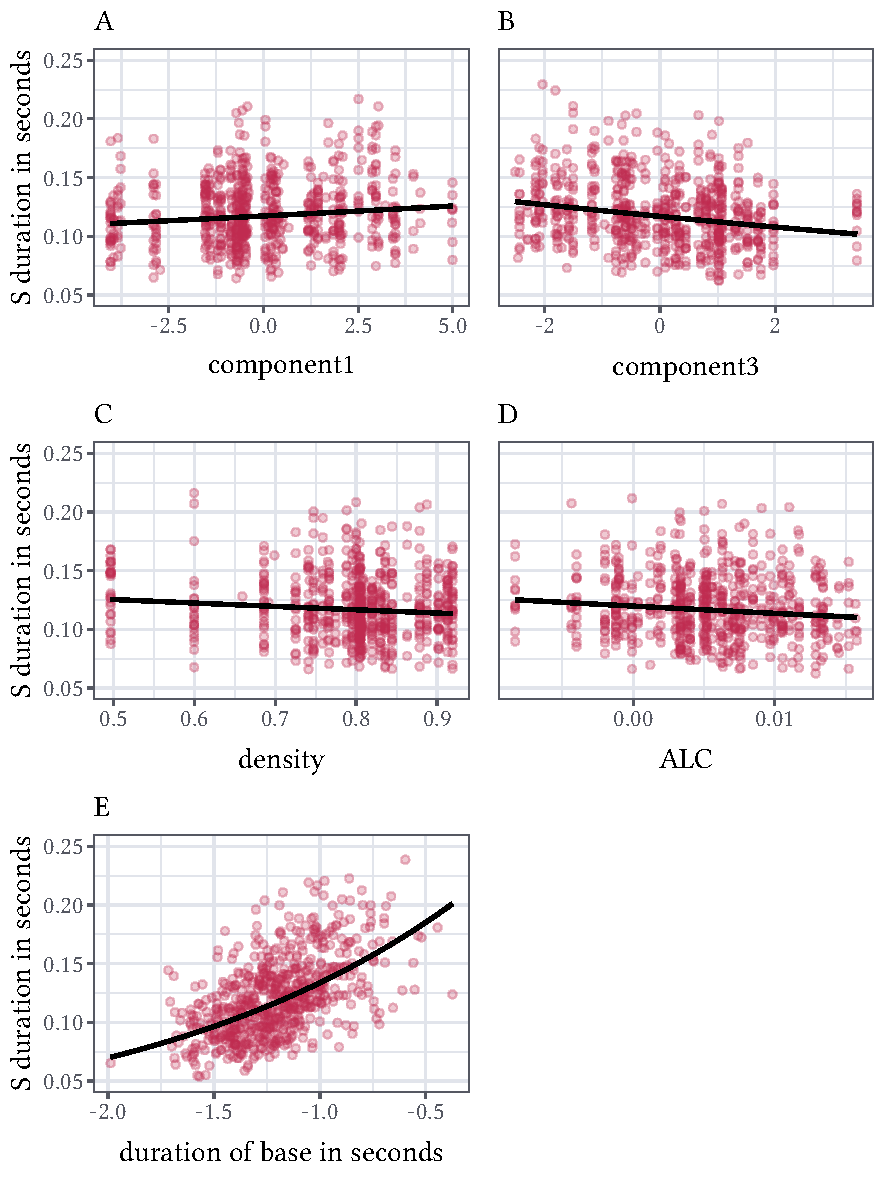
\includegraphics[width=0.9\textwidth]{figures/fig5.1.pdf}
    \caption{Partial effects of the numerical variables \textsc{Component1} (Panel A), \textsc{Component3} (Panel B), \textsc{density} (Panel C), \textsc{ALC} (Panel D), and \textsc{baseDurLog} (back-transformed, Panel E) included in model B, fitted to the log-transformed values of duration of /s/.}
    \label{fig:5_1}
\end{figure}

The partial effects of the categorical variables included in the final model are illustrated in Figure \ref{fig:5_2} Pauses lead to longer /s/ durations (Panel A), which is most likely a case of phrase-final lengthening (e.g. \cite{Cooper1981}). There is also an effect of the following segment type, with /s/ being shorter when followed by a vowel (Panel B). This difference is significant for all consonant types being compared against vowels with the exception of fricatives. However, as there is only a small number of fricative cases in the data, this non-significant difference is potentially not meaningful. Lastly, there is an effect of preceding consonant on /s/ duration (Panel C). /s/ duration is significantly longer if preceded by a voiceless labiodental fricative /f/ or a voiceless velar stop /k/ as compared to cases where /s/ is preceded by a voiceless alveolar stop /t/. All other comparisons are non-significant.

\begin{figure}
    \centering
    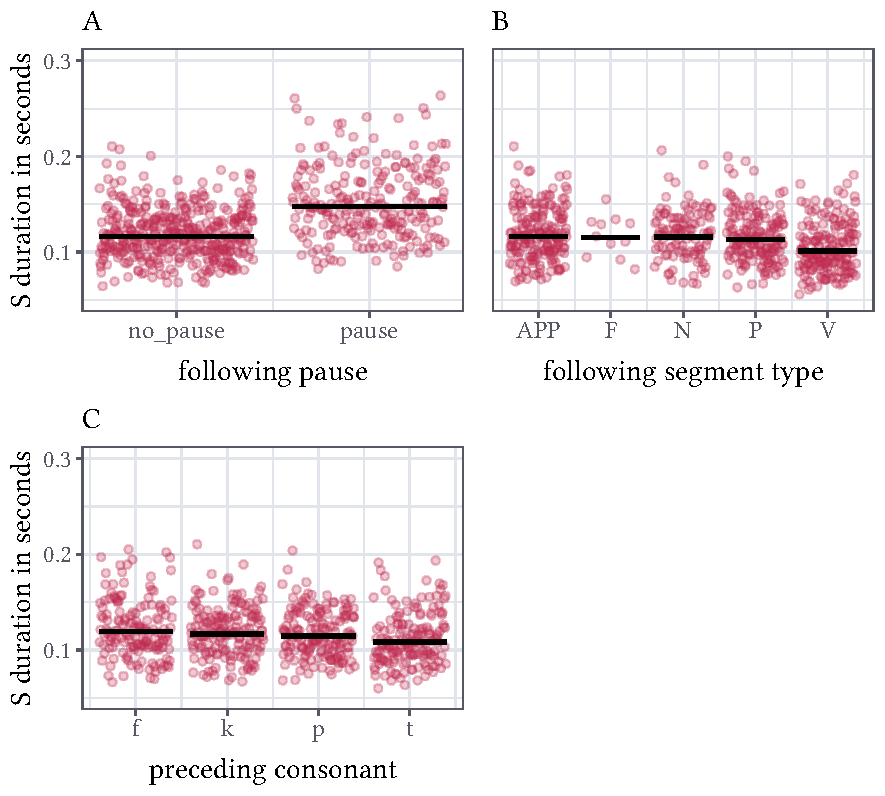
\includegraphics[width=0.9\textwidth]{figures/fig5.2.pdf}
    \caption{Partial effects of the categorical variables \textsc{pauseBin} (Panel A), \textsc{folType} (Panel B), and \textsc{preC} (Panel C) included in model B, fitted to the log-transformed values of duration of /s/.}
    \label{fig:5_2}
\end{figure}

Let us turn to the variables of interest, i.e. those derived from the LDL network. \textsc{Component1} acts as a general measure of phonological certainty. High values of \textsc{Component1} come with high values of \textsc{path\_counts}, \textsc{path\_entropies}, and \textsc{ALDC}, indicating a high level of phonological uncertainty. At the other end of the \textsc{Component1} dimension, high values of \textsc{path\_sum} and \textsc{support} indicate a high level of phonological certainty. Higher uncertainty appears to lead to longer /s/ durations, while higher certainty appears to lead to shorter /s/ durations.

Recall from Section \ref{section05_2_5} that \textsc{Component3} relates to semantic activation diversity and to the presence of the plural suffix. Higher values of \textsc{Component3} indicate a higher level of semantic activation diversity. Higher levels of activation diversity then lead to shorter /s/ durations (see Panel B of Figure \ref{fig:5_1}). High values of \textsc{Component3} are positively correlated with the presence of plural /s/. It appears that the presence of plural makes words semantically more similar to each other as they share this meaning component. Hence, it is to be expected that plural words live in a space of greater semantic activation diversity. \textsc{Component3} is not only a measure of semantic activation diversity, but also indicates that plural pseudowords show a tendency of having a higher degree of semantic activation diversity as compared to monomorphemic pseudowords in general. \textsc{density} and \textsc{ALC} also tap into the semantics of pseudowords. That is, similar to \textsc{Component3}, higher values indicate higher levels of semantic activation diversity. These higher levels then lead to shorter /s/ durations.

\subsection{Model C: LDL measures only}\label{section05_3_3}

The final model of LDL measures only was fitted with effects of the following variables: \textsc{l1norm}, \textsc{ALC}, \textsc{NNC}, log-transformed base duration (\textsc{baseDurLog}), pause (\textsc{pauseBin}), following segmental type (\textsc{folType}), and preceding consonant (\textsc{preC}). The \textsc{speaker} variable was included as random intercept. The \textit{p}-values of the analysis of variance of the final model are given in Table \ref{tab:5.10}.

\begin{table}\fontsize{10}{11}
\caption{\textit{p}-values of fixed effects in model C, fitted to the log-transformed durations of /s/.}
\label{tab:5.10}
\centering
\begin{tabular}{lrrrrrr} 
\lsptoprule
~          & Sum Sq & Mean Sq & NumDF & DenDF  & F.value & Pr(F)  \\ 
\midrule
\textsc{l1norm}     & 0.685  & 0.685   & 1     & 611.07 & 13.473  & 0.000  \\
\textsc{baseDurLog} & 6.047  & 6.047   & 1     & 627.51 & 118.901 & 0.000  \\
\textsc{pauseBin}   & 5.440  & 5.440   & 1     & 632.72 & 106.956 & 0.000  \\
\textsc{folType}    & 2.056  & 0.514   & 4     & 610.10 & 10.105  & 0.000  \\
\textsc{preC}       & 0.761  & 0.254   & 3     & 607.96 & 4.985   & 0.002  \\
\textsc{ALC}        & 0.534  & 0.534   & 1     & 615.51 & 10.504  & 0.001  \\
\textsc{NNC}        & 0.778  & 0.778   & 1     & 619.67 & 15.296  & 0.000  \\
\lspbottomrule
\end{tabular}
\end{table}

With a marginal R\textsuperscript{2} value of $0.41$, the fixed effects of this model explain 41\% of variation within the data. The conditional R\textsuperscript{2} value of the model is $0.61$, that is the complete model accounts for 61\% of variation.

The coefficients of the final model and their \textit{p}-values are given in Table \ref{tab:5.11}. The reference levels for the categorical covariates are: for \textsc{pauseBin} it is \texttt{no\_pause}, for \textsc{folType} it is \texttt{APP}, and for \textsc{preC} it is \texttt{f}.

\begin{table}\fontsize{10}{11}
\caption{Fixed-effect coefficients and \textit{p}-values as computed for model C (mixed-effects model fitted to the log-transformed duration of /s/).}
\label{tab:5.11}
\centering
\begin{tabular}{lrrrrr} 
\lsptoprule
~             & Estimate & SE    & df      & t-value & Pr(\textbar{}t\textbar{})  \\ 
\midrule
(Intercept)   & -2.334   & 0.320 & 625.440 & -7.301  & 0.000                      \\
\textsc{l1norm}        & -0.044   & 0.012 & 611.066 & -3.671  & 0.000                      \\
\textsc{baseDurLog}    & 0.624    & 0.057 & 627.514 & 10.904  & 0.000                      \\
\textsc{pauseBin}pause & 0.233    & 0.022 & 632.719 & 10.342  & 0.000                      \\
\textsc{folType}\texttt{F}      & -0.019   & 0.073 & 613.088 & -0.267  & 0.790                      \\
\textsc{folType}\texttt{N}      & -0.005   & 0.028 & 607.324 & -0.195  & 0.845                      \\
\textsc{folType}\texttt{P}      & -0.023   & 0.024 & 607.817 & -0.950  & 0.343                      \\
\textsc{folType}\texttt{V}      & -0.140   & 0.025 & 611.952 & -5.693  & 0.000                      \\
\textsc{preC}\texttt{k}         & -0.029   & 0.027 & 607.726 & -1.058  & 0.291                      \\
\textsc{preC}\texttt{p}         & -0.053   & 0.027 & 607.478 & -1.950  & 0.052                      \\
\textsc{preC}\texttt{t}         & -0.101   & 0.028 & 608.068 & -3.632  & 0.000                      \\
\textsc{ALC}           & -6.663   & 2.056 & 615.511 & -3.241  & 0.001                      \\
\textsc{NNC}           & 1.221    & 0.312 & 619.671 & 3.911   & 0.000                      \\
\lspbottomrule
\end{tabular}
\end{table}

As for both other final models, the predictor strength of the individual predictors was checked. This procedure resulted in the hierarchy of predictor strength given in \ref{ex:5.3}. That is, the decrease in R\textsuperscript{2} is greatest when removing \textsc{baseDurLog}, followed by \textsc{pauseBin}, and so forth. 

\ex.
\label{ex:5.3}
\textsc{baseDurLog >> pauseBin >> folType >> NNC >> l1norm >> ALC >> preC}

Figure \ref{fig:5_3} displays the effect on /s/ duration of the numerical variables included in the model. Base duration shows an identical effect as compared to model B in Section \ref{section05_3_2}, i.e. longer base durations come with longer /s/ durations. 

\begin{figure}
    \centering
    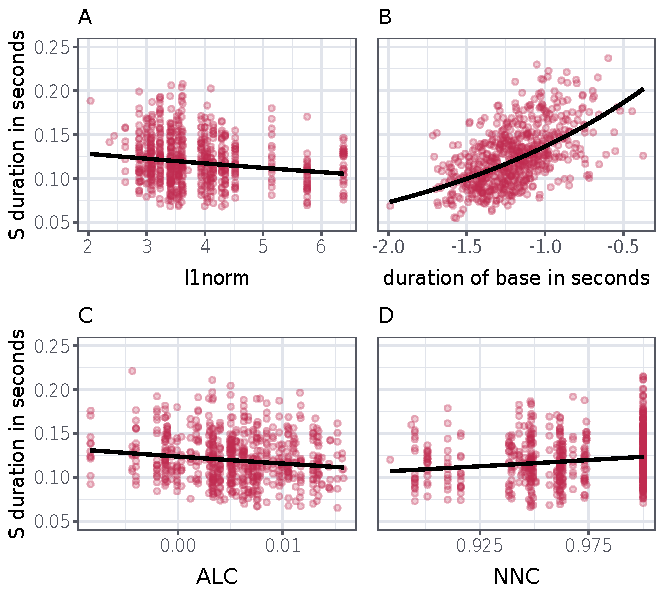
\includegraphics[width=0.9\textwidth]{figures/fig5.3.pdf}
    \caption{Partial effects of the numerical variables \textsc{l1norm} (Panel A), \textsc{baseDurLog} (back-transformed, Panel B), \textsc{ALC} (Panel C), and \textsc{NNC} (Panel D) included in model C, fitted to the log-transformed values of duration of /s/.}
    \label{fig:5_3}
\end{figure}

Figure \ref{fig:5_4} shows the effect on /s/ duration of the categorical variables included in the model. Pauses again come with longer /s/ durations, and /s/ is shorter if followed by a vowel. There is also an effect of the preceding consonant, with /s/ duration being significantly longer if preceded by a voiceless labiodental fricative /f/ or a voiceless velar stop /k/ as compared to cases where /s/ is preceded by a voiceless alveolar stop /t/. These results are generally in line with those by the analysis in the previous section.

\begin{figure}
    \centering
    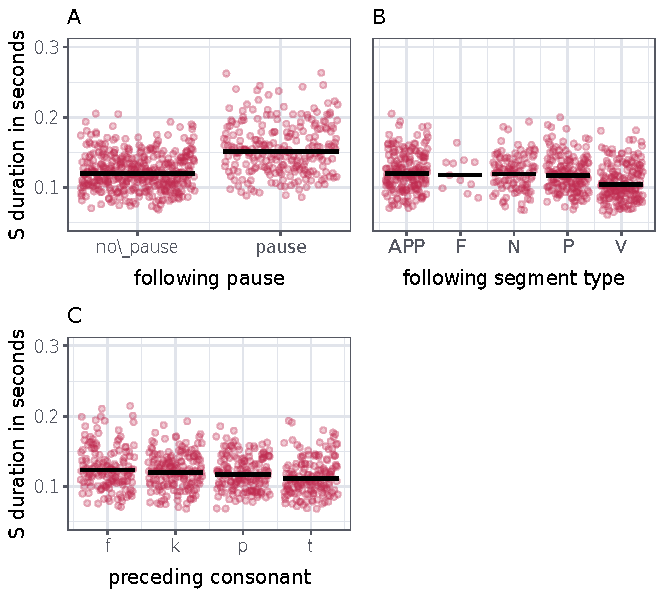
\includegraphics[width=0.9\textwidth]{figures/fig5.4.pdf}
    \caption{Partial effects of the categorical variables \textsc{pauseBin} (Panel A), \textsc{folType} (Panel B), and \textsc{preC} (Panel C) included in model C, fitted to the log-transformed values of duration of /s/.}
    \label{fig:5_4}
\end{figure}

Taking a closer look at the variables of interest, one finds that higher values of \textsc{l1norm} and \textsc{ALC}, i.e. higher semantic activation diversity, lead to shorter /s/ durations. As in model B, higher levels of semantic activation diversity come with shorter /s/ durations. For \textsc{NNC}, it is found that /s/ duration is longer if a pseudoword is semantically similar to a real word.

\section{Discussion}\label{section05_4}

The production study presented in Chapter \ref{chapter04} of this book as well as previous studies (\cite{Zimmermann2016, Plag2017, Seyfarth2017, Tomaschek2019, Plag2020}) reported that there are significant differences in the acoustic duration between different types of word-final /s/ in English. Such durational differences challenge established feed-forward theories of morphology-phonology interaction (e.g. \cite{Chomsky1968, Kiparsky1982}) as well as theories of psycholinguistics (e.g. \cite{Levelt1999, Roelofs2019, Turk2020}). The present study investigated whether measures derived on the basis of a discriminative learning theory are predictive of /s/ durations in pseudowords. In particular, LDL networks that model the production of a word based on its relation to the rest of the lexicon were implemented.

The predictive possibilities of LDL measures were explored by fitting three different models: a) a model based on the traditional predictors as used in previous studies (\cite{Plag2017,,Tomaschek2019}) and most importantly in the production study reported in this book; b) a model with LDL measures and a variable \textsc{typeOfS} specifying the presence or absence of an affix; and c) a model with LDL measures but without a variable specifying the presence or absence of an affix. Both models with LDL measures show that such measures are predictive of /s/ durations. This result is the most important of the present study. While traditional variables such as lexical frequencies, bigram frequencies, transitional probabilities, or neighbourhood densities measure important lexical properties, it is unclear why they would manifest themselves in a particular morphological effect in speech production. In LDL such effects can emerge through the mapping of form and meaning in a clearly defined process of discriminative learning.

All regression models showed a similar hierarchy of predictor strength for the variables included in the models. For the traditional model A, \textsc{typeOfS} is the third-strongest predictor of /s/ duration and for model B this spot is taken by \textsc{Component3}, while there is no comparable variable included in model C. Comparing the variance explained by the fixed effects of the different models, one finds that the traditional model accounts for most variation, i.e. 43\%, while the LDL model including the \textsc{typeOfS} variable accounts for 42\%, and the LDL model without the \textsc{typeOfS} variable accounts for 41\% of variation. Thus, in terms of marginal R\textsuperscript{2} values, all three models are close to each other. To check whether these differences in marginal R\textsuperscript{2} values are of significance, the three models were refitted to the untrimmed data set and then compared with a likelihood-ratio test. The results suggest that there is no significant difference between the traditional model and the LDL model including the \textsc{typeOfS} variable. However, the LDL model without the \textsc{typeOfS} variable shows a significantly worse fit ($p<0.01$). This seems to indicate that the LDL measures do not capture the full amount of the variance that is captured by the variable \textsc{typeOfS}. This means that there is still something about the morphological function that translates into duration and that is not properly modelled by the associative measurements of the learning network. The same problem holds, incidentally, for the traditional model (model A), in which the usual lexical measures (such as lexical frequencies, neighbourhood densities, etc.) and phonetic covariates (such as pauses, speech rate, etc.) are also not able to cover all durational variance. The morphological residue in both types of analysis remains a conundrum that calls for more sophisticated approaches in future research.

The LDL measures included in the final models are either concerned with semantic activation diversity (\textsc{Component3}, \textsc{ALC}, \& \textsc{density} in model B; \textsc{l1norm} \& \textsc{ALC} in model C), semantic similarity (\textsc{NNC} in model C) or with phonological certainty (\textsc{Component1} in model B).

Higher degrees of semantic activation diversity come with shorter /s/ durations. This effect is similar to the one which was reported by \citet{Tucker2019Sims} in a study on stem vowels and \citet{Tomaschek2019} in their NDL study on /s/ duration. A higher degree of activation diversity makes it ``more difficult to discriminate the targeted outcome from its competitors" (\cite[27]{Tomaschek2019}). As for production, a prolongation of the acoustic signal is dysfunctional if the prolongation maintains or increases the discrimination problem instead of contributing to resolving it (\cite{Tomaschek2019}).

In the model without \textsc{typeOfS} as predictor variable, \textsc{NNC} (i.e. a pseudoword’s semantic similarity to its closest semantic real word neighbour) emerges as significant (see model C). Why so? As reported in Section \ref{section05_2_5}, the \textsc{typeOfS} variable and \textsc{NNC} are strongly negatively correlated ($rho = -0.89$). Post-hoc analysis shows that plural /s/ has significantly lower \textsc{NNC} values as compared to non-morphemic /s/ (Wilcoxon test,  $p<0.001$). It therefore appears that \textsc{NNC} takes over the role of differentiating between plural and non-morphemic /s/ in model C.

As for phonological certainty, one finds that higher phonological certainty comes with shorter /s/ durations, while higher phonological uncertainty comes with longer /s/ durations. Shorter durations in contexts of high phonological certainty may be related to effects of frequency, i.e. highly frequent forms are produced with higher certainty and are thus shorter. 

The results of the present study may bring up further questions. First, are the predictive measures found for word-final /s/ duration in pseudowords also predictive for word-final /s/ duration in real words? The NDL implementation of \citet{Tomaschek2019} suggests that they are, but LDL networks still need to be implemented. It would be especially interesting to model those data sets that have yielded seemingly contradictory effects. Second, taking into account that the specification of \textsc{typeOfS} in the modelling process leads to a significantly better model fit, one may ask what the underlying reasons for this significant effect are. This then automatically leads to another question: Is it possible to catch the effect of the \textsc{typeOfS} specification in terms of (new) LDL measures? 

To summarise, this study was the first to investigate durational differences between different types of word-final /s/ (non-morphemic versus plural /s/) in pseudowords by means of an LDL implementation, measures, and resulting statistical analyses. The findings yielded important evidence on the question of how such durational differences come to be, i.e. they can be predicted based on their pseudoword’s relations to the lexicon. It was demonstrated that durational differences emerge from the pseudoword’s resonance with the lexicon by way of differing degrees of semantic activation diversity and phonological uncertainty. These manifestations of the relations to other words in the lexicon in turn are the result of discriminative learning.

%\chapter{Perception of word-final /s/}\label{chapter06}

As introduced in detail in Section \ref{section02_2}, the perception study presented here investigates whether subphonemic durational differences in word-final /s/ are perceived by listeners. Two hypotheses derived from theories and models of speech perception are examined. \textsc{H perc\textsubscript{1}}, the \textit{Abstractionist Hypothesis}, assumes that listeners are not sensitive to subphonemic durational differences. \textsc{H perc\textsubscript{2}}, the \textit{Phonetic Detail Hypothesis}, predicts that subphonemic durational differences are perceptible. Subsequently, listeners are assumed to be sensitive to such differences. The two hypotheses are tested by analysing the results of a same-different task.

\section{Methodology}\label{section06_1}

\subsection{Participants}\label{section06_1_1}

Forty native speakers of New Zealand English took part in the same-different task. One participant had to be excluded right away as they did not respond in any trial. The mean age of the remaining 39 subjects was 23.0 years, ranging from 18 to 39. Six participants identified as multilingual. The experiment took place at the University of Canterbury, Christchurch, New Zealand, from December 2020 to March 2021. 

\subsection{Materials}\label{section06_1_2}

The speech materials consisted of pseudowords as well as of real words and real word filler items. As the aim of the present experiment was to study the perception of word-final /s/, only those pseudowords with word-final /s/ were used. The 24 pseudowords used as stimuli were introduced in Section \ref{section03_1_2}. For reasons of convenience, Table \ref{tab:6.1} lists these pseudowords once more.

\begin{table}\fontsize{10}{11}
\caption{Orthographic (\textit{orth.}) and phonological (\textit{phon.}) representations of the pseudowords used in the same-different task.}
\label{tab:6.1}
\centering
\begin{tabular}{lllllll} 
\lsptoprule
~              & /glɪ/          & /prʌ/          & /pli:/          & /clu:/          & /blaʊ/          & /gleɪ/           \\ 
\midrule
\textit{orth.} & \textit{glips} & \textit{prups} & \textit{pleeps} & \textit{cloops} & \textit{bloups} & \textit{glaips}  \\
\textit{phon.} & /glɪps/        & /prʌps/        & /pli:ps/        & /klu:ps/        & /blaʊps/        & /gleɪps/         \\ 
\midrule
\textit{orth.} & \textit{glits} & \textit{pruts} & \textit{pleets} & \textit{cloots} & \textit{blouts} & \textit{glaits}  \\
\textit{phon.} & /glɪts/        & /prʌts/        & /pli:ts/        & /klu:ts/        & /blaʊts/        & /gleɪts/         \\ 
\midrule
\textit{orth.} & \textit{gliks} & \textit{pruks} & \textit{pleeks} & \textit{clooks} & \textit{blouks} & \textit{glaiks}  \\
\textit{phon.} & /glɪks/        & /prʌks/        & /pli:ks/        & /klu:ks/        & /blaʊks/        & /gleɪks/         \\ 
\midrule
\textit{orth.} & \textit{glifs} & \textit{prufs} & \textit{pleefs} & \textit{cloofs} & \textit{bloufs} & \textit{glaifs}  \\
\textit{phon.} & /glɪfs/        & /prʌfs/        & /pli:fs/        & /klu:fs/        & /blaʊfs/        & /gleɪfs/         \\
\lspbottomrule
\end{tabular}
\end{table}

The set of twelve real words used in this experiment was also introduced in Section \ref{section03_1_2}. Recall that words were taken from the British National Corpus (\cite{Davies2004}), following a number of criteria. That is, words had to have a word-final /s/ as part of a voiceless stop plus sibilant coda; they had to be either singular or plural nouns with one syllable; and the number of short monophthong, long monophthong, and diphthong nuclei had to be equally distributed across words for both singular and plural nouns. For singular /s/, it was not possible to fully meet the final criterion as there was only one word with a long monophthong nucleus. Another monomorphemic word with a short monophthong was used instead. The set of real words is given in Table \ref{tab:6.2}.

\begin{table}\fontsize{10}{11}
\caption{Real words used in the same-different task.}
\label{tab:6.2}
\centering
\begin{tabular}{llll} 
\lsptoprule
\multicolumn{2}{c}{Non-morphemic /s/} & \multicolumn{2}{c}{Plural suffix /s/}  \\ 
\midrule
Item            & Vowel quality       & Item            & Vowel quality        \\
\midrule
\textit{mix}    & short               & \textit{books}  & short                \\
\textit{box}    & short               & \textit{steps}  & short                \\
\textit{tax}    & short               & \textit{rights} & diphthong            \\
\textit{coax}   & diphthong           & \textit{points} & diphthong            \\
\textit{hoax}   & diphthong           & \textit{groups} & long                 \\
\textit{corpse} & long                & \textit{parts}  & long                 \\
\lspbottomrule
\end{tabular}
\end{table}

Additionally, twelve filler items were employed. All filler items were singular nouns consisting of a single syllable with either a short monophthong, a long monophthong, or a diphthong as nucleus. The nucleus type followed the same distribution as for the items described above, i.e. one third of filler items per type of nucleus. Half of the filler items ended in /f/, while the other half ended in /θ/. See Table \ref{tab:6.3} for all filler items.

\begin{table}\fontsize{10}{11}
\caption{Filler items used in the same-different task.}
\label{tab:6.3}
\centering
\begin{tabular}{llll} 
\lsptoprule
\multicolumn{2}{c}{Non-morphemic /s/} & \multicolumn{2}{c}{Plural suffix /s/}  \\ 
\midrule
Item            & Vowel quality       & Item            & Vowel quality        \\
\midrule
\textit{riff}    & short               & \textit{death}  & short                \\
\textit{muff}    & short               & \textit{myth}  & short                \\
\textit{wife}    & diphthong               & \textit{faith} & diphthong            \\
\textit{safe}   & diphthong           & \textit{growth} & diphthong            \\
\textit{grief}   & diphthong           & \textit{booth} & long                 \\
\textit{hoof} & long                & \textit{path}  & long                 \\
\lspbottomrule
\end{tabular}
\end{table}

The recording of the speech materials took place at a soundproof booth of the Department of Linguistics at the University of Tübingen. For this, reading lists were created. On these lists, items were embedded within the sentence ``He said \textit{item} to me.". A trained native speaker of New Zealand English read the entire reading list aloud for practice before recording the list three times. The recordings were sampled at 44.1 kHz, 16 bit.

For each item the best of the three recordings was chosen by manual inspection. First, all recordings were analysed using Praat following the segmentation conventions laid out in Section \ref{section04_1_4}. Recordings with production errors, e.g. laughter, stutter or vocal fry, or segmentation difficulties were dismissed. Second, the remaining segmented target and filler items were spliced from their surrounding contexts, resulting in audio files only containing the words of interest. Third, the duration of the items and filler items was measured using a Praat script (\cite{deJong2008}) and then analysed in R. The result of this analysis is given as the mean durations presented in Table \ref{tab:6.4}. Lastly, for each item the version closest to the mean duration of its nucleus type was chosen for further use in the experiment to keep durational differences between items to a minimum.

\begin{table}\fontsize{10}{11}
\caption{Mean durations of items and filler items across recordings in seconds.}
\label{tab:6.4}
\centering
\begin{tabular}{llccc} 
\lsptoprule
Item type   & ~                                                                   & Short vowel                                           & Long vowel                                            & Diphthong                                              \\ 
\midrule
real words  & \begin{tabular}[c]{@{}l@{}}\textit{mean} \\\textit{sd}\end{tabular} & \begin{tabular}[c]{@{}l@{}}0.576 \\0.109\end{tabular} & \begin{tabular}[c]{@{}l@{}}0.613 \\0.102\end{tabular} & \begin{tabular}[c]{@{}l@{}}0.572 \\0.062\end{tabular}  \\ 
\midrule
pseudowords & \begin{tabular}[c]{@{}l@{}}\textit{mean} \\\textit{sd}\end{tabular} & \begin{tabular}[c]{@{}l@{}}0.521 \\0.060\end{tabular} & \begin{tabular}[c]{@{}l@{}}0.551 \\0.042\end{tabular} & \begin{tabular}[c]{@{}l@{}}0.550 \\0.046\end{tabular}  \\ 
\midrule
filler      & \begin{tabular}[c]{@{}l@{}}\textit{mean} \\\textit{sd}\end{tabular} & \begin{tabular}[c]{@{}l@{}}0.455 \\0.052\end{tabular} & \begin{tabular}[c]{@{}l@{}}0.490 \\0.067\end{tabular} & \begin{tabular}[c]{@{}l@{}}0.549 \\0.071\end{tabular}  \\
\lspbottomrule
\end{tabular}
\end{table}

In a next step, the final /s/ duration of all items was manipulated in such a way that it corresponded to the mean /s/ duration for non-morphemic and plural /s/ found in the reference study by \citet{Plag2017}. For example, in the case of \textit{mix} the duration of the final /s/ was changed to 318 ms, while in the case of \textit{books} the duration of the final /s/ was changed to 283 ms. This was done for all items, i.e. real words and pseudowords. 

Pseudowords were treated as both singular and plural nouns. That is, pseudowords were equally distributed across four groups as follows. First, each group consisted of at least one pseudoword ending in /ps/, /ts/, /ks/, and /fs/. Second, groups A and B had two additional pseudowords ending in /ps/ and /ts/, respectively, while groups C and D had two additional pseudowords ending in /ks/ and /fs/, respectively. See Table \ref{tab:6.5} for the distribution of pseudowords across groups. 

\begin{table}\fontsize{10}{11}
\caption{Pseudoword distribution across the groups A-D used in the same-different task.}
\label{tab:6.5}
\centering
\begin{tabular}{lcccc} 
\lsptoprule
~     & Group A & Group B & Group C & Group D  \\ 
\midrule
gli-  & ps      & ts      & ks      & fs       \\
plee- & ts      & ps      & fs      & ks       \\
cloo- & ks      & ts      & ps      & fs       \\
pru-  & fs      & ks      & ts      & ps       \\
blou- & ps      & fs      & ks      & ts       \\
glai- & ts      & ps      & fs      & ks       \\
\lspbottomrule
\end{tabular}
\end{table}

The pseudowords in groups A and C were treated as singular nouns with a non-morphemic word-final /s/, while the pseudowords in groups B and D were treated as plural nouns with a plural word-final /s/. Their /s/ durations were changed accordingly. This way of handling type of /s/ across pseudowords was chosen to keep priming effects across pseudowords to a minimum, i.e. no participant was to encounter pseudowords with both singular and plural /s/ durations. 

Then, four altered versions of each modified item were created. Each non-morphemic /s/ item was edited in such a way that 10 ms, 20 ms, 35 ms, or 75 ms were subtracted from the word-final /s/ duration, making it gradually more similar to plural word-final /s/ in terms of its duration. For plural /s/ items, 10 ms, 20 ms, 35 ms, or 75 ms were added to the word-final /s/ duration, making it gradually more similar to non-morphemic word-final /s/ in terms of its duration. This resulted in five different /s/ durations per recorded item. See Table \ref{tab:6.6} for all final /s/ durations across non-morphemic and plural /s/ items. Depending on the pertinent item, the duration of the word-final /s/ took up more than half of the total word duration (cf. Table \ref{tab:6.4} and Table \ref{tab:6.6}) and was notably longer than the original non-edited /s/ which showed a mean duration of 174 ms. Nonetheless, all items sounded natural. In total, five versions for each of the 12 real word items and for each of the 24 pseudoword items were created, resulting in 180 items. Each participant was to listen to 90 of them, i.e. (12 real words + 6 pseudowords) × 5 versions.

\begin{table}\fontsize{10}{11}
\caption{Durations in milliseconds for non-morphemic and plural /s/ for real word and pseudoword items.}
\label{tab:6.6}
\centering
\begin{tabular}{lccccc} 
\lsptoprule
~             & Mean & ± 10 ms & ± 20 ms & ± 35 ms & ± 75 ms  \\ 
\midrule
non-morphemic & 318  & 308     & 298     & 283     & 243      \\
plural        & 283  & 293     & 303     & 318     & 358      \\
\lspbottomrule
\end{tabular}
\end{table}

A similar approach was used for the manipulation of filler items. Their final fricative duration was altered as well. For this, the mean duration of word-final /f/ and /θ/ was measured after extracting the recorded filler items from their contexts. It was found that the mean duration of word-final /f/ was 244 ms, while the mean duration of /θ/ was 217 ms. It was therefore decided that the duration of /f/ was treated similarly to that of non-morphemic /s/, i.e. it was shortened, while the duration of /θ/ was treated similarly to that of plural /s/, i.e. it was lengthened. The different durations for both /f/ and /θ/ are given in Table \ref{tab:6.7}.

\begin{table}\fontsize{10}{11}
\caption{Durations in milliseconds for /f/ and /θ/ for filler items.}
\label{tab:6.7}
\centering
\begin{tabular}{lccccc} 
\lsptoprule
~             & Mean & ± 10 ms & ± 20 ms & ± 35 ms & ± 75 ms  \\ 
\midrule
/f/ filler items & 244  & 234     & 224     & 209     & 169      \\
/θ/ filler items & 217  & 227     & 237     & 252     & 292      \\
\lspbottomrule
\end{tabular}
\end{table}

\subsection{Procedure}\label{section06_1_3}

The same-different task was conducted in OpenSesame (\cite{Mathot2012}). First, participants were introduced to the same-different task. They were told that during the following experiment, they were to hear two recordings of the same word at a time and that they had to decide whether these two recordings were identical or different. It was explained that they should decide as quickly as possible and answer by pressing either the \textit{same} or \textit{different} key on the keyboard. The key assigned to \textit{same} was ``A", the key assigned to \textit{different} was ``K". The ``A" key was pressed using the left index finger, the ``K" key was pressed using the right index finger. Both options were given on screen during the entire experiment as illustrated by Figure \ref{fig:6_1}. The participants were also told that if they did not decide on either option within a certain amount of time, the next trial would start automatically. Each participant started with ten practice trials, which consisted of six pseudoword items for familiarisation and four filler items.

\begin{figure}
    \centering
    \includegraphics[width=0.7\textwidth]{figures/fig6.1.png}
    \caption{Option display during the perception experiment.}
    \label{fig:6_1}
\end{figure}

Each trial was preceded by a fixation cross and a stretch of silence of 450 ms. Then, both recordings played, with reaction time measurement starting at the onset of the second recording. The word-final /s/ of both recordings was either similar or different in duration, following one of the possible combinations given in Table \ref{tab:6.8}, resulting in a trial number of 270, i.e. (12 real word items + 6 pseudoword items + 12 filler items) × 9 combinations. The experiment was split into four main parts to allow for short pauses. Each part consisted of either 67 or 68 trials 
(67 × 2 + 68 × 2 = 270). Within each of the four parts, target and filler items were distributed evenly but pseudorandomised, i.e. it was prevented that two trials in a row neither contained the same target or filler item nor the same combination of /s/ durations.

\begin{table}\fontsize{10}{11}
\caption{Combinations of /s/ durations used in the same-different task. \textit{mean} is the mean duration found in \citet{Plag2017} for non-morphemic and plural /s/. ± represents a subtraction for non-morphemic /s/ items and an addition for plural /s/ items.}
\label{tab:6.8}
\centering
\begin{tabular}{llll}
\lsptoprule
Same/different & /s/ durations of items                                                     & Same/different & /s/ durations of items                                             \\
\midrule
same           & mean vs. mean                                                            & different      & \begin{tabular}[c]{@{}l@{}}mean vs.\\ mean ± 10 ms\end{tabular}  \\
same           & \begin{tabular}[c]{@{}l@{}}mean ± 10 ms vs. \\ mean ± 10 ms\end{tabular} & different      & \begin{tabular}[c]{@{}l@{}}mean vs.\\ mean ± 20 ms\end{tabular}  \\
same           & \begin{tabular}[c]{@{}l@{}}mean ± 20 ms vs. \\ mean ± 20 ms\end{tabular} & different      & \begin{tabular}[c]{@{}l@{}}mean vs.\\ mean ± 35 ms\end{tabular}  \\
same           & \begin{tabular}[c]{@{}l@{}}mean ± 35 ms vs. \\ mean ± 35 ms\end{tabular} & different      & \begin{tabular}[c]{@{}l@{}}mean vs.\\ mean ± 75 ms\end{tabular}  \\
same           & \begin{tabular}[c]{@{}l@{}}mean ± 75 ms vs. \\ mean ± 75 ms\end{tabular} & ~              & ~          \\
\lspbottomrule
\end{tabular}
\end{table}

Participants were given a 2,000 ms window to react, starting after the offset of the second recording. After that a time-out was recorded. The next trial automatically started 2,500 ms after the offset of the second recording if no reaction was recorded.

\section{Analysis}\label{section06_2}

Data of same-different tasks are often analysed in terms of their error-rates (e.g. \cite{Belke2002, Norris2008errorrates, Lupker2018}). For example, if a certain condition A shows a significantly higher error rate as compared to another condition B, it is concluded that perception of condition A is significantly worse. Figure \ref{fig:6_2} shows the overall error rates of the present same-different task results.

\begin{figure}
    \centering
    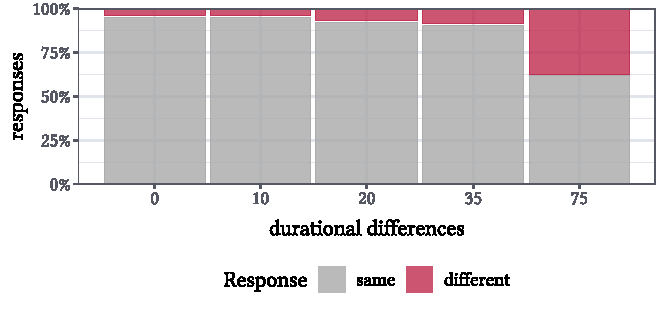
\includegraphics[]{figures/fig6.2.pdf}
    \caption{Overall error rates for the same-different task for all durational differences and across all subjects. For a durational difference of 0 ms the error rate is represented by the part of the bar corresponding to \texttt{different}, while for all other durational differences the error rate is the given part of the pertinent bars corresponding to \texttt{same}.}
    \label{fig:6_2}
\end{figure}

For a durational difference of 0 ms, the error rate is rather low with about 4\%. For the 10 ms difference, the error rate is 96\%; for the 20 ms difference, the error rate is 93\%; for the 35 ms difference, the error rate is 91\%; and for the 75 ms difference, the error rate is 62\%. However, the overall results do not take into account inter-subject differences. It may very well be the case that some participants are more sensitive to durational differences or that some participants simply were more motivated to deliver a good performance. Figure \ref{fig:6_3} shows the overall results for all participants. 

One can clearly see that some participants outperform others. For example, participant \textit{s035} already improves their error rate at a difference of 20 ms, while participant \textit{s030} shows virtually no correct responses for durational differences between 10 ms and 35 ms, and only some for 75 ms.

\begin{figure}
    \centering
    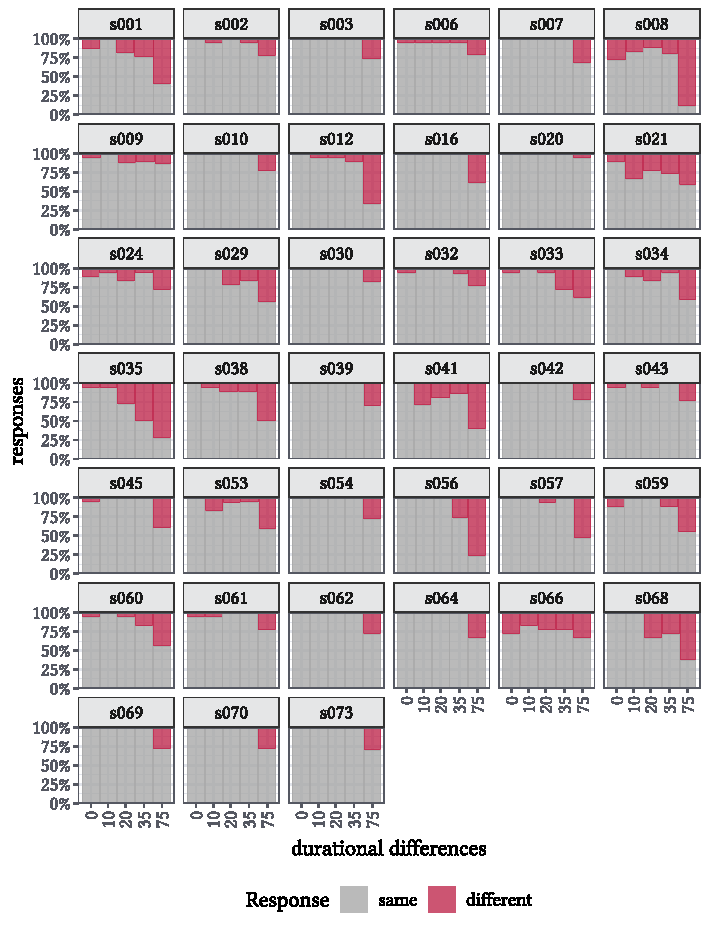
\includegraphics[]{figures/fig6.3.pdf}
    \caption{Error rates per subject for the same-different task for all durational differences. For a durational difference of 0 ms the error rate is represented by the part of the bar corresponding to \texttt{different}, while for all other durational differences the error rate is the given part of the pertinent bars corresponding to \texttt{same}.}
    \label{fig:6_3}
\end{figure}

One possible way to proceed from these descriptive findings is to fit a statistical model to the data. However, as has become visible, there are clear differences between subjects, which points towards another issue: Individuals may have different levels of conservativity. That is, a more conservative participant will less often respond with \textit{different}, while a less conservative participant will more often respond with \textit{different}, irrespective of the stimuli they hear. This intra-subject bias is neglected if one was to use the raw data, as was done in this section thus far.

A common way to factor in this participant bias is to make use of Signal Detection Theory (e.g. \cite{Macmillan1993,Macmillan2005}) and its measures. Signal Detection Theory can be applied in the analysis of any experiment in which two possible stimulus types are to be discriminated, i.e. in which error rates are the dependent variable of interest. The different measures of Signal Detection Theory have been used to analyse, among other things, recognition memory, lie detection, personnel selection, jury decision-making, medical diagnosis, industrial inspection, information retrieval, and congenital amusia (e.g. \cite{Stanislaw1999, Pfeifer2018}). Signal Detection Theory makes use of \textit{all four cells} of discriminative results as illustrated in the toy example in Table \ref{tab:6.9}.

\begin{table}\fontsize{10}{11}
\caption{Types of results for a discriminative task as described by type of stimulus and type of response. Values illustrate a toy example.}
\label{tab:6.9}
\centering
\begin{tabular}{lcccc}
\lsptoprule
\textbf{~}          & \multicolumn{2}{c}{response: different} & \multicolumn{2}{c}{response: same}  \\
\midrule
stimulus: different & \textsc{hit}         & 20                        & \textsc{miss}              & 5               \\
stimulus: same      & \textsc{false alarm} & 10                        & \textsc{correct rejection} & 15              \\
\lspbottomrule
\end{tabular}
\end{table}

To calculate the most commonly used Signal Detection Theory measure, a bias-free measure of subject sensitivity called $d'$, one must first calculate the hit rate $H$

\begin{equation}
\label{eq:H}
    H=\frac{HIT}{HIT+MISS}
\end{equation}

\noindent and the false alarm rate $F$

\begin{equation}
\label{eq:F}
    F=\frac{FALSE\ ALARM}{FALSE\ ALARM + CORRECT\ REJECTION}\ .
\end{equation}

Then, $d'$ can be computed as

\begin{equation}
\label{eq:dprime}
    d'=z(H)-z(F)
\end{equation}

\noindent where $z(.)$ is the Z-transform of either variable. However, $d'$ can only be meaningfully used if two assumptions regarding the decision variable are met (\cite{Stanislaw1999}). First, the signal and noise distributions are both normal. Second, the signal and noise distributions have the same standard deviation. In the present case, noise is equivalent to trials with two identical stimuli. If one of the assumptions is violated, $d'$ will vary with the response bias (\cite{Stanislaw1999}). Thus, it was decided to use an alternative measure, $A'$, instead. $A'$ is a nonparametric variant of $d'$ (\cite{Pollack1964}) and its values range between $0$ and $1$, where higher values indicate higher sensitivity, and $1$ indicates perfect performance. $H$ and $F$, as introduced above, are also used to calculate $A'$:

\begin{equation}
\label{eq:aprime}
    A'=0.5+\left [ sign(H-F)\frac{(H-F)^2+|H-F|}{4max(H,F)-4HF}\right ],
\end{equation}

\noindent where the term $sign(H-F)$ is $+1$ if $H-F>0$, $0$ if $H=F$, and $-1$ otherwise. $max⁡(H,F$) equals either $H$ or $F$, whichever is greater (\cite{Stanislaw1999}). For the above toy example given in Table \ref{tab:6.9}, $A'$ then is

\begin{equation}
\label{eq:aprimeex}
    A'=0.5+\left [ \frac{(0.8-0.4)^2+|0.8-0.4|}{4*0.8-4*0.8*0.4}\right ],
\end{equation}

\noindent that is, $A'$ has a value of about $0.79$. Thus, in the example, sensitivity is quite high.

In the following sections, I will first introduce the covariates used in the analysis of the same-different task data. Then, I will present the analysis of the data, including the calculation of $A'$ values from the raw data, and the statistical modelling of $A'$ as dependent variable.

\subsection{Covariates}\label{section06_2_1}

The set of covariates used in the analysis of the subject sensitivity data calculated from the same-different task results is more restricted than other sets of covariates in this book. As $A'$ values are calculated across all trials of a subject, item specific variables such as \textsc{typeOfS} (\texttt{non-morphemic} versus \texttt{plural}) and \textsc{typeOfWord} (\texttt{real word} versus \texttt{pseudoword}) cannot be used as covariates. However, analysing the raw data with chi-square tests strongly suggests that no significant difference for these variables were found ($p>0.05$ for all comparisons; see the supplementary material given in Chapter \ref{Supplementary Material}). As sensitivity may very well vary between subjects, an additional covariate on how regularly subjects play musical instruments was introduced. In the following, covariates used in previous studies of this book are described first. For these, definitions are briefly repeated for convenience and adapted to perception where necessary. Then, the newly introduced covariate is given. Finally, the covariate used as random effect is listed.

\textsc{age}. Subjects’ \textsc{age} was included as it may show an influence on hearing capabilities, with older subjects often experiencing a loss of hearing (e.g. \cite{Lee2013}).

\textsc{monoMultilingual}. To account for potential influences of other L1s besides English, the binary covariate \textsc{monoMultilingual} was introduced. 

\textsc{musicalInstrument}. It has been shown that advanced players of musical instruments show an increased performance of phonological perception and of detecting durational differences in speech (e.g. \cite{Anvari2002,Milovanov2009}). Thus, information on how regularly each subject plays a musical instrument was collected.

\textsc{subject}. \textsc{subject} ID was included to account for inter-speaker differences in perception.

Closer inspection of the newly introduced covariate, \textsc{musicalInstrument}, revealed that there was an uneven distribution of subjects across levels. That is, only 5\% (n = 8) of trials had \textsc{very often} as value for \textsc{musicalInstrument}, while 41\% (n = 64) had \textsc{never} as value. This skewed distribution is maintained by the levels in between, with 8\% \textsc{often} (n = 12), 20\% \textsc{sometimes} (n = 32), and 26\% \textsc{rarely} (n = 40). Due to the skewed distribution and the therefore small amount of data points for some levels, it was decided to drop \textsc{musicalInstrument} as a covariate. If there was an effect of \textsc{musicalInstrument} nonetheless, this should then be indirectly considered as part of the \textsc{subject} random effect.

\subsection{Overview of the data}\label{section06_2_2}

An overview of all variables used in the analysis of subject sensitivity and their distribution is given in Table \ref{tab:6.10}.

\begin{table}\fontsize{10}{11}
\caption{Summary of the dependent variable and the numerical and categorical predictors in the final data set.}
\label{tab:6.10}
\centering
\begin{tabular}{lllll} 
\lsptoprule
Dependent variable     & \multicolumn{1}{r}{Mean}        & \multicolumn{1}{r}{St. Dev.}                 & \multicolumn{1}{r}{Min}         & \multicolumn{1}{r}{Max}                       \\ 
\midrule
\textsc{aprime}                 & \multicolumn{1}{r}{0.323}       & \multicolumn{1}{r}{0.131}                    & \multicolumn{1}{r}{0.226}       & \multicolumn{1}{r}{0.904}                     \\ 
\midrule
Numerical predictors   & \multicolumn{1}{r}{Mean}        & \multicolumn{1}{r}{St. Dev.}                 & \multicolumn{1}{r}{Min}         & \multicolumn{1}{r}{Max}                       \\ 
\midrule
\textsc{age}                    & \multicolumn{1}{r}{23.000}      & \multicolumn{1}{r}{5.235}                    & \multicolumn{1}{r}{18.000}      & \multicolumn{1}{r}{39.000}                    \\ 
\midrule
Categorical predictors & Levels      & ~                        & ~           & ~                         \\ 
\midrule
\textsc{monoMultilingual}       & \multicolumn{2}{l}{\texttt{monolingual}:
  128} & \multicolumn{2}{l}{\texttt{multilingual}:
  28}  \\
\textsc{subject}                & 39          & ~                        & ~           & ~                         \\ 
\midrule
Explanatory variable   & Levels      & ~                        & ~           & ~                         \\ 
\midrule
\textsc{durDif}                 & \texttt{10 ms}:
  39 & \texttt{20 ms}:
  39              & \texttt{35 ms}:
  39 & \texttt{75 ms}:
  39               \\
\lspbottomrule
\end{tabular}
\end{table}

\subsection{Modelling subject sensitivity}\label{section06_2_3}

Using the formula for calculating $A'$ as given in Equation \ref{eq:aprime} and as implemented by the \texttt{psycho} package for R (\cite{Makowski2018}), $A'$ values for all subjects were computed. That is, for each subject, the results for the four durational differences 10 ms, 20 ms, 35 ms, and 75 ms were used to calculate an $A'$ value. This resulted in four $A'$ values per participant. The four durational differences are the predictor of interest in the regression modelling: \textsc{durDif}.

These $A'$ values then entered a regression analysis as dependent variable. As $A'$ assumes values in the standard unit interval $(0,1)$, regression models such as LMERs or gaussian GAMMs are not sufficient, because such models do not take into account the interval constraint of the dependent variable. As a workaround, one could transform the $A'$ values using, for example, a logit-transformation. However, this comes with several drawbacks (cf. \cite{Cribari2010}). It was thus decided to use beta regression as briefly introduced in Section \ref{section03_2_2} as the statistical tool of choice instead. Beta regression models assume that the dependent variable follows a beta distribution, i.e. that it assumes values in the open interval of $(0,1)$. Commonly, beta regression in R is done using the \texttt{betareg} package (\cite{Cribari2010}). However, the \texttt{betareg} implementation does not allow for random effects in its model specification. As it was plausible to assume inter-subject differences in the given context, the \texttt{mgcv} package (\cite{Wood2017}) and its GAMM implementation were made use of instead. While the default for GAMMs is to assume a dependent variable of gaussian distribution, GAMMs can also be specified for dependent variables following a beta distribution. This is what I call BGAMMs (see Section \ref{section03_2_2}).

A BGAMM was fitted with $A'$ as dependent variable. The predictor of interest, \textsc{durDif}, and the covariate \textsc{monoMulitlingual} were included as parametric effects. \textsc{age} was included as smooth term and \textsc{subject} was specified as random smooth term. Following the procedure introduced in Section \ref{section03_2_2}, the model was checked for issues of concurvity and of too few basis functions; no issues were found. The final data set as well as the analysis and results discussed in the following sections can be found in the supplementary material given in Chapter \ref{Supplementary Material}.

\section{Results}\label{section06_3}

A significant effect of \textsc{durDif} was found. Neither the effect of \textsc{monoMulitlingual} nor the effect of \textsc{age} reached significance. As anticipated, the random smooth of \textsc{subject} reached significance. This was to be expected due to the vast differences between subjects already found in the raw data. The results of the BGAMM fitted to the $A'$ values are given in Table \ref{tab:6.11}. For the parametric terms, I provide the β estimates and the corresponding standard errors (SE), \textit{z}-values, and \textit{p}-values. For the smooth terms, the estimated degrees of freedom, the reference degrees of freedom, the χ\textsuperscript{2} values, and the \textit{p}-values are given.

\begin{table}\fontsize{10}{11}
\caption{Summary of the BGAMM fitted to the $A'$ values with \textsc{durDif} and \textsc{monoMultilingual} as parametric predictors, \textsc{age} as smooth term, and \textsc{subject} as random smooth term.}
\label{tab:6.11}
\centering
\begin{tabular}{lrrrr} 
\lsptoprule
Parametric Terms    & Estimate & SE     & z value & Pr(\textbar{}z\textbar{})  \\ 
\midrule
(Intercept)         & -1.008   & 0.079  & -12.818 & 0.000                      \\
\textsc{durDif20}            & 0.125    & 0.079  & 1.578   & 0.114                      \\
\textsc{durDif35}            & 0.206    & 0.077  & 2.676   & 0.007                      \\
\textsc{durDif75}            & 0.993    & 0.069  & 14.358  & 0.000                      \\
\textsc{monoMultilingual}    & -0.089   & 0.137  & -0.648  & 0.517                      \\ 
\midrule
Smooth Terms        & edf      & Ref.df & Chi.sq  & \textit{p}-value           \\ 
\midrule
\textsc{age}                 & 1.000    & 1.000  & 0.001   & 0.982                      \\ 
\midrule
Random Smooth Terms & edf      & Ref.df & Chi.sq  & \textit{p}-value           \\ 
\midrule
\textsc{subject}             & 28.400   & 36.000 & 144.904 & 0.000                      \\
\lspbottomrule
\end{tabular}
\end{table}

Figure \ref{fig:6_4} shows the partial effect of \textsc{durDif}. Participants show overall little sensitivity towards durational differences of 10 ms and 20 ms. For 35 ms a rather small but nonetheless significant increase in sensitivity is found as compared to the 10 ms difference. A clear increase in sensitivity is found for the durational difference of 75 ms as compared to the other differences. Thus, perceptibility of the 10 ms and 20 ms differences is rather low; the perceptibility of the 35 ms is significantly higher; and the perceptibility of the 75 ms difference is highest.

\begin{figure}
    \centering
    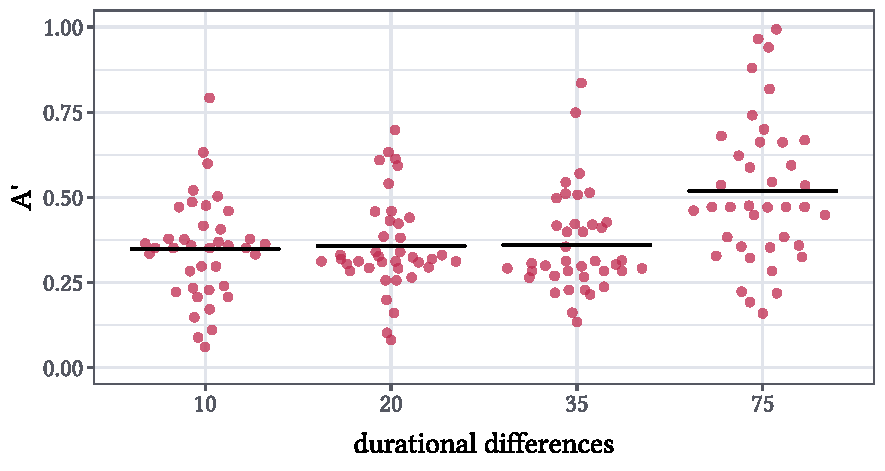
\includegraphics[width=0.9\textwidth]{figures/fig6.4.pdf}
    \caption{Partial effect of \textsc{durDif} as found by the BGAMM. The horizontal lines indicate the estimated $A'$ mean for each durational difference; the points illustrate subject-specific estimates.}
    \label{fig:6_4}
\end{figure}

The overall significant differences in sensitivity are given in Table \ref{tab:6.12}. Participants are significantly more sensitive towards the 75 ms difference as compared to all other durational differences. 

\begin{table}\fontsize{10}{11}
\caption{Significant contrasts found for the different /s/ durations contrasted in the same-different task. Significance codes: *** $p < 0.001$, ** $p < 0.01$, * $p < 0.05$.}
\label{tab:6.12}
\centering
\begin{tabular}{lrrrr} 
\lsptoprule
\textbf{~} & 10~ms & 20~ms & 35~ms & 75~ms  \\ 
\midrule
10~ms      & n.a.  & ~     & **    & ***    \\
20~ms      & ~     & n.a.  & ~     & ***    \\
35~ms      & ~     & ~     & n.a.  & ***    \\
75~ms      & ~     & ~     & ~     & n.a.   \\
\lspbottomrule
\end{tabular}
\end{table}

As shown by the subject-specific $A'$ estimates indicated by points in Figure \ref{fig:6_4}, however, inter-subject differences remain high. Especially the biggest durational difference, 75 ms, shows a discernible amount of variation. The raw by-subject $A'$ values as illustrated in Figure \ref{fig:6_5} confirm the notion of high inter-subject variability. While some subjects show little increase in sensitivity between the 10 ms and 75 ms differences (e.g. subjects \textit{s020} and \textit{s030}), other subjects show a clear increase in sensitivity (e.g. subjects \textit{s035} and \textit{s056}). Overall, a higher $A'$ value and thus sensitivity can be found for the 75 ms difference for most subjects.

\begin{figure}
    \centering
    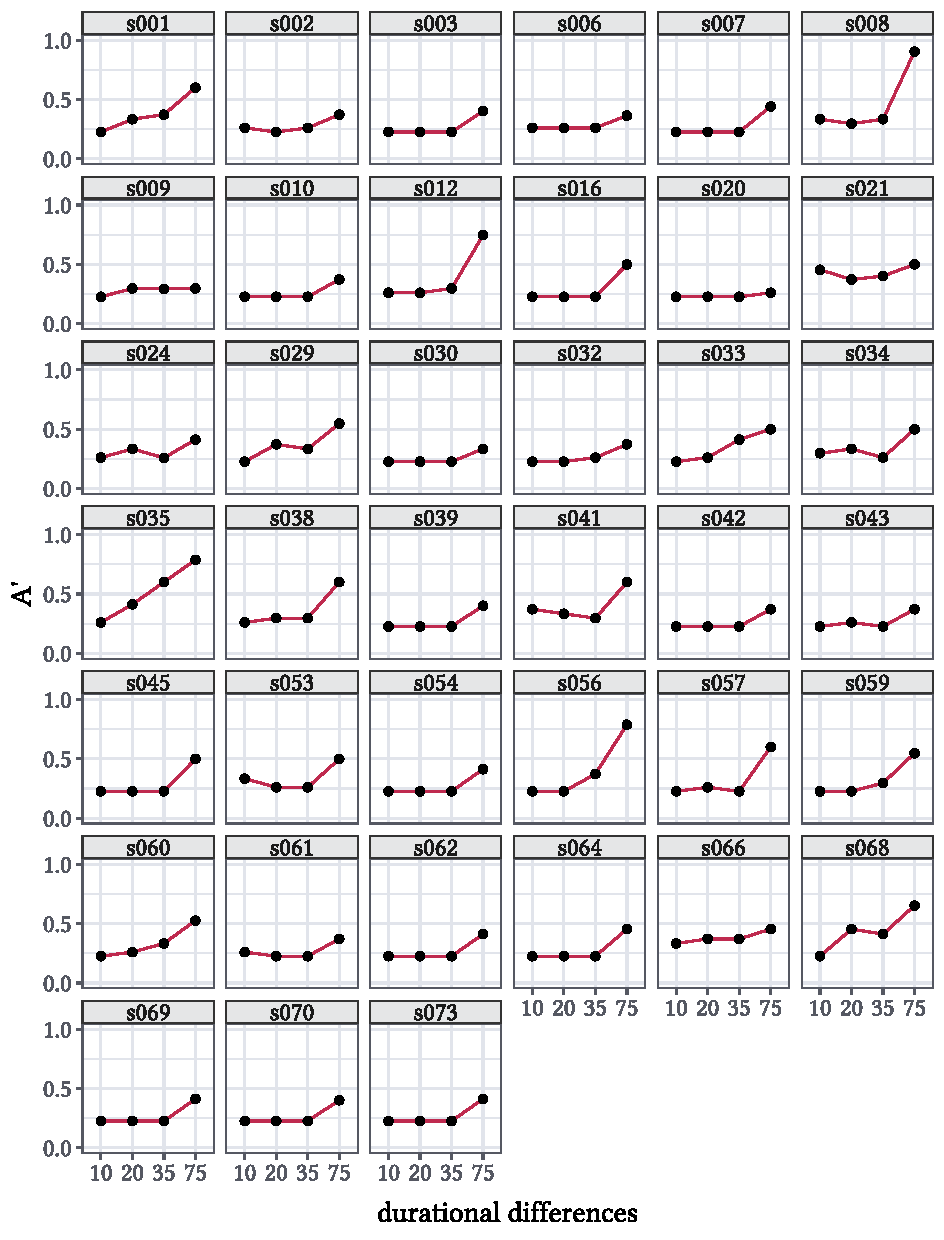
\includegraphics[width=1\textwidth]{figures/fig6.5.pdf}
    \caption{By-subject $A'$ values across all durational differences.}
    \label{fig:6_5}
\end{figure}

\section{Discussion}\label{section06_4}

Following previous studies on the perception of subphonemic differences, the present study investigated whether the durational differences between different types of word-final /s/ are perceptible. As such, this is the first study to look into the perception of phonologically identical but morphologically and phonetically different segments. Since real words as well as pseudowords were used as items, potential lexical effects were taken into account. It was found that durational differences in word-final /s/ as small as 10 ms and 20 ms are overall not well perceptible. Durational differences of 35 ms and 75 ms show significantly increased perceptibility, while a durational difference of 75 ms by far shows the greatest perceptibility.

What does this mean for the perceptibility of durational differences found for different types of word-final /s/? The durational differences found in \citet{Plag2017} and in the production study of Chapter \ref{chapter04} are given in Table \ref{tab:6.13}. None of the durational differences between the different types of /s/ is as high as 75 ms. However, considering the findings by \citet{Plag2017}, one would expect the differences between the non-morphemic /s/ and morphemic types of /s/ to be somewhat perceptible as these differences are all at least equal to or bigger than 35 ms. Taking into account the findings of Chapter \ref{chapter04}, only the durational difference between non-morphemic and clitic /s/ should be somewhat perceptible, as only this difference is close to or bigger than 35 ms. Considering both studies (\cite{Plag2017} and Chapter \ref{chapter04}), the findings indicate that at least some of the durational differences found between different types of /s/ are likely to be perceptible.

\begin{table}\fontsize{10}{11}
\caption{Durational differences between non-morphemic, plural, \mbox{is-,} and has-clitic /s/ in milliseconds found in \citet{Plag2017} and the production study presented in Chapter \ref{chapter04}.}
\label{tab:6.13}
\centering
\begin{tabular}{llcccc} 
\lsptoprule
\textbf{~}                           & ~           & non-morphemic & plural & \textit{is}-clitic & \textit{has}-clitic  \\ 
\midrule
\multirow{2}{*}{non-morphemic}       & Plag et al. & n.a.          & 35     & 57                 & 65                   \\
                                     & Chapter 4   & n.a.          & 14     & 31                 & 37                   \\ 
\midrule
\multirow{2}{*}{plural}              & Plag et al. & ~             & n.a.   & 22                 & 30                   \\
                                     & Chapter 4   & ~             & n.a.   & 17                 & 23                   \\ 
\midrule
\multirow{2}{*}{\textit{is}-clitic}  & Plag et al. & ~             & ~      & n.a.               & 8                    \\
                                     & Chapter 4   & ~             & ~      & n.a.               & 6                    \\ 
\midrule
\multirow{2}{*}{\textit{has}-clitic} & Plag et al. & ~             & ~      & ~                  & n.a.                 \\
                                     & Chapter 4   & ~             & ~      & ~                  & n.a.                 \\
\lspbottomrule
\end{tabular}
\end{table}

The significant increase in sensitivity of the 35 ms durational difference found in the present study is more or less in line with the findings by \citet{Klatt1975}. Recall that in their experiment, the just-noticeable difference to be perceived was 25 ms. That is, a durational difference between the 20 ms and 35 ms difference. The sensitivity between these two durational differences showed a significant increase, thus indicating that the just-noticeable difference to be perceived most likely lies within this range.

However, an overall increase in perceptibility was only found for the durational difference of 75 ms, for which the difference in sensitivity is significant for all comparisons. While I cannot give a definitive answer to the question of why this is the case, I want to propose two considerations. First, fricatives such as /s/ are not only perceived in terms of their duration but also by their centre of gravity, spectral peak location, spectral moments, noise duration, amplitude, and other acoustic features. In the present study, only one of many features – duration – was controlled for and manipulated. Perceptibility might be higher if all acoustic features are manipulated accordingly. Second, in their study, \citet{Klatt1975} found that durational differences in word-final position and in fricatives are less well perceptible as compared to other positions and consonants. As the present study investigated differences between fricatives in word-final position, perceptibility was expected to be rather low.

Let us now turn to the theoretical implications of the present results. How do the results relate to the two hypotheses that were tested? \textsc{H perc\textsubscript{1}}, the \textit{Abstractionist Hypothesis}, assumes that listeners are not sensitive to subphonemic durational differences. As was illustrated, listeners show an increased sensitivity towards a durational difference of 35 ms and such a difference in duration was found between different types of word-final /s/ (e.g. \cite{Plag2017}; Chapter \ref{chapter04}). Also, none of the tested durational differences distinguishes between phonemes of English: No matter what its acoustic duration within a reasonable range, an /s/ is an /s/. Thus, the \textit{Abstractionist Hypothesis} is rejected.

As listeners were sensitive to subphonemic durational differences, \textsc{H perc\textsubscript{2}}, the \textit{Phonetic Detail Hypothesis}, can potentially be confirmed. Assuming that fine-phonetic detail is perceived and stored, this hypothesis can most likely account for the present findings. Recent findings in neurobiology (\cite{Beach2021}) are especially compatible with the notion of hybrid models, as are part of this hypothesis. That is, brain response patterns in same-different tasks suggest that the perception process does not require loss of subphonemic detail. Instead, the neural representation of perceived speech includes phonemic and subphonemic detail. Yet, a final decision on whether theories underlying this hypothesis can account for the present findings can only be reached with pertinent implementations.

The results of the present study then give rise to a further question: Are durational differences between different types of word-final /s/ made use of in comprehension? This question will be investigated in Chapters \ref{chapter07} and \ref{chapter08}.

%\chapter{Comprehension of non-morphemic and plural /s/}\label{chapter07}

As illustrated in detail in Section \ref{section02_2}, two comprehension studies are part of this book. This chapter presents the first of these studies on the comprehension of subphonemic differences in word-final /s/. It makes use of real words in isolation with non-morphemic and plural word-final /s/ as items. Effects on comprehension were tested using a number-decision task in a mouse-tracking paradigm. Considering extant models and approaches of speech perception and comprehension, \textsc{H comp}, the \textit{Mismatch Hypothesis}, is investigated. That is, if listeners make use of subphonemic durational differences in the comprehension of different types of word-final /s/, then a mismatch of subphonemic detail and intended meaning is predicted to lead to a) slowed down comprehension processes, and b) deviated mouse trajectories. 

\section{Methdology}\label{section07_1}

\subsection{Participants}\label{section07_1_1}

Forty native speakers of New Zealand English took part in the experiment. They were the same participants who also participated in the same-different task described in Chapter \ref{chapter06}. As was the case for the perception experiment, one parti-cipant did not respond in any trials and was therefore excluded. The experiment took place at the University of Canterbury, Christchurch, New Zealand, from December 2020 to March 2021.

\subsection{Materials}\label{section07_1_2}

For the present experiment, only real words were used. Recall that words were taken from the British National Corpus (\cite{Davies2004}), following a number of criteria. That is, words had to have a word-final /s/ as part of a voiceless stop plus sibilant coda; they had to be either singular or plural nouns with one syllable; and the number of short monophthong, long monophthong, and diphthong nuclei had to be equally distributed across words for both singular and plural nouns. For singular /s/, it was not possible to fully meet the final criterion as there was only one word with a long monophthong nucleus. Another monomorphemic word with a short monophthong was used instead. As such words had already been sampled for the perception experiment in Chapter \ref{chapter06}, that set of words was used here as well. Additionally, six new words for both singular and plural nouns were added to increase the overall amount of data without a repetition of items (see \cite{Winter2021Grice}, on why repetitions are not desirable). Table \ref{tab:7.1} gives an overview of the complete set of words. As it was not possible to find more monomorphemic words with an even distribution of short monophthongs, long monophthongs, and diphthongs as nuclei, further monomorphemic words with a short monophthong nucleus were used instead.

\begin{table}\fontsize{10}{11}
\caption{Words used as items in the number-decision task. The upper half of words is identical to the set of words used in the perception experiment. The lower half of words was added for the present comprehension experiment.}
\label{tab:7.1}
\centering
\begin{tabular}{llll}
\lsptoprule
\multicolumn{2}{c}{Non-morphemic /s/} & \multicolumn{2}{c}{Plural suffix /s/}  \\
\midrule
item            & vowel quality       & item            & vowel quality        \\
\midrule
\textit{mix}    & short               & \textit{books}  & short                \\
\textit{box}    & short               & \textit{steps}  & short                \\
\textit{tax}    & short               & \textit{rights} & diphthong            \\
\textit{coax}   & diphthong           & \textit{points} & diphthong            \\
\textit{hoax}   & diphthong           & \textit{groups} & long                 \\
\textit{corpse} & long                & \textit{parts}  & long                 \\
\hline
\textit{lynx}   & short               & \textit{costs}  & short                \\
\textit{flux}   & short               & \textit{crusts} & short                \\
\textit{wax}    & short               & \textit{rates}  & diphthong            \\
\textit{fax}    & short               & \textit{notes}  & diphthong            \\
\textit{lapse}  & short               & \textit{sports} & long                 \\
\textit{fox}    & short               & \textit{cheats} & long                \\
\lspbottomrule
\end{tabular}
\end{table}

The set of twenty-four target items was matched with a set of twenty-four filler items. Half of the filler items were high frequency monosyllabic singular words ending in any consonant but /s/. The other half of the filler items were disyllabic plurals ending in /ɪz/. The type of nucleus, i.e. short or long monophthong and diphthong, was distributed equally across both groups of fillers. All fillers used in the present experiment can be found in Table \ref{tab:7.2}.

\begin{table}\fontsize{10}{11}
\caption{Filler items used in the number-decision task.}
\label{tab:7.2}
\centering
\begin{tabular}{llll}
\lsptoprule
\multicolumn{2}{c}{High frequency singulars} & \multicolumn{2}{c}{/ɪz/ plurals}  \\
\midrule
item  & vowel quality                        & item    & vowel quality           \\
\midrule
\textit{end}   & short                                & \textit{kisses}  & short                   \\
\textit{fact}  & short                                & \textit{fences}  & short                   \\
\textit{head}  & short                                & \textit{passes}  & short                   \\
\textit{thing} & short                                & \textit{senses}  & short                   \\
\textit{home}  & diphthong                            & \textit{roses}   & diphthong               \\
\textit{point} & diphthong                            & \textit{houses}  & diphthong               \\
\textit{way}   & diphthong                            & \textit{bases}   & diphthong               \\
\textit{side}  & diphthong                            & \textit{spices}  & diphthong               \\
\textit{car}   & long                                 & \textit{classes} & long                    \\
\textit{world} & long                                 & \textit{horses}  & long                    \\
\textit{room}  & long                                 & \textit{nurses}  & long                    \\
\textit{court} & long                                 & \textit{uses}    & long                   \\
\lspbottomrule
\end{tabular}
\end{table}

The recording of the speech materials took place at a soundproof booth of the Department of Linguistics at the University of Tübingen. For the recording procedure, reading lists were created. On these lists, target items were embedded within the sentence ``He said \textit{item} to me.", while filler items were embedded within the sentence ``He said \textit{item} again.". The latter sentence was used for filler items as some of them ended in alveolar stops, /d/ and /t/. Thus, the word \textit{to} following the respective filler items would have potentially led to splicing problems later on due to coarticulatory effects, i.e. the omission of one of the two stops, between filler item and the following word. To keep differences due to phrasal context to a minimum, the decision was made to embed all filler items into the second sentence, including those without word-final alveolar stop. Target items were not embedded within the same sentence but within the one mentioned first, as for word-final /s/ a following stop simplifies the segmentation procedure due to the clear cut-off between friction and closure in the acoustic signal. Examples of target and filler items embedded in the pertinent sentences are given in \ref{ex:14:sentence14} and \ref{ex:15:sentence15}, respectively.

\ex.
\label{ex:14:sentence14}
He said \textit{hoax} to me.

\ex.
\label{ex:15:sentence15}
He said \textit{world} again.

A trained native speaker of New Zealand English read the entire reading list aloud for practice before recording the list three times. The recordings were sampled at 44.1 kHz, 16 bit. 

For each item the best of the three recordings was chosen by manual inspection. First, all recordings were analysed using Praat following the segmentation conventions laid out in Section \ref{section04_1_4}. Recordings with production errors, e.g. laughter, stutter or vocal fry, or segmentation difficulties, e.g. the absence of a stop release, were dismissed. Second, the remaining segmented items and filler items were spliced from their surrounding contexts, resulting in audio files only containing the words of interest. Third, the duration of the target and filler items was measured using a Praat script (\cite{deJong2008}) and then analysed in R. The result of this analysis is given as the mean durations presented in Table \ref{tab:7.3}. Lastly, the version closest to the mean duration of its nucleus type was chosen for further use in the experiment to keep durational differences between items to a minimum.

\begin{table}\fontsize{10}{11}
\caption{Mean durations of items and filler items across recordings in seconds.}
\label{tab:7.3}
\centering
\begin{tabular}{llccc} 
\lsptoprule
Item type                                                       & ~                                                                   & Short vowel                                           & Long vowel                                            & Diphthong                                              \\ 
\midrule
target items                                                    & \begin{tabular}[c]{@{}l@{}}\textit{mean} \\\textit{sd}\end{tabular} & \begin{tabular}[c]{@{}l@{}}0.576 \\0.109\end{tabular} & \begin{tabular}[c]{@{}l@{}}0.613 \\0.102\end{tabular} & \begin{tabular}[c]{@{}l@{}}0.572 \\0.062\end{tabular}  \\ 
\midrule
\begin{tabular}[c]{@{}l@{}}singular \\filler items\end{tabular} & \begin{tabular}[c]{@{}l@{}}\textit{mean} \\\textit{sd}\end{tabular} & \begin{tabular}[c]{@{}l@{}}0.469 \\0.082\end{tabular} & \begin{tabular}[c]{@{}l@{}}0.467 \\0.035\end{tabular} & \begin{tabular}[c]{@{}l@{}}0.523 \\0.071\end{tabular}  \\ 
\midrule
\begin{tabular}[c]{@{}l@{}}plural \\filler items\end{tabular}   & \begin{tabular}[c]{@{}l@{}}\textit{mean} \\\textit{sd}\end{tabular} & \begin{tabular}[c]{@{}l@{}}0.609 \\0.081\end{tabular} & \begin{tabular}[c]{@{}l@{}}0.607 \\0.056\end{tabular} & \begin{tabular}[c]{@{}l@{}}0.613 \\0.069\end{tabular}  \\
\lspbottomrule
\end{tabular}
\end{table}

Next, for each target the chosen recording was edited so that the word-final /s/ was replaced with another word-final /s/. For recordings of the so-called \textit{matched condition}, this new word-final /s/ was taken from another recording of the same word. If the /s/ was a non-morphemic /s/, its duration was manipulated in such a way that is corresponded to the mean non-morphemic /s/ duration found in \citet{Plag2017}. If the /s/ was a plural /s/, its duration was changed to the mean plural /s/ duration found in the same study, accordingly. For recordings of the so-called \textit{mismatched condition}, the new word-final /s/ was taken from a monomorphemic target in case of a plural base and from a plural target in case of a monomorphemic pseudo-base, i.e. the string of segments of a monomorphemic target without the word-final /s/. The duration of the /s/ was then manipulated in such a way that it corresponded to the mean duration found in \citet{Plag2017} for the other type of /s/. That is, a non-morphemic /s/ was changed to the duration of a plural /s/, and a plural /s/ was changed to the duration of a non-morphemic /s/. This procedure resulted in two recordings per target word, one of the matched condition and one of the mismatched condition. For example, for the monomorphemic target word \textit{mix}, there was an audio stimulus with an /s/ duration of 318 ms for the matched condition and an audio stimulus with an /s/ duration of 283 ms for the mismatched condition. For a plural target like \textit{books}, there was an audio stimulus with an /s/ duration of 283 ms for the matched condition and an audio stimulus with an /s/ duration of 318 ms for the mismatched condition. As the (pseudo-)base and the /s/ in both conditions have been spliced together, a one-sided effect of ``sounding manipulated" on the experiment’s results was ruled out.

In sum, each participant completed 72 trials, i.e. 12 matched non-morphemic /s/ items + 12 matched plural /s/ items + 12 mismatched non-morphemic /s/ items + 12 mismatched plural /s/ items + 12 high frequency singular items + 12 /ɪz/ plural items.

\subsection{Procedure}\label{section07_1_3}

The number-decision task was conducted in OpenSesame using the \texttt{mousetrap} plugin for mouse-tracking (\cite{Kieslich2017}). Participants were introduced to the task at hand. They were told that in the following experiment they had to decide whether an audio recording was describing ``one" or ``two or more" entities. They were told to mouse-click on the corresponding button in the top right or top left corner of the screen as quickly as possible. Figure \ref{fig:7_1} illustrates what participants saw on screen for each trial. The participants were also told that if they did not decide on either option within a certain amount of time, the next trial would start automatically. Each participant started with six practice trials in which recordings of filler items were used (see the supplementary material given in Chapter \ref{Supplementary Material}).

\begin{figure}
    \centering
    \includegraphics[width=0.7\textwidth]{figures/fig7.1.png}
    \caption{Option display during the comprehension experiment. The mouse cursor indicates the position the mouse was reset to in each trial.}
    \label{fig:7_1}
\end{figure}

Each trial was preceded by a stretch of silence of 450 ms. Then, one of the recordings was played, with reaction time and mouse-tracking measurement starting at the onset of the recording. Participants were given a window of 2000 ms starting after the onset of the recording to react, after that a time-out was recorded. The next trial started automatically 2500 ms after the onset of the recording if no reaction was recorded. Mouse-tracks were recorded with a frequency of 100 Hz.

\section{Analysis}\label{section07_2}

The data of the mouse-tracking experiment were analysed in terms of reaction times and mouse trajectories. In the following section, covariates used in the analyses are introduced. Section \ref{section07_2_2} then presents the analysis of reaction time data. The analysis of the mouse-tracks is given in Section \ref{section07_2_3}.

\subsection{Covariates}\label{section07_2_1}

The set of covariates used in the analyses of the present study is similar to that of other studies on phonetic effects of morphological structure (\cite{Pluymaekers2005a, Pluymaekers2005b, Hanique2013Ernestus, Plag2017}; as well as those used in previous chapters of this book). Additionally, some further covariates, which may either influence perception or reactions based on perception, have been introduced. In the following, covariates based on previous studies on morphological structure are described first. For covariates which have been introduced in detail in Chapters \ref{chapter04} and \ref{chapter06}, definitions are briefly repeated for convenience and adapted where necessary. Then, newly introduced covariates are given. Finally, covariates used as random effects are listed.

\textsc{biphoneProbSum}. A covariate based on the summed biphone probability was used as a measure of contextual predictability.

\textsc{monoMultilingual}. To account for potential influences of other L1s besides English, the binary covariate \textsc{monoMultilingual} was introduced. 

\textsc{age}. Subjects’ \textsc{age} was included as it may show an influence on reaction times, with older subjects generally reacting slower than younger subjects (e.g. \cite{Fozard1994}).

\textsc{neighbourhoodDensity}. Neighbourhood densities were included as covariate as the number of neighbours may influence phonetic reduction (e.g. \cite{Gahl2012}). The measure was created using the CLEARPOND database (\cite{Marian2012}). \textsc{neighbourhoodDensity} describes the number of words differing in one segment from the item in question (\cite[3]{Marian2012}).

\textsc{trialNumer}. To account for possible effects of training and fatigue, the number of the trial during the experiment for each of the items per subject was included. 

\textsc{googleFreqLog}. To account for potential effects of frequency (e.g. \cite{Baayen2006, Keuleers2010, Brysbaert2011}), Google frequency was included as covariate as it has been shown that Google frequencies are a robust predictor of reaction times (e.g. \cite{Hendrix2020}). The value of \textsc{googleFreqLog} is the log-transformed number of Google search hits for each individual item as obtained on July 16, 2021.

\textsc{typeOfS}. This binary variable codes whether the pertinent pseudoword is a singular or plural form. It takes the value \texttt{nm} for pseudowords with a non-morphemic word-final /s/ and \texttt{pl} for pseudowords with a plural word-final /s/.

\textsc{musicalInstrument}. It has been shown that advanced players of musical instruments show an increased performance of phonological perception and of detecting durational differences in speech (\cite{Anvari2002, Milovanov2009}). Thus, information on how regularly each subject plays a musical instrument was added as covariate.

\textsc{condition}. The \textsc{condition} variable is the explanatory variable of interest. Its levels are matched and mismatched and refer to the \textit{matched} and \textit{mismatched} conditions introduced by the creation of the audio stimuli. Recall from Section \ref{section07_1_2} that in matched stimuli (pseudo-)base and duration of the word-final /s/ match up, while there is a discrepancy of (pseudo-)base and word-final /s/ duration for mismatched stimuli. 

\textsc{correct}. \textsc{correct} is a binary variable coding whether the answer clicked on by the subject in the relevant trial is the correct answer regarding the stimulus' (pseudo-)base.

\textsc{dominantHand}. Reaction times between the dominant and the non-domi-nant hand may differ (\cite{Gignac2004}). The information of which hand was dominant in each subject was added as a covariate, as all participants used the same hand (i.e. their right hand) to use the mouse.

\textsc{order}. This variable codes the order of X and Y coordinates, i.e. their chronological order in the observed mouse-tracks. \textsc{order} was incorporated as a variable to account for the natural sequence of coordinates, i.e. to account for potential influences of auto-correlation. 

\textsc{videoGames}. It has been shown that playing video games can reduce reaction times (e.g. \cite{Dye2009}). The relative frequency of how often a subject engages in playing video games was therefore included as a categorical covariate called \textsc{videoGames}.

\textsc{item}. For each item, its orthographic representation was contained as level of item. This covariate was used as a random effect to account for potential differences between individual targets not covered by other covariates.

\textsc{subject}. \textsc{subject} ID was included to account for inter-speaker differences in perception.

Closer inspection of the covariates describing subject characteristics, i.e. \textsc{dominantHand}, \textsc{monoMultilingual}, \textsc{musicalInstrument}, and \textsc{videoGames}, revealed that for all of these variables there was an uneven distribution of subjects across levels. That is, only 7\% (n = 117) of trials had \texttt{left} for \textsc{dominantHand}, and only 19\% (n = 302) of trials had \texttt{multilingual} for \textsc{monoMultilingual}. For \textsc{musicalInstrument} and \textsc{videoGames}, which both have five levels, the distribution is even more uneven. The level least represented in \textsc{musicalInstrument} is \texttt{very often} with 6\% (n = 95), while the most represented level is \texttt{never} with 41\% (n = 666). A similar picture is found for \textsc{videoGames}, where the least represented level is \texttt{often} with 8\% (n = 126), while the level most represented is \texttt{never} with 38\% (n = 621). The uneven distribution of data points across variables and their levels also led to some ``empty cells" within the possible combinations of levels across covariates. For example, all subjects for which the value of \textsc{monoMultilingual} is \texttt{multilingual} have \texttt{right} as their \textsc{dominantHand}. There are no \texttt{multilingual} subjects who play a musical instrument \texttt{often} or \texttt{very often} and no \texttt{multilingual} subjects who \texttt{often} play \textsc{videoGames}. Further, all \texttt{left}-handed subjects \texttt{never} play a \textsc{musicalInstrument} and they \texttt{rarely} or \texttt{never} play \textsc{videoGames}. Due to this issue of sparse data and as for such variables with levels underrepresented in the sample it is unclear whether effects, found or not found, are due to a real effect of the variable or simply an artefact of chance. It was thus decided to drop the following covariates: \textsc{dominantHand}, \textsc{musicalInstrument}, and \textsc{videoGames}. \textsc{monoMultilingual} is retained for the analyses as the variable is directly related to language and because the variable has been used in other analyses of this book.

\subsection{Reaction times}\label{section07_2_2}

The present reaction time data were analysed using piece-wise additive mixed models (PAMMs; \cite{Bender2018etal}, and as briefly introduced in Section \ref{section03_2_2}). In the following, I will introduce the basics of PAMMs; the interested reader is referred to \citet{Hendrix2020} for a more thorough introduction using linguistic data and to \citet{Bender2018etal} for a more detailed mathematical implementation. 

PAMMs are a relatively novel technique of time-to-event analysis, that is they model the time until an event of interest occurs. The event of interest in the present number-decision task is the ``one" or ``two or more" response to a stimulus. Thus, the dependent variable in a PAMM is the instantaneous probability of a response as it evolves over time, not the reaction time itself (\cite{Hendrix2020}). Using PAMMs allows for an insight into the temporal dynamics of predictor effects. Hence, PAMMs do not only capture effects covering entire trials but also effects that occur only during particular parts of trials or show different effects during different parts of trials. A central function of time-to-event analysis is the probability density function $F(t$):

\begin{equation}
\label{eq:Ft}
    F(t)=\int_{-\infty}^{t}f(x)dx=P(T\leq t).
\end{equation}

The probability density function describes the probability that the response time $T$ is smaller than or equal to a given time $t$. Closely related to the probability density function is the survival function:

\begin{equation}
\label{eq:St}
    S(t)=1-F(t)=P(T>t).
\end{equation}

The survival function describes the probability of the time at which the event of interest occurs, $T$ being greater than at a given time $t$. For the present experiment, the survival function describes the probability that subjects did not yet respond to a stimulus at time $t$. However, the mathematical properties of the function are not optimal for modelling purposes (\cite{Hendrix2020}). Thus, PAMMs make use of a closely related function, the hazard function. The hazard function describes the instantaneous probability that the event of interest occurs at time $t$, given that the event did not occur already. It is defined as

\begin{equation}
\label{eq:lambdat}
\lambda(t)=\lim \limits_{dt \to \infty}\frac{P(t\leq T\leq t\, |\, T\geq t)}{dt}=-\frac{d}{dt}log(S(t)).
\end{equation}

Before one can create PAMMs on reaction time data, though, the data have to be transformed. That is, the modelling of PAMMs requires data in the so-called piece-wise exponential data format (\cite{Bender2018a}). While standard linear models (e.g. LMERs) or non-linear regression models (e.g. GAMMs) would use reaction times as dependent variable, PAMMs use the information on whether or not a stimulus was responded to at time $t$ as dependent variable. The piece-wise exponential data format splits the time each stimulus is at risk of being responded to into $J$ intervals. The intervals $(k_{j-1},k_j ],j=1…J$ are defined by the cut points $K_0<⋯<K_J$. The choice of cut points is arbitrary (\cite{Hendrix2020}); over-fitting is prevented through penalisation of wiggliness (e.g. \cite{Wood2017}). $t_j$ then equals $k_j$, i.e. $t$ is derived from the defined cut points $K$. Following \citet{Hendrix2020}, cut points at the extreme ends of the response time distribution were opted for. That is, cut points prior 770 ms, as only 11 trials (0.68\%) were responded to earlier than 770 ms after stimulus onset, and after 1970 ms, as only 12 trials (0.74\%) were responded to later than 1970 ms after stimulus onset, were excluded. An example of the transformed data is given in Table \ref{tab:7.4}.

\begin{table}\fontsize{10}{11}
\caption{Example of the piece-wise exponential data format for one stimulus instantiating the word \textit{box}.}
\label{tab:7.4}
\centering
\begin{tabular}{lllrrrrr} 
\lsptoprule
row & \textsc{ID}  & \textsc{item} & \textsc{tstart}  & \textsc{tend}    & \textsc{interval}          & \textsc{offset} & \textsc{status}  \\ 
\midrule
1   & 256 & box  & 0.00    & 817.00  & (0.00,817]        & 6.706  & 0       \\
2   & 256 & box  & 817.00  & 922.00  & (817.00,922.00]   & 4.654  & 0       \\
3   & 256 & box  & 922.00  & 977.00  & (922.00,977.00]   & 4.007  & 0       \\
…   & …   & …    & …       & …       & …                 & …      & …       \\
26  & 256 & box  & 1345.92 & 1363.00 & (1345.92,1363.00] & 2.838  & 0       \\
27  & 256 & box  & 1363.00 & 1379.08 & (1363.00,1379.08] & 2.079  & 1       \\
\lspbottomrule
\end{tabular}
\end{table}

The piece-wise exponential data format contains a separate row for each interval for each stimulus. In each row, the start (\textsc{tstart}) and end point (\textsc{tend}) of the interval are given. The end points are included as predictor in a PAMM to estimate the hazard function over time. The \textsc{offset} variable provides information about the exact response time for each stimulus. For intervals in which no response was recorded (rows 1 to 26), the \textsc{offset} is the log-transformed duration of the interval, while for intervals in which a response was recorded (row 27), the \textsc{offset} is the log-transformed value of the difference of the exact time of response and the start of the interval, i.e. \textsc{tstart}. Please note the notation of the interval information: $(k_{j-1},k_j]$ indicates that the first value, $k_{j-1}$, is included in the interval while the second value, $k_j$, is not. $k_j$, then, is the starting value of the following interval. The dependent variable in PAMMs, \textsc{status}, is a binary variable, which encodes whether a word was responded to (\texttt{1}) or not (\texttt{0}) in the pertinent interval. 

A PAMM is then defined as follows:

\begin{equation}
\label{eq:lambdatxi}
\lambda(t|x_{i})=\lambda_{0}(t_{j})exp\left ( \sum_{k=1}^{p}f_{k}(x_{i,k},t_{j})+b_{\ell_{i}} \right ),\: \forall\, t \in (K_{j-1},K_{j}]
\end{equation}

\noindent with the predictor values $x_i$ for stimulus $i$ defining the hazard function $\lambda(t|x_{i})$ at all time points $t$ in the interval $j≔(K_{j-1},K_j]$. $λ_0 (t_j)$ is the baseline hazard for time interval $j$, $f_k (x_{i,k},t_j)$ are smooth functions for predictor $k∈1,…,p$ for each time point $t$ in the interval $j$, and $b_{\ell_{i}}$ are random intercepts associated with group $l∈1,…,L$ to which stimulus $i$ belongs (\cite{Hendrix2020}).

\subsubsection{Overview of the data}\label{section07_2_2_1}

An overview of all variables used in the PAMM modelling process and their distribution is given in Table \ref{tab:7.5} and Table \ref{tab:7.6}.

\begin{table}\fontsize{10}{11}
\caption{Summary of the dependent variable and the numerical predictors in the final data set.}
\label{tab:7.5}
\centering
\begin{tabular}{lrrrr} 
\lsptoprule
Dependent variable   & \multicolumn{4}{l}{Levels}                                      \\ 
\midrule
\textsc{status}               & \multicolumn{2}{l}{0:
  41471} & \multicolumn{2}{l}{1:
  1616}  \\ 
\midrule
Numerical predictors & Mean     & St. Dev.            & Min     & Max                  \\ 
\midrule
\textsc{biphoneProbSum}       & 0.015    & 0.009               & 0.002   & 0.043                \\
\textsc{age}                  & 23.313   & 5.575               & 18.000  & 39.000               \\
\textsc{neighbourhoodDensity} & 17.068   & 10.039              & 1.000   & 34.000               \\
\textsc{trialNumber}          & 36.358   & 20.678              & 1.000   & 72.000               \\
\textsc{googleFreqLog}        & 9.190    & 0.787               & 7.658   & 10.302               \\
\textsc{tend}                 & 1234.455 & 212.414             & 817.000 & 1960.000             \\
\lspbottomrule
\end{tabular}
\end{table}





\begin{table}\fontsize{10}{11}
\caption{Summary of the categorical predictors and the explanatory variable in the final data set.}
\label{tab:7.6}
\centering
\begin{tabular}{lllll} 
\lsptoprule
Categorical predictors & Levels & ~                               & ~ & ~                                     \\ 
\midrule
\textsc{typeOfS}                & \multicolumn{2}{l}{\texttt{nm}: 22159}            & \multicolumn{2}{l}{\texttt{pl}:
  20928}           \\
\textsc{correct}                & \multicolumn{2}{l}{\texttt{no}: 7795}             & \multicolumn{2}{l}{\texttt{yes}: 35292}            \\
\textsc{monoMultilingual}       & \multicolumn{2}{l}{\texttt{monolingual}:
  37578} & \multicolumn{2}{l}{\texttt{multilingual}:
  5509}  \\
\textsc{item}                   & 24     & ~                               & ~ & ~                                     \\
\textsc{subject}                & 39     & ~                               & ~ & ~                                     \\ 
\midrule
Explanatory variable   & Levels & ~                               & ~ & ~                                     \\ 
\midrule
\textsc{condition}              & \multicolumn{2}{l}{\texttt{matched}:
  21176}     & \multicolumn{2}{l}{\texttt{mismatched}:
  21911}   \\
\lspbottomrule
\end{tabular}
\end{table}

\subsubsection{Fitted models}\label{section07_2_2_2}

A PAMM was fitted with \textsc{status} as dependent variable and \textsc{biphoneProbSumBin}, \textsc{age}, \textsc{neighbourhoodDensity}, \textsc{trialNumer}, and \textsc{googleFreqLog} as smooth terms. For each smooth, time-varying predictor effects were allowed for by including tensor product interactions between time, i.e. \textsc{tend}, and the predictor itself (see \cite{Wood2017}, for further details on tensor product interactions). To ensure interpretable results, the predictor smooths were limited to four basis functions, and time-by predictor interactions were limited to fourth order non-linearities. No limits were set on the smooth for time. The categorical covariates \textsc{typeOfS}, \textsc{condition}, \textsc{correct}, and \textsc{monoMultilingual} were included as parametric effects. The covariates \textsc{item} and \textsc{subject} were included as random smooth terms. Starting from this initial model, the modelling process proceeded as introduced in Section \ref{section03_2_2}. It was found that the \textit{k}-index value of the tensor product interaction of \textsc{tend} and \textsc{trialNumber} was $0.006$. Recall that \textit{k}-values well below $0.05$ indicate potentially missed patterns in the residuals. Re-modelling with a limit of a sixth instead of a fourth order non-linearity resolved the issue. The prediction error curve (e.g. \cite{Mogensen2012}) displaying the Brier score (e.g. \cite{Brier1950, Gerds2006, Bradley2008}) of the final model is displayed in Figure \ref{fig:7_2}. As a reference, the Brier score of the Kaplan-Meier estimate (\cite{Kaplan1958}) is given. The Brier score measures the accuracy of probabilistic predictions. The lower its value for a set of predictions, the better the predictions are calibrated. The range of possible Brier score values is $(0,1)$. In the present case, the Brier score of the PAMM is considerably better than the Brier score of the Kaplan-Meier estimate. This indicates that the inclusion of the covariates in the PAMM improves the accuracy of the model predictions. 

\begin{figure}
    \centering
    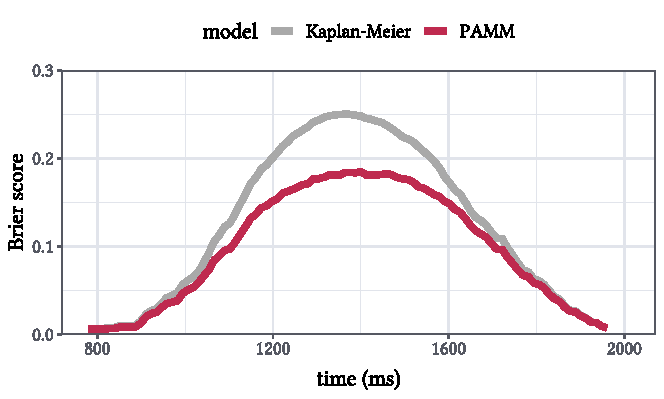
\includegraphics[]{figures/fig7.2.pdf}
    \caption{Comparison of the Brier scores of the fitted PAMM and its Kaplan-Meier estimate equivalent.}
    \label{fig:7_2}
\end{figure}

A valid question to ask when using novel statistical methods is whether the extra work is worth the trouble, i.e. whether the novel methods result in, for example, models with a higher fit. To answer this question for the present case, an LMER model with reaction time as dependent variable was fitted. As fixed effects, the parametric effects and smooth terms given in the PAMM formula (i.e. \textsc{biphoneProbSum, age, neighbourhoodDensity, trialNumber, googleFreqLog, typeOfS, condition, correct} and \textsc{monoMultilingual}) were specified. \textsc{item} and \textsc{subject} were included as random intercepts. The modelling process then followed the procedure introduced in Section \ref{section03_2_1}. The final LMER model and the PAMM model were then compared by their AIC values: The AIC value of the LMER model was $21,811.36$, the AIC value of the PAMM was $15,360.92$. That is, the AIC value of the PAMM was smaller by $6,450.438$ points. Thus, the PAMM shows a significantly better fit. Regarding its model formula, the final LMER model only contained \textsc{trialNumber} and \textsc{monoMultilingual} as fixed effects and \textsc{subject} as random effect. To briefly foreshadow the results presented in the next section, the LMER model did not find a significant effect for \textsc{age}, while the PAMM did find a significant interaction of \textsc{age} and time (\textsc{tend}). This difference then denotes the potentially most prominent advantage of PAMMs: As mentioned in Section \ref{section07_2_2}, PAMMs allow for an insight into the temporal dynamics of predictor effects, while LMER models fitted to the raw reaction time data do not. Overall, fitting PAMMs instead of LMER models appears to be worthwhile for the present data.

\subsubsection{Results}\label{section07_2_2_3}

Main effects of the following predictors were found: \textsc{tend}, \textsc{trialNumber}, and \textsc{monoMultilingual}. Additionally, the interactions between \textsc{tend} and \textsc{trial} and between \textsc{tend} and \textsc{age} reached significance. The results of the PAMM fitted to the reaction time data are given in Table \ref{tab:7.7}. For the parametric terms, I provide the β estimates and the corresponding standard errors (SE), \textit{z}-values, and \textit{p}-values. For the smooth terms, the estimated degrees of freedom, the reference degrees of freedom, the χ\textsuperscript{2} values, and the \textit{p}-values are given. The R script used for the analyses as well as the data set can be found in the supplementary material given in Chapter \ref{Supplementary Material}.

\begin{table}\fontsize{10}{11}
\caption{Summary of the PAMM fitted to status with \textsc{typeOfS}, \textsc{condition}, \textsc{correct}, and \textsc{monoMultilingual} as parametric effects, \textsc{biphoneProbSum}, \textsc{age}, \textsc{NeighbourhoodDensity}, \textsc{trialNumber}, and \textsc{GoogleFreqLog} as smooth terms, and \textsc{item} and \textsc{subject} as random smooth terms.}
\label{tab:7.7}
\centering
\begin{tabular}{lrrrr} 
\lsptoprule
Parametric Terms             & Estimate & SE     & z value  & \textit{p}-value  \\ 
\midrule
(Intercept)                  & -6.867   & 0.152  & -45.238  & 0.000             \\
\textsc{typeOfS}\texttt{pl}                    & 0.133    & 0.101  & 1.321    & 0.187             \\
\textsc{monoMultilingual}\texttt{multilingual} & 0.788    & 0.302  & 2.614    & 0.009             \\
\textsc{condition}\texttt{mismatched}          & -0.044   & 0.051  & -0.858   & 0.391             \\
\textsc{correct}\texttt{yes}                   & 0.061    & 0.075  & 0.810    & 0.418             \\ 
\midrule
Smooth Terms                 & edf      & Ref.df & Chi.sq   & \textit{p}-value  \\ 
\midrule
\textsc{tend}                         & 7.830    & 8.653  & 1516.374 & 0.000             \\
\textsc{GoogleFreqLog}                & 1.002    & 1.003  & 0.468    & 0.682             \\
\textsc{biphoneProbSum}               & 1.001    & 1.002  & 0.989    & 0.321             \\
\textsc{NeighbourhoodDensity}         & 1.300    & 1.495  & 1.760    & 0.391             \\
\textsc{age}                          & 1.002    & 1.002  & 3.258    & 0.071             \\
\textsc{trialNumber}                  & 1.001    & 1.002  & 64.063   & 0.000             \\ 
\midrule
Interactions                 & edf      & Ref.df & Chi.sq   & \textit{p}-value  \\ 
\midrule
\textsc{tend,
  GoogleFreqLog}        & 1.352    & 1.613  & 0.580    & 0.753             \\
\textsc{tend,
  biphoneProbSum}       & 1.539    & 1.882  & 1.238    & 0.423             \\
\textsc{tend,
  NeighbourhoodDensity} & 1.016    & 1.031  & 1.215    & 0.281             \\
\textsc{tend,
  age}                  & 5.942    & 7.321  & 20.257   & 0.007             \\
\textsc{tend,
  trialNumber}          & 2.982    & 3.012  & 50.727   & 0.000             \\ 
\midrule
Random Smooth Terms          & edf      & Ref.df & Chi.sq   & \textit{p}-value  \\ 
\midrule
\textsc{item}                         & 3.112    & 20.000 & 3.879    & 0.267             \\
\textsc{subject}                      & 34.184   & 36.000 & 505.162  & 0.000             \\
\lspbottomrule
\end{tabular}
\end{table}

Figure \ref{fig:7_3} shows the distribution of raw reaction times for items in the matched and mismatched \textsc{condition}. On average, matched stimuli are reacted to after 1374 ms, while mismatched stimuli are reacted to after 1388 ms. 

\begin{figure}
    \centering
    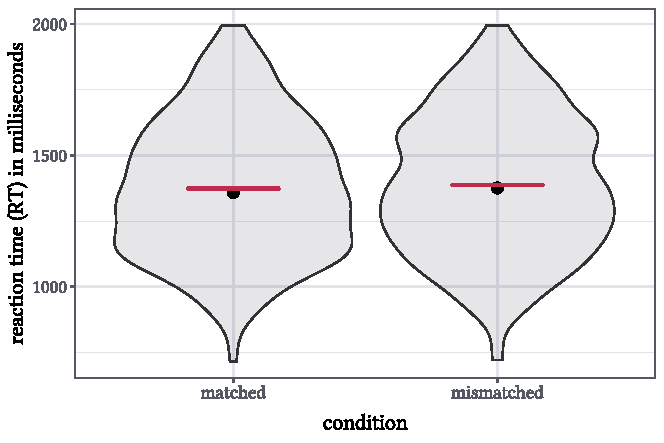
\includegraphics[]{figures/fig7.3.pdf}
    \caption{Observed reaction times for trials of matched and mismatched items. The dot represents the median, the horizontal line indicates the mean. The violin shapes represent rotated density plots describing the distribution of the data.}
    \label{fig:7_3}
\end{figure}

Taking into account this rather small difference of 14 ms and the overall similarity of shape between the two RT distributions, it is not surprising that \textsc{condition} as a predictor did not reach significance in the PAMM. The significant effects found instead are explained in the following.

Panel A of Figure \ref{fig:7_4} shows the partial effect ($p<0.001$) of the categorical variable \textsc{monoMultilingual}. It is found that \texttt{multilingual} subjects show a higher probability of earlier responses than \texttt{monolingual} subjects. This effect is visible in the distribution of the raw RT data (Panel B) as well. However, one should take this effect with caution as the number of \texttt{multilingual} subjects’ data points (n = 302) is much smaller than the number of \texttt{monolingual} subjects’ data points (n = 1326). 

\begin{figure}
    \centering
    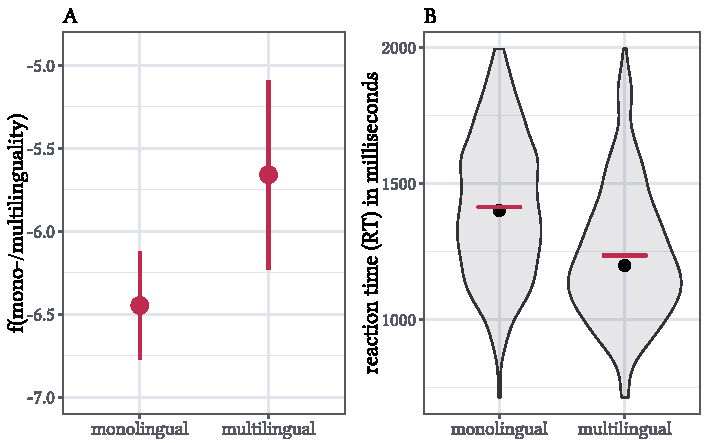
\includegraphics[]{figures/fig7.4.pdf}
    \caption{Partial main effect of \textsc{monoMultilingual} (A), and observed reaction times for monolingual and multilingual subjects (B).}
    \label{fig:7_4}
\end{figure}

A significant main effect of \textsc{trialNumber} ($χ^{2}=63.890, p<0.001$) was found, as well as a significant interaction between time and \textsc{trialNumber} ($χ^{2}=50.205,$ $p<0.001$). The effect of \textsc{trialNumber} is modulated by the interaction with time as shown in Figure \ref{fig:7_5}. Warmer colours indicate higher hazard rates.\footnote{Note that readers of a black and white version of this book should rely on the numbers on the lines instead. Warmer colours correspond to positive values, while cooler colours correspond to negative values.} That is, the interaction between \textsc{trialNumber} and time indicates that the increase of the instantaneous probability of a response for later trials is especially prominent during the early stages of the response window. Later on, the facilitatory main effect of \textsc{trialNumber} is offset by an opposite effect of the partial interaction between \textsc{trialNumber} and time.

\begin{figure}
    \centering
    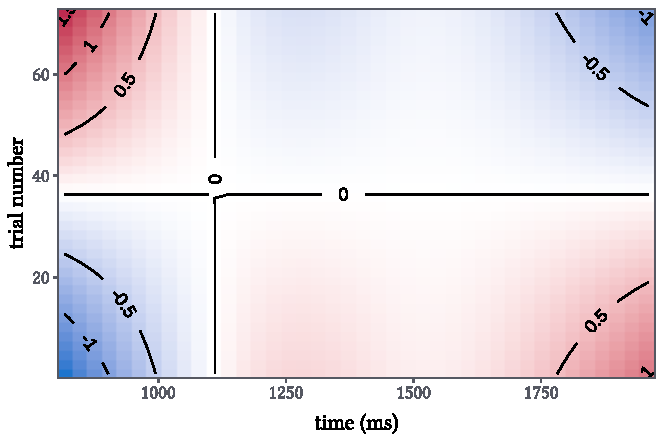
\includegraphics[]{figures/fig7.5.pdf}
    \caption{The effect of the interaction between \textsc{trialNumber} and time. Warmer colours indicate higher hazard rates.}
    \label{fig:7_5}
\end{figure}

Finally, a significant interaction between time and \textsc{age} ($χ^{2}=20.151, p<0.05$) was found. This effect is illustrated in Figure \ref{fig:7_6}. Again, warmer colours indicate higher hazard rates. That is, the interaction between \textsc{age} and time indicates that the increase of the instantaneous probability of a response for ages between approximately 23 and 28 years is especially prominent during the mid to late stages of the response window, i.e. around 1400 ms to 1750 ms into the trial. The grey area indicates ranges for which no or not enough data were available to the model.\footnote{For readers of a black and white version of this book this area should be visible as dark grey area, which is almost shaped like a perfect rectangle.} As only few subjects (n = 4) contribute to the data above the grey area, shown effects should be interpreted with caution. 

\begin{figure}
    \centering
    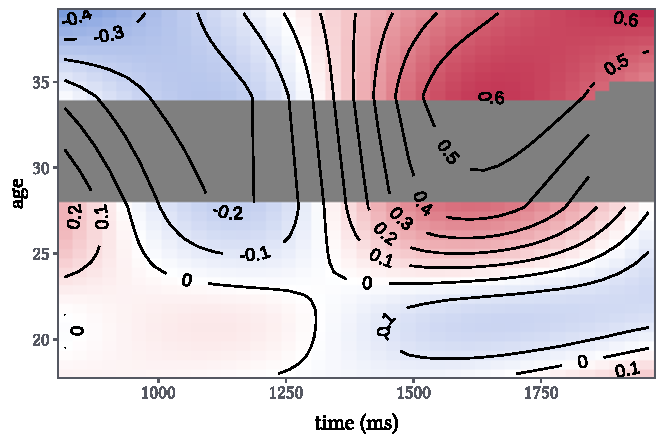
\includegraphics[]{figures/fig7.6.pdf}
    \caption{The effect of the interaction between \textsc{age} and time. Warmer colours indicate higher hazard rates.}
    \label{fig:7_6}
\end{figure}

\subsubsection{Interim summary: Reaction times}\label{section07_2_2_4}

Overall, \textsc{condition} as a predictor did not reach significance in the PAMM. That is, participants responded with the same speed to matched and mismatched items. Instead, effects of \textsc{monoMultilingual}, \textsc{trialNumber}, and \textsc{age} were found.

\subsection{Mouse-tracks}\label{section07_2_3}

Mouse-tracking data elicited in OpenSesame using the \texttt{mousetrap} plugin (\cite{Kieslich2017}) were worked with in R using the \texttt{mousetrap} package (\cite{Kieslich2019}). Following standard procedures, the raw mouse-tracking data were first transformed to the so-called \textit{mousetrap data format} using the \texttt{mt\_import\_mousetrap} function. This function transforms the vectors of X and Y coordinates and their associated timestamps into meaningful row-by-row data for further processing. Then, trials without mouse-movement were discarded. During the experiment subjects clicked on the right and left options on screen (see Section \ref{section07_1_3}). To make mouse-tracks to both sides comparable, those towards the right option were mirrored vertically. Finally, all mouse-tracking data were time-normalised. Time-normalisation is commonly performed if the number of recorded X and Y coordinates varies across trajectories, which typically is the case for trajectories of differing reaction times. After time-normalisation with a constant number of equally sized time steps, all trajectories have the same number of recorded positions, and the positions at different relative time points can be compared across trajectories. 

Figure \ref{fig:7_7} shows the mean trajectory of all spatially adjusted and time-norma-lised mouse-tracks used in the present analysis in the lower left panel. The panel on top displays the overall distribution of all X coordinates, with a clear peak around a value of $0$. The panel on the right shows the overall distribution of all Y coordinates, with a clear peak around a value of about $380$. The peaks correspond to the position to which the mouse was reset to for each trial.

\begin{figure}
    \centering
    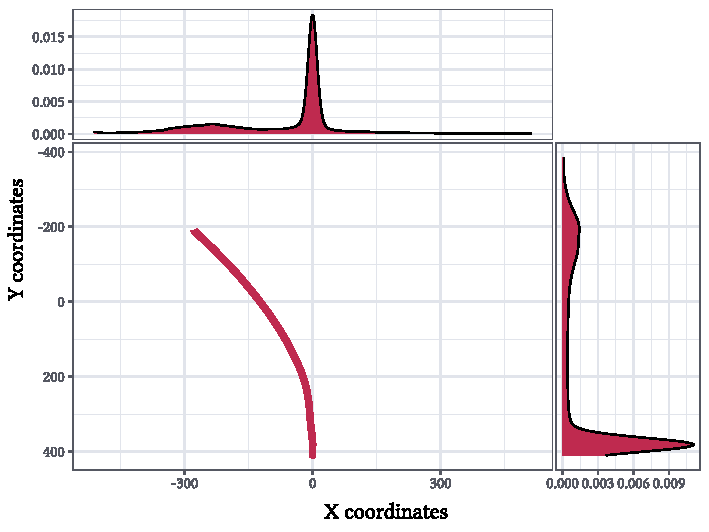
\includegraphics[]{figures/fig7.7.pdf}
    \caption{Mean trajectory of all spatially adjusted and time-normalised mouse-tracks (lower left), and density distribution of X and Y coordinates (on top and on the right, respectively).}
    \label{fig:7_7}
\end{figure}

As all mouse-tracks were spatially transformed, they all move towards the left option in the very end. Thus, one can also derive some further information from Figure \ref{fig:7_7}. That is, taking into account the right part of the density plot of the X coordinates, it becomes visible that subjects in some trials must have deviated from a direct path. For example, if the final answer was the left option, at some point during the trial the mouse must have been on the (far) right part of the screen.

Figure \ref{fig:7_8} displays the average mouse-tracks for the variable of interest, \textsc{condition}. Judging from the raw aggregated data alone, a difference between mouse-tracks of matched and mismatched trials is visible. In the following, I will explain how the statistical analysis of the mouse-tracking data investigating the difference between matched and mismatched trials was conducted.

\begin{figure}
    \centering
    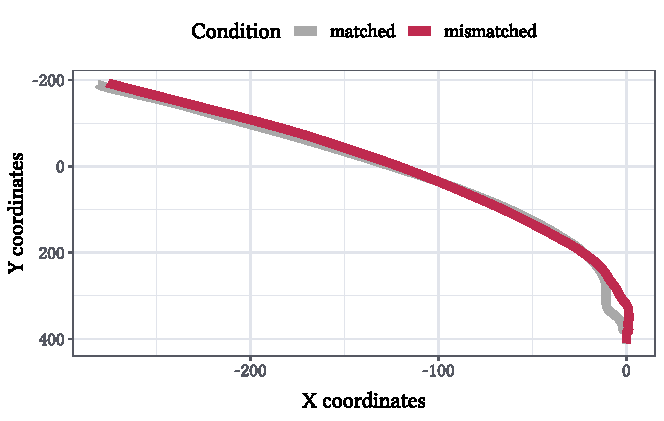
\includegraphics[]{figures/fig7.8.pdf}
    \caption{Mean trajectories of mouse-tracks for matched and mismatched item trials.}
    \label{fig:7_8}
\end{figure}

Initially, regular Gaussian generalised additive mixed models were fitted to the X and Y coordinates of the mouse-track data. However, model criticism revealed that the fitted GAMMs showed rather problematic amounts of autocorrelation. Autocorrelation, or more specifically temporal spatial autocorrelation, is the association between data values over time. Depending on the sign of autocorrelation, model estimates can either be over- or underestimated (\cite{Charlton2009}). Thus, models with a high degree of autocorrelation are unreliable in their predictions. It was therefore decided to use QGAMs instead of GAMMs. QGAMs, as briefly introduced in Section \ref{section03_2_2}, are additive quantile regression models. They are a distribution-free method for estimating the predicted values for any given quantile of the response distribution. As QGAMs are a relatively new tool within the toolbox of GAMs, I will explain the main characteristics of QGAMs as introduced by \citet{Fasiolo2021} in the following. The interested reader is referred to the aforementioned paper for a more thorough mathematical introduction. 

Quantile regression, as conducted by QGAMs, aims at modelling the $\tau$th quantile of the response, $y$, conditionally on a $p$-dimensional vector of covariates, $x$, with $k$ basis functions, where $\tau \in (0,1)$. The $\tau$th quantile then is 

\begin{equation}
\label{eq:mu}
    \mu=\inf \left \{ y:F(y|x)\geq \tau \right \}.
\end{equation}

This can also be defined as the minimiser of the expected loss

\begin{equation}
\label{eq:Lmux}
    L(\mu|x)=\int \rho_{\tau}(y-\mu)dF(y|x),
\end{equation}

\noindent where the quantity $\rho_{\tau}(z)$ is the pinball loss (\cite{Koenker2005, Gneiting2011}), which attributes different weights to observations depending on the sign of the residuals $z$:

\begin{equation}
\label{eq:rhotauz}
    \rho_{\tau}(z)=\left \{ \begin{matrix}
    (\tau+1)z\ & \mathrm{if}\, z<0\\ 
    \tau z & \mathrm{if} \, z\geq 0
    \end{matrix} \right..
\end{equation}

The quantile estimator is thus penalised to prevent overfitting, and the amount of penalisation is determined by the so-called learning rate, which determines the relative weight of the loss and the penalty. A QGAM then is defined as

\begin{equation}
\label{eq:mutaui}
    \mu_{\tau}(i)=\beta_{0}+\sum_{k=1}^{\rho}f_{k}(x_{i,k})+b_{\ell_{i}}.
\end{equation}

The term $\sum_{k=1}^{\rho}f_{k}(x_{i,k})$ can represent either a linear effect or a non-linear effect without a predefined structure. $b_{\ell_{i}}$ models random intercepts for group $\ell=1,...,L$ to which observation $i$ belongs, and $\beta_{0}$ is the y-intercept.

In less technical terms, QGAMs make use of the general features of GAMs in modelling linear and non-linear effects as well as random effects. Instead of taking into account the whole range of data for their fitting process, each QGAM is restricted to a given conditional quantile of the data. Splitting the data into ten equally sized conditional quantiles, one can infer, for example, the following. Let us assume that the data are ordered from lowest to highest value, as is the case for the density plots of Figure \ref{fig:7_9} Then the so-called $0.1$ quantile (Panel A) will consist of the first 10\% of data, that is the tenth of the data consisting of the lowest values. The $0.5$ quantile (Panel B), then, consists of the first 50\% of the data, and the $0.9$ quantile (Panel C) contains all data but the highest 10\%. 

\begin{figure}
    \centering
    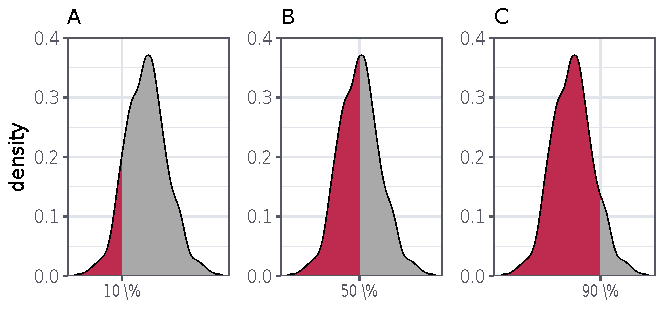
\includegraphics[width=0.9\textwidth]{figures/fig7.9.pdf}
    \caption{Illustration of the three conditional quantiles $0.1$ (Panel A), $0.5$ (Panel B), and $0.9$ (Panel C) in blue.}
    \label{fig:7_9}
\end{figure}

Fitting QGAMs to several of these quantiles allows for a detailed picture of the effects to be investigated. If an effect is present in the $0.1$ quantile but no longer present in the $0.3$ quantile, for example, one can conclude that the effect is significant for data of the lowest 10\% but loses its significance when taking into account higher valued data points. If the same effect then regains its significance in the $0.5$ quantile, one can conclude the opposite. While there is no effect for the lowest 30\% of data points, there again is an effect when including the following 20\% of data points. QGAMs take into account all covariates specified in their model formula to arrive at their weighted conditional quantile distribution. 

Before one can model X and Y coordinates of mouse-tracks as provided by the \texttt{mousetrap} plugin (\cite{Kieslich2017}) for OpenSesame, the data have to be prepared. After the initial preparations mentioned at the beginning of this section, i.e. after time-normalisation and spatial transformation, the \texttt{mousetrap} package (\cite{Kieslich2019}) provides coordinates and other data in R in a so-called mousetrap object. To extract the pertinent data needed, i.e. the X and Y coordinates, the time stamps corresponding to each coordinate value, as well as a unique identifier per trial, the \texttt{extract\_x}, \texttt{extract\_y}, and \texttt{extract\_t} functions of the \texttt{mtqgam} package (\cite{Schmitz2021mtqgam}) were used. 

Taking a closer look at the extracted coordinate data, it is found that the coordinate system as used per default by the \texttt{mousetrap} plugin (see, for example, axes in Figure \ref{fig:7_7} and Figure \ref{fig:7_8}) is rather unintuitive for the Y dimension: Coordinates higher up on the screen show negative Y coordinate values, while coordinates lower down on the screen show positive Y coordinate values. For X coordinates, the system is more intuitive: Coordinates further to the right have positive X coordinate values, while coordinates further to the left have negative X coordinate values. Using this default coordinate system would result in an obscure order of conditional quantiles. Consider the $0.1$ conditional quantile, which consists of the lowest 10\% of data points, as an example. As Y shows lowest values for mouse positions high up on the screen and X shows lowest values for mouse positions further to the left, the first quantile would correspond to the end or near-end of the mouse-tracks instead of to their start. Analogously, the $0.9$ quantile, then, would correspond to the start or near-start of the mouse-tracks. Thus, modelling the coordinate data with their default sign means doing things from back to front. For this reason, the original coordinate data’s sign was reversed.

Merging the coordinate and time stamp data with the data on the set of covariates provided in Section \ref{section07_2_1}, one can then model QGAMs. As mentioned previously, the coordinates used in the present analysis are time-normalised. For the current implementation, I chose a number of n = 140 time steps for the time-normalisation process. \citet{Kieslich2019} provide no reasoning on why the \texttt{mousetrap} package uses a number of n = 101 per default but refer to \citet{Spivey2005} instead. However, in \citet{Spivey2005} the number of time steps remains unmotivated. I arrived at n = 140 by arbitrarily taking the mean RT of all trials $\bar{x}\approx 1400$ ms and dividing it by $10$. An example of the prepared data is given in Table \ref{tab:7.8}.

\begin{table}\fontsize{9}{10}
\caption{Example of the data format for a matched trial.}
\label{tab:7.8}
\centering
\begin{tabular}{rrrrrr} 
\lsptoprule
\textsc{order} & \textsc{trialNumber} & \textsc{time}      & \textsc{x\_coordinate} & \textsc{y\_coordinate} & \textsc{condition}  \\ 
\midrule
1     & 1           & 0         & 0             & -380.000      & matched    \\
…     & …           & …         & …             & …             & …          \\
66    & 1           & 585.4700  & -2.000        & -380.000      & matched    \\
67    & 1           & 594.4748  & -2.000        & -380.000      & matched    \\
68    & 1           & 603.4800  & -2.348        & -382.652      & matched    \\
…     & …           & …         & …             & …             & …          \\
110   & 1           & 972.7770  & 113.944       & -124.724      & matched    \\
111   & 1           & 981.7840  & 121.141       & -103.685      & matched    \\
…     & …           & …         & …             & …             & …          \\
130   & 1           & 1152.9210 & 238.000       & 216.000       & matched    \\
131   & 1           & 1233.9860 & 238.000       & 216.000       & matched    \\
\lspbottomrule
\end{tabular}
\end{table}

For each \textsc{trialNumber} the prepared data set contains a separate row for each time step. The individual time steps are numbered in the variable \textsc{order}. The point in time of the time stamp is given in \textsc{time}. For each time stamp, the X and Y coordinates are contained in \textsc{x\_coordinate} and \textsc{y\_coordinate}, respectively. \textsc{condition}, then, is the previously introduced explanatory variable of interest, and its value is repeated for each row of a trial. The same is true for all other covariates of the data set (not shown in Table \ref{tab:7.8}). In the above example, the first row is the very first coordinate pair recorded at time $0$. The data of rows 66 to 68 show that even though time passed, the mouse was not moved at all (rows 66 to 67) or moved only slightly (rows 67 to 68). From rows 110 to 111, mouse movement is clearly visible in the X and Y coordinates. Finally, in rows 130 and 131 (and following), the target is reached. Thus, time continues to pass until time stamp number 140 is reached, while X and Y coordinates remain unchanged.

\subsubsection{Fitted models}\label{section07_2_3_1}

The complete set of data (n = 261,240) was split into two separate data sets depending on whether the (pseudo-)base of the target word belonged to a singular or plural noun. This resulted in two smaller data sets, with n = 142,380 for singular pseudo-bases and n = 118,860 for plural bases. This was done because the aim of the present analysis was to investigate whether a mismatch of (pseudo-)base and /s/ duration influenced the mouse-tracks. While this can also be found out with the complete data set, interactions of (pseudo-)base types and further covariates would have been a necessary part of the model formula. It was decided against using such multiple interactions as they make model interpretation more complex while offering basically the same insights as the implementation with split data sets. Moreover, fitting QGAMs is computationally costly, with near-exponentially increasing computation times for bigger data sets and more complex effect structures. Thus, choosing the implementation of several QGAMs for smaller data sets also kept the carbon footprint of the analysis down.

Both data sets were then further reduced by excluding trials which had been responded to incorrectly. While \textsc{correct} was a potential covariate for modelling QGAMs, the difference between correctly and incorrectly answered trials is not the main interest of the present study. This decision led to an overall loss of n = 46,760 data points (17.9\%), resulting in n = 102,480 for singular pseudo-bases and n = 112,000 for plural bases. An overview of all variables contained in the two data sets is given in Table \ref{tab:7.9} and Table \ref{tab:7.10}.

\begin{table}\fontsize{10}{11}
\caption{Summary of the dependent variables and the numerical and categorical predictors in the singular pseudo-base data set.}
\label{tab:7.9}
\centering
\begin{tabular}{lrrrr} 
\lsptoprule
Dependent variables    & Mean     & St. Dev.                  & Min      & Max                           \\ 
\midrule
\textsc{x\_coordinate}          & 74.643   & 152.998                   & -511.000 & 512.000                       \\
\textsc{y\_coordinate}          & -176.898 & 250.926                   & -410.000 & 384.000                       \\ 
\midrule
Numerical predictors   & Mean     & St. Dev.                  & Min      & Max                           \\ 
\midrule
\textsc{order}                  & 70.500   & 40.414                    & 1.000    & 140.000                       \\ 
\midrule
Categorical predictors & \multicolumn{1}{l}{Levels}   & ~                         & ~        & ~                             \\ 
\midrule
\textsc{item}                   & \multicolumn{1}{l}{12}       & ~                         & ~        & ~                             \\
\textsc{subject}                & \multicolumn{1}{l}{39}       & ~                         & ~        & ~                             \\ 
\midrule
Explanatory variable   & \multicolumn{1}{l}{Levels}   & ~                         & ~        & ~                             \\ 
\midrule
\textsc{condition}              & \multicolumn{2}{l}{\texttt{matched}:
  50120} & \multicolumn{2}{l}{\texttt{mismatched}:
  52360}  \\
\lspbottomrule
\end{tabular}
\end{table}





\begin{table}\fontsize{10}{11}
\caption{Summary of the dependent variables and the numerical and categorical predictors in the plural base data set.}
\label{tab:7.10}
\centering
\begin{tabular}{lrrrr} 
\lsptoprule
Dependent variables    & Mean     & St. Dev.                  & Min      & Max                           \\ 
\midrule
x\_coordinate          & 75.413   & 150.252                   & -512.000 & 511.000                       \\
y\_coordinate          & -192.441 & 243.169                   & -410.000 & 384.000                       \\ 
\midrule
Numerical predictors   & Mean     & St. Dev.                  & Min      & Max                           \\ 
\midrule
order                  & 70.500   & 40.414                    & 1.000    & 140.000                       \\ 
\midrule
Categorical predictors & \multicolumn{1}{l}{Levels}   & ~                         & ~        & ~                             \\ 
\midrule
\textsc{item}                   & \multicolumn{1}{l}{12}       & ~                         & ~        & ~                             \\
\textsc{subject}                & \multicolumn{1}{l}{39}       & ~                         & ~        & ~                             \\ 
\midrule
Explanatory variable   & \multicolumn{1}{l}{Levels}   & ~                         & ~        & ~                             \\ 
\midrule
\textsc{condition}              & \multicolumn{2}{l}{\texttt{matched}:
  50120} & \multicolumn{2}{l}{\texttt{mismatched}:
  52360}  \\
\lspbottomrule
\end{tabular}
\end{table}

For both data sets, two sets of QGAMs were fitted. One set of QGAMs was fitted to X coordinates, and one set of QGAMs was fitted to Y coordinates. I aimed at estimating the conditional quantiles corresponding to $\tau=0.1,0.3,0.5,0.7$ and $0.9$. Thus, each set of QGAMs consisted of five QGAMs, one for each of the five quantiles. Taking into account more extreme quantiles, i.e. $0.1$ and $0.9$, as well as the median quantile $0.5$ and the quantiles between the median and the extreme quantiles, i.e. $0.3$ and $0.7$, one obtains a detailed picture of how predictors affect the coordinate data. In total, ten QGAMs for each of the two data sets were fitted, that is five for X coordinates and five for Y coordinates. This resulted in a total number of twenty QGAMs.

The model formula for all QGAMs was similar. The dependent variable was either \textsc{x\_coordinate} or \textsc{y\_coordinate}. \textsc{condition} was introduced as parametric term. \textsc{order} was given as smooth term with the default \textit{k}-value of $9$, and \textsc{item} and \textsc{subject} were included as random smooth terms. The model formula was kept simple due to the extensive computational times of QGAMs. 

All models were then checked according to the process introduced in Section \ref{section03_2_2}. It was found that the \textit{k}-index value of the \textsc{order} smooth term was well below $0.05$ for all QGAMs, thus indicating potentially missed patterns. Re-modelling the set of QGAMs for X coordinates of plural bases as a test case with higher \textit{k}-values ($k=18,30,60$, and $120$) revealed that no matter what the \textit{k}-value, the general effect of all covariates remained unchanged. Following \citet{Wood2017}, it was therefore concluded that the \textit{k}-value was large enough so that re-fitting all twenty computationally costly QGAMs was not necessary. The final data sets, as well as the analysis and results discussed in the following sections, can be found in the supplementary material given in Chapter \ref{Supplementary Material}.

\subsubsection{Results}\label{section07_2_3_2}

Across all twenty models, an effect of \textsc{condition} was found 12 times. An effect of the \textsc{order} smooth was found in all models. Similarly, the random smooths of \textsc{item} and \textsc{subject} reached significance in all QGAMs. The overall model fit is high with a mean deviance explained of $\overline{D}=70.74$\%. For both data sets, QGAMs fitted to Y coordinates show overall higher rates of deviance explained ($\overline{D}=79.67$\%) than their X coordinate counterparts ($\overline{D}=61.81$\%). For all four sets of QGAMs, the QGAM fitted to the $0.5$ quantile shows the lowest rate of deviance explained ($\overline{D}_{0.5}=61.15$\%), while the QGAMs fitted to the more extreme quantiles show the highest rates of deviance explained ($\overline{D}_{0.1}=82.86$\% and $\overline{D}_{0.9}=79.63$\%).

The effects found in the QGAMs fitted to X and Y coordinates of the monomorphemic pseudo-base data set are displayed in Table \ref{tab:7.11}. The model estimates of these and all following QGAMs are part of the supplementary material given in Chapter \ref{Supplementary Material}. Note that here and in the following, I will refrain from discussing the effects of the smooth terms as they are not the main interest of investigation. 

There are significant effects of \textsc{condition} in four QGAMs fitted to the X coordinate data and in four QGAMs fitted to Y coordinate data. For $\tau=0.3,0.5,0.7$ and $0.9$ \textsc{condition} shows a significant effect for X and Y coordinates. The effects are illustrated in Figure \ref{fig:7_10}. Where a significant effect is found, X coordinates are further to the right and Y coordinates are further down in the mismatched \textsc{condition}. Recall that QGAMs rely on conditional quantiles. Thus, the estimates shown in Figure \ref{fig:7_10} and similar plots illustrate the nature of an effect taking into account a certain quantity of the overall data (e.g. the lowest 10\% of dependent variable data values in $\tau=0.1$). The estimates do not illustrate the positions of mouse-tracks at certain points of their trajectory.

\begin{table}\fontsize{9}{10}
\caption{Summary of the effects found in the QGAMs fitted to the X and Y coordinates of the monomorphemic pseudo-base data set. Significance codes: *** $p < 0.001$, ** $p < 0.01$, * $p < 0.05$.}
\label{tab:7.11}
\centering
\begin{tabular}{lrrrrrrrrrrr}
\lsptoprule
~                   & \multicolumn{5}{c}{X coordinates}       & \multicolumn{1}{c}{}                       & \multicolumn{5}{c}{Y coordinates}                               \\
\midrule
\multicolumn{1}{r}{quantiles:}          & 0.1        & 0.3        & 0.5        & 0.7        & 0.9 & ~        & 0.1        & 0.3        & 0.5        & 0.7        & 0.9         \\
\midrule
Parametric Terms    & \textbf{~} & \textbf{~} & \textbf{~} & \textbf{~} & \textbf{~} & \textbf{~} & \textbf{~} & \textbf{~} & \textbf{~} & \textbf{~}  \\
\midrule
(Intercept)         & ***        & ***        & ***        & ***        & *** & ~       & ***        & ***        & ***        & ***        & **          \\
\textsc{condition}\texttt{mismatched} & n.s.       & *          & ***        & ***        & ***   & ~     & n.s.       & ***        & ***        & ***        & ***         \\
\midrule
Smooth Terms        & \textbf{~} & \textbf{~} & \textbf{~} & \textbf{~} & \textbf{~} & \textbf{~} & \textbf{~} & \textbf{~} & \textbf{~} & \textbf{~}  \\
\midrule
\textsc{order}               & ***        & ***        & ***        & ***        & ***  & ~      & ***        & ***        & ***        & ***        & ***         \\
\midrule
Random Smooth Terms & \textbf{~} & \textbf{~} & \textbf{~} & \textbf{~} & \textbf{~} & \textbf{~} & \textbf{~} & \textbf{~} & \textbf{~} & \textbf{~}  \\
\midrule
\textsc{item}                & ***        & ***        & ***        & ***        & ***   & ~     & ***        & ***        & ***        & ***        & ***         \\
\textsc{subject}             & ***        & ***        & ***        & ***        & ***   & ~     & ***        & ***        & ***        & ***        & ***        \\
\lspbottomrule
\end{tabular}
\end{table}

\begin{figure}
    \centering
    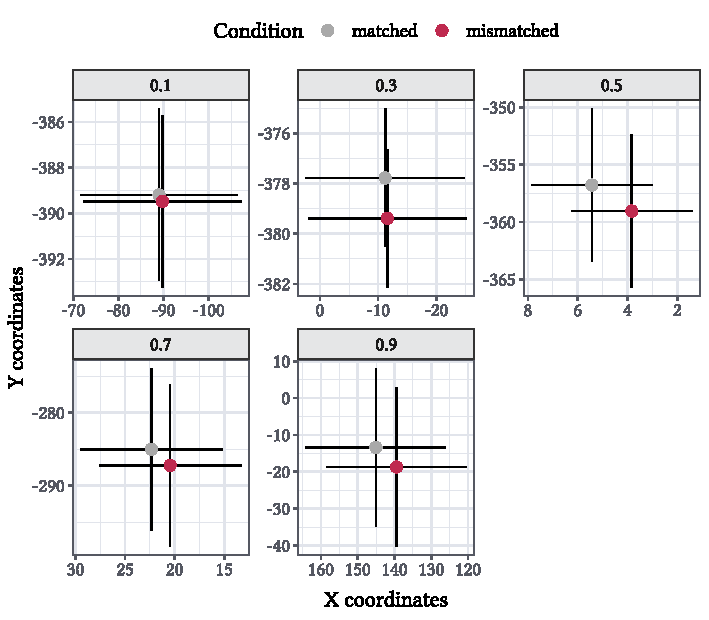
\includegraphics[]{figures/fig7.10.pdf}
    \caption{Effects of \textsc{condition} as found in the QGAMs modelled to the X and Y coordinates of the monomorphemic pseudo-base data set. The lines indicate the confidence intervals of the estimated X and Y coordinate values.}
    \label{fig:7_10}
\end{figure}

For the QGAMs fitted to the plural base data set, the effects found for X and Y coordinates are given in Table \ref{tab:7.12}. \textsc{condition} reaches significance in four models fitted to the X coordinate data: $\tau=0.1,0.3,0.5$ and $0.7$. The effect is illustrated in Figure \ref{fig:7_11}. Where \textsc{condition} shows a significant effect for X coordinates, coordinates of mismatched trials are further to the right. For Y coordinates, \textsc{condition} misses significance across all models.

\begin{table}\fontsize{9}{10}
\caption{Summary of the effects found in the QGAMs fitted to the X and Y coordinates of the plural base data set. Significance codes: *** $p < 0.001$, ** $p < 0.01$, * $p < 0.05$.}
\label{tab:7.12}
\centering
\begin{tabular}{lrrrrrrrrrrr}
\lsptoprule
~                   & \multicolumn{5}{c}{X coordinates}       & \multicolumn{1}{c}{}                        & \multicolumn{5}{c}{Y coordinates}                               \\
\midrule
\multicolumn{1}{r}{quantiles:}          & 0.1        & 0.3        & 0.5        & 0.7        & 0.9  & ~       & 0.1        & 0.3        & 0.5        & 0.7        & 0.9         \\
\midrule
Parametric Terms    & \textbf{~} & \textbf{~} & \textbf{~} & \textbf{~} & \textbf{~} & \textbf{~} & \textbf{~} & \textbf{~} & \textbf{~} & \textbf{~}  \\
\midrule
(Intercept)         & **        & ***        & ***        & ***        & *** & ~       & ***        & ***        & ***        & ***        & ***          \\
\textsc{condition}\texttt{mismatched} & **       & ***          & ***        & **        & n.s.  & ~      & n.s.       & n.s.        & n.s.        & n.s.        & n.s.         \\
\midrule
Smooth Terms        & \textbf{~} & \textbf{~} & \textbf{~} & \textbf{~} & \textbf{~} & \textbf{~} & \textbf{~} & \textbf{~} & \textbf{~} & \textbf{~}  \\
\midrule
\textsc{order}               & ***        & ***        & ***        & ***        & *** & ~       & ***        & ***        & ***        & ***        & ***         \\
\midrule
Random Smooth Terms & \textbf{~} & \textbf{~} & \textbf{~} & \textbf{~} & \textbf{~} & \textbf{~} & \textbf{~} & \textbf{~} & \textbf{~} & \textbf{~}  \\
\midrule
\textsc{item}                & ***        & ***        & ***        & ***        & ***  & ~      & ***        & ***        & ***        & ***        & ***         \\
\textsc{subject}             & ***        & ***        & ***        & ***        & ***  & ~      & ***        & ***        & ***        & ***        & ***        \\
\lspbottomrule
\end{tabular}
\end{table}

\begin{figure}
    \centering
    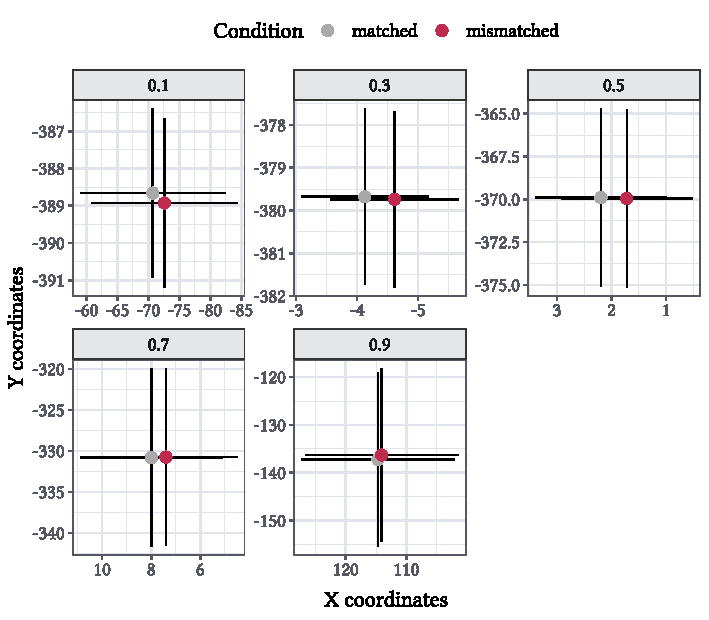
\includegraphics[]{figures/fig7.11.pdf}
    \caption{Effects of \textsc{condition} as found in the QGAMs modelled to the X and Y coordinates of the plural base data set. The lines indicate the confidence intervals of the estimated X and Y coordinate values.}
    \label{fig:7_11}
\end{figure}

\subsubsection{Interim summary: Mouse-tracks}\label{section07_2_3_3}

Across all QGAMs, a significant effect of \textsc{condition} emerged 12 times. Especially X coordinates are affected by \textsc{condition}, as 8 of the 12 significant effects are found in QGAMs fitted to X coordinate data. For Y coordinates, significant effects of \textsc{condition} are only found in the monomorphemic pseudo-base data set. Where a significant effect is found, coordinates of mismatched trials are further to the right and lower down.

\section{Discussion}\label{section07_3}

The present number-decision study set out to investigate if listeners make use of subphonemic durational differences in the comprehension of non-morphemic and plural word-final /s/. This question was analysed following \textsc{H comp}, the \textit{Mismatch Hypothesis}: If subphonemic durational differences are made use of, then a mismatch of subphonemic detail and intended meaning leads to a) slowed down comprehension processes and b) deviated mouse trajectories.

Part a) of the hypothesis was tested by modelling the reaction time data in a PAMM. It was found that reaction times are not significantly influenced by the mismatch of durational information. As such, the first part of the hypothesis is rejected. That is, reaction times are similar for trials with matched and mismatched durational information. Thus, comprehension processes apparently are not slowed down.

Part b) of the hypothesis was investigated by fitting QGAMs to the X and Y coordinate data of the mouse-tracks recorded during the experiment. QGAMs were fitted separately for singular pseudo-bases and plural bases to achieve a way of direct comparisons between matched and mismatched /s/ trials within one type of (pseudo-)base. The results of the QGAMs show an overall significant effect of matched versus mismatched durational information on X coordinates. That is, X coordinates of trials with durationally mismatched items are significantly further to the right. For Y coordinates, significant effects were only found in the singular pseudo-base data: Mismatched trials come with Y coordinates which are further down. 

How do these findings relate to the second part of the hypothesis? Looking at the results for X coordinates, which are further to the right in mismatched trials, one can interpret the findings as a confirmation of the hypothesis. Recall that mouse-tracks were mirrored where applicable, that is all tracks move towards the upper left corner of the coordinate system. Thus, an ideal non-deviated trajectory would be a straight line between the mouse cursor starting position and one of the answer options. As this non-deviated straight line moves linearly towards the upper left corner, X coordinates which are further to the right can be understood as deviation from that direct path and as a detour towards the other answer. Taking into account that the X coordinates of mismatched trials are overall significantly further to the right, then, one can conclude that mismatched durational information led to overall higher deviations from the direct path. While this effect on X coordinates was found for both data sets, the effect on Y coordinates was only found for singular pseudo-bases. Analogously, the lower Y coordinates for mismatched trials can be interpreted as a deviation from the direct path. Thus, the results of the mouse-tracking analysis confirm the second part of the hypothesis: Mouse-tracks of trials with mismatched items are deviated.

However, there are two major points that need to be addressed. First, the analysis did not consider whether the word-final /s/ of a particular stimulus has been heard already. While this, in theory, should not pose a problem, because QGAMs were fitted to quantiles across the distribution of coordinates and thus included ranges of coordinates for which the word-final /s/ has been heard, I nonetheless checked whether a difference in results is found. For this, I created two binary variables: \textsc{s\_onset} and \textsc{s\_offset}. \textsc{s\_onset} encodes the time of the onset of the word-final /s/ and \textsc{s\_offset} encodes the time of the offset of the word-final /s/. Based on these variables, I created data sets which contained only data for which either the onset of the /s/ was audible or for which the offset of the /s/ was audible already. Using these data sets, I refitted the QGAMs presented in the main analysis of this chapter. The overall results of these new QGAMs are similar to those reported here (see the supplementary material given in Chapter \ref{Supplementary Material}). Thus, considering only data for which the onset or offset of the word-final /s/ was audible does not change the general results.

Second, the analysis presented in this chapter excluded time as a relevant factor. Recall that all mouse-tracks were time-normalised during the pre-processing of the data. While this made mouse-tracks more easily comparable for my purposes, time is nonetheless a factor one might consider in other types of analyses. Following, for example, \citet{Blazej2015}, one can analyse the raw, non-normalised mouse trajectories. For this, I divided all X and Y coordinate data into 200 increments of 10 ms. The average for all of these increments was then calculated. The result of this procedure is illustrated in Figure \ref{fig:7_12}. As indicated by the dashed line, the /s/ onset was on average at 389 ms, while the /s/ offset, as indicated by the dotted line, was at 689 ms after the stimulus onset. Comparing Panels A and B, higher deviations between coordinates of matched and mismatched stimuli are again found for X coordinates as compared to Y coordinates. For both types of coordinates, differences between the trajectories become visible between the onset and offset of the word-final /s/. This finding indicates that listeners make use of the durational information. As time unfolds, the duration of the pertinent /s/ either corresponds to its expected duration (match) or it over-/undershoots its expected duration (mismatch). In the latter case, then, this mismatch of expected and perceived duration leads to a deviation of the mouse-track towards the other option. Considering time as a factor thus confirms the main findings of this chapter and provides further insight into the found effects.

\begin{figure}[t]
    \centering
    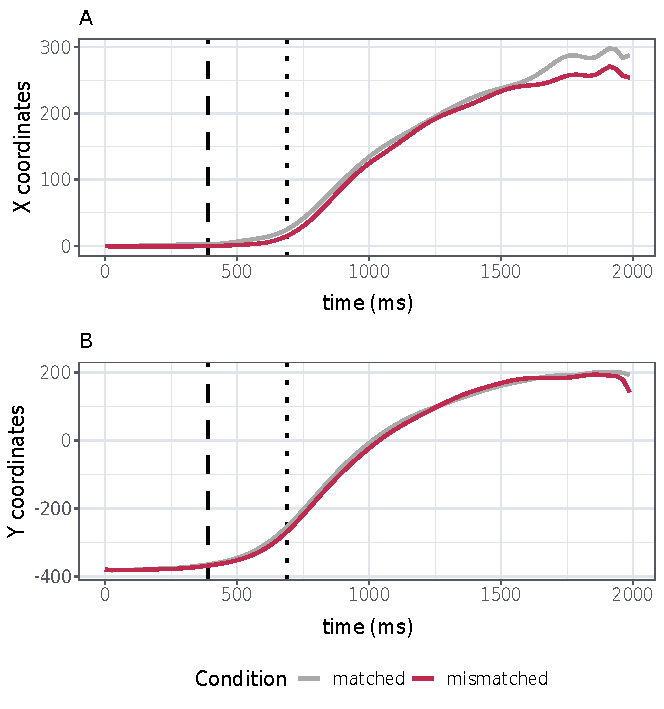
\includegraphics[width=0.9\textwidth]{figures/fig7.12.pdf}
    \caption{Averaged mouse position on the x-axis (Panel A) and on the y-axis (Panel B) for matched and mismatched trials as a function of time. The dashed horizontal lines indicate the average /s/ onset time; the dotted horizontal lines indicate the average /s/ offset time.}
    \label{fig:7_12}
\end{figure}

Let us now turn to the theoretical implications of the present results. As participants of the present study showed an influence of subphonemic durational differences on their comprehension in terms of mouse-tracks, theories which exclude such information from the result of the perception process cannot account for these findings (e.g. \cite{Klatt1979, McClelland1986, Norris1994, Norris2008}). If perception as such is not sensitive to subphonemic durational differences, and as a result, no such information is forwarded to the comprehension process, the comprehension process cannot make use of such durational detail. Thus, no difference between matched and mismatched trials should have been found. However, such theories can account for the null results of the reaction time analysis.

Exemplar and hybrid models (e.g. \cite{Goldinger1996, Hawkins2001, Pierrehumbert2002, Hanique2013Aalders}) as well as computational models such as DIANA (\cite{tenBosch2015, tenBosch2021}) and LDL (\cite{Baayen2019}) can potentially account for the findings of the mouse-track analysis. As such approaches assume the storage of fine-phonetic detail, such detail can be perceived and made use of in comprehension. However, it remains unclear why an effect of subphonemic durational information is found in mouse-tracks but not in reaction times.

Overall, it seems that no theoretical account can straightforwardly explain the findings of the present number-decision task. While reaction times are not influenced by durational mismatches in word-final /s/, mouse-tracks are. One might argue that reaction times on the one hand and mouse-tracks on the other hand represent different parts of the comprehension process, deliver different amounts of detail on the comprehension process, or show different levels of sensitivity towards mismatched information. Reaction times provide a single data point per trial and allow for little insight into the time window between the start and end of a trial. Even when analysed with novel sophisticated statistical methods such as PAMMs, they provide much less detail on what happens during a particular trial as compared to the continuously measured mouse-tracks. Thus, reaction times between matched and mismatched trials may very well be similar as is the case in the present study, while what happens before a response is recorded is not. These potential differences in the time window between the start of the trial and the response are captured by mouse-tracks. In the present case, this more detailed account of the comprehension process showed a significant influence of mismatched durational information. The present findings, then, can be understood as non-contradictory, as their underlying measures, reaction times and mouse-tracks, capture different aspects of the comprehension process: speed versus decision-making.

However, a detailed account of such potential differences is a subject for future research. Similarly, it has been briefly shown that time should not be disregarded for the analysis of mouse-tracking data. Thus, further analyses considering time as a factor, for example, an analysis of saccades, should be the aim of future research. Finally, one question remains: Are the results presented in this chapter confounded by lexical effects of the real word items used as stimuli? To investigate this question, a second comprehension task in which pseudowords were used is presented in the following chapter.

%\chapter{Comprehension of plural and clitic /s/}\label{chapter08}

As explained in detail in Section \ref{section02_2}, two comprehension studies are part of this book. This chapter presents the second of these studies on the comprehension of subphonemic differences in word-final /s/. The two studies differ in two main regards. First, the comprehension study described in Chapter \ref{chapter07} made use of real words in isolation, the comprehension study presented in this chapter uses pseudowords embedded within sentences as stimuli. Second, the first comprehension study used non-morphemic and plural word-final /s/, while this second study uses plural, \textit{is}-, and \textit{has}-clitic word-final /s/. As in the previous comprehension study, effects on comprehension were tested using a number-decision task in a mouse-tracking paradigm. Considering extant models and approaches of speech perception and comprehension, \textsc{H comp}, the \textit{Mismatch Hypothesis}, again is explored. However, taking into account the findings of the first comprehension study, reaction times are not investigated in the present study. That is, only the second part of the hypothesis is considered: If listeners make use of subphonemic durational differences in the comprehension of different types of word-final /s/, then a mismatch of subphonemic detail and intended meaning is expected to lead to deviated mouse trajectories.

\section{Methdology}\label{section08_1}

\subsection{Participants}\label{section08_1_1}

Forty-two native speakers of New Zealand English took part in the experiment. Their mean age was 22.5 years, ranging from 18 to 54. Eight participants identified as multilingual. The experiment took place at the University of Canterbury, Christchurch, New Zealand, from December 2020 to March 2021.

\subsection{Materials}\label{section08_1_2}

The speech materials consisted of pseudowords embedded within sentences. The pseudowords used are those forty-eight described in Section \ref{section03_1_2}. I repeat all pseudowords in Table \ref{tab:8.1} for convenience.

\begin{table}\fontsize{10}{11}
\caption{Orthographic (\textit{orth.}) and phonological (\textit{phon.}) representations of all pseudowords used in the number-decision task.}
\label{tab:8.1}
\centering
\begin{tabular}{lcccccc} 
\lsptoprule
~              & /glɪ/          & /prʌ/          & /pli:/          & /clu:/          & /blaʊ/          & /gleɪ/           \\ 
\midrule
\textit{orth.} & \textit{glips} & \textit{prups} & \textit{pleeps} & \textit{cloops} & \textit{bloups} & \textit{glaips}  \\
\textit{phon.} & /glɪps/        & /prʌps/        & /pli:ps/        & /klu:ps/        & /blaʊps/        & /gleɪps/         \\ 
\midrule
\textit{orth.} & \textit{glits} & \textit{pruts} & \textit{pleets} & \textit{cloots} & \textit{blouts} & \textit{glaits}  \\
\textit{phon.} & /glɪts/        & /prʌts/        & /pli:ts/        & /klu:ts/        & /blaʊts/        & /gleɪts/         \\ 
\midrule
\textit{orth.} & \textit{gliks} & \textit{pruks} & \textit{pleeks} & \textit{clooks} & \textit{blouks} & \textit{glaiks}  \\
\textit{phon.} & /glɪks/        & /prʌks/        & /pli:ks/        & /klu:ks/        & /blaʊks/        & /gleɪks/         \\ 
\midrule
\textit{orth.} & \textit{glifs} & \textit{prufs} & \textit{pleefs} & \textit{cloofs} & \textit{bloufs} & \textit{glaifs}  \\
\textit{phon.} & /glɪfs/        & /prʌfs/        & /pli:fs/        & /klu:fs/        & /blaʊfs/        & /gleɪfs/         \\
\lspbottomrule
\end{tabular}
\end{table}

All pseudowords were embedded into short context sentences of either simple past, present progressive, or present perfect tense. Additionally, the remaining context disambiguated between plural and non-plural contexts. In sentences with simple past tense, the agents were two aliens of the same kind (see \ref{ex:8.1a:sentence8.1a} \& \ref{ex:8.1b:sentence8.1b}) doing something together or to each other. This ensured a plural reading of the context. In sentences with present progressive tense, agents were a single alien doing something to or with another alien in object position (see \ref{ex:8.2a:sentence8.2a} \& \ref{ex:8.2b:sentence8.2b}). In sentences with present perfect tense, agents were single aliens who had done something to or with another alien in object position (see \ref{ex:8.3a:sentence8.3a} \& \ref{ex:8.3b:sentence8.3b}). That is, for the \textit{is}- and \textit{has}-clitic, the following verb ensured the pertinent clitic reading of the context. Almost exclusively irregular verbs were used to create the context sentences to ensure no ambiguities between them. Twenty-four contexts per type of /s/ were created, resulting in a total number of seventy-two context sentences. See the supplementary material given in Chapter \ref{Supplementary Material} for a list of all verbs and contexts.

\ex.
\label{ex:8.1a:sentence8.1a}
	The \textit{glips} ate their lunch together.
	
\ex.
\label{ex:8.1b:sentence8.1b}
	The \textit{glips} blew a kiss to each other.

\ex.
\label{ex:8.2a:sentence8.2a}
	The \textit{glip’s} eating cake with the bloup. 

\ex.
\label{ex:8.2b:sentence8.2b}
	The \textit{glip’s} blowing a kiss to the bloup.
	
\ex.
\label{ex:8.3a:sentence8.3a}
    The \textit{glip’s} eaten the bloup’s lunch.
	
\ex.
\label{ex:8.3b:sentence8.3b}
	The \textit{glip’s} blown kisses to the bloup every day of their marriage.

The context sentences were made into a reading list, which was then read and recorded three times by a trained native speaker of New Zealand English. Recordings took place at the soundproof booth of the Department of Linguistics at the University of Tübingen. The recordings were sampled at 44.1 kHz, 16 bit.

For each sentence the best of the three recordings was chosen by manual inspection. First, all recordings were analysed using Praat following the segmentation conventions laid out in Section \ref{section04_1_4}. Recordings with production errors, e.g. laughter, stutter or vocal fry, or segmentation difficulties, e.g. the absence of a stop release, were dismissed. Second, the speaking rate of sentences was measured using a Praat script (\cite{deJong2008}) and then analysed in R. As the contexts used in the current experiment differ in length, i.e. in number of syllables, speaking rate appeared to be a more appropriate measurement of similarity across utterances as compared to duration itself as used in the previous two experiments. Speaking rate was computed as number of syllables divided by utterance duration. The resulting mean speaking rate was $3.024$ with a standard deviation of $0.551$. Lastly, for each sentence, the iteration closest to the mean speaking rate was chosen for further use in the experiment resulting in a final mean speaking rate of $3.021$ with a standard deviation of $0.380$.

Then, the final /s/ duration of all items was manipulated in such a way that it corresponded to the mean /s/ duration for plural, \textit{is}-, and \textit{has}-clitic /s/ found in the reference study by \citet{Plag2017}. That is, in the case of a plural context such as \ref{ex:8.1a:sentence8.1a} the duration of the final /s/ was changed to 283 ms, while in the case of \textit{is}-clitic contexts such as \ref{ex:8.2a:sentence8.2a} the duration of the final /s/ was changed to 261 ms, and in the case of \textit{has}-clitic contexts such as \ref{ex:8.3a:sentence8.3a} the duration of the final /s/ was changed to 253 ms. These versions are manipulated so that their /s/ durations match those of previous findings. Thus, these items are referred to as \textit{matched} items.

For \textit{mismatched} items, /s/ durations were changed as follows. For each plural context, two new versions were created. One contained the typical duration of an \textit{is}-clitic /s/, while the other one contained the typical duration of a \textit{has}-clitic /s/. For each \textit{is}-clitic and \textit{has}-clitic context, a new version was created with the duration of a typical plural /s/. The final number of contexts and their /s/ durations are given in Table \ref{tab:8.2}. Each participant took part in 192 trials, i.e. 2 × 24 matched plural /s/ items + 2 × 24 mismatched plural /s/ items + 24 matched \textit{is}-clitic /s/ items + 24 mismatched \textit{is}-clitic /s/ items + 24 matched \textit{has}-clitic /s/ items + 24 mismatched \textit{has}-clitic /s/ items.

\begin{table}\fontsize{9}{10}
\caption{Number of versions per type of word-final /s/ and their /s/ durations. Mean values are taken from \citet{Plag2017}.}
\label{tab:8.2}
\centering
\begin{tabular}{llll}
\lsptoprule
\textbf{~}                  & \begin{tabular}[c]{@{}l@{}}Version 1: \\matched\end{tabular}                   & \begin{tabular}[c]{@{}l@{}}Version 2: \\mismatched\end{tabular}               & \begin{tabular}[c]{@{}l@{}}Version 3: \\mismatched\end{tabular}                 \\
\midrule
\textit{is}-clitic context  & \begin{tabular}[c]{@{}l@{}}mean of \textit{is}-clitic /s/ \\261~ms\end{tabular}  & \begin{tabular}[c]{@{}l@{}}mean of plural /s/ \\283~ms\end{tabular}             & ~                                                                               \\
\midrule
\textit{has}-clitic context & \begin{tabular}[c]{@{}l@{}}mean of \textit{has}-clitic /s/ \\253~ms\end{tabular} & \begin{tabular}[c]{@{}l@{}}mean of plural /s/ \\283~ms\end{tabular}             & ~                                                                               \\
\midrule
plural context              & \begin{tabular}[c]{@{}l@{}}mean of plural /s/ \\283~ms\end{tabular}              & \begin{tabular}[c]{@{}l@{}}mean of \textit{is}-clitic /s/ \\261~ms\end{tabular} & \begin{tabular}[c]{@{}l@{}}mean of \textit{has}-clitic /s/ \\253~ms\end{tabular} \\
\lspbottomrule
\end{tabular}
\end{table}

\subsection{Procedure}\label{section08_1_3}

Similar to the experiment in Chapter \ref{chapter07}, the number-decision task was conducted in OpenSesame using the \texttt{mousetrap} plugin for mouse-tracking (\cite{Kieslich2017}). First, participants were introduced to the task at hand. They were told that in the following experiment they had to decide whether a sentence is about the action of two identical aliens, i.e. aliens of the same species and name, or about the action of one alien. They were told to mouse-click on the matching ``one" or ``two or more" button, respectively, in the top left and top right corner of the screen. Figure \ref{fig:8_1} illustrates what participants saw on screen for each trial. The participants were told that if they did not decide on either option within a certain amount of time, the next trial would start automatically. Each participant started with five practice trials.

\begin{figure}
    \centering
    \includegraphics[width=0.7\textwidth]{figures/fig8.1.png}
    \caption{Option display during the comprehension experiment. The mouse cursor indicates the position the mouse was reset to in each trial.}
    \label{fig:8_1}
\end{figure}

Each trial was preceded by a stretch of silence of 450 ms accompanied by a white screen. Then, one of the recordings was played, with reaction time and mouse-tracking measurement starting at the onset of the recording. Participants were given a window of 4500 ms starting after the onset of the recording to react, after that a time-out was recorded. The next trial then started automatically 5000 ms after the onset of the previous recording, starting with the next inter-trial white screen. Mouse-tracks were recorded with a frequency of 100 Hz.

\section{Analysis}\label{section08_2}

The analysis of the present data is similar to the analysis of the mouse-tracking data in the comprehension study on non-morphemic and plural word-final /s/ in Chapter \ref{chapter07}. First, mouse-tracking data were extracted, spatially transformed, and time-normalised with n = 140 time steps using the \texttt{mousetrap} package (\cite{Kieslich2019}) in R. Figure \ref{fig:8_2} shows the aggregated mean trajectory of the spatially transformed and time-normalised mouse-tracks in the lower left panel. The panel on top gives the overall distribution of all X coordinates, with a peak visible around a value of $0$. The panel on the right displays the overall distribution of all Y coordinates, with a peak around a value of $380$. As in Chapter \ref{chapter07}, the positions of the peaks corresponds to the position at which the mouse cursor started for each trial.

\begin{figure}
    \centering
    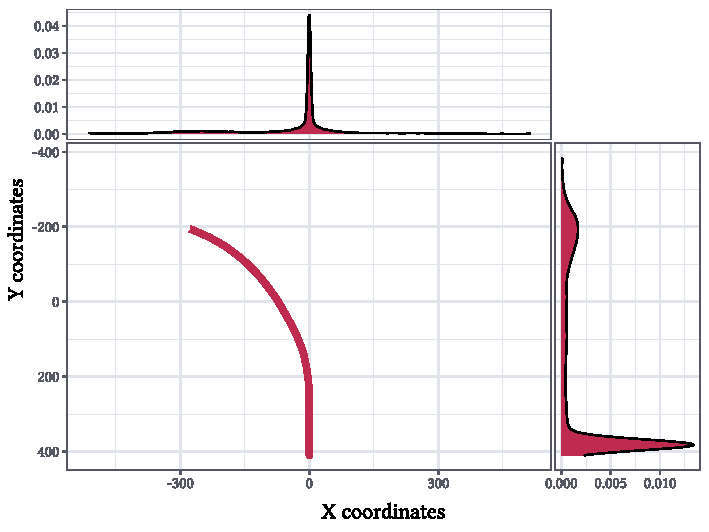
\includegraphics[]{figures/fig8.2.pdf}
    \caption{Mean trajectory of all spatially adjusted and time-normalised mouse-tracks (lower left), and density distribution of X and Y coordinates (on top and on the right, respectively).}
    \label{fig:8_2}
\end{figure}

Then, X and Y coordinates were extracted using the \texttt{mtqgam} package (\cite{Schmitz2021mtqgam}). As in Section \ref{section07_2_3}, the sign of the coordinate data were reversed to allow for a straightforward interpretation. An example of the resulting data structure is given in Table \ref{tab:8.3}.

\begin{table}\fontsize{9}{10}
\caption{Example of the data format for a matched trial.}
\label{tab:8.3}
\centering
\begin{tabular}{rrrrrr} 
\lsptoprule
\textsc{order} & \textsc{trialNumber} & \textsc{time}      & \textsc{x\_coordinate} & \textsc{y\_coordinate} & \textsc{condition}  \\ 
\midrule
1     & 1           & 0         & 0             & -380.000      & matched    \\
…     & …           & …         & …             & …             & …          \\
9     & 1           & 201.9568  & 2.000         & -380.000      & matched    \\
10    & 1           & 227.2014  & 3.440         & -379.560      & matched    \\
11    & 1           & 252.4460  & 6.734         & -375.266      & matched    \\
…     & …           & …         & …             & …             & …          \\
110   & 1           & 2751.6619 & 72.487        & 90.160        & matched    \\
111   & 1           & 2776.9065 & 139.647       & 120.597       & matched    \\
…     & …           & …         & …             & …             & …          \\
130   & 1           & 3256.5540 & 274.000       & 199.000       & matched    \\
131   & 1           & 3281.7986 & 274.000       & 199.000       & matched    \\
\lspbottomrule
\end{tabular}
\end{table}

Finally, the prepared data set was analysed using additive quantile regression models (QGAMs; \cite{Fasiolo2021}). 

\subsection{Fitted models}\label{section08_2_1}

The complete set of coordinate data (n = 1,017,800) was split into four separate data sets. Recall that there were three types of word-final /s/ involved in this study, i.e. plural, \textit{is}-, and \textit{has}-clitic /s/. Targets in plural context sentences were once manipulated to bear the mismatched /s/ duration of an \textit{is}-clitic, and once to bear the mismatched /s/ duration of a \textit{has}-clitic. An overview of the four subsets and the contexts they contain is given in Table \ref{tab:8.4}.

\begin{table}\fontsize{10}{11}
\caption{Overview of the four subsets used in the QGAM modelling process. Each subset contains mouse-track coordinate data of durationally matched and mismatched stimuli. Within each subset, the type of context is kept constant, while the manipulation of the pertinent word-final /s/ either corresponds to a match or mismatch in duration. Subset names contain information on the type of context (first subscript letter) and the /s/ duration that constitutes a mismatch (second subscript letter).}
\label{tab:8.4}
\centering
\begin{tabular}{llll} 
\lsptoprule
Subset name               & Condition  & Context             & /s/ duration           \\ 
\midrule
\multirow{2}{*}{\textsc{subset\textsubscript{IP}}} & matched    & \textit{is}-clitic  & \textit{is}-clitic   \\
                          & mismatched & \textit{is}-clitic  & plural               \\ 
\midrule
\multirow{2}{*}{\textsc{subset\textsubscript{HP}}} & matched    & \textit{has}-clitic & \textit{has}-clitic  \\
                          & mismatched & \textit{has}-clitic & plural               \\ 
\midrule
\multirow{2}{*}{\textsc{subset\textsubscript{PI}}} & matched    & plural              & plural               \\
                          & mismatched & plural              & \textit{is}-clitic   \\ 
\midrule
\multirow{2}{*}{\textsc{subset\textsubscript{PH}}} & matched    & plural              & plural               \\
                          & mismatched & plural              & \textit{has}-clitic  \\
\lspbottomrule
\end{tabular}
\end{table}

\textsc{subset\textsubscript{IP}} thus contained results on \textit{is}-clitic contexts with either \textit{is}-clitic /s/ or plural /s/ durations (n = 260,400). \textsc{subset\textsubscript{HP}} contained results on \textit{has}-clitic contexts with either \textit{has}-clitic /s/ or plural /s/ durations (n = 229,600). \textsc{subset\textsubscript{PI}} contained results on plural contexts with either plural /s/ or \textit{is}-clitic /s/ durations (n = 263,900). \textsc{subset\textsubscript{PH}}, finally, contained results on plural contexts with either plural /s/ or \textit{has}-clitic /s/ durations (n = 263,900). Similar to the analysis of mouse-tracks in the comprehension study on non-morphemic and plural /s/ presented in Section \ref{section07_2_3}, the individual subsets were created in order to determine whether a mismatch of context and word-final /s/ influenced mouse-tracks to a significant extent. While this is also possible with the specification of interaction terms in the QGAM formula, it was again decided against this method due to the high computational costs as well as due to the increased complexity of model interpretation. 

Two sets of QGAMs were fitted to each of the four subsets. One set of QGAMs was fitted to X coordinates, one set of QGAMs was fitted to Y coordinates. I aimed at estimating the conditional quantiles corresponding to $\tau=0.1,0.3,0.5,0.7$ and $0.9$. Thus, each set of QGAMs consisted of five individual QGAMs, one for each of the five quantiles. In total, ten QGAMs for each of the four subsets were fitted, that is five for X coordinates and five for Y coordinates. This resulted in a total number of forty QGAMs.

Taking into account the low number of incorrectly answered trials in the data of Chapter \ref{chapter07}, I checked the amount of data points for which the wrong answer was given in the present data. Again, only few data points for wrong answers, i.e. about 9\% (n = 89,740), were found. It was decided to exclude \textsc{correct} as a variable for the QGAM model formula, and to only use data on correctly answered trials instead. This led to slightly smaller data sets, i.e. n = 243,600 for \textsc{subset\textsubscript{IP}}; n = 193,340 for \textsc{subset\textsubscript{HP}}; n = 246,820 for \textsc{subset\textsubscript{PI}}; and n = 244,300 for \textsc{subset\textsubscript{PH}}. An overview of all variables contained in the four subsets is given in Table \ref{tab:8.5}. See Section \ref{section07_2_1} for the definitions of all covariates.

\begin{table}\fontsize{10}{11}
\caption{Summary of the dependent variables and the numerical and categorical predictors in the four subsets.}
\label{tab:8.5}
\centering
\begin{tabular}{lrrrr}
\lsptoprule
Subset(s) & Mean              & St. Dev.           & Min      & Max      \\
\midrule
\textsc{subset\textsubscript{IP}}  & 50.326            & 135.957            & -511.000 & 512.000  \\
\textsc{subset\textsubscript{HP}}  & 48.251            & 142.696            & -511.000 & 512.000  \\
\textsc{subset\textsubscript{PI}}  & 32.086            & 142.656            & -512.000 & 511.000  \\
\textsc{subset\textsubscript{PH}}  & 32.507            & 141.780            & -512.000 & 511.000  \\
\textsc{subset\textsubscript{IP}}  & -173.983          & 250.326            & -410.000 & 384.000  \\
\textsc{subset\textsubscript{HP}}  & -160.199          & 253.547            & -410.000 & 384.000  \\
\textsc{subset\textsubscript{PI}}  & -181.272          & 245.044            & -410.000 & 384.000  \\
\textsc{subset\textsubscript{PH}}  & -177.168          & 248.281            & -410.000 & 384.000  \\
\midrule
Subset(s) & Mean              & St. Dev.           & Min      & Max      \\
\midrule
all       & 70.500            & 40.414             & 1.000    & 140.000  \\
\midrule
Subset(s) & \multirow{1}{*}{Levels}            & ~                  & ~        & ~        \\
\midrule
all       & \multirow{1}{*}{24}                & ~                  & ~        & ~        \\
all       & \multirow{1}{*}{42}                & ~                  & ~        & ~        \\
\midrule
Subset(s) & \multirow{1}{*}{Levels}            &                    &          &          \\
\midrule
\textsc{subset\textsubscript{IP}}  & \multicolumn{2}{l}{\texttt{matched}: 121940} & \multicolumn{2}{l}{\texttt{mismatched}: 121660}    \\

\textsc{subset\textsubscript{HP}}  & \multicolumn{2}{l}{\texttt{matched}: 97020} & \multicolumn{2}{l}{\texttt{mismatched}: 96320}    \\

\textsc{subset\textsubscript{PI}}  & \multicolumn{2}{l}{\texttt{matched}: 123760} & \multicolumn{2}{l}{\texttt{mismatched}: 123060}    \\

\textsc{subset\textsubscript{PH}}  & \multicolumn{2}{l}{\texttt{matched}: 121800} & \multicolumn{2}{l}{\texttt{mismatched}: 122500}    \\
\lspbottomrule
\end{tabular}
\end{table}

All QGAMs used the same model formula. The dependent variable was either \textsc{x\_coordinate} or \textsc{y\_coordinate}. \textsc{condition} was introduced as parametric term. \textsc{order} was given as smooth term with the default \textit{k}-value of $9$, and \textsc{item} and \textsc{subject} were included as random smooth terms. Checks revealed that the \textit{k}-value of the \textsc{order} smooth term was too low. However, as in Section \ref{section07_2_2_2}, it was found that no matter the \textit{k}-value, the effect of all covariates remained unchanged. Following \citet{Wood2017}, it was therefore, again, decided to not re-fit the computationally costly QGAMs. The final data set as well as the analysis and results discussed in the following sections can be found in the supplementary material given in Chapter \ref{Supplementary Material}. In the following, the results of the modelling process will be presented.

\subsection{Results}\label{section08_2_2}

A significant effect of \textsc{condition} was found 24 times across all forty models. The smooth term of \textsc{order} as well as the random smooth terms of \textsc{item} and \textsc{subject} reached significance in all models. The overall model fit is rather high with a mean deviance explained of $\overline{D}=58.75$\%. Across all four data sets, QGAMs fitted to Y coordinates showed overall higher rates of deviance explained ($\overline{D}=68.29$\%) than their X coordinate counterparts ($\overline{D}=49.21$\%). For all four sets of QGAMs, the QGAM fitted to the $0.5$ quantile showed the lowest rate of deviance explained ($\overline{D}_{0.5}=44.69$\%), while the QGAMs fitted to the more extreme quantiles showed the highest rates of deviance explained ($\overline{D}_{0.1}=75.41$\% and $\overline{D}_{0.9}=72.06$\%).

\subsubsection{\textsc{subset\textsubscript{IP}}}\label{section08_2_2_1}

The effects found in the QGAMs fitted to the X and Y coordinates of \textsc{subset\textsubscript{IP}} are given in Table \ref{tab:8.6}. The model estimates of these and all subsequent QGAMs are part of the supplementary material given in Chapter \ref{Supplementary Material}. Note that here and in the following, I will refrain from discussing the effects of the smooth terms as they are not the main interest of investigation. 

There are significant effects of \textsc{condition} in two QGAMs fitted to X coordinate data and in two QGAMs fitted to Y coordinate data. For both types of coordinates, these effects are found for $\tau=0.7$ and $\tau=0.9$. The effects are illustrated by Figure \ref{fig:8_3}. Where a significant effect is found for X coordinates, tracks of mismatched trials are further to the left as compared to tracks of matched trials. For Y coordinates, the effect of condition leads to coordinates further up for mismatched trials. Recall that due to the use of conditional quantiles in QGAMs, the estimates shown in Figure \ref{fig:8_3} and similar plots illustrate the nature of an effect taking into account a certain quantity of the overall data. Such plots do not illustrate the positions of mouse-tracks at certain points of their trajectory.

\begin{table}\fontsize{9}{10}
\caption{Summary of the effects found in the QGAMs fitted to the X and Y coordinates of \textsc{subset\textsubscript{IP}}. Significance codes: *** $p < 0.001$, ** $p < 0.01$, * $p < 0.05$.}
\label{tab:8.6}
\centering
\begin{tabular}{lrrrrrrrrrrr}
\lsptoprule
~                   & \multicolumn{5}{c}{X coordinates} & \multicolumn{1}{c}{}    & \multicolumn{5}{c}{Y coordinates}                               \\
\midrule
\multicolumn{1}{r}{quantiles:}          & 0.1        & 0.3        & 0.5        & 0.7        & 0.9 & ~        & 0.1        & 0.3        & 0.5        & 0.7        & 0.9         \\
\midrule
Parametric Terms    & \textbf{~} & \textbf{~} & \textbf{~} & \textbf{~} & \textbf{~} & \textbf{~} & \textbf{~} & \textbf{~} & \textbf{~} & \textbf{~}  \\
\midrule
(Intercept)         & ***        & ***        & ***        & ***        & *** & ~        & ***        & ***        & ***        & ***        & n.s.          \\
\textsc{condition}\texttt{mismatched} & n.s.       & n.s.          & n.s.        & ***        & *** & ~        & n.s.       & n.s.        & n.s.        & **        & ***         \\
\midrule
Smooth Terms        & \textbf{~} & \textbf{~} & \textbf{~} & \textbf{~} & \textbf{~} & \textbf{~} & \textbf{~} & \textbf{~} & \textbf{~} & \textbf{~}  \\
\midrule
\textsc{order}               & ***        & ***        & ***        & ***        & *** & ~        & ***        & ***        & ***        & ***        & ***         \\
\midrule
Random Smooth Terms & \textbf{~} & \textbf{~} & \textbf{~} & \textbf{~} & \textbf{~} & \textbf{~} & \textbf{~} & \textbf{~} & \textbf{~} & \textbf{~}  \\
\midrule
\textsc{item}                & ***        & ***        & ***        & ***        & *** & ~        & ***        & ***        & ***        & ***        & ***         \\
\textsc{subject}             & ***        & ***        & ***        & ***        & *** & ~        & ***        & ***        & ***        & ***        & ***        \\
\lspbottomrule
\end{tabular}
\end{table}

\begin{figure}
    \centering
    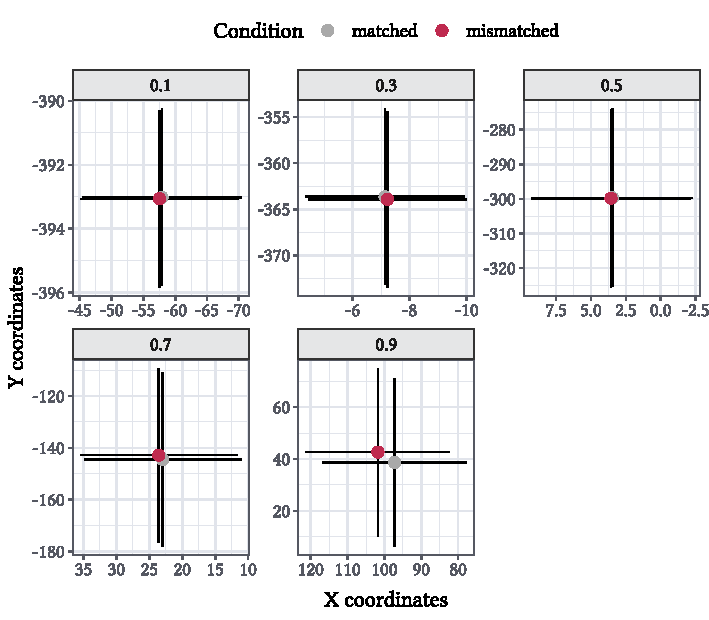
\includegraphics[]{figures/fig8.3.pdf}
    \caption{Effect of \textsc{condition} as found in the QGAMs modelled to the X and Y coordinates of \textsc{subset\textsubscript{IP}}. The lines indicate the confidence intervals of the estimated X and Y coordinate values.}
    \label{fig:8_3}
\end{figure}

\subsubsection{\textsc{subset\textsubscript{HP}}}\label{section08_2_2_2}

For \textsc{subset\textsubscript{HP}}, the found effects are given in Table \ref{tab:8.7}. The effect of \textsc{condition} reaches significance in three QGAMs fitted to X coordinates, i.e. in the $\tau=0.1,0.7$ and $0.9$ quantiles. For Y coordinates, significant effects are found in all QGAMs but the QGAM fitted to the $\tau=0.9$ quantile. The effects are illustrated in Figure \ref{fig:8_4}. For X coordinates in $\tau=0.1$, the effect of \textsc{condition} leads to coordinates further to the right. Taking into account more data, the effect is reversed in $\tau=0.7$ and $0.9$, i.e. coordinates of mismatched trials are further left. The effect of \textsc{condition} on Y values is similar across all quantiles. That is, mismatched trials show further up Y coordinates.

\begin{table}\fontsize{9}{10}
\caption{Summary of the effects found in the QGAMs fitted to the X and Y coordinates of \textsc{subset\textsubscript{HP}}. Significance codes: *** $p < 0.001$, ** $p < 0.01$, * $p < 0.05$.}
\label{tab:8.7}
\centering
\begin{tabular}{lrrrrrrrrrrr}
\lsptoprule
~                   & \multicolumn{5}{c}{X coordinates}       & \multicolumn{1}{c}{}                       & \multicolumn{5}{c}{Y coordinates}                               \\
\midrule
\multicolumn{1}{r}{quantiles:}          & 0.1        & 0.3        & 0.5        & 0.7        & 0.9 & ~       & 0.1        & 0.3        & 0.5        & 0.7        & 0.9         \\
\midrule
Parametric Terms    & \textbf{~} & \textbf{~} & \textbf{~} & \textbf{~} & \textbf{~} & \textbf{~} & \textbf{~} & \textbf{~} & \textbf{~} & \textbf{~}  \\
\midrule
(Intercept)         & ***        & ***        & ***        & ***        & *** & ~       & ***        & ***        & ***        & ***        & **          \\
\textsc{condition}\texttt{mismatched} & ***       & n.s.          & n.s.        & **        & ***  & ~      & *       & ***        & ***        & ***        & n.s.         \\
\midrule
Smooth Terms        & \textbf{~} & \textbf{~} & \textbf{~} & \textbf{~} & \textbf{~} & \textbf{~} & \textbf{~} & \textbf{~} & \textbf{~} & \textbf{~}  \\
\midrule
\textsc{order}               & ***        & ***        & ***        & ***        & ***   & ~     & ***        & ***        & ***        & ***        & ***         \\
\midrule
Random Smooth Terms & \textbf{~} & \textbf{~} & \textbf{~} & \textbf{~} & \textbf{~} & \textbf{~} & \textbf{~} & \textbf{~} & \textbf{~} & \textbf{~}  \\
\midrule
\textsc{item}                & ***        & ***        & ***        & ***        & ***  & ~      & ***        & ***        & ***        & ***        & ***         \\
\textsc{subject}             & ***        & ***        & ***        & ***        & ***  & ~      & ***        & ***        & ***        & ***        & ***        \\
\lspbottomrule
\end{tabular}
\end{table}

\begin{figure}
    \centering
    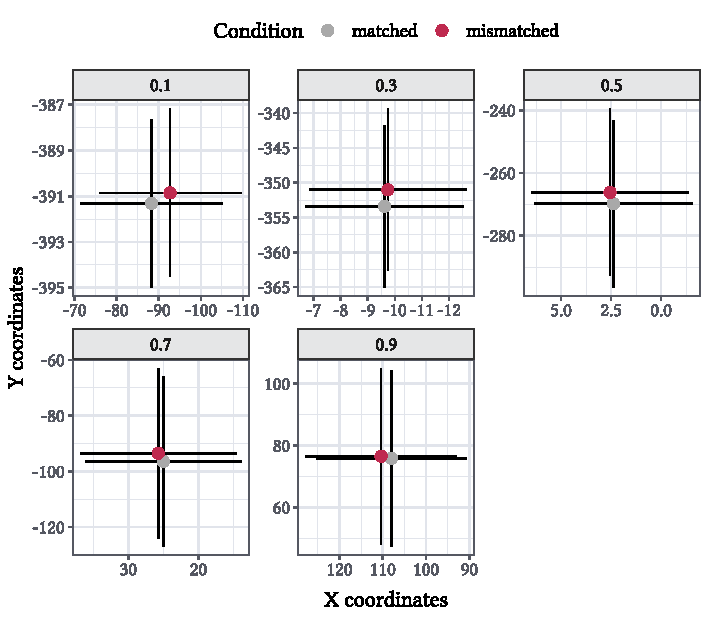
\includegraphics[]{figures/fig8.4.pdf}
    \caption{Effect of \textsc{condition} as found in the QGAMs modelled to the X and Y coordinates of \textsc{subset\textsubscript{HP}}. The lines indicate the confidence intervals of the estimated X and Y coordinate values.}
    \label{fig:8_4}
\end{figure}

\subsubsection{\textsc{subset\textsubscript{PI}}}\label{section08_2_2_3}

Table \ref{tab:8.8} presents the effects found for QGAMs fitted to the \textsc{subset\textsubscript{PI}} data. A significant effect of \textsc{condition} is found in quantiles $\tau=0.1,0.3$ and $0.5$ for X coordinates, and in all quantiles but $\tau=0.1$ for Y coordinates. The effects are displayed in Figure \ref{fig:8_5}. Where the effect of \textsc{condition} is significant for X values, coordinates of mismatched trials are further right. For Y coordinates, the effect of \textsc{condition} comes with coordinates further down for mismatched trial coordinates.

\begin{table}\fontsize{9}{10}
\caption{Summary of the effects found in the QGAMs fitted to the X and Y coordinates of \textsc{subset\textsubscript{PI}}. Significance codes: *** $p < 0.001$, ** $p < 0.01$, * $p < 0.05$.}
\label{tab:8.8}
\centering
\begin{tabular}{lrrrrrrrrrrr}
\lsptoprule
~                   & \multicolumn{5}{c}{X coordinates}    & \multicolumn{1}{c}{}                          & \multicolumn{5}{c}{Y coordinates}                               \\
\midrule
\multicolumn{1}{r}{quantiles:}          & 0.1        & 0.3        & 0.5        & 0.7        & 0.9  & ~      & 0.1        & 0.3        & 0.5        & 0.7        & 0.9         \\
\midrule
Parametric Terms    & \textbf{~} & \textbf{~} & \textbf{~} & \textbf{~} & \textbf{~} & \textbf{~} & \textbf{~} & \textbf{~} & \textbf{~} & \textbf{~}  \\
\midrule
(Intercept)         & ***        & n.s.         & ***        & ***        & ***    & ~    & ***        & ***        & ***        & ***        & n.s.          \\
\textsc{condition}\texttt{mismatched} & n.s.       & n.s.          & n.s.        & ***        & *** & ~       & ***       & ***        & ***        & ***        & n.s.         \\
\midrule
Smooth Terms        & \textbf{~} & \textbf{~} & \textbf{~} & \textbf{~} & \textbf{~} & \textbf{~} & \textbf{~} & \textbf{~} & \textbf{~} & \textbf{~}  \\
\midrule
\textsc{order}               & ***        & ***        & ***        & ***        & ***  & ~      & ***        & ***        & ***        & ***        & ***         \\
\midrule
Random Smooth Terms & \textbf{~} & \textbf{~} & \textbf{~} & \textbf{~} & \textbf{~} & \textbf{~} & \textbf{~} & \textbf{~} & \textbf{~} & \textbf{~}  \\
\midrule
\textsc{item}                & ***        & ***        & ***        & ***        & ***  & ~      & ***        & ***        & ***        & ***        & ***         \\
\textsc{subject}             & ***        & ***        & ***        & ***        & ***  & ~      & ***        & ***        & ***        & ***        & ***        \\
\lspbottomrule
\end{tabular}
\end{table}

\begin{figure}
    \centering
    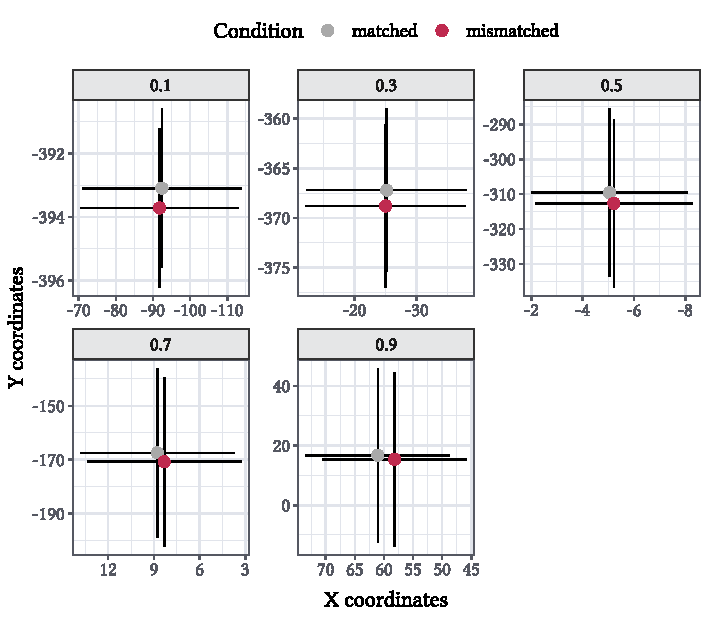
\includegraphics[]{figures/fig8.5.pdf}
    \caption{Effect of \textsc{condition} as found in the QGAMs modelled to the X and Y coordinates of \textsc{subset\textsubscript{PI}}. The lines indicate the confidence intervals of the estimated X and Y coordinate values.}
    \label{fig:8_5}
\end{figure}

\subsubsection{\textsc{subset\textsubscript{PH}}}\label{section08_2_2_4}

Finally, the effects found in the QGAMs fitted to the X and Y coordinates of the \textsc{subset\textsubscript{PH}} data are given in Table \ref{tab:8.9}. \textsc{condition} shows a significant effect on X coordinates in quantiles $\tau=0.5,0.7$ and $0.9$. For Y coordinates, a significant effect is found in all quantiles but $\tau=0.9$. The effects are illustrated in Figure \ref{fig:8_5}. For X coordinates, the effect of \textsc{condition} comes with coordinates further left for mismatched trials. For Y coordinates, the effect of \textsc{condition} leads to coordinates lower down for mismatched trials.

\begin{table}\fontsize{9}{10}
\caption{Summary of the effects found in the QGAMs fitted to the X and Y coordinates of \textsc{subset\textsubscript{PH}}. Significance codes: *** $p < 0.001$, ** $p < 0.01$, * $p < 0.05$.}
\label{tab:8.9}
\centering
\begin{tabular}{lrrrrrrrrrrr}
\lsptoprule
~                   & \multicolumn{5}{c}{X coordinates}       & \multicolumn{1}{c}{}                       & \multicolumn{5}{c}{Y coordinates}                               \\
\midrule
\multicolumn{1}{r}{quantiles:}          & 0.1        & 0.3        & 0.5        & 0.7        & 0.9  & ~       & 0.1        & 0.3        & 0.5        & 0.7        & 0.9         \\
\midrule
Parametric Terms    & \textbf{~} & \textbf{~} & \textbf{~} & \textbf{~} & \textbf{~} & \textbf{~} & \textbf{~} & \textbf{~} & \textbf{~} & \textbf{~}  \\
\midrule
(Intercept)         & ***        & n.s.         & ***        & ***        & *** & ~       & ***        & ***        & ***        & ***        & n.s.          \\
\textsc{condition}\texttt{mismatched} & **       & ***          & ***        & n.s.        & n.s.    & ~    & n.s.       & *        & ***        & ***        & ***         \\
\midrule
Smooth Terms        & \textbf{~} & \textbf{~} & \textbf{~} & \textbf{~} & \textbf{~} & \textbf{~} & \textbf{~} & \textbf{~} & \textbf{~} & \textbf{~}  \\
\midrule
\textsc{order}               & ***        & ***        & ***        & ***        & ***   & ~     & ***        & ***        & ***        & ***        & ***         \\
\midrule
Random Smooth Terms & \textbf{~} & \textbf{~} & \textbf{~} & \textbf{~} & \textbf{~} & \textbf{~} & \textbf{~} & \textbf{~} & \textbf{~} & \textbf{~}  \\
\midrule
\textsc{item}                & ***        & ***        & ***        & ***        & ***   & ~     & ***        & ***        & ***        & ***        & ***         \\
\textsc{subject}             & ***        & ***        & ***        & ***        & ***  & ~      & ***        & ***        & ***        & ***        & ***        \\
\lspbottomrule
\end{tabular}
\end{table}

\begin{figure}
    \centering
    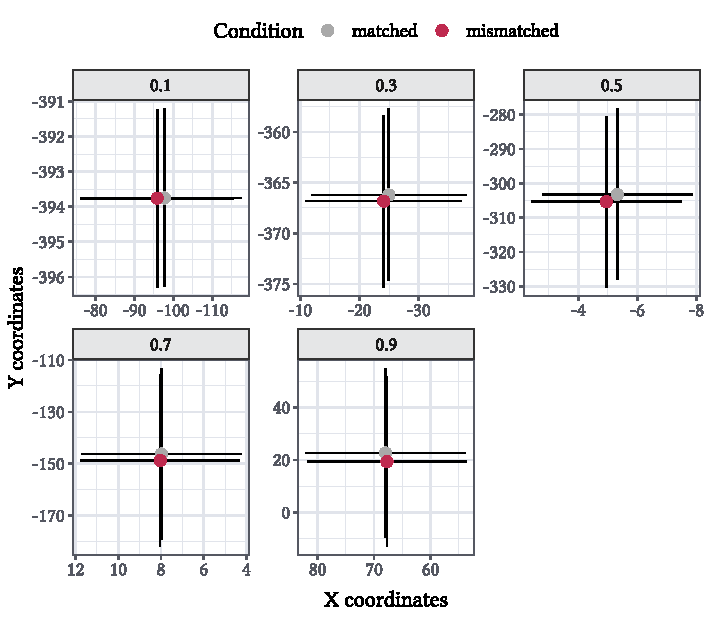
\includegraphics[]{figures/fig8.6.pdf}
    \caption{Effect of \textsc{condition} as found in the QGAMs modelled to the X and Y coordinates of \textsc{subset\textsubscript{PH}}. The lines indicate the confidence intervals of the estimated X and Y coordinate values.}
    \label{fig:8_6}
\end{figure}

\subsubsection{Overall results}\label{section08_2_2_5}

An overview of significant deviations found for the coordinates of mismatched stimuli trials across all quantiles and subsets is given in Table \ref{tab:8.10}. Considering the overall influence of \textsc{condition}, one can make two general observations. First, Y coordinates of mismatched stimuli trials are higher and, with the exception of $\tau=0.1$ for \textsc{subset\textsubscript{HP}}, further to the left if a mismatch is caused by a plural /s/ duration, as is the case in \textsc{subset\textsubscript{IP}} and \textsc{subset\textsubscript{HP}}. Second, Y coordinates of mismatched stimuli trials are lower if a mismatch is caused by an \textit{is}- or \textit{has}-clitic /s/ duration, as is the case in \textsc{subset\textsubscript{PI}} and \textsc{subset\textsubscript{PH}}, while for X coordinates no clear pattern is visible.

\begin{table}\fontsize{10}{11}
\caption{Overview of the direction of significant deviations found for coordinates in mismatched stimuli trials across all quantiles and subsets. Where no direction is given, no significant effect of \textsc{condition} was found.}
\label{tab:8.10}
\centering
\begin{tabular}{ccccccccc}
\lsptoprule
\multirow{2}{*}{~} & 
\multicolumn{2}{c}{\textsc{subset\textsubscript{IP}}} & 
\multicolumn{2}{c}{\textsc{subset\textsubscript{HP}}} & 
\multicolumn{2}{c}{\textsc{subset\textsubscript{PI}}} & 
\multicolumn{2}{c}{\textsc{subset\textsubscript{PH}}}  \\
\midrule
                                   $\tau$    & X    & Y                     & X     & Y                    & X     & Y                    & X    & Y                      \\
                                       \midrule
0.1                                    & ~    & ~                     & right & higher               & ~     & lower                & left & ~                      \\
0.3                                    & ~    & ~                     & ~     & higher               & ~     & lower                & left & lower                  \\
0.5                                    & ~    & ~                     & ~     & higher               & ~     & lower                & left & lower                  \\
0.7                                    & left & higher                & left  & higher               & right & lower                & ~    & lower                  \\
0.9                                    & left & higher                & left  & ~                    & right & ~                    & ~    & lower     \\
\lspbottomrule
\end{tabular}
\end{table}

\section{Discussion}\label{section08_3}

The number-decision task presented in this chapter investigated whether listeners make use of subphonemic durational differences in comprehension. It is different to the comprehension study presented in Chapter \ref{chapter07} by several aspects. First, pseudowords instead of real words were used as items. Thus, the effects found in the present study cannot be confounded by effects of lexical storage, frequency, or relatedness which are commonly associated with real words and their representations in the mental lexicon (see Section \ref{section03_1_1}). Second, items were presented in carrier sentences and not in isolation. This was necessary to disambiguate between different types of /s/ in the long run, as the number-decision process for pseudowords cannot rely on lexical knowledge. Third, plural, \textit{is}-, and \textit{has}-clitic word-final /s/ were part of the items, while the previous comprehension study investigated non-morphemic and plural word-final /s/. By investigating different types of /s/ across studies, one obtains a more detailed picture of potential effects. Despite these differences, both comprehension studies shared the same hypothesis. Building on extant models of speech perception and comprehension, \textsc{H comp}, the \textit{Mismatch Hypothesis}, was explored: If subphonemic durational differences are made use of, then a mismatch of subphonemic detail and intended meaning leads to a) slowed down comprehension processes, and b) deviated mouse trajectories. Part a) of the hypothesis was not investigated in the present study, as null results were found in the comprehension study of Chapter \ref{chapter07}. Thus, one question remained: Did a mismatch of subphonemic durational information lead to deviated mouse trajectories?

This question was investigated using QGAMs fitted to the X and Y coordinate data of the mouse-tracks recorded in the number-decision task. QGAMs were fitted separately for four subsets of data: 1) \textsc{subset\textsubscript{IP}}, 2) \textsc{subset\textsubscript{HP}}, 3) \textsc{subset\textsubscript{PI}}, and 4) \textsc{subset\textsubscript{PH}}, where the first subscript letter indicates the context and the second subscript letter indicates the mismatched type of /s/ (I = \textit{is}-clitic; H = \textit{has}-clitic; P = plural). In each of the subsets, trials of items with matched and mismatched /s/ duration were compared, while the items’ bases as well as the sentence the items were embedded within were kept constant. The overall results of the QGAMs show an effect of matched versus mismatched durational information across all four subsets. Taking a closer look at the nature of the found effects, one finds effects going into different directions between subsets (see Table \ref{tab:8.10}). For X coordinates, coordinate values of mismatched stimuli trials are further to the left for \textsc{subset\textsubscript{IP}}, \textsc{subset\textsubscript{HP}}, and \textsc{subset\textsubscript{PH}}. For \textsc{subset\textsubscript{PI}}, however, X coordinate values of mismatched trials are further to the right. For Y coordinates, one finds a difference between both clitic contexts and both plural contexts: Y coordinates are higher up when a mismatch is caused by a plural /s/ duration, but they are further down when the mismatch is caused by a clitic /s/ duration. Similar effects were found for QGAMs fitted post-hoc to the data for which the onset of the word-final /s/ has been heard already (see Section \ref{section07_3} for a discussion and the supplementary material given in Chapter \ref{Supplementary Material} for model overviews).

What do these findings mean in regard to the notion of deviated mouse-tracks due to mismatched subphonemic durational information? Recall that the mouse-tracks were mirrored where applicable, that is all tracks move towards the upper left corner of the coordinate system. Thus, an ideal non-deviated trajectory would be a straight line between the mouse cursor starting position and one of the answer options. As this non-deviated straight line moves linearly towards the upper left corner, X coordinates which are further to the left or right and Y coordinates which are further up or down can be understood as deviation from that direct path. If mismatched subphonemic durational information was to cause deviation from that ideal path, one would expect X coordinates to be further to the right and Y coordinates to be lower down, as such a deviation would express the expected effect of a mismatch: As context and /s/ duration do not match up, comprehension is influenced, and the mouse-track is deviated towards the incorrect response for the pertinent trial. Taking a trial with a clitic context as an example, a mismatch is caused by the plural /s/ duration of the target word’s word-final /s/. If comprehension is influenced by this durational mismatch, one would predict mouse movement towards the plural response due to the word-final /s/ duration. Once the entire context is processed, a correct answer is given. Moving the mouse away from the incorrect towards the correct response then results in an overall more deviated mouse-track.

How do the present findings relate to this prediction of a deviated path? For X coordinates, a deviation to the right was found for $\tau=0.9$ of \textsc{subset\textsubscript{HP}} and across \textsc{subset\textsubscript{PI}}. In all other significant cases, mismatched trials showed X coordinates further to the left instead. For Y coordinates, the expected lower coordinate values were found for \textsc{subset\textsubscript{PI}} and \textsc{subset\textsubscript{PH}}, while \textsc{subset\textsubscript{IP}} and \textsc{subset\textsubscript{HP}} showed higher Y coordinate values instead. That is, only the results for \textsc{subset\textsubscript{PI}} fully meet the expected directions of deviations. \textsc{subset\textsubscript{PH}} meets the directions for Y coordinates, but not for X coordinates. The two subsets in which a mismatch is caused by a plural /s/ duration, \textsc{subset\textsubscript{IP}} and \textsc{subset\textsubscript{HP}}, show deviations of the opposite directions instead: X coordinates are mainly further to the left and Y coordinates are higher up. Nonetheless, the \textit{Mismatch Hypothesis} is confirmed by the overall findings: Comparing mouse-tracks of matched and mismatched stimuli trials, one finds that they significantly deviate from each other across more than half of all QGAMs. 

However, how can one explain the opposing findings between \textsc{subset\textsubscript{IP}} and \textsc{subset\textsubscript{HP}} on the one, and \textsc{subset\textsubscript{PI}} and \textsc{subset\textsubscript{HP}} on the other hand? Noticeably, the effects found within the two clitic context subsets, as well as the effects found within the two plural context subsets are mostly similar. General differences in effect directions for Y coordinates are only found between these two groups. One potential explanation that comes to mind is the overall frequency of plural and clitic /s/ in the language. In the British National Corpus (\cite{Davies2004}), \textit{is}-clitic <’s> is attested 311,146 times and \textit{has}-clitic <’s> is attested 22,816 times. For plural <s>, the most frequent entry alone, \textit{things}, has a frequency of 40,453 which is almost double the frequency of the \textit{has}-clitic. Considering just plural /s/, one finds a frequency of about 140,000 when taking into account the top ten most frequent /s/ plural forms alone. That is, plural /s/ is overall far more frequent than clitic /s/. If a pseudoword contains the duration of a plural /s/, mouse-tracks deviate differently than predicted, i.e. further to the left and further up, as plural /s/ duration is the expected duration. The plural /s/ duration is expected as it is more frequent across the language. If a pseudoword contains the duration of a clitic /s/, mouse-tracks are deviated as predicted, i.e. further down, as this is a less expected duration due to the relatively low frequency of the clitic /s/ duration. Note that this is but an idea which requires further investigation.

Overall, the present results confirm that comprehension is significantly influenced by a mismatch of subphonemic durational information in word-final /s/. This finding is in line with the results of the mouse-track analysis presented for the comprehension study in Chapter \ref{chapter07} of this book. The nature of the found deviations, however, remains unaccounted for and requires further research.

Let us now turn to the theoretical implications of the present findings. Abstractionist theories which exclude subphonemic durational information from the perception and comprehension process cannot account for the present findings (e.g. \cite{Klatt1979, McClelland1986, Norris1994, Norris2008}). If such durational differences are not perceived, they cannot be used in comprehension. As significant differences between mouse-tracks of trials with matched versus mismatched durational information were found, such abstractionist approaches cannot explain the present results.

Exemplar and hybrid models (e.g. \cite{Goldinger1996, Hawkins2001, Pierrehumbert2002, Hanique2013Aalders}) and computational models (DIANA, \cite{tenBosch2015, tenBosch2021}; LDL, \cite{Baayen2019}) could in principle account for the present results. These approaches assume the storage of subphonemic detail. Such detail can be perceived and made use of in comprehension. However, it remains unclear how exemplar and hybrid models would account for the reverse effects found for clitic versus plural contexts. Computational models, however, might be able to shed further light on this issue. Taking LDL as a starting point, one could use the phonological and semantic measures derived from an implementation such as the one given in Chapter \ref{chapter05} as predictors to model coordinate data. Considering that one of these measures apparently reflects the distinction between non-morphemic and plural /s/ (see Section \ref{section05_4}), it might very well be the case that another measure can capture the effect of durational matches and mismatches. However, for such an implementation additional steps are required. First, audio data instead of phonological triphones has to be used as input to provide information on subphonemic durational differences. Second, one has to find a way to include clitic /s/, because clitic /s/ has not been incorporated in LDL implementations yet. 

In sum, no theoretical account can straightforwardly explain the findings of the present number-decision task. Mouse-tracks are influenced by mismatched subphonemic durational information in pseudowords. However, the nature of this influence is unaccounted for: Opposing directions of effects are found when comparing mismatched trials of clitic contexts and plural contexts. An explanation for these reversed effects should be motivation for future research. Such research might benefit from new LDL implementations and derived measures. Overall, the present study showed that subphonemic durational information is used in comprehension, and that such results are found independently of effects of lexical storage, frequency, and relatedness. 

%\chapter{General discussion}\label{chapter09}

In this book, I set out to establish substantiated knowledge on subphonemic detail and its role in production, perception, and comprehension. To achieve this goal, I used real words and pseudowords as items where applicable and I conducted thorough statistical analyses using novel statistical techniques where appropriate. To investigate the production, perception, and comprehension of subphonemic detail I made use of word-final /s/ in English as it is not only found as non-morphemic segment, but also has numerous morphological functions: plural, genitive, genitive plural, third-person singular, as well as the clitics of \textit{is}, \textit{has}, and \textit{us} (as in \textit{let’s}). Using a subset of these different types of /s/ – non-morphemic, plural, \textit{is}-, and \textit{has}-clitic /s/ – I conducted five studies. The aims of these studies were to determine whether such different types of /s/ show differences in their acoustic duration in production (Chapter \ref{chapter04}), to gain further insight into how such durational differences come to be (Chapter \ref{chapter05}), to learn whether durational differences in word-final /s/ are perceptible (Chapter \ref{chapter06}), and to examine if durational differences in word-final /s/ are made use of in comprehension (Chapters \ref{chapter07} and \ref{chapter08}). All investigations were of an explorative nature, addressing hypotheses derived from relevant theories to provide elaborate discussions of the pertinent findings. In the following, the respective hypotheses are repeated and then discussed based on the findings of the individual studies. Finally, all results are brought together to draw an overall picture of the production, perception, and comprehension of subphonemic detail in word-final /s/.

The production study presented in Chapter \ref{chapter04} of this book investigated whether there are durational differences in the acoustics of non-morphemic, plural, \textit{is}-, and \textit{has}-clitic word-final /s/. Using pseudowords as items in a highly controlled production task, it was made sure that effects of lexical frequency, predictability, and storage did not confound the results. It was shown that non-morphemic /s/ was longest, plural /s/ was shorter, and clitic /s/ was shortest. While these differences were found to be significant, the difference between the \textit{is}- and the \textit{has}-clitic was not. The following hypotheses were investigated:

\begin{description}
\item\textsc{H prod\textsubscript{1}}: \textit{Feed-Forward Hypothesis} \newline
There is no durational difference between word-final non-morphemic /s/, plural /s/, and auxiliary clitic /s/.

\item\textsc{H prod\textsubscript{2}}: \textit{Prosodic Hypothesis} \newline
There are durational differences between different types of word-final /s/: 
non-morphemic /s/ is shorter than plural /s/, plural /s/ is shorter than auxiliary clitic /s/.

\item\textsc{H prod\textsubscript{3}}: \textit{Emergence Hypothesis} \newline
There are durational differences between different types of word-final /s/ (non-morphemic, plural, and auxiliary clitic).
\end{description}

\textsc{H prod\textsubscript{1}}, the \textit{Feed-Forward Hypothesis}, is rejected as it predicted no durational differences between different types of word-final /s/. If standard feed-forward models of speech production underlying this hypothesis were refined in such a way that post-lexical processes can arise from certain kinds of lexical information, only then the present findings could be accounted for. \textsc{H prod\textsubscript{2}}, the \textit{Prosodic Hypothesis}, is rejected as it predicted the opposite direction for durational differences, with non-morphemic /s/ being shortest and clitic /s/ being longest in duration. This pattern is clearly not compatible with the present results. The theories underlying \textsc{H prod\textsubscript{3}}, the \textit{Emergence Hypothesis}, can potentially account for the present findings. The fact that durational differences were found indicates that such differences might emerge through the mechanisms introduced by the theories underlying this hypothesis. However, claiming that the hypothesis is therefore confirmed would be a fallacy: Only an implementation of one of such underlying theories can show whether the particular theory and its mechanisms can account for the durational differences found in the present production study.

Hence, an implementation of one of the underlying theories, linear discriminative learning, was used to further investigate the hypothesis. This LDL implementation and its analysis were presented in Chapter \ref{chapter05} of this book. Using the non-morphemic and plural /s/ durational data elicited in the production study, the analyses of the LDL implementation resulted in three main findings. First, measures derived from an LDL network trained on real words and pseudowords are predictive of word-final /s/ duration in pseudowords. Such measures are indeed just as predictive of /s/ durations as are more traditional variables. Second, even though such LDL measures show about the same level of predictivity, the effect of the type of /s/ as a variable is not fully captured by them. That is, the type of the word-final /s/ remained a significant predictor when introduced among measures derived from the LDL network. This indicates that there is more to the type of /s/ than the variables used in the present implementation. Third, even though the type of /s/ is not fully captured by the LDL measures, especially one of these measures, the correlation with the semantic nearest neighbour, showed a high correlation with the type of /s/. Hence, intricate semantic properties of the types of /s/ under investigation are indeed captured by measures derived from the LDL network. Coming back to the hypothesis at hand, \textsc{H prod\textsubscript{3}}, the \textit{Emergence Hypothesis}, it is found that it can be confirmed in regard to one of its underlying theories, linear discriminative learning.

Taking the results on the production of word-final /s/ as a starting point, the perception study presented in Chapter \ref{chapter06} asked whether such durational differences are perceptible. For this, a same-different task with real words and pseudowords as items was conducted. For each item, a version with the pertinent prototypical duration of non-morphemic or plural /s/ was created. Then, four further versions were constructed with their word-final /s/ either being incrementally shortened (mono-morphemic items) or lengthened (plural items) by 10 ms, 20 ms, 35 ms, and 75 ms. The results indicate that, on average, listener sensitivity is rather low for durational differences of 10 ms and 20 ms, and slightly but significantly higher for a durational difference of 35 ms. For the 75 ms durational difference, a significantly improved sensitivity was found. The following hypotheses were investigated:

\begin{description}
\item\textsc{H perc\textsubscript{1}}: \textit{Abstractionist Hypothesis} \newline
Listeners are not sensitive to subphonemic durational differences between different types of word-final /s/.

\item\textsc{H perc\textsubscript{2}}: \textit{Phonetic Detail Hypothesis} \newline
Listeners are sensitive to subphonemic durational differences between different types of word-final /s/.
\end{description}

\textsc{H perc\textsubscript{1}}, the \textit{Abstractionist Hypothesis}, is rejected. The hypothesis was built on theories which assume that subphonemic durational differences are not perceptible. Due to the strictly phonological nature of perception found in such theories, these and the present findings are fully incompatible. \textsc{H perc\textsubscript{2}}, the \textit{Phonetic Detail Hypothesis}, can be confirmed under two premises. First, only an implementation of the models underlying the hypothesis can sufficiently confirm whether a particular model’s mechanisms can account for the present findings. Second, listeners showed sensitivity to subphonemic durational differences. However, major increases in sensitivity and overall high levels of sensitivity were only found for the biggest durational difference of 75 ms – a difference that is not found in studies on the durational differences between different types of /s/. Thus, according to the present findings, not all durational differences between different types of /s/ found in studies on their acoustic duration are assumed to be well perceptible. 

Importantly, there most likely is an issue of methodology at hand here. Same-different tasks such as the one used in the present perception study are metalinguistic tasks. Hence, certain properties of language are the main focus for parti-cipants of such tasks instead of language or language use itself. Thus, participants encountered a task they are not familiar with and that extends beyond their day-to-day usage of language: differentiating isolated words by the duration of their word-final /s/. It might thus very well be the case that a same-different task is not the most appropriate experimental setup to investigate the perceptibility of subphonemic durational differences.

A type of task that focuses more narrowly on language use itself was used in the two comprehension tasks presented in Chapters \ref{chapter07} and \ref{chapter08}. In number-decision tasks, participants were asked to decide whether an isolated word (Chapter \ref{chapter07}) or the agent in a sentence (Chapter \ref{chapter08}) was singular or plural. In the case of isolated words, words with non-morphemic and plural /s/ were used as target items. In the case of agents in a sentence, pseudowords with plural, \textit{is}-, and \textit{has}-clitic /s/ were used as target items. In both experiments, /s/ durations were either matched with their context, e.g. a plural word had an /s/ with a typical plural /s/ duration, or /s/ durations were mismatched with their context, e.g. a plural word had an /s/ with a typical non-morphemic or clitic /s/ duration. It was found that reaction time was not influenced by the durational mismatch of word-final /s/ and (pseudo-)base. Mouse-tracks, however, showed a significant effect of mismatched durations in that they followed significantly different paths as compared to the mouse-tracks of matched items. In both comprehension studies, the following hypothesis was investigated:

\begin{description}

\item\textsc{H comp}: \textit{Mismatch Hypothesis} \newline
If listeners make use of subphonemic durational differences in the comprehension of different types of word-final /s/, then a mismatch of subphonemic detail and intended meaning leads to\newline
a) slowed down comprehension processes.\newline
b) deviated mouse trajectories.

\end{description}

As no differences in reaction times were found in Chapter \ref{chapter07}, part a) of \textsc{H comp} cannot be confirmed. That is, the overall time to react to an audio stimulus with a mismatched /s/ duration is just as long as the time to react to an audio stimulus with a matched /s/ duration. Part b) of \textsc{H comp}, however, is confirmed by the findings, as mouse-tracks of both conditions, matched and mismatched, significantly differed, i.e. the mouse-tracks of the mismatched stimuli trials deviated from the mouse-tracks of the matched stimuli trials. While the patterning of deviation as such is not straightforwardly explainable, especially taking into account the results of Chapter \ref{chapter08}, an influence of mismatched subphonemic durational differences was found, nonetheless.

How do the findings of the individual studies relate to the overarching goal of this book to draw a more detailed, intricate, and exhaustive picture of the production, perception, and comprehension of subphonemic detail? For production, it was found that different types of word-final /s/ are indeed different in terms of their acoustic duration. The nature of these differences is in line with previous corpus studies, but not with previous experimental studies. Analysing the durational differences not only by means of traditional variables but also by using measures derived from an LDL implementation, it was shown that such measures are predictive of word-final /s/ durations. Thus, the origin of durational differences in word-final /s/ can most likely be explained by the resonance of words with the lexicon. Taking into account the highly controlled methodology of the production study, its results, the measures derived from the LDL implementation, and the analyses of these measures, the first general aim of this book can be addressed: Subphonemic durational differences between different types of word-final /s/ exist. A potential explanation for the contradictory nature of previous results lies within the applied methodology and statistical analyses used in previous experimental studies. While these previous studies used homophonous real words as target items, I used pseudowords instead, avoiding the potential issues and uncertainties regarding the representation of homophones within the mental lexicon. Making use of an LDL implementation, pseudowords were shown not to be semantically empty, but to resonate with the lexicon. The measures derived from the LDL implementation, then, allowed for further insight into the origin of such durational differences. That is, higher degrees of semantic activation diversity and higher levels of phonological certainty come with shorter /s/ durations.

For perception, it was found that listeners showed higher sensitivity for durational differences of 35 ms and 75 ms as compared to the smaller differences of 10 ms and 20 ms. The results indicate that durational differences of 35 ms are somewhat perceptible, while durational differences of 75 ms show a further increased level of perceptibility. These results are more or less in line with the findings by \citet{Klatt1975} in that these authors claimed 25 ms to be the just-noticeable durational difference to a segment. As \citet{Klatt1975} also noted that durational differences in word-final fricatives are less well perceptible, the increase in sensitivity and thus perceptibility found for 35 ms is close to their 25 ms, but the threshold is most likely higher due to /s/ being word-final and a fricative. Regarding the second general aim of this book, then, one can conclude that the durational difference to a single segment to be perceptible should be at least of 35 ms if it is a fricative in word-final position. Note, however, the aforementioned issue of the metalinguistic nature of the same-different task on why the overall sensitivity was found to be rather low.

For comprehension, it was found that subphonemic durational differences indeed influence comprehension. Using target items with matched and mismatched durational /s/ information, it was found that mouse-trajectories for matched versus mismatched items were significantly different across all types of /s/ under investigation. This finding suggests that durational differences are used in comprehension, and should thus also be perceptible even though the overall low sensitivity values obtained in the perception task might suggest otherwise. Reaction times, on the other hand, did not significantly differ between matched versus mismatched item trials. However, reaction times only represent a single data point per trial while mouse-tracks give insight into the decision-making process during comprehension. Regarding the third general aim of this book, then, one may conclude that comprehension is influenced by subphonemic durational differences. More precisely, while the time between perception and the outcome of comprehension is not significantly influenced, the comprehension process between the input of an audio stimulus and the outcome of comprehension appears to be significantly affected.

So what does the overall picture of the production, perception, and comprehension of subphonemic detail look like? Subphonemic detail is influenced by morphological make-up as different types of word-final /s/ show differences in their acoustic durations and is perceptible if durational differences are above a certain threshold. Subphonemic detail influences and is made use of in the process of comprehension. As was demonstrated, these overall results ultimately call for revisions of models of speech production, perception, and comprehension which do not incorporate subphonemic detail in their pertinent representations and processes.  

%\chapter{Conclusion}\label{chapter10}

This book set out to investigate the production, perception, and comprehension of subphonemic detail. To operationalise the investigation, word-final /s/ in English was used in real word and pseudoword target items for a production task, an implementation of linear discriminative learning, a same-different task, and two number-decision tasks.

The first general aim of the present book was to examine whether durational differences in morphologically different types of word-final /s/ – non-morphemic, plural, \textit{is}-, and \textit{has}-clitic /s/ – can be found and how such differences can be accounted for. While previous studies reported such differences, the nature of these differences deviated between previous corpus studies and previous experimental studies. The results obtained in the production task presented in this book are in line with the findings of previous corpus studies. That is, non-morphemic /s/ is longest in duration, clitic /s/ is shortest in duration, and plural /s/ duration is in between non-morphemic /s/ and clitic /s/ durations. The two clitics under investigation were found not to be significantly different in terms of their durations. Turning to the results of the LDL implementation, it seems that the durational differences are connected to a word’s resonance with the lexicon in that its semantic activation diversity and its phonological certainty are predictors of its word-final /s/ duration.

The second general aim of this book was to investigate how small a durational difference in word-final /s/ is perceptible. Using a same-different task, it was found that listeners showed a higher sensitivity for a durational difference of 35 ms as compared to smaller durational differences. This finding is more or less in line with previous work in that the just-noticeable durational difference should be at about 25 ms, but higher for word-final fricatives as is the case for word-final /s/.

The third general aim of this book was to find out whether subphonemic durational differences significantly influence comprehension. To investigate this issue, two number-decision tasks in a mouse-tracking paradigm were used. One task made use of isolated real words with either durationally matched or mismatched non-morphemic and plural /s/ duration, while the other task used pseudowords embedded within sentences with either durationally matched or mismatched plural, \textit{is}-, and \textit{has}-clitic /s/ duration as target items. It was found that reaction times are not influenced by the mismatch of durational information. However, both comprehension studies found a significant difference between mouse-tracks of trials of matched versus trials of mismatched durational information. Thus, the process of comprehension itself apparently is influenced by subphonemic detail, while the duration of the process of comprehension is not.

The investigation of the general aims revealed that a discernible number of extant models of speech production, perception, and comprehension cannot account for the present findings. Subphonemic durational differences are not predicted at all, or their directions are either unpredicted or said to be the opposite of what was found. The perception of subphonemic durational detail is ruled out completely, and an influence on comprehension is thus not considered. In light of the findings presented in this book, then, such models need to be revised. Yet, some promising, especially computational, approaches already exist. Future implementations of such accounts will show whether and how such approaches can be used to explain the intricacy of language structure.
The complexities of speech production, perception, and comprehension remain enormous. The present book may have shed light on only a few of many issues: the production, perception, and comprehension of subphonemic detail. It was demonstrated by the findings of this book that various theoretical approaches to the production, perception, and comprehension of language and its fine-grained phonetic detail are in need of revision. 

%\chapter{Supplementary material}\label{Supplementary Material}

The supplementary material for this book consists of additional tables sorted by chapters, scripts and data for all analyses, and a markdown documentation of the LDL implementation - all originally created for the dissertation this book is based on. 

The supplementary material is available at: \url{https://osf.io/rc7xj/}


%\include{chapters/test}
%\include{chapters/tabless}

%%%%%%%%%%%%%%%%%%%%%%%%%%%%%%%%%%%%%%%%%%%%%%%%%%%
%%             Backmatter                       %%%
%%%%%%%%%%%%%%%%%%%%%%%%%%%%%%%%%%%%%%%%%%%%%%%%%%%

% \input{localseealso.tex}
% % There is normally no need to change the backmatter section
\input{backmatter.tex}
\end{document} 
